\documentclass[11pt]{article}
\usepackage[utf8]{inputenc}
\usepackage[T1]{fontenc}
\usepackage{geometry}
\usepackage{amsmath}
\usepackage[version=4]{mhchem}
\usepackage{amsfonts}
\usepackage{amssymb}
\usepackage{graphicx}
\usepackage{xcolor}
% \usepackage{natbib}
\usepackage{url}
\usepackage{hyperref}
\usepackage{titlesec}
\usepackage{enumitem}
\usepackage{wrapfig}
\usepackage[backend=biber, style=numeric, sorting=none]{biblatex}
\addbibresource{ref.bib}

\usepackage{booktabs}
\usepackage{array}
\usepackage{caption}
\usepackage{subcaption}
\usepackage{lmodern}
\usepackage{microtype}
\usepackage{threeparttable}   % for threeparttable and tablenotes
\captionsetup{font=scriptsize, labelfont=bf, position=top, skip=3pt}
\setlength{\tabcolsep}{4pt}
\renewcommand{\arraystretch}{1.05}

% Page layout
\geometry{
    left=0.8in,
    right=0.6in,
    top=0.6in,
    bottom=0.8in
}
\newcommand{\ts}{\mathrm{TS}}
\newcommand{\jsd}{\mathrm{JSD}}
\newcommand{\tsw}{\mathrm{TS_{wild}}}
\newcommand{\inm}{\mathrm{Infl}}
\newcommand{\adj}{\mathrm{Adj}}
\newcommand{\K}[1]{{\color{red}[[\textbf{K: }#1]]}}
\newcommand{\E}[1]{{\color{blue}#1}}
\newcommand{\facin}{f(\mathrm{act/inh})}
\newcommand{\ewnum}{\mathrm{EW_{num}}}
\newcommand{\tsten}{\mathrm{Toggle Switch (10N,100E)}}
\newcommand{\tstwo}{\mathrm{Toggle Switch (10N,80E)}}
\newcommand{\tsfour}{\mathrm{Toggle Switch (10N,60E)}}
\newcommand{\tssix}{\mathrm{Toggle Switch (10N,40E)}}
\newcommand{\tseight}{\mathrm{Toggle Switch (10N,20E)}}
\newcommand{\emttwosix}{\mathrm{EMT (23N,89E)}}
\newcommand{\emtrac}{\mathrm{EMT (17N,62E)}}
\newcommand{\gonad}{\mathrm{Gonadal (18N,74E)}}
\newcommand{\siltwo}{\mathrm{Silviera (18N,37E)}}
\newcommand{\sil}{\mathrm{Silviera (16N,30E)}}
\newcommand{\sclc}{\mathrm{SCLC (33N,357E)}}
\newcommand{\tennode}{\mathrm{NRF2 + OVOL (8N,19E)}}
\newcommand{\twenode}{\mathrm{NRF2 + GRHL2 + OVOL (11N,28E)}}
\newcommand{\beginsupplement}{%
        \setcounter{table}{0}
        \renewcommand{\thetable}{S\arabic{table}}%
        \setcounter{figure}{0}
        \renewcommand{\thefigure}{S\arabic{figure}}%
        \setcounter{section}{0}
        \renewcommand{\thesection}{S\arabic{section}}%
     }

%%%%%%%%%%%%%%%%%%%%%%%%%%%%%%%%%%%%%%%%%%%%%%%%%%
\title{Regulatory stochasticity drives opposing phenotypic outcomes in cell-fate decision networks}

\author{Kishore Hari$^1$, Abhay Gupta$^2$, Lakshmi Malvadi Shivakumar$^3$, Prakash Kulkarni$^{4~\&~5}$, Ravi Salgia$^4$, \\ Mohit Kumar Jolly$^3$, Herbert Levine$^1$}



\begin{document}


\maketitle
\begin{center}
    $^1$ Center for Theoretical Biological Physics \& Department of Physics, Northeastern University, Boston, MA, USA\\
    $^2$ Indian Institute of Science Education and Research Mohali, Mohali, PB, India\\
    $^3$ Department of Bioengineering, Indian Institute of Science, Bengaluru, KA, India \\
    $^4$ Department of Medical Oncology and Therapeutics Research, Hope National Medical Center, Duarte, CA, USA
    $^5$ Department of Systems Biology, City of Hope National Medical Center, Duarte, CA, USA 
\end{center}
\begin{center}
    \small \textbf{Current address:} Abhay Gupta - Department of Biology, University of Virginia, Charlottesville, USA\\
    \small \textbf{Current Address:} Lakshmi Malvadi - Department of Physics, University of California Merced, Merced, USA\\
\end{center}
\begin{abstract}
Models of gene regulatory networks (GRNs) underlying cell-fate decisions treat regulatory parameters as fixed quantities, although the effective strength of transcriptional regulation varies with molecular context. We asked how temporal fluctuations in interaction strength, rather than in molecular abundance, alter phenotype occupancy in multistable regulatory networks. We applied three stochastic update rules to the fold-change parameters of RACIPE ensembles of mutually inhibitory circuits---fluctuations anchored to their initial values, a bounded additive random walk, and a multiplicative walk that strengthens interactions toward a maximal strength---and tested analogous perturbations in Boolean models of epithelial--mesenchymal plasticity and gonadal-fate determination. Anchored fluctuations largely preserved deterministic occupancies of network states. Additive fluctuations increased occupancy of all-high co-expression states, an effect that extended to hybrid team-expression states in both biological networks. Multiplicative fluctuations favored single-high states in a topology-dependent manner, by an amount set by the maximal interaction strength. Control simulations with fixed, mean or periodically resampled fold-changes showed that both effects arise mainly from the shift in the distribution of regulatory strengths, and that the timescale of fluctuation relative to expression determines what is added on top. When fold-changes vary faster than expression relaxes, additive noise further enriches all-high states, because derepression acts independently of the regulator whereas repression requires it, while fast multiplicative noise weakens the single-high shift. Thus, both the distribution and the timescale of regulatory fluctuations shape phenotype occupancy, with outcomes constrained by network topology.
\end{abstract}

\section{Introduction}\label{sec:Intro}

GRNs are biological regulatory circuits that constitute a complex collection of molecular regulators including transcription factors (TFs), signaling molecules, and DNA segments that interact to regulate gene expression. They determine the spatiotemporal patterns of gene expression involved in determining cellular development, identity, and environmental responses. They also play a central role in determining the organism’s body plan, which is central to evolutionary developmental biology \cite{Davidson2005, Davidson2006, Maizels2026}. GRNs are conventionally modeled as deterministic systems with fixed interaction parameters although it is clear that the effective strength of any regulatory interaction is subject to continuous fluctuation in vivo. Nonetheless, an overwhelming fraction ($\approx$90\%) of TFs are intrinsically disordered proteins (IDPs) \cite{Staby2017} with significant disordered regions \cite{Ferrie2022Structure-functionRegulation, Holehouse2023TheRegions}. % REVISION (R2.1): IDPs, PTMs and chromatin presented as sources of variable regulatory strength that motivate the model, not as its subject.
These disordered regions mediate conformationally heterogeneous, post-translational modification (PTM)-sensitive contacts with DNA and co-factors. Interaction strength need not be tied to a single bound structure: two disordered proteins can bind with picomolar affinity while remaining fully disordered~\cite{Borgia2018Extreme}, and phosphorylation can fold a disordered region and switch its binding to a partner~\cite{Bah2015Folding}. The effective affinity of such regulators therefore depends on their conformational and modification state rather than taking a single fixed value. Although the individual conformers in an IDP ensemble are in fast exchange, certain conformations are stabilized by specific PTMs, especially phosphorylation, that exist with half-lives that range from minutes to hours, contributing to ``conformational noise'' \cite{Kulkarni2022, Kulkarni2019}. Non-specific TF binding to genomic decoy sites further modulates the effective regulatory signal in an affinity- and abundance-dependent manner \cite{Dey2020EnhancementSites, Burger2012InfluenceExpression}. Enhancer dynamics and transcriptional bursting add a third layer, coupling stochastic TF occupancy at cis-regulatory elements directly to fluctuations in target gene activation \cite{Raj2006StochasticCells, Fukaya2016EnhancerBursting}. The availability of TF binding sites can also vary over the course of transcription, due to noise in chromatin folding states \cite{Gamble2025}. Collectively, these mechanisms suggest that the effective strengths of regulatory interactions vary in time. Consequently, the impact of such regulatory noise—temporal stochasticity in these parameters—on the dynamics of multistable GRN motifs underlying cell-fate decisions remains poorly understood.


This question is especially relevant in the context of cancer, where genetic instability, aberrant chromatin remodeling, and rewired signaling cascades collectively amplify both intrinsic gene expression noise and extrinsic cell-to-cell variability \cite{Brock2009Non-geneticTumours, Landau2014LocallyLeukemia, Hanahan2026HallmarksBeyond}. Non-genetic heterogeneity — stable phenotypic variation within a clonal population arising from gene expression noise and network multi-stability — is now recognized as a major contributor to drug tolerance and tumor progression \cite{Hanahan2026HallmarksBeyond, Franca2024CellularContinuum, Shaffer2017RareResistance}. In this setting, the parameters of regulatory interactions that govern the dynamics of non-genetic heterogeneity cannot be considered fixed: PTM landscapes, co-factor availability, and chromatin accessibility to TFs all fluctuate, effectively introducing stochasticity into the fold-change parameters that govern network behavior. 


Perhaps a natural starting point to studying how regulatory noise propagates through GRNs is the toggle switch — a simple mutually repressive circuit between two master regulators that is among the most commonly occurring and extensively characterized motifs for binary cell-fate decisions \cite{gardner2000construction}. The toggle switch exhibits bistability under a broad range of kinetic parameters, and noise-induced switching between its two attractors has been studied in detail in both synthetic and natural contexts \cite{tian2006stochastic}. Many biological decisions, however, are not binary. For example, T helper cell differentiation, haematopoietic lineage commitment, and epithelial–mesenchymal–hybrid state transitions all involve three or more stable phenotypes. The addition of self-activation to the toggle switch (TSSA, toggle switch with self-activation) stabilizes the intermediate phenotype --- corresponding to hybrid phenotypes in EMT and progenitor states in differentiation cascades --- where both nodes are co-expressed simultaneously~\cite{Lu2013}. Three nodes connected to each other via a toggle switch, forming the toggle triad (TT). TT enables three distinct cell states, each defined by one node being highly expressed and the other two repressed \cite{doi:10.1098/rsif.2020.0631}. Importantly although GRNs underlying cell-fate decision systems often involve a larger number of TFs than accounted for in these motifs, TFs corresponding to a phenotype often form teams such that nodes belonging to the same team activate each other. These teams mutually inhibit each other, thereby forming higher order forms of the motifs listed above. These higher order motifs have similar qualitative behavior as their small motif counterparts such as a two team network promoting bistability with a small fraction of intermediate states, similar to TSSA. 


The effect of stochasticity on toggle switch dynamics has been studied extensively, though almost exclusively through noise applied to molecular copy numbers rather than interaction parameters. Early work established that intrinsic noise — arising from the discreteness of protein and mRNA molecules — can drive spontaneous switching between the attractors of a multistable circuit, with switching rates that decrease exponentially with copy number and increase with noise magnitude \cite{tian2006stochastic, Wang2007Noise-inducedSwitch}. Analytical treatments using the Chemical Langevin Equation and mean first-passage time theory have characterized how the depth and asymmetry of the potential wells governing each attractor determine residence times and transition rates \cite{Wang2010TheDifferentiation, Strasser2012StabilityExpression, Xu2014SwitchSwitch}. A key finding across these studies is that noise type — not only noise magnitude — shapes attractor occupancy: additive and multiplicative noise applied to the same deterministic system produce different effective potential landscapes and therefore different stationary probability distributions \cite{Jaruszewicz2013ToggleGene}. Extending beyond Gaussian noise, Lévy noise models have shown that heavy-tailed fluctuations can induce coherent switching at substantially lower intensities than Gaussian noise requires, by enabling large jumps that entirely overcome the potential barrier~\cite{Xu2016TheNoise}. At the network level, toggle switch dynamics has been studied under coupled and multicellular settings, where intracellular multiplicative noise can induce synchronized switching across cell populations via quorum-sensing pathways \cite{Wang2007Noise-inducedSwitch}. More recently, the sRACIPE framework demonstrated that expression-level (state) noise merges bistable clusters at high intensity, while static parametric variation across the model ensemble instead broadens clusters without destabilizing them \cite{Kohar2018RoleCircuits}. In both cases, however, the kinetic parameters themselves remain fixed once sampled; neither treats the parameter as a time-evolving stochastic process, which is the gap that our regulatory noise framework addresses. Stochastic analysis of the toggle triad and related tristable motifs has received comparatively little attention, with existing studies focused primarily on deterministic bifurcation structure and attractor geometry \cite{doi:10.1098/rsif.2020.0631, Duddu2025DistinctNetworks} rather than noise-driven state transitions. Whether the richer transition topology of the toggle triad — permitting direct switching between all three attractor pairs — confers qualitatively different susceptibility to regulatory noise compared to the toggle switch remains an open question.


In this manuscript, we study how regulatory noise – that is, the fluctuations of the parameters governing the interactions in GRNs – systematically shapes the dynamics of these motifs. We focus on the fold-change parameter \cite{Huang2017}, which describes the change in the production rate of a target node due to an upstream transcription factor. We couple stochastic fold-change perturbations with the Random Circuit Perturbation (RACIPE) framework \cite{Huang2017}. RACIPE generates large ensembles of ODE models with randomly sampled kinetic parameters, enabling topology-level inferences that are robust to parameter uncertainty. By superimposing continuous stochastic noise on the fold-change parameters of these ensembles, we successfully isolated the effect of regulatory noise from parameter-set-specific idiosyncrasies and characterized how mean residence times and switching frequencies depend on noise magnitude, noise mode, and attractor stability class. Control simulations that hold the fold-changes fixed at values drawn from the noise-induced distribution, set them to their mean, or resample them at fixed intervals separate the contribution of the distribution of regulatory strengths from that of their variation in time. We find that the type of regulatory noise and its timescale relative to gene expression, and not only its magnitude, determine phenotype occupancy in cell-fate circuits.

\section{Methods}

\subsection{Network models and RACIPE ensemble generation}\label{sec:RACIPE}

Each network motif is modeled as a system of ordinary differential equations (ODE), one ODE per node, following the shifted Hill formalism of RACIPE~\cite{Huang2017}:
\begin{equation}
\frac{dX}{dt} = g_X \prod_{i \in P} \frac{H(Y_i, Y_{i0}, n_{Y_i}, \lambda_{Y_i})}{\lambda_{Y_i}} \prod_{i \in N} H(Y_i, Y_{i0}, n_{Y_i}, \lambda_{Y_i}) - d_X X
\label{eq:odeM}
\end{equation}
\begin{equation}
H(Y_i, Y_{i0}, n_{Y_i}, \lambda_{Y_i}) = \lambda_{Y_i} \frac{Y_i^{\,n_{Y_i}}}{Y_{i0}^{\,n_{Y_i}} + Y_i^{\,n_{Y_i}}} + \frac{Y_{i0}^{\,n_{Y_i}}}{Y_{i0}^{\,n_{Y_i}} + Y_i^{\,n_{Y_i}}}
\label{eq:hillM}
\end{equation}
where $g_X$ and $d_X$ are the production and degradation rates of node $X$, $P$ and $N$ index its activating and inhibiting regulators, and $\lambda_{Y_i}$ is the fold-change by which regulator $Y_i$ modulates $X$'s production ($\lambda_{Y_i} > 1$ for activation, $\lambda_{Y_i} < 1$ for inhibition).

For each network topology, RACIPE~\cite{Huang2017} was used to generate an ensemble of $10{,}000$ parameter sets by uniform sampling within standard biologically plausible ranges, with each parameter set solved from 100 random initial conditions to identify its steady-state attractor(s). The resultant ensemble of steady states was used to calculate thresholds of individual node expressions ($\theta_X$) as the average expression across the ensemble, which were then used to discretize the steady states into strings of 1's and 0's. Based on the number of such discretized steady states allowed, each parameter set was assigned a multistability class (monostable, bistable, tristable, tetrastable). A representative subset of up to 1000 parameter sets was selected from each stability class present for a given network for downstream stochastic analysis (fewer where a stability class had fewer available parameter sets).

\subsection{Regulatory noise model} \label{sec:noise}

To simulate regulatory noise, we allowed the fold-change parameters $\lambda_{Y_i}$ to vary stochastically over time rather than remaining fixed at their RACIPE-sampled value, using a periodic update applied every $dt = 0.01$ (a.u.) during ODE integration. Three noise modes were implemented, differing in how each update depends on the parameter's current value:
\begin{align}
\text{Stationary:} \quad & \lambda(t+dt) = \lambda(0) + \mathcal{N}(0, \sigma_{\text{eff}}^2),\\
\text{Multiplicative:} \quad & \mu(t+dt) = \mu(t)\left(1 + \mathcal{N}(0, \sigma^2)\right), \quad \mu = \lambda \text{ (inhibitory)},\ \mu = 1/\lambda \text{ (activatory)}\\
\text{Additive:} \quad & \lambda(t+dt) = \lambda(t) + \mathcal{N}(0, \sigma_{\text{eff}}^2)
\end{align}
where $\sigma_{\text{eff}} = \sigma \cdot \lambda_{\max}$, with $\lambda_{\max}$ the upper bound of the relevant fold-change (inhibitory: $\lambda_{\max} = 1$, so $\sigma_{\text{eff}} \approx \sigma$; activatory: $\lambda_{\max} = 100$), so that a given nominal noise level $\sigma$ corresponds to a comparable proportion of each parameter's admissible range regardless of whether it governs activation or inhibition.  This scaling applies to additive and stationary noise. For multiplicative noise, $\sigma$ is a relative step and is not rescaled: the quantity that full regulation drives to its limit, $\mu = \lambda$ for inhibitory and $\mu = 1/\lambda$ for activatory edges, is multiplied by $(1 + \sigma\eta)$ with $\eta \sim \mathcal{N}(0,1)$ at every update, so that $\lambda(t+dt) = \lambda(t)(1+\sigma\eta)$ for inhibition and $\lambda(t+dt) = \lambda(t)/(1+\sigma\eta)$ for activation. For $\sigma = 0$ all three rules reduce to $\lambda(t+dt) = \lambda(t)$. Away from the bounds the multiplicative rule is unbiased in the mean, $\mathbb{E}[\mu(t+dt)] = \mu(t)$, but $\log\mu$ drifts by approximately $-\sigma^2/2$ per update, so the typical value of $\mu$ decreases and edges accumulate near maximal regulatory strength. After each update, $\lambda$ was set to the nearest bound if it left the admissible range ($[0.01, 1]$ for inhibitory and $[1, 100]$ for activatory parameters under additive and stationary noise; $[10^{-3}, 1]$ and $[1, 10^{3}]$ under multiplicative noise, where a factor $1+\sigma\eta \le 0$ sets the edge to maximal strength). The bounds are not absorbing: later updates can move $\lambda$ back into the interior. Noise levels $\sigma \in \{0, 0.001, 0.005, 0.01, 0.05, 0.1, 0.5, 1\}$ were tested for each noise mode and network.

% REVISION (R1.3, R3.1): interpretation of the multiplicative bound.
Under multiplicative noise the bound $\mu_{\min} = 10^{-3}$ is not a range for $\lambda$ to fluctuate through but the limit it is driven to. Per update, $\log\mu$ has drift $-\sigma^2/2$ and variance $\sigma^2$, both proportional to $\sigma^2$. Treated as a drifted Brownian motion confined to $[\log\mu_{\min}, 0]$, it therefore has a stationary density that does not depend on $\sigma$, $p(\mu) \propto \mu^{-2}$ on $[\mu_{\min}, 1]$. Half of this density lies within twofold of $\mu_{\min}$ and 90\% within tenfold, and its mean, $\mu_{\min}\ln(1/\mu_{\min})/(1-\mu_{\min}) \approx 0.007$, corresponds to about 145-fold regulation. Direct simulation of the update rule reproduces this law for $\sigma \geq 0.05$ at $dt = 0.01$ (median $\mu$ 1.6--1.9 times $\mu_{\min}$). The $\lambda$ process depends on the noise amplitude and update interval only through $\sigma^2/dt$, which sets how fast the limit is approached: starting from $\mu_0$, the median reaches it after about $2\ln(\mu_0/\mu_{\min})\,dt/\sigma^2$ time units, roughly 900 for $\mu_0 = 0.1$ at $\sigma = 0.01$, $dt = 0.01$, and 9 at $\sigma = 0.1$. Within the analysed window ($t = 500$--1000) the walk has equilibrated for $\sigma^2/dt \gtrsim 0.02$ and is still approaching the limit for smaller values. The multiplicative rule thus models progressive strengthening of an interaction up to a saturation limit, with $\mu_{\min}$ the maximal regulatory strength and $\sigma^2/dt$ the rate of strengthening. We set $\mu_{\min} = 10^{-3}$, ten times the RACIPE range, to represent strong-binding limits such as induced-fit binding or epigenetic locking; the outcome depends on this choice (Section~\ref{sec:mult_floor}).

\subsection{Stochastic simulation and mean residence time}

For each selected parameter set and noise level, 100 independent stochastic trajectories were simulated, each initialized from an independently drawn initial condition $u_i(0) = U(0,1) \times (g_i/d_i)$ for every node $i$ (i.e.\ uniformly between zero and that node's maximal attainable expression). Trajectories were integrated over $t \in [0, 1000]$ (a.u.) using the Tsit5 adaptive-step solver (relative tolerance $10^{-4}$, absolute tolerance $10^{-5}$). Each trajectory was discretized into a sequence of Boolean node states using the RACIPE-derived thresholds, and the first 50\% of each trajectory was discarded as transient. The occupancy of a discrete state was computed as the fraction of the remaining trajectory spent in that state, averaged over the 100 stochastic realizations of a parameter set.

\subsection{Control conditions} \label{sec:controls}
% REVISION (R1.4, R1 minor 2, R3.2, R3.5): replaces the 10-draw resampling comparison.
Five conditions were run for each parameter set and noise mode, sharing all simulation settings, so that a difference between two conditions reflects only how $\lambda$ is treated. During every stochastic trajectory (C1) we recorded the full vector of fold-changes (all edges jointly) at each sampled time point of the analysis window ($t = 500, 501, \dots, 1000$), giving a pool of $100 \times 501$ vectors per parameter set, noise mode, $\sigma$ and $dt$. Controls C2--C4 draw $\lambda$ only from this pool, so they see exactly the distribution of regulatory strengths, including correlations across edges, that the stochastic simulation went through, and differ from C1 only in the timing of $\lambda$.
\begin{itemize}
  \item \textbf{C0, deterministic reference:} the original RACIPE parameters, integrated without noise from 100 random initial conditions.
  \item \textbf{C1, stochastic:} the noise process of Section~\ref{sec:noise}, 100 trajectories.
  \item \textbf{C2, frozen $\lambda$:} one pool vector per draw, held fixed for the whole run; 1,000 draws per parameter set, $\sigma$ and $dt$, each from one of the 100 initial conditions. Convergence was assessed from the estimates after 10, 30, 100, 300 and 1,000 draws and a bootstrap standard error (200 resamples) at 1,000 draws.
  \item \textbf{C3, hold-resample:} a pool vector is drawn at $t = 0$ and redrawn independently every $T_\text{hold} \in \{0.01, 0.1, 1, 10, 100\}$; 100 trajectories, $\sigma \in \{0.01, 0.1, 1\}$, pool from $dt = 0.01$. The distribution of $\lambda$ is identical to C1 and C2, and only the time for which a value persists changes; $T_\text{hold} = 0.01$ is a shuffled surrogate of C1 with all temporal correlation removed.
  \item \textbf{C4, mean $\lambda$:} every edge fixed at the mean of its pool values; 100 initial conditions, $\sigma \in \{0.01, 0.1, 1\}$.
\end{itemize}
The comparison C0 $\to$ C4 isolates the change in mean regulatory strength; C4 $\to$ C2 the spread of the $\lambda$ distribution at fixed mean; C2 $\to$ C3 the persistence time of $\lambda$ at fixed distribution; and C3 ($T_\text{hold} = 0.01$) $\to$ C1 the temporal correlation of the actual noise process. Within a parameter set, initial condition $r$ is identical across C0, C1, C3 and C4, and C2 uses the same 100 initial conditions, so all condition differences are paired.

\subsection{Boolean simulations of large cell-fate networks}

For larger networks, we used Boolean modeling to simulate network dynamics, as opposed to the ODE models of RACIPE. We used a threshold-based Boolean formalism \cite{FontClos2018}, inspired by the Ising model of spin-glass systems. A network is defined by $N$ nodes, $E$ edges, and a topology, i.e., the arrangement of $E$ edges among $N$ nodes. The Ising model employs discretized expressions of nodes, with $s_i \in \{-1, 1\}$; $i \in 1, \ldots, N$, where $s_i = 1$ and $s_i = -1$ represent an active node and an inactive node, respectively. A state at any time $t$ is the set of expression levels of all nodes, $S(t) = \{s_i(t)\}$; $i \in 1, \ldots, N$.

The system state is updated in discrete time steps using an asymmetric adjacency matrix ($\adj$), which stores the nature of pairwise interactions between nodes. In a static network, activating and inhibiting edges carry edge weights of $+1$ or $-1$, respectively, with $0$ indicating no interaction. The expression level of node $i$ at time $t$ is given by:
\begin{equation} \label{eq:bool}
    s_i(t) = 
\begin{cases}
    +1, & \text{if } \sum_j \adj_{ij} s_j(t-1) > 0 \\
    -1, & \text{if } \sum_j \adj_{ij} s_j(t-1) < 0 \\
    s_i(t-1), & \text{if } \sum_j \adj_{ij} s_j(t-1) = 0
\end{cases}
\end{equation}
where $\sum_j \adj_{ij} s_j$ represents the net regulatory input to node $i$. A steady state is defined as a state $S(t)$ satisfying $S(t+1) = S(t)$.

\subsection{Large network metrics}

\subsubsection{Influence matrix}
The influence matrix is formulated as:
\begin{equation}
    \inm_{l_\mathrm{max}} \equiv \inm = \frac{\sum_{l=1}^{l_\mathrm{max}} \frac{\adj^l}{\adj_{\mathrm{max}}^l}}{l_\mathrm{max}},
\end{equation}
where $l$ is the path length, representing a path of $l$ edges connecting a pair of nodes, and $l_\mathrm{max} = 10$ is the maximum path length considered. The influence matrix captures the net bidirectional effect between a pair of nodes mediated by all paths of length $l \in \{1, \ldots, l_\mathrm{max}\}$. $\adj_{\mathrm{max}}^l$ is derived from $\adj^l$ by setting all non-zero entries to $1$, and the division $\frac{\adj^l}{\adj_{\mathrm{max}}^l}$ is element-wise.

\subsubsection{Teams}
The wild-type influence matrices of the biological networks considered in this study are displayed in Figure~\ref{fig:7S1}. Each network can be partitioned into two ``teams'' of nodes, defined such that the influence between any pair of nodes is positive if they belong to the same team and negative otherwise. The team strength of a two-teamed network is defined as:
\begin{align} \label{eq:ts_def}
    \ts_{kl} &= \frac{\sum_{i \in T_k, j \in T_l} \inm_{ij}}{n_{kl}}, \quad k, l \in \{1, 2\} \\
    \ts &= \frac{\sum_{k,l \in \{1,2\}} |\ts_{kl}|}{4},
\end{align}
where $T_k$ is the $k$-th team.

\noindent\textbf{\textit{Team expression}}\label{text:team_exp}: For a given state $S$, team expression is defined as the fraction of nodes belonging to a team that are active (i.e., $s_i = 1$).

% \paragraph{Artificial networks} For artificial networks, the team identities are decided before generating the networks, and they are used directly without requiring the calculation of influence matrix.

\noindent\textbf{\textit{Nature of stable states}}: Stable states of two-team networks are classified as either dominant (most frequent) or hybrid (non-dominant). Due to the bimodal phenotypic distribution characteristic of toggle switch-like networks, dominant states are those in which only one team is active, i.e., states with team expressions of $(0,1)$ and $(1,0)$.

\subsection{Stochastic simulation of large networks}

\subsubsection{Inducing noise}\label{sssec:noise_def}

% REVISION (R1.2, R3.3): sign-preserving noise rule, ODE-equivalent threshold (inputBias), frozen control, noise levels and update scheme as implemented (Boolean.jl, branch sign-preserving-noise).
In biological networks, the strengths of regulatory interactions are subject to temporal variation arising from fluctuations in protein concentrations, post-translational modifications, and other molecular sources. We model this regulatory noise by perturbing the magnitudes of the edge weights over time. The sign of every edge is fixed at its wild-type value, so an interaction never changes from activation to inhibition or vice versa; after every update the magnitude is kept in $[10^{-4}, 1]$, so no edge is removed. Two noise modes are used, mirroring those of the ODE models (Section~\ref{sec:noise}):
\begin{align}
\text{Additive:} \quad & |\mathrm{EW}(t)| = |\mathrm{EW}(t-1)| + \delta,\\
\text{Stationary:} \quad & |\mathrm{EW}(t)| = |\mathrm{EW}_0| + \delta,
\end{align}
where $\mathrm{EW}_0$ is the wild-type weight ($|\mathrm{EW}_0| = 1$) and $\delta \sim \mathcal{N}(0, \sigma^2)$ is drawn independently for every edge and every time step, with $\sigma \in \{0.001, 0.005, 0.01, 0.02, 0.05, 0.1, 0.2, 0.5, 1\}$. Weights are perturbed at every time step, and every trajectory starts from the wild-type weights. Under additive noise the magnitudes perform a bounded random walk that loses memory of the wild-type value; under stationary noise they fluctuate around it. Because the wild-type magnitude sits at the upper bound, clamping lowers the mean magnitude under stationary noise by about $0.4\,\sigma$, which is negligible for $\sigma \le 0.2$.

Multiplicative noise is not used for the Boolean networks. In the ODE models it strengthens interactions toward a maximal strength (Section~\ref{sec:noise}). In the Boolean networks every edge already has the maximal magnitude, so there is no room for further strengthening.

\noindent\textbf{\textit{ODE-equivalent node threshold.}} In Eq.~\ref{eq:bool} the threshold of every node is zero, so scaling all incoming weights of a node by the same factor leaves its dynamics unchanged, and weakening an interaction only shifts the balance among the remaining inputs. In the RACIPE models, in contrast, weakening an interaction ($\lambda \to 1$) moves the target toward its maximal production rate whatever the level of the regulator (Section~\ref{sec:noise}). To carry this property over, we use the Boolean limit of the RACIPE production term. Each incoming edge contributes a penalty $|\adj_{ij}|$ to the production of node $i$ when it acts against the target (an active inhibitor or an inactive activator), and node $i$ is active when the total penalty is below a threshold $\theta_i$ that is set by its production and degradation rates and is not affected by $\lambda$. Written with $s_j \in \{-1,1\}$, this becomes
\begin{equation} \label{eq:boolbias}
    s_i(t) = \operatorname{sign}\Big(\sum_j \adj_{ij}(t)\, s_j(t-1) + b_i(t)\Big), \qquad b_i(t) = 2\theta_i - \sum_j |\adj_{ij}(t)|,
\end{equation}
with $s_i(t) = s_i(t-1)$ when the argument is zero. We set $\theta_i = \tfrac12\sum_j |\adj^{0}_{ij}|$, so that $b_i = 0$ for the wild-type weights and Eq.~\ref{eq:boolbias} reduces to Eq.~\ref{eq:bool}; the unperturbed network and its steady states are unchanged. Under noise $b_i(t) = \sum_j \big(|\adj^{0}_{ij}| - |\adj_{ij}(t)|\big) \ge 0$: weakening any incoming edge, activating or inhibiting, biases the target toward the active state independently of its regulators, as derepression does in the ODE models. All perturbed simulations of the biological networks use Eq.~\ref{eq:boolbias}. One side effect is that any $b_i > 0$ breaks the exact input ties ($\sum_j \adj_{ij} s_j = 0$) that hold some hybrid steady states of Eq.~\ref{eq:bool} in place toward the active state, which shifts occupancy slightly even at the lowest noise level.

\noindent\textbf{\textit{Frozen control.}} To separate the change in the distribution of edge weights from their variation in time (as the frozen-$\lambda$ control does for the ODE models, Section~\ref{sec:controls}), each frozen trajectory runs the weight walk for a number of steps drawn uniformly from $1$ to $10{,}000$, without updating the state, and then keeps those weights fixed for the whole trajectory. The frozen weights therefore follow the time-pooled weight distribution of the stochastic simulation.

Each network and condition is simulated for $1000$ trajectories of $10{,}000$ time steps each.

\subsubsection{Method of state update}
In practice, the system can be updated in two ways \cite{garg2008synchronous, schwab2020concepts}:
\begin{itemize}
    \item \textbf{Synchronous update}: At each time step, every node is updated simultaneously using Eq.~\ref{eq:bool}.
    \item \textbf{Asynchronous update}: At each time step, a single randomly chosen node is updated using Eq.~\ref{eq:bool}.
\end{itemize}
While synchronous updates are computationally efficient, they can produce limit cycles from which the system cannot escape. Asynchronous updates are less efficient but avoid limit cycles and implicitly capture reaction noise by assuming that only one regulatory event occurs per time step. To combine the benefits of both schemes, we check for steady states synchronously every $200$ time steps while updating the network asynchronously when identifying the steady states of the unperturbed networks. Simulations with continuous perturbation use asynchronous updates throughout: at each time step one randomly chosen node is updated using Eq.~\ref{eq:boolbias} with the current edge weights.

\subsubsection{Initial conditions}

Peripheral nodes — those involved in interactions without feedback — are excluded from the analysis, as the focus of this study is on teaming behavior arising from mutual regulatory effects. Initial conditions for the perturbed simulations are drawn at random from the ten most frequent steady states of the unperturbed network, which comprise its terminal states and its most frequent hybrid states.


\section{Results}

\subsection{Simulating regulatory noise in GRN motifs underlying cell-fate decision}


\begin{figure}
    \centering
    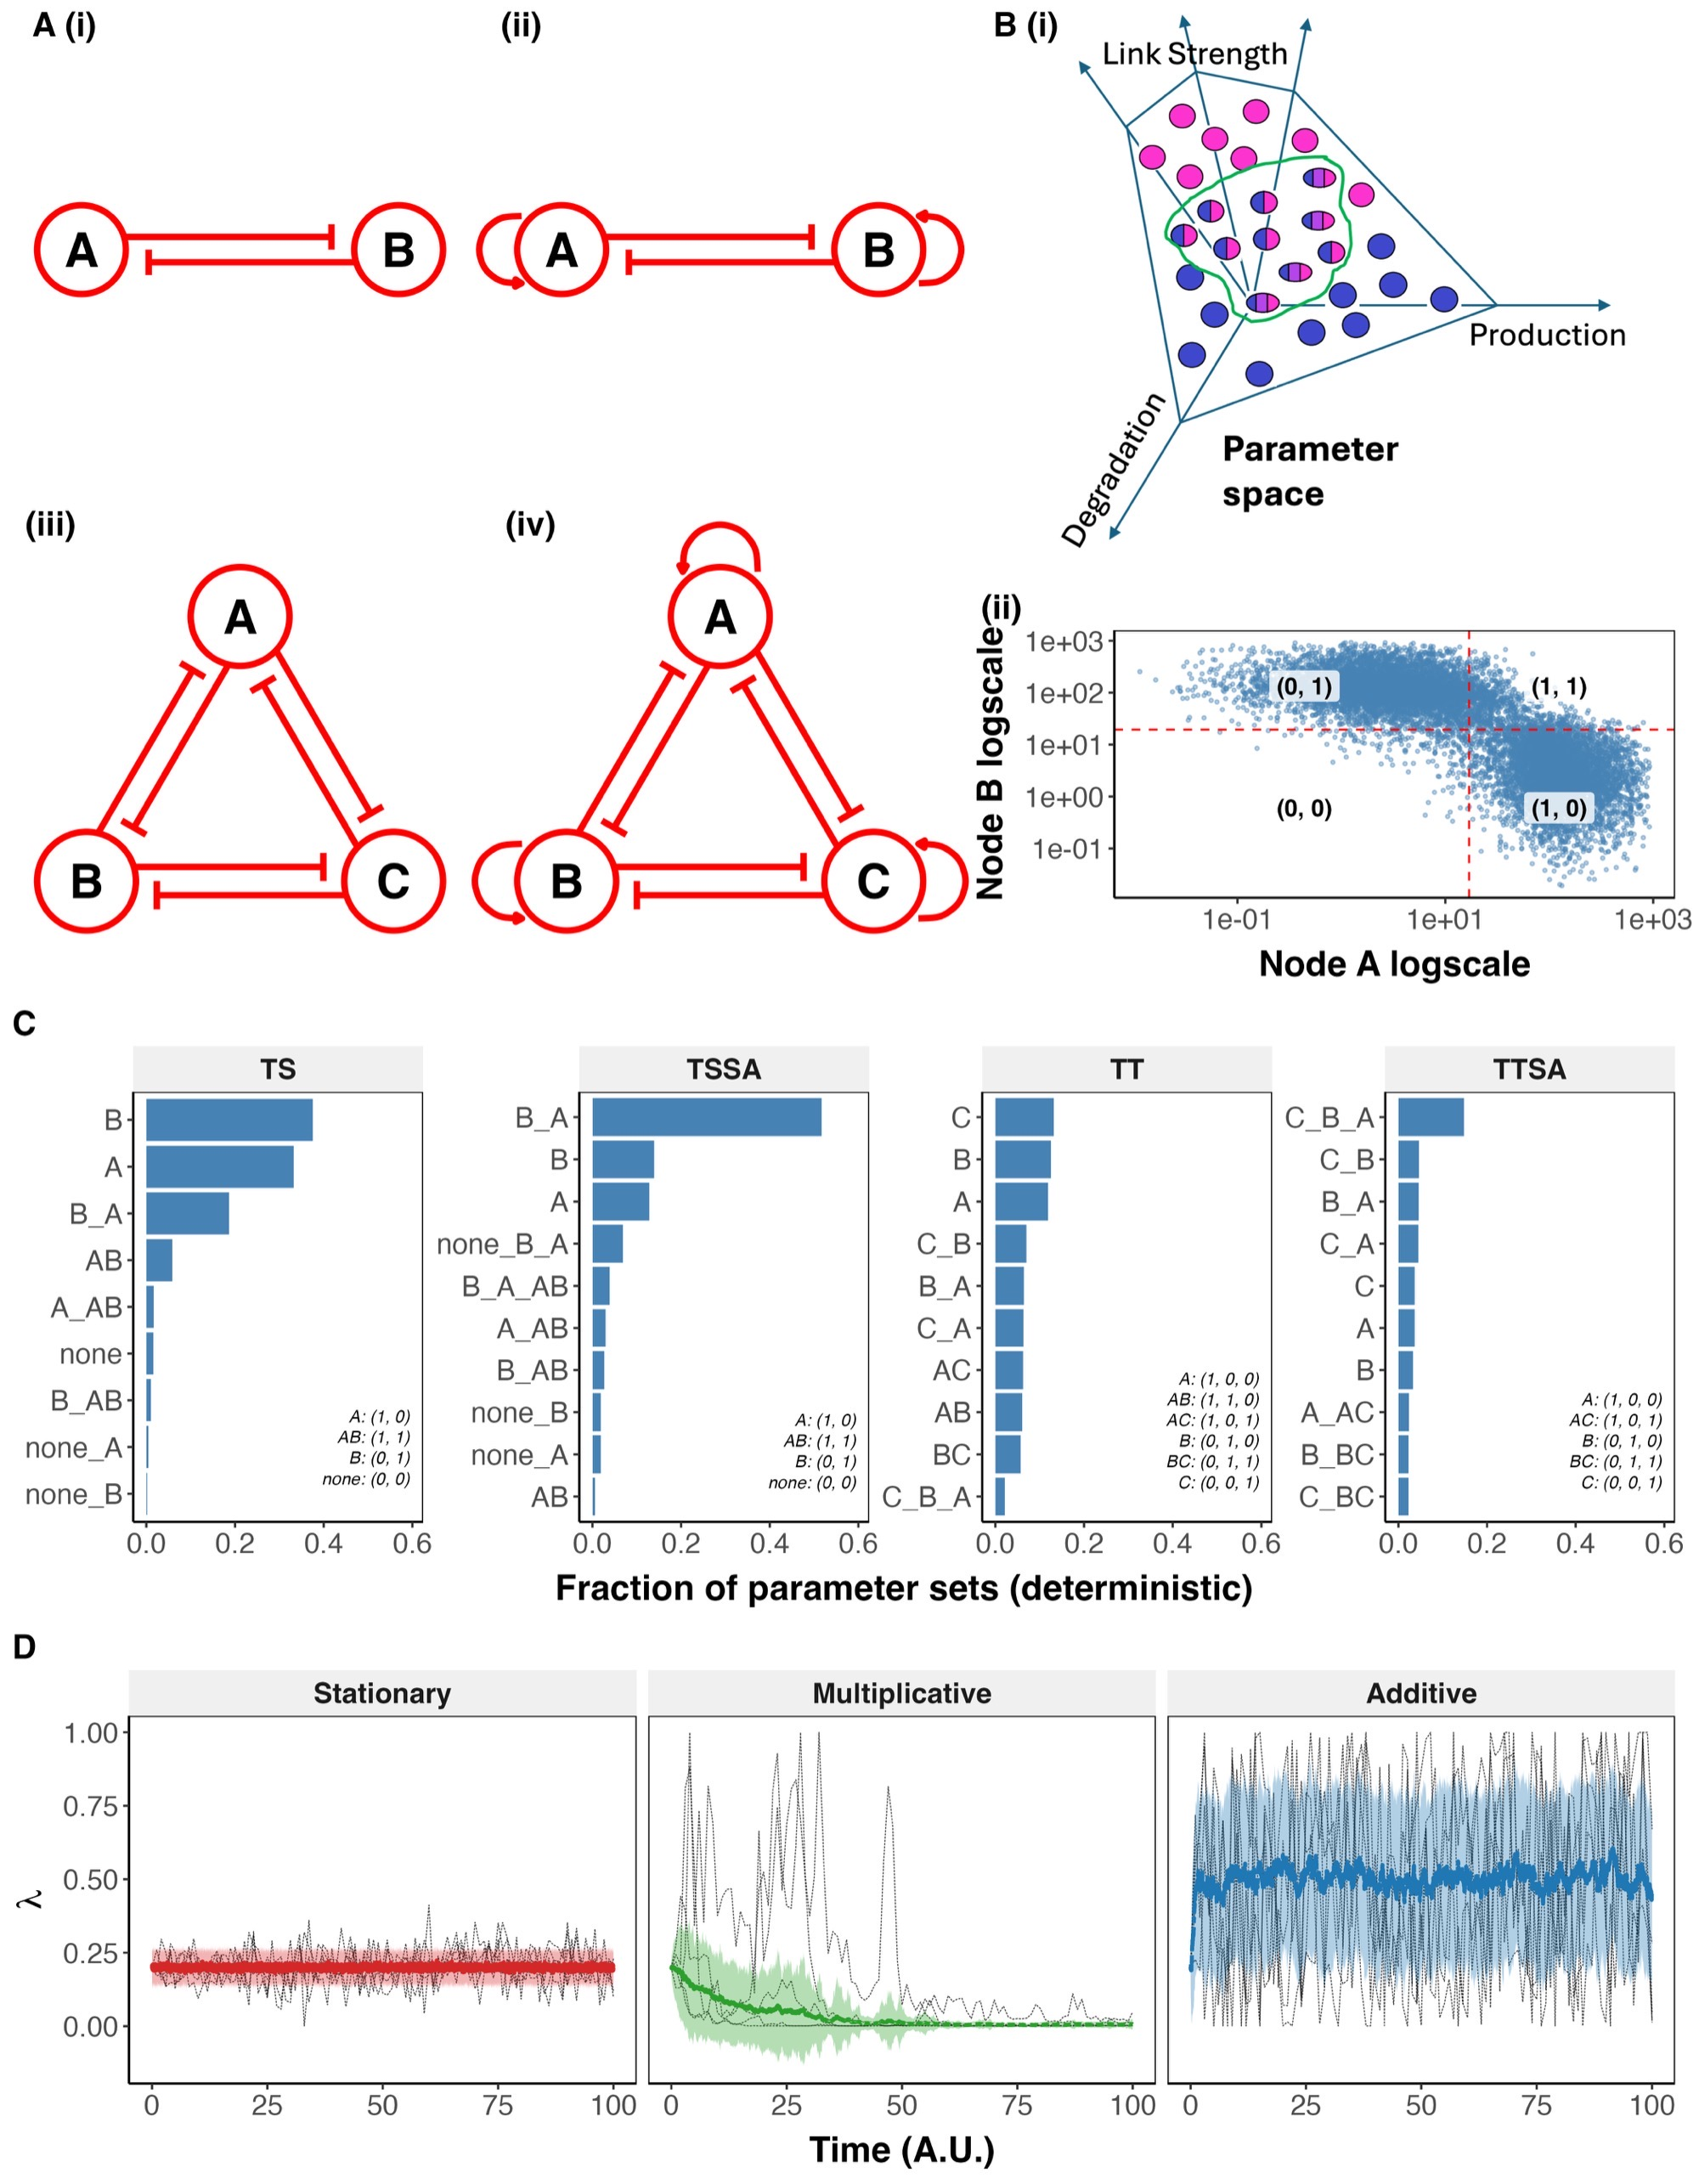
\includegraphics[width=0.8\linewidth]{Fig1.jpg}
    \caption{
    \textbf{RACIPE network topologies and the stochastic simulation framework.}. 
    \textbf{(A)} Network topology diagrams for the four base circuits used throughout this study: (i) TS (toggle switch), (ii) TSSA (toggle switch with self-activation), (iii) TT (toggle triad), (iv) TTSA (toggle triad with self-activation). Red circles denote nodes; bar-headed edges denote inhibitory interactions; curved arrows denote self-activation.
    \textbf{(B)} (i) Schematic of the RACIPE parameter-sampling framework: production, degradation, and interaction-strength parameters are randomly sampled within a bounded parameter space, generating an ensemble of models with varying dynamical behavior. (ii) Steady-state expression of node A vs. node B (log scale) across the RACIPE parameter ensemble for the TS network. Dashed red lines mark each gene's discretization threshold (mean of its expression in log scale across all steady states); quadrants are labeled with the corresponding discrete state, (A, B).
    \textbf{(C)} Frequency of the 10 most frequent discrete attractors found by RACIPE for each network (TS, TSSA, TT, TTSA), expressed as the fraction of parameter sets that map onto these attractors. States are represented in short-hand form, with the key given inside the plot. Compound labels (e.g.\ ``A\_B'') denote multistable parameter sets. Because TT and TTSA support many more distinct multistable combinations than TS/TSSA, the top-10 bars shown capture only part of the full ensemble: 100\%, 99.2\%, 77.5\%, and 46.2\% of all parameter sets for TS, TSSA, TT, and TTSA respectively (out of 9, 12, 97, and 119 total distinct attractor combinations found).
    \textbf{(D)} Simulated trajectories of the fold-change parameter $\lambda(t)$ under the three stochastic noise-update rules used in this study (Stationary, Multiplicative, Additive), shown for an inhibitory-edge-range parameter ($\lambda \in [0,1]$, $\lambda_0 = 0.2$). Thin black dashed lines show 5 representative individual trajectories (sampled once per time unit for legibility); the colored line and shaded ribbon show the mean $\pm$ SD across 100 simulated trajectories.}
    \label{fig:1}
\end{figure}

We begin by analyzing the binary and tertiary cell-fate decision motifs --- the toggle switch (TS) and the toggle triad (TT) and their extensions that include self-activation edges (TSSA and TTSA). A toggle switch consists of two mutually inhibiting transcription factors (Figure~\ref{fig:1}A(i-ii)), whereas a toggle triad consists of three mutually inhibiting transcription factors (Figure~\ref{fig:1}A(iii-iv)). TS represents the core motif underlying binary cell-fate decision networks. The phenotypic landscape emergent from TS is dominated by two states with mutually exclusive expression patterns - one of the nodes has low expression while the other is high - $(0,1)$ or $(1,0)$. Under appropriate parametric conditions, the toggle switch also exhibits bistability, enabling transitions between $(1,0)$ and $(0,1)$ states \cite{gardner2000construction}. The addition of self-activation (TSSA) stabilizes the $(1,1)$ state in which both nodes are co-expressed. This co-expression state, often referred to as a ``hybrid'' state, has been associated with stemness in development \cite{Roeder2006TowardsPU.1} and with high plasticity and pro-metastatic features in cancer \cite{jolly2015implications,jolly2018hybrid,Pastushenko2019EMTMetastasis}.

While binary cell-fate decision systems dominate biology owing to their stability and robustness to internal and external perturbations \cite{harlapur2022functional, Shyam2025MutuallyNetworks}, some instances of tertiary cell-fate systems --- such as T-cell differentiation --- employ a toggle triad architecture. A toggle triad consists of three mutually inhibiting transcription factors (Figure~\ref{fig:1}A(iii)) and permits three differentiated, single-high states where one of the three nodes has a high expression while the other two have low expression ($(0,0,1)$, $(1,0,0)$, and $(0,1,0)$) as well as three hybrid, double-high states with two out of three nodes having high expression (e.g.\ $(1,1,0)$). Parameter sweeps of the toggle triad result predominantly in monostable and bistable configurations, with a relatively smaller fraction exhibiting tristability. Single network architectures that allow the co-existence of four or more mutually exclusive states are not currently known~\cite{Bv2026GeneDecisions}.

We model these networks using a Hill-equation kinetics-based ODE system (Equation~\ref{eq:ode}, \ref{eq:hill}, Section~\ref{sec:RACIPE}). 
\begin{equation}
\frac{dX}{dt} = g_X \prod_{i \in P} \frac{H(Y_i, Y_{i0}, n_{Y_i}, \lambda_{Y_i})}{\lambda_{Y_i}} \prod_{i \in N} H(Y_i, Y_{i0}, n_{Y_i}, \lambda_{Y_i}) - d_X X
\label{eq:ode}
\end{equation}
\begin{equation}
H(Y_i, Y_{i0}, n_{Y_i}, \lambda_{Y_i}) = \lambda_{Y_i} \frac{Y_i^{\,n_{Y_i}}}{Y_{i0}^{\,n_{Y_i}} + Y_i^{\,n_{Y_i}}} + \frac{Y_{i0}^{\,n_{Y_i}}}{Y_{i0}^{\,n_{Y_i}} + Y_i^{\,n_{Y_i}}}
\label{eq:hill}
\end{equation}
Briefly, these equations combine transcription and translation into a single production term and a first-order degradation term representing mRNA and protein turnover. The production term consists of a rate constant ($g_X$) representing polymerization of RNA and protein, together with a combination of shifted Hill functions that formalize transcriptional regulation by input nodes. Input nodes change the production rate via the fold-change parameter $\lambda$: for inhibitory inputs, $\lambda < 1$, so that the presence of the regulator reduces the production rate; for activating inputs, $\lambda > 1$. The $\lambda$ of inhibitory links is bounded between 0.01 (strongest inhibition) and 1 (no inhibition) and that of the activating links is bounded between 100.0 (strongest activation) and 1.0 (no activation). 
%The shifted Hill functions are formulated such that the maximum production rate of any node is always $g_X$, making the maximum achievable expression $g_X/d_X$.  The fold-change parameter thus represents the regulatory efficacy of an input node, making it a natural target for studying structural stochasticity. 

We first simulated these networks deterministically using RACIPE~\cite{Huang2017}, a tool that allows us to explore the different configurations that the emergent phenotypic landscape can take across a large parameter space. RACIPE generates a large ensemble of ODE models by sampling multiple parameter sets (Figure~\ref{fig:1}B) and simulates each ODE model from multiple initial conditions until steady states are reached, resulting in an ensemble of steady states. We discretized expression of each node in each steady state into high (1) or low (0) based on the node's log-average expression across the ensemble of steady states (Figure~\ref{fig:1S1}B).  Threshold values for each network are given in Table~\ref{tb:Thresholds}. The models generated by RACIPE can be classified as monostable or bistable based on the number of discrete steady states they support, and further subdivided by the specific attractor configuration (see Table~\ref{tb:Attractors}). For the toggle switch, the dominant attractors were $(0,1)$, $(1,0)$, and the bistable $(0,1)\text{--}(1,0)$, as expected (Figure~\ref{fig:1}C, i). Although a small fraction of models do permit $(1,1)$ as a steady state, the corresponding fold-change parameters are always close to 1, rendering inhibitions ineffective~\cite{hari_assessing_2023}. TSSA enhances bistability in the parameter space, with the other dominant attractors being $(0,1)$ and $(1,0)$. Additionally, TSSA also supports tristability with $(0,1)$ and $(1,0)$ and either $(0, 0)$ or $(1, 1)$. The $(0, 0)$ state was accessed by a very small number of initial conditions, while $(1, 1)$ was more accessible (Figure~\ref{fig:1}C, ii). TT and TTSA support single-high (one of the nodes has a high expression - $(0, 0, 1)$ etc.) and double-high (two of the nodes have high expression - $(0, 1, 1)$ etc.) nearly equally. TTSA enhances multistability over TT, often exhibiting a tristable attractor with three single-high states (Figure~\ref{fig:1}C, iii, iv).

We explored three noise modes, described by the equations below: 
\begin{equation}
\begin{aligned}
\text{Additive:} \quad & \lambda(t+dt) = \lambda(t) + \mathcal{N}(0, \sigma_{\text{eff}}^2) \\
\text{Multiplicative:} \quad & \mu(t+dt) = \mu(t)\left(1 + \mathcal{N}(0, \sigma^2)\right) \\
\text{Stationary:} \quad & \lambda(t+dt) = \lambda(0) + \mathcal{N}(0, \sigma_{\text{eff}}^2) \\
\text{Where,} \quad & \sigma_{\text{eff}} = \sigma\lambda_{\text{max}}\text{;} \\
& \mu = \lambda \text{ for inhibitory edges, and } \mu = 1/\lambda \text{ for activatory edges}
\end{aligned}
\label{eq:lambda}
\end{equation}
Networks were simulated at eight levels of $\sigma$ : 0.0, 0.001, 0.005, 0.01, 0.05, 0.1, 0.5 and 1.0, scaled by the upper bound of $\lambda$ (Eq.~\ref{eq:lambda}, $\lambda_{max} = 1.0$ for inhibitory edges and $\lambda_{max} = 100.0$ for excitatory edges). The $\sigma$ values were chosen to ensure a larger coverage of the low to moderate noise region ($\sigma \leq 0.1$), as that region likely represents the underlying biology better than unrealistically high noises that span 50 or 100\% of the parameter range ($\sigma \in [0.5, 1.0]$). The higher $\sigma$ values serve a more theoretical purpose in helping us understand the effect of stochastic simulations. The three noise modes produce qualitatively distinct trajectories of $\lambda$ over time. Stationary noise models normally distributed fluctuations around the initial value of $\lambda$ (Figure~\ref{fig:1}D, \ref{fig:1S1}B). Additive noise models a constrained random walk of $\lambda$ bounded by the corresponding limits for activating and inhibiting $\lambda$ values. The resultant stationary distribution has a mean of 0.5 for inhibitory links and 50 for activatory links (Figure~\ref{fig:1}D, \ref{fig:1S1}B). Multiplicative noise makes each step proportional to the current value, which drives $\lambda$ toward its maximal-strength bound, where it stays (Figure~\ref{fig:1}D, \ref{fig:1S1}B). The consequences of these distinct $\lambda$ trajectories for network state dynamics are explored in the following sections.

% REVISION (R2.1): what lambda represents and what is not modeled.
The fold-change $\lambda$ is a phenomenological parameter for the effective strength of a regulatory interaction, and the three noise modes are generic stochastic processes for how that strength may vary in time. The model does not represent conformational states, post-translational modifications, chromatin or expression noise explicitly. The modes differ in two features that such processes can have: whether regulatory strength is anchored to a preferred value (stationary), wanders freely within bounds (additive) or strengthens progressively toward a maximum (multiplicative), and how fast it changes relative to gene expression.


We sampled monostable and bistable models separately from RACIPE, weighted by the relative frequencies of each attractor configuration. We then performed stochastic simulations of these networks by periodically perturbing $\lambda$. For each parameter set, we generated 100 stochastic trajectories starting from randomly chosen initial conditions. We use the RACIPE ensemble-derived thresholds (Figure~\ref{fig:1}B, ii, \ref{tb:Thresholds}) to discretize the stochastic trajectories as well. Based on the number of discretized steady states allowed by a given parameter set in the deterministic simulations, each parameter set was characterized as monostable (single steady state), bistable, tristable and so on. For each network, we sampled up to 1000 parameter sets per stability class (fewer where a stability class had fewer available parameter sets) and for each parameter set, we performed 100 stochastic simulations each to estimate the statistics.



\subsection{High levels of stationary noise pushes the system towards hybrid states}


\begin{figure}
    \centering
    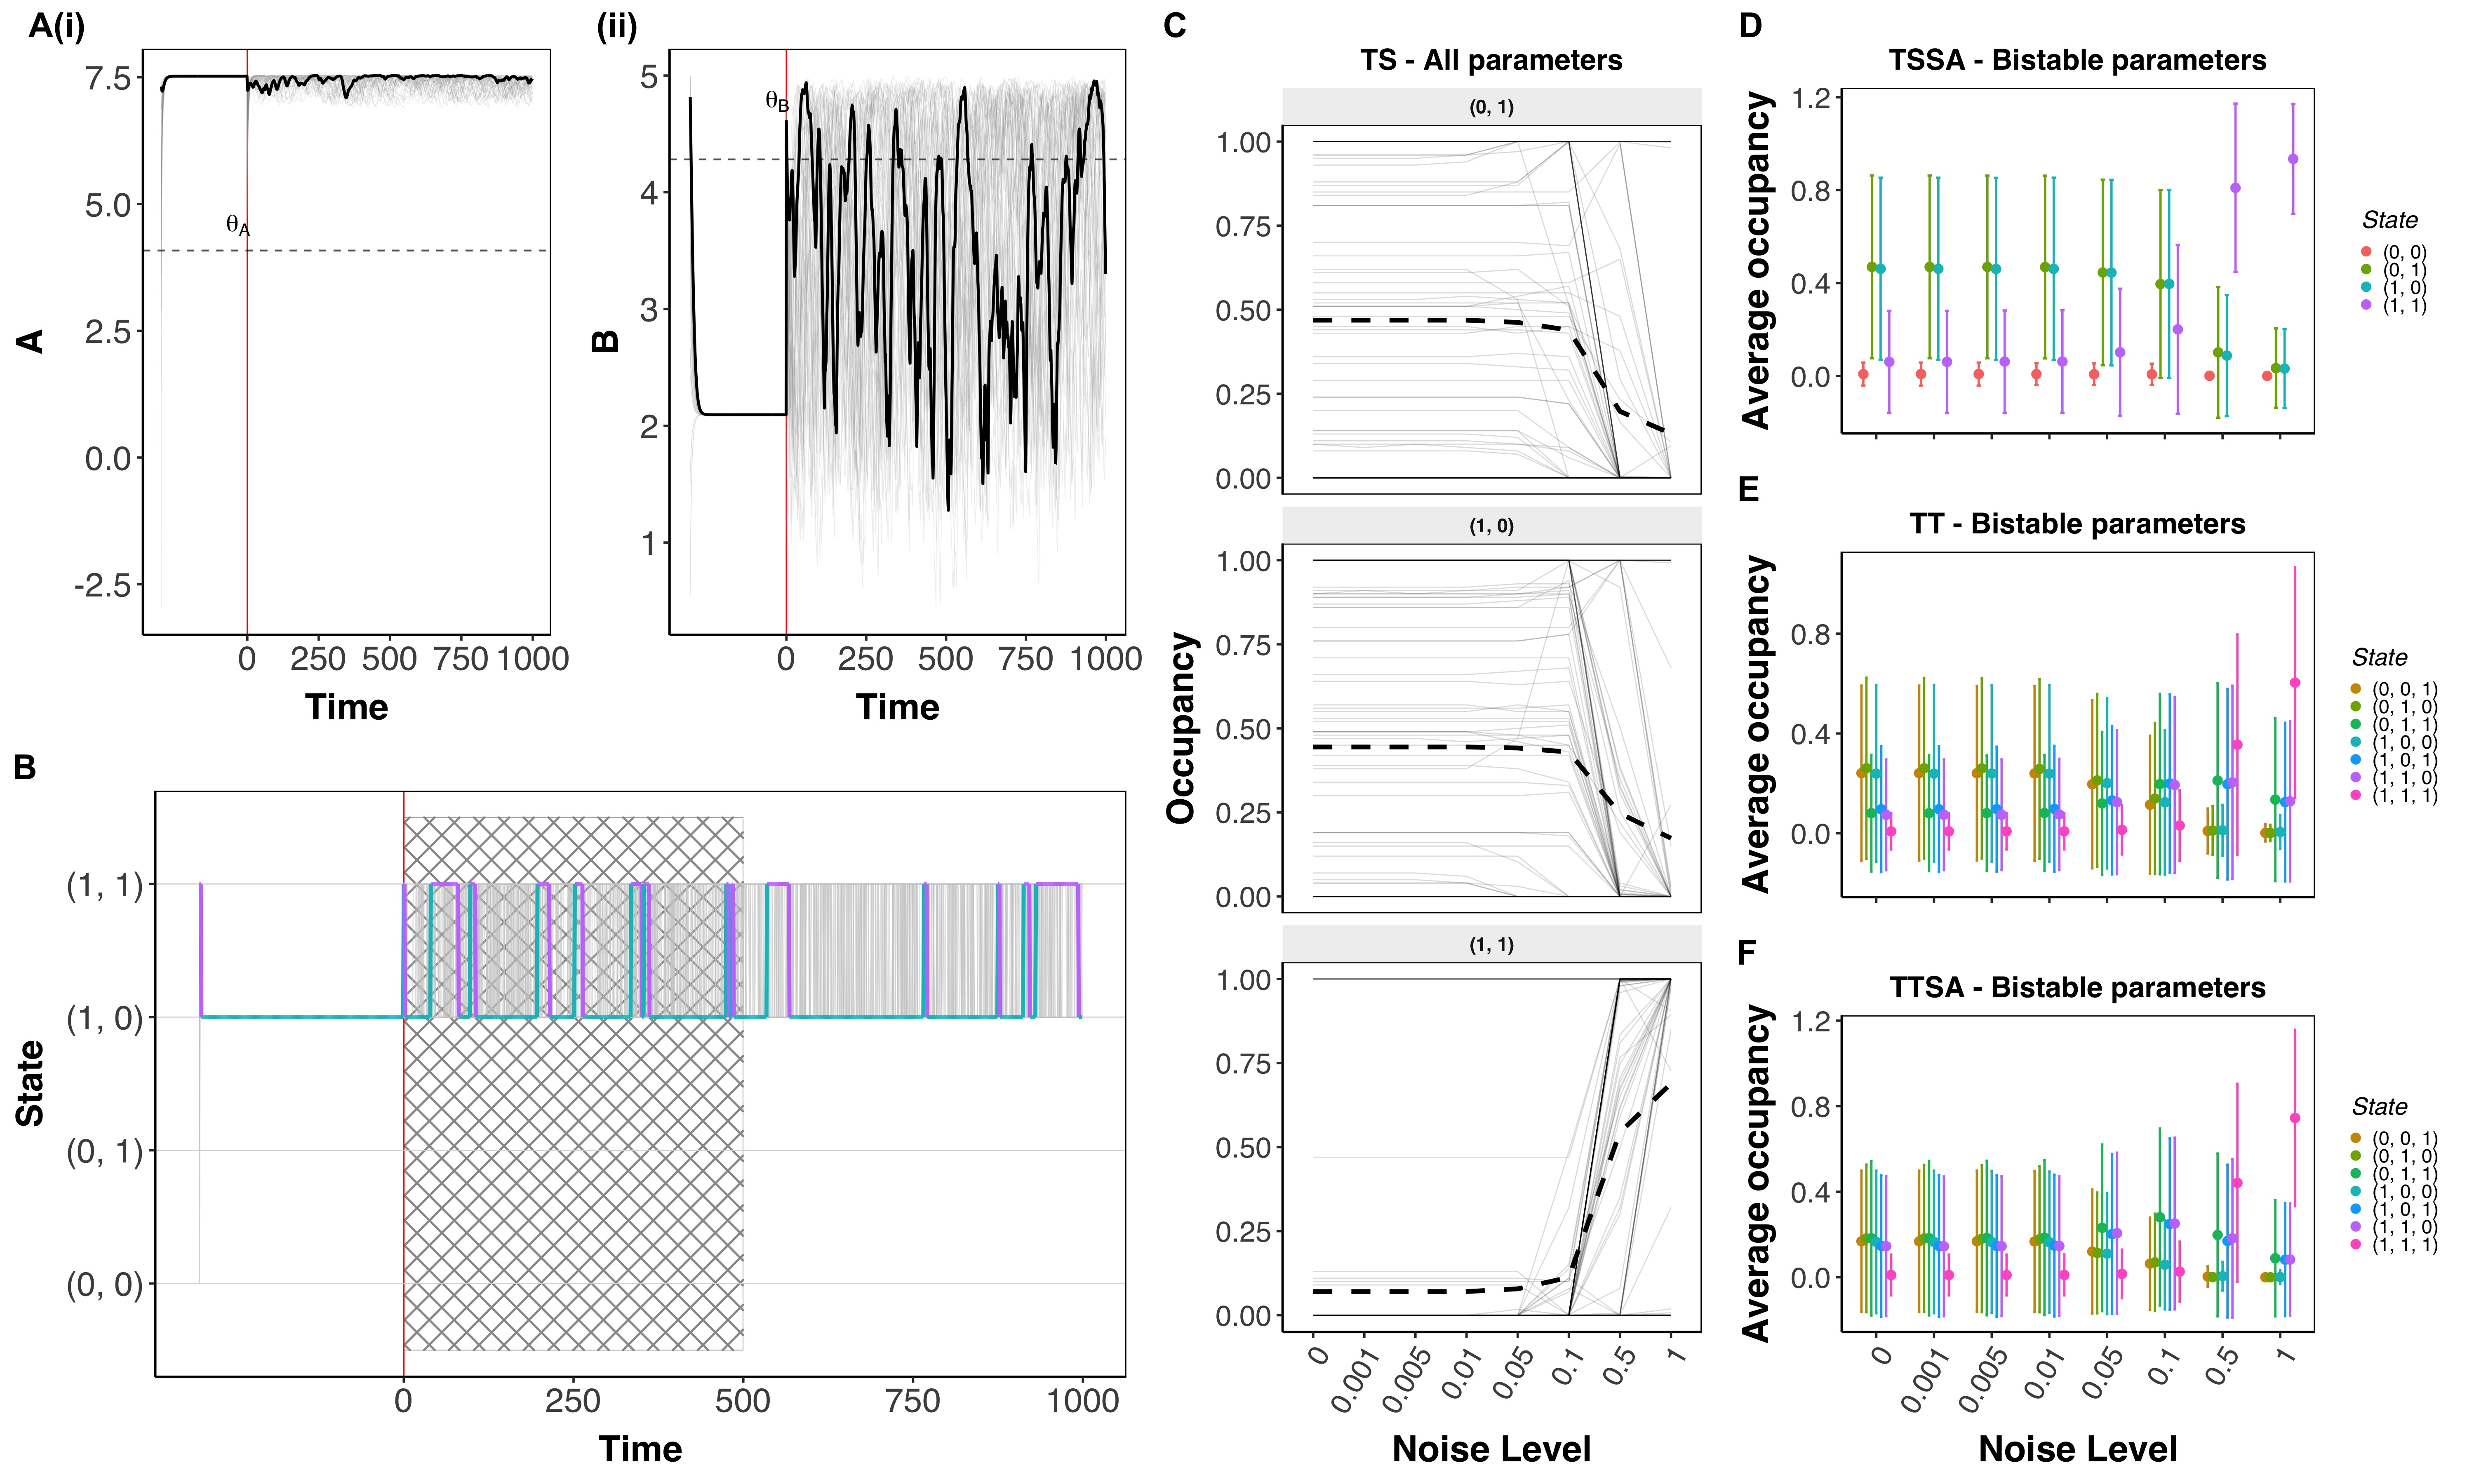
\includegraphics[width=\linewidth]{Fig2.jpg}
    \caption{\textbf{Effect of stationary noise on toggle switch and toggle triad networks}. 
    \textbf{(A)} Representative single-parameter trajectory for the TS network: (i) node A and (ii) node B expression over time (log$_2$), with the deterministic (noise-free) segment at negative time and the stochastic segment at positive time. Gray lines show all sampled initial conditions; the black line highlights one representative trajectory (the one whose switch count is closest to the population median); dashed horizontal line marks each node's discretization threshold $\theta$.
    \textbf{(B)} Discrete-state trace of the same parameter, colored by state for the highlighted trajectory (gray for all other initial conditions). Crosshatched region marks the discarded transient-dominated window of the stochastic segment. 
    \textbf{(C)} Occupancy of each state across noise levels. Each panel corresponds to the state indicated by its label. Grey lines show a random sample of 100 parameter-set trajectories (out of the full population, shown for legibility); the black dashed line shows the mean across the full parameter population, not just the sampled 100. Darker or apparently solid grey segments result from the overlap of multiple trajectories and do not denote a separate category.
    \textbf{(D--F)} Occupancy vs.\ noise level for TSSA (D), TT (E), and TTSA (F) bistable parameter sets, colored by state (top 4 states shown for TSSA, top 7 for TT/TTSA), mean $\pm$ SD across parameter sets. 
}
    \label{fig:2}
\end{figure}

Stationary noise mimics the classical assumption underlying GRN models, that the fitted parameters are the mean of a distribution whose variance does not significantly change the emergent phenotypic landscape from what the mean alone predicts. Thus, we started with analyzing the stochastic simulations under stationary noise to evaluate the validity of the deterministic representation of regulatory parameters. We analyzed the stochastic trajectories by first discretizing them using the RACIPE ensemble threshold values (Figure~\ref{fig:2}A). The resultant discrete state trajectories are then used to calculate the occupancy of each state, the fraction of time steps a trajectory spends in that state averaged over the 100 trajectories of a parameter set (Methods), which we use to evaluate the occurrence of a state for a given parameter set under a given noise type and noise level (Figure~\ref{fig:2}B). Note that we use the same occupancy calculation for deterministic simulations here on (e.g., $\sigma = 0$). As deterministic simulations reach steady state by the burnin period (shaded in criss-crossed lines in Figure~\ref{fig:2}B), occupancy measures the relative size of the basin of attraction. For monostable parameters, the occupancy in deterministic simulations is always 1, while multistable parameters have fractional occupancy corresponding to the basin size of the specific steady state in the attractor. 

As expected, the dominant states for a toggle switch remain as $(0, 1)$ and $(1, 0)$ for low to moderate $\sigma$ values under stationary noise. However, as the $\sigma$ increases to 0.5 and above (i.e., the noise scales as 50\% of the allowed range of $\lambda$), we see a drop in the occupancy of the (0,1) and (1, 0) states and a corresponding increase in the occupancy of the (1, 1) state - which represents a co-expression of both nodes that normally inhibit each other (Figure~\ref{fig:2}C). Note that a similar increase is not seen in the occupancy of the (0, 0) state (Figure~\ref{fig:2S1}A), an asymmetric outcome despite the symmetry of the stationary noise. We further studied TSSA, TT and TTSA under stationary noise and found them behaving similarly. TSSA, in absence of noise enables bistability in a larger fraction of parameter space than TS ($\approx 20\%$ in TS vs $>50\%$ in TSSA). TSSA also enables $\approx$14\% of the state space to be tristable, with access to either $(0, 0)$ or $(1, 1)$ state in addition to the dominant $(0, 1)$ and $(1, 0)$ states. However, the basin size of $(0, 0)$ state, is negligibly small, making $(0, 1) - (1, 0)-(1, 1)$ the only real tristable configuration (Figure~\ref{fig:2S1}B - tristable parameters at $\sigma = 0$). Similar to TS, TSSA maintains the characteristics of its phenotypic landscape under stationary noise - dominant $(0,1)$ and $(1,0)$ states in monostable and bistable parameter sets, and dominant $(1, 1)$ state in tristable parameter sets for realistic values of noise, i.e., $\sigma \leq 0.1$ (Figure~\ref{fig:2}D). For higher $\sigma$, we see a dominance of the $(1, 1)$ state. 

Toggle triad (TT) and toggle triad with self-activation (TTSA) dominantly enable two classes of steady states - single-high states ($(0, 0, 1); (0, 1, 0)$ and $(1, 0, 0)$ and double-high states ($(0, 1, 1); (1, 0, 1) and (1, 1, 0)$). Previous studies have shown that the toggle triad motif is more susceptible to various perturbations due to the inherent frustration in the network~\cite{harlapur2022functional, doi:10.1098/rsif.2020.0631}. Here, we see that the occupancy distribution of TT starts to change for $\sigma > 0.01$, showing a higher sensitivity to noise than TS and TSSA motifs (Figure~\ref{fig:2}E, F, Figure~\ref{fig:2S1}C-D). At $0.01 \leq \sigma \leq 0.1$, the occupancy of single-high states starts to go down and that of double-high states starts to come up, still qualitatively retaining the properties of the phenotypic landscape. However, $\sigma \geq 0.5$ leads to an increase in the occupancy of the all-high state ($(1, 1, 1)$) in both TT and TTSA, similar to that of TS and TSSA, with no emergence of the all-low state ($(0, 0, 0)$). Overall, we find that the phenotypic landscape of both binary and tertiary cell-fate GRNs remains robust to stationary noise of low to moderate levels of $\sigma$. The response to larger noise can be better understood based on our analysis of additive noise given in the next section. 


\subsection{Additive noise reshapes the phenotypic landscape toward high-expression states, modulated by reachability and threshold margin}

Unlike stationary noise, additive noise starts to change the phenotypic landscape even at low $\sigma$ values. For the toggle switch across a majority of the parameters, we see a decrease in the occupancy of single-high states ($(0, 1)$ and $(1, 0)$) and an increase in the hybrid all-high ($(1, 1)$) state occupancy (Figure~\ref{fig:3}A). The mean occupancy of all-high state crosses 0.5 for $\sigma > 0.001$ (0.1\% of the $\lambda$ range) and stabilizes at 0.75 for $\sigma > 0.1$. Given the biological relevance of hybrid states showing co-expression of all nodes in developmental and pathological contexts, this shift in the phenotypic landscape of cell-fate decision motifs is a very significant finding. 

\begin{figure}
    \centering
    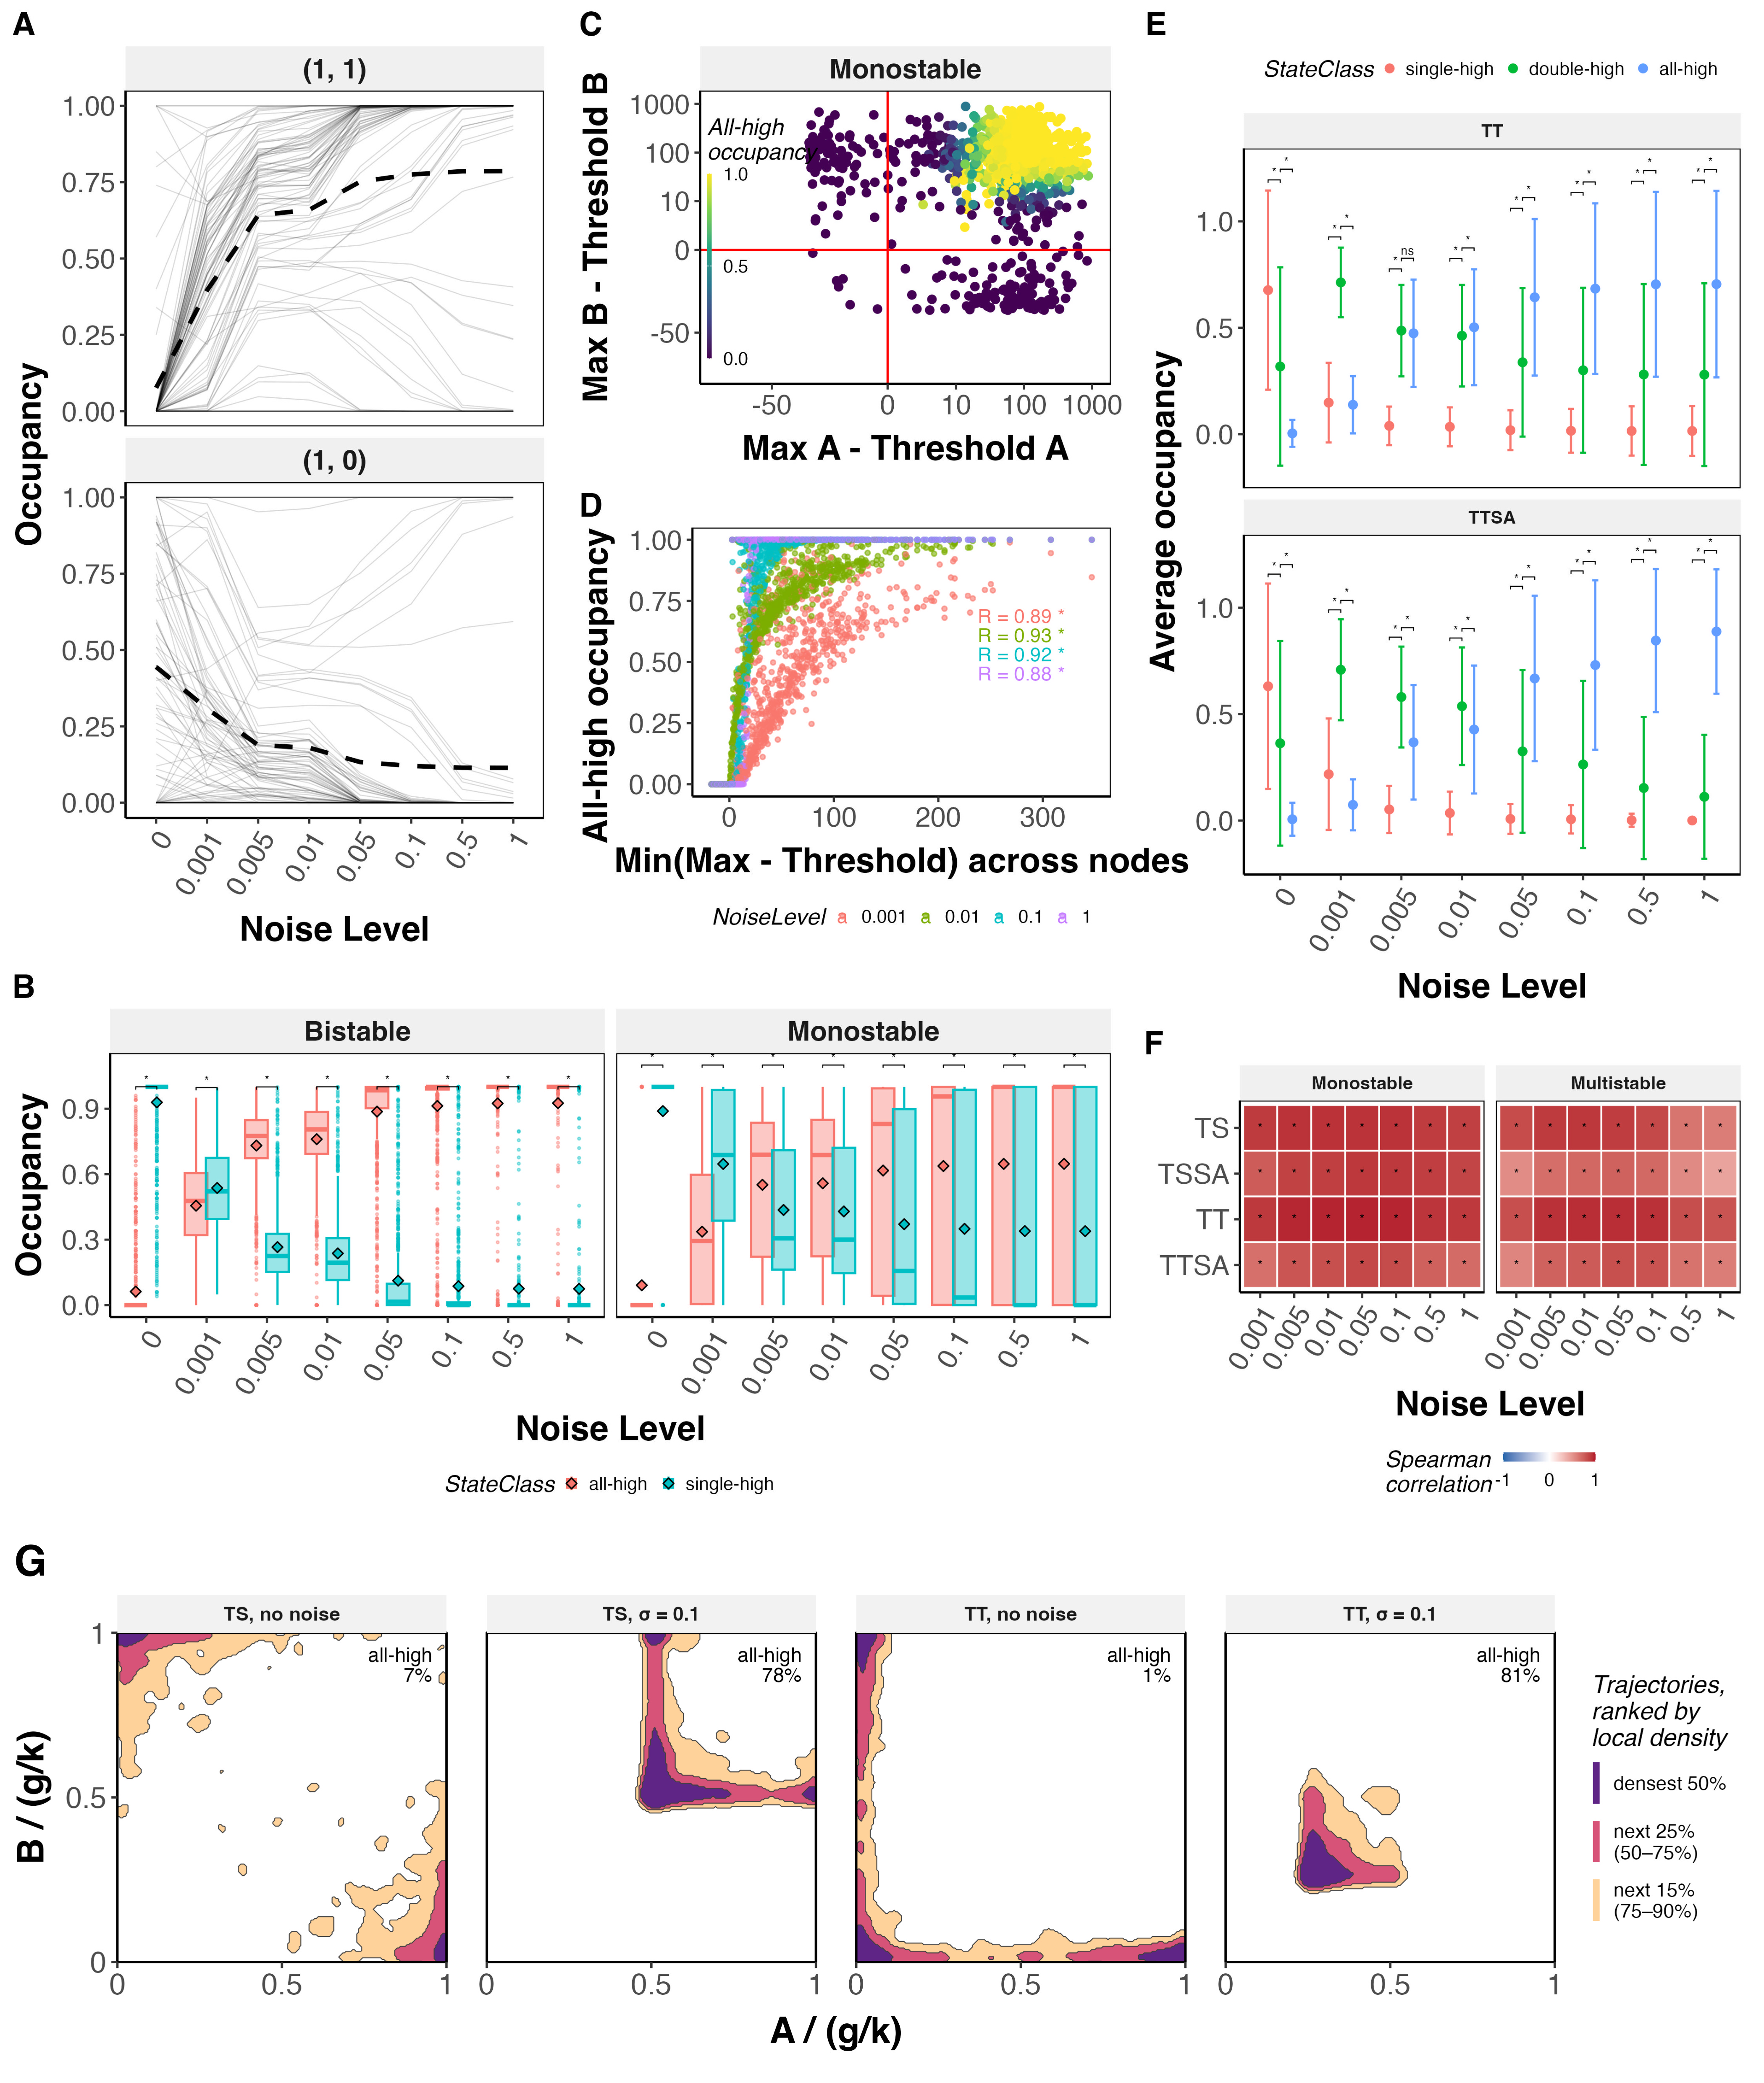
\includegraphics[width=0.85\linewidth]{Fig3.jpg}
    \caption{\textbf{Effect of Additive noise on the phenotypic landscape of cell-fate decision networks}
    \textbf{(A)} Occupancy of $(1, 1)$ and $(1, 0)$ states vs.\ noise level for the TS network, a random sample of 100 parameter-set trajectories (gray) with the mean across the full parameter population (dashed).
    \textbf{(B)} Occupancy boxplots for the TS network, monostable vs.\ bistable parameter sets, all-high vs.\ single-high states, with paired Wilcoxon significance brackets; ``*'' $p-value<0.05$, ``ns'' not significant. 
    \textbf{(C)} Reachability scatter for TS monostable parameter sets at $\sigma = 0.1$: each node's (max expression $-$ threshold) margin on the x/y axes, colored by occupancy of the (1,1) state.
    \textbf{(D)} Spearman correlation between the minimum reachability margin across nodes and occupancy of the (1,1) state, across four noise levels (0.001, 0.01, 0.1, 1), TS monostable parameter sets.
    \textbf{(E)} Occupancy vs.\ noise level for TT and TTSA, single-high $\to$ double-high $\to$ all-high state classes shown as Mean $\pm$ SD across all parameters, with paired Wilcoxon significance brackets between adjacent classes; ``*'' $p-value<0.05$, ``ns'' not significant. 
    \textbf{(F)} Heatmap of the Spearman correlation between minimum reachability margin and occupancy of the all-high state, across networks (TS, TSSA, TT, TTSA), noise levels, and stability class (monostable vs.\ multistable); ``*'' $p-value<0.05$, ``ns'' not significant.
    \textbf{(G)} Joint time-averaged expression of nodes A and B per trajectory, as a fraction of each parameter set's maximum ($g/k$), for TS and TT without noise (C0) and under additive noise ($\sigma = 0.1$, $\Delta t = 0.01$; 2,000 TS and 2,568 TT parameter sets $\times$ 100 trajectories). For TT, node C is not shown. Colours rank trajectories by local density: the darkest region is the smallest area holding 50\% of trajectories, and the next two bands add 25\% and 15\% (highest-density regions of a two-dimensional kernel density estimate). Dashed lines: the ensemble discretization thresholds of A and B in units of $g/k$. Each threshold is a single absolute value, so in these units it differs between parameter sets; the line is the median over parameter sets and the grey band the interquartile range. Numbers give the fraction of trajectories in each quadrant, using each parameter set's own threshold, so trajectories above the median line can still be classified low. For TT, the all-high fraction (A, B and C high) is also given. All networks and $\sigma$ values are shown in Figure~\ref{fig:3S_expr}.
}
    \label{fig:3}
\end{figure}

Interestingly, we note that while most parameters gravitate towards a high occupancy for the all-high state for $\sigma \geq 0.01$, a smaller fraction of the parameters also show a significantly lower occupancy of all-high state (Figure~\ref{fig:3}A). When we separately studied the parameter sets based on their multistability characteristics under deterministic dynamics, we found that monostable states always had a lower occupancy for all-high states under additive noise as compared to that of multistable parameter sets (Figure~\ref{fig:3}B). Given how readily bistable parameters converge to the all-high state, we hypothesized that the reduced occupancy for monostable states could possibly arise because the all-high state is not accessible to some monostable parameter sets.  The upper limit of node expression in the ODE models we simulated is the ratio of the corresponding production and degradation rates. As we use a threshold derived from the ensemble steady state expression levels, it is possible that some parameter sets are sampled such that the upper limit of expression for one of the nodes defined by the production and degradation rates is lower than the threshold. Since the bistable parameters consist of two single-high states, bistable parameter sets never have this shortcoming. 

Thus, we wanted to understand whether it really is the case that some of the sampled monostable parameters reflect systems that cannot access the all-high state and in turn, if the access to all-high state is sufficient for the additive noise to push the system towards all-high state. To do this, we plotted the sampled parameter sets on the axes of ``reachability'' defined by the difference between the upper limit of a node's expression level and the threshold used to discretize that node. Reachability was not satisfied for all sampled parameters: for the TS network, 89.0\% of parameter sets had a production/degradation-derived expression ceiling exceeding threshold for both nodes, 10.8\% reached threshold for only one of the two nodes, and 0.3\% reached threshold for neither; among monostable parameter sets specifically, those that are not reachable for both nodes correspondingly show an occupancy of exactly 0 for the all-high state, confirming that unreachable parameter sets are the origin of the low-occupancy tail seen in the monostable population (Figure~\ref{fig:3}C, \ref{fig:3S1}A). Among the reachable parameter sets, however, we see that the occupancy of the all-high state increases with increasing distance between the maximum allowed value of the nodes and the corresponding thresholds. Across $\sigma$ values, the occupancy of the all-high state correlated strongly positively with the smallest of the two difference values (Figure~\ref{fig:3}D).

TSSA showed a similar increase in hybrid (all-high) state occupancy under additive noise. At low to moderate $\sigma$, TS and TSSA showed very similar occupancy distributions. At high $\sigma$ values, TSSA monostable parameter sets showed a higher occupancy of all-high states compared to TS (Figure~\ref{fig:3S1}B, i). This increase can be attributed to the inherent affinity TSSA has towards all-high state as discussed earlier. For TT and TTSA, we observed a transition of states from single-high to double-high to all-high, suggesting that while additive noise does push the system towards the all-high state, the transformation can become more gradual as the network size increases (Figure~\ref{fig:3}E, \ref{fig:3S1}B, ii, iii). TT and TTSA have similar occupancy distributions for low to moderate values of $\sigma$, with similar average occupancy of all-high and double-high states. But at high values of $\sigma$, TTSA showed a higher occupancy of the all-high state, with the double-high state average occupancy approaching 0. TT on the other hand maintains a non-zero average occupancy of double-high states even at higher $\sigma$ values (average occupancy across all parameter sets - all-high 0.7 vs double-high 0.3 for TT vs all-high 0.9 and double-high 0.15 for TTSA). For all networks, we found a strong positive correlation between the difference quantity (max node expression minus threshold expression of the node) and the occupancy of all-high states in monostable parameter sets. Multistable parameter sets showed relatively weaker correlations (Figure~\ref{fig:3}F). Overall, our analysis clearly shows that additive noise increases the occupancy of hybrid, all-high states in cell-fate decision networks. 

% REVISION (R3.7): expression levels behind the all-high label; production run 2026-10-csbj-v2, CSBJ_review/fig3_expression.
Because the discretization thresholds come from the deterministic ensemble, a trajectory classified as all-high need not have its nodes near their maximum expression. We therefore examined the time-averaged expression of each node as a fraction of its parameter-set-specific maximum, $g/k$ (Figure~\ref{fig:3}G, \ref{fig:3S_expr}). Without noise, TS and TT trajectories sit near the single-high corners: the high node is close to its maximum and the repressed node close to zero. Under additive noise both nodes are expressed together, but below their maximum. For $\sigma \geq 0.1$ the TS distribution has a sharp lower edge at half of the maximum. This edge is the floor set by weakened repression: the production of a repressed node cannot fall below $\lambda$ times its maximum, and the time-averaged $\lambda$ of every TS edge is 0.505, the mean of the clipped random walk, which is uniform on $[0.01, 1]$. About 70\% of node expression values lie within 1.25-fold of this floor. In TT each node has two repressors, and the floor drops to about $\lambda^2 \approx 0.25$. Relative to each parameter set's own noise-free states, the median node under noise ($\sigma = 0.1$) is 1.6-fold below its noise-free high level and 18-fold above its noise-free repressed level in TS, and 2.4-fold below and 29-fold above in TT. The ensemble thresholds lie below the floor in most parameter sets (Figure~\ref{fig:3}G), so these trajectories are classified as all-high (78\% in TS, 81\% in TT). At $\sigma = 0.01$ the distribution is broader because $\lambda$ changes slowly enough for expression to follow it (Figure~\ref{fig:3S_expr}). The all-high state produced by additive noise is therefore sustained co-expression at sub-maximal levels, with each node repressed down to the floor set by the average fold change, rather than simultaneous maximal expression. Whether such co-expression corresponds to a functional hybrid phenotype, or to transient imbalance, depends on the biological system.

\subsection{Increased occupancy of all-high states is caused by both the $\lambda$ distribution and stochasticity}

Following the strong correlation we observed between parametrically determined upper bounds of node expression and the occupancy of all-high state, we hypothesized that the drastic increase in the occupancy of all-high states in comparison to deterministic simulations might also be explained by variation in the parameter space. Additive noise models a random walk in $\lambda$, bounded between 0.01 and 1 for inhibitory links and 1 and 100 for activating links. A step that would cross a bound sets $\lambda$ to that bound; for example, if $\lambda(t) + \eta(t) < 0.01$ then $\lambda(t+dt) = 0.01$. The bounds are not absorbing: later steps can move $\lambda$ back into the interior. Due to the nature of random walk, the variance of $\lambda$ increases over time, unlike the stationary noise case. Furthermore, this clipping increases the chances of $\lambda$ being at either of the borders than in the interior. The probability density of $\lambda$ at the borders increases with increasing $\sigma$, as at larger $\sigma$ values, there is a higher chance of taking larger $\lambda$ steps and correspondingly higher chances of hitting the boundaries (Figure~\ref{fig:3b}A). Same boundary conditions are applied to other noise forms as well, and we see such boundary behavior in stationary noise at high $\sigma$, where $\lambda$ localizes at either of the boundaries. While $\lambda$ closer to zero leads to a very strong inhibition by drastically reducing the net production rate, $\lambda$ closer to 1 leads to very weak inhibition and lets the production rate reach the highest values. Despite this symmetry in the emergent $\lambda$ distribution, the shift in the landscape is asymmetric towards all-high states. One potential reason could be the way the $\lambda$ parameter is sampled in RACIPE for inhibitory interactions. The fold-change parameter is first sampled between 1 and 100 and then the inverse of that number is used for inhibitory links. Thus the distribution of $\lambda$ for inhibitory links is tailed heavily towards lower values of $\lambda$ with a mean of $\approx0.05$. As the stationary distribution of $\lambda$ in additive noise has a mean of 0.5, as a simulation progresses the inhibitory links experience a significant increase in the average $\lambda$, which in turn leads to weakening of the inhibition.

% REVISION (R1 minor 2, R3.5): frozen-lambda control with 1,000 draws from each set's own trajectories; production run 2026-10-csbj-v2.
Given the above, we wanted to know if this shift in $\lambda$ distribution is enough to explain the increase in the occupancy of all-high states. For each parameter set we drew 1{,}000 vectors of fold-changes from the values visited by that set's own stochastic trajectories and simulated each deterministically from one of the 100 initial conditions (frozen-$\lambda$ control, C4; Section~\ref{sec:controls}). The original RACIPE parameters of TS give a non-zero all-high frequency for only a small fraction of parameter sets, but with frozen draws from the noise-induced distribution all-high occupancy increases for 81--83\% of parameter sets, by 0.55 on average at $\sigma = 0.01$ and by 0.34 at $\sigma = 1$ (Figure~\ref{fig:3b}B, left). The same holds for TT, TSSA and TTSA (Figure~\ref{fig:3bS1}A). Thus, the change in the $\lambda$ distribution alone accounts for most of the increase in the occupancy of the all-high state. This might be relevant if a GRN is subjected to the onset of regulatory noise due to its interaction with some additional dynamical factor.

Time variation of $\lambda$ adds to this shift, but only once the noise is fast enough. The stochastic effect, the difference between the stochastic occupancy (C1) and the frozen-$\lambda$ occupancy (C4) of the same parameter set, is close to zero for $\sigma \leq 0.01$ (TS: $+0.004$, $+0.012$ and $+0.03$ at $\sigma = 0.001$, 0.005 and 0.01) and grows to $+0.18$ at $\sigma = 0.1$ and $+0.38$ at $\sigma = 1$ (Figure~\ref{fig:3b}B, right; other networks in Figure~\ref{fig:3bS1}B). At low noise $\lambda$ changes slowly and the stochastic simulation behaves like frozen heterogeneity. Across parameter sets, the stochastic and frozen-$\lambda$ occupancies follow a sigmoidal relationship (Figure~\ref{fig:3b}C; TS, $\sigma = 0.1$, Spearman $\rho = 0.90$): parameter sets whose frozen-$\lambda$ occupancy of the all-high state is below $\approx 0.5$ lose all-high occupancy under noise, whereas those above it approach an occupancy of 1 (78\% of parameter sets lie above the diagonal). Figure~\ref{fig:3b}D places these comparisons in the full sequence of controls for TS, and Figure~\ref{fig:3b}E summarizes the decomposition for all seven networks; both are discussed in Section~\ref{sec:timescale}. Increasing the update interval $dt$ of the noise process from 0.01 to 1 and 10 (C2) lowers the occupancy of the all-high state toward the frozen level (Figure~\ref{fig:3b}D), because expression has time to relax toward the landscape set by each value of $\lambda$. These results indicate that, while the distribution of $\lambda$ shifts the landscape toward the all-high state, time variation of $\lambda$ enhances this shift when it is fast relative to expression relaxation.

\begin{figure}
    \centering
    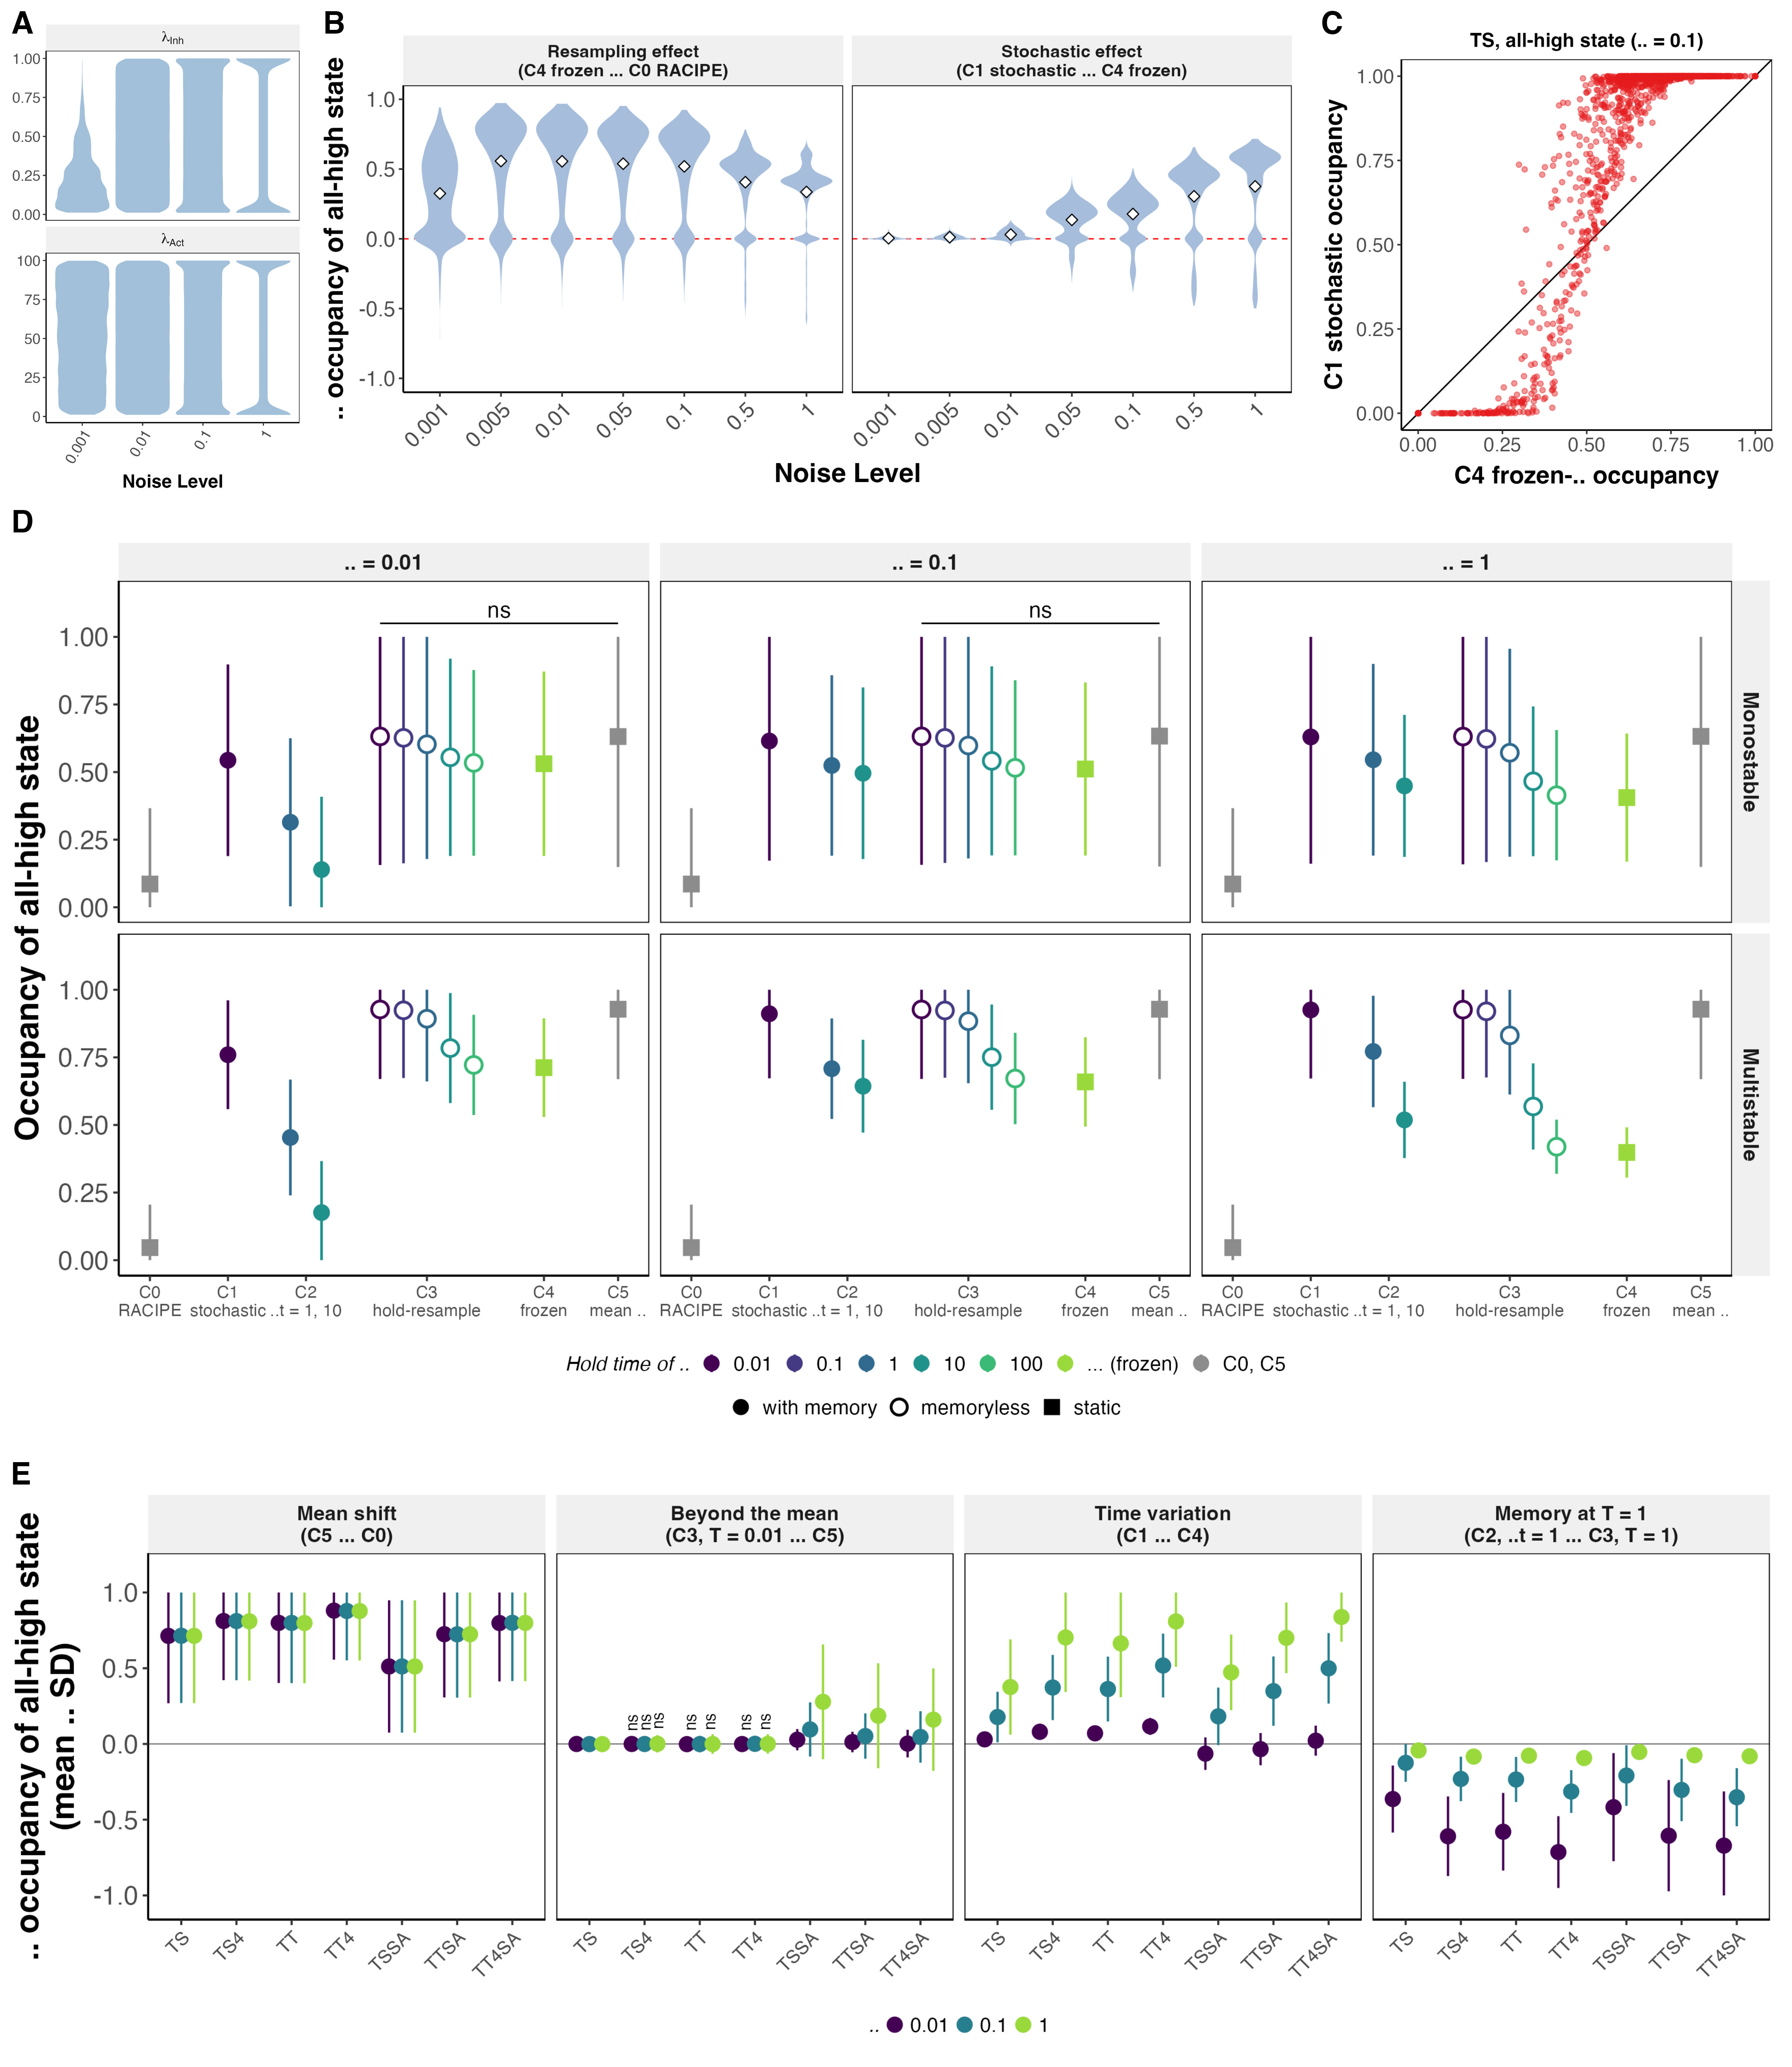
\includegraphics[width=0.9\linewidth]{Fig4.jpg}
    \caption{\textbf{The additive noise effect combines a shift in the $\lambda$ distribution with a contribution from time variation of $\lambda$.} Additive noise, $dt = 0.01$ unless stated.
    \textbf{(A)} Distribution of the regulatory fold-change $\lambda$ visited during the stochastic simulations, for (i) inhibitory and (ii) activating edges, at four noise levels.
    \textbf{(B)} TS: per-parameter-set resampling effect (frozen-$\lambda$ occupancy, C4, minus original RACIPE occupancy, C0) and stochastic effect (stochastic occupancy, C1, minus C4) of the all-high state, at every noise level. Diamonds, means; violins, distribution over 2{,}000 parameter sets. C4 uses 1{,}000 frozen draws per parameter set from that set's own stochastic trajectories.
    \textbf{(C)} TS, $\sigma = 0.1$: frozen-$\lambda$ versus stochastic occupancy of the all-high state; each point is a parameter set and the line is the diagonal.
    \textbf{(D)} TS: Occupancy of the all-high state (mean $\pm$ SD over parameter sets) across the sequence of controls, for monostable and multistable parameter sets (rows) at $\sigma = 0.01$, 0.1 and 1 (columns). C0, original RACIPE parameters; C1, stochastic simulation; C2, stochastic simulation with update interval $dt = 1$ and 10; C3, $\lambda$ drawn independently from the visited distribution and held for $T_\text{hold} = 0.01$--100 (memoryless); C4, frozen $\lambda$; C5, every edge fixed at its mean $\lambda$. Colour, time for which a value of $\lambda$ persists; filled symbols, noise process with memory; open symbols, memoryless resampling. Paired Wilcoxon tests between adjacent conditions and between C2 and C3 at equal hold time, Benjamini--Hochberg corrected; only non-significant pairs (ns, adjusted $p \geq 0.05$) are marked.
    \textbf{(E)} Decomposition for all seven networks (mean $\pm$ SD over parameter sets of the per-set difference in all-high occupancy): change in mean regulatory strength (C5 $-$ C0), effect of fast fluctuations beyond the mean (C3 at $T_\text{hold} = 0.01$ $-$ C5), effect of time variation (C1 $-$ C4), and effect of memory at a hold time of 1 (C2 at $dt = 1$ $-$ C3 at $T_\text{hold} = 1$; at $\sigma = 0.01$ this also includes the narrower $\lambda$ distribution reached at long $dt$). ns, one-sample Wilcoxon test, Benjamini--Hochberg adjusted $p \geq 0.05$. Production run, up to 1{,}000 parameter sets per stability class.}
    \label{fig:3b}
\end{figure}


% REVISION (R1.5): asymmetry stated as regulator dependence; two-boundary analysis moved to the Supplementary (Section~\ref{sec:asymmetry}). Production run 2026-10-csbj-v2, dt = 0.01.
The effect of additive noise rests on an asymmetry in how the two directions of change in $\lambda$ depend on the regulator. For an inhibitory edge the production of the target depends on $\lambda$ through the shifted Hill function $H^{S}(x,\lambda) = H^{-}(x) + \lambda H^{+}(x)$, with $H^{+} = 1 - H^{-}$. Raising $\lambda$ toward 1 releases the target whatever the level of its regulator $x$: at $\lambda = 1$, $H^{S} = 1$ for every $x$. Lowering $\lambda$ toward its minimum represses the target only when the regulator is expressed, because $H^{S}(x,\lambda_{\min}) \approx H^{-}(x)$ stays close to 1 while $x$ is below its threshold. Derepression is therefore independent of the regulator, whereas repression depends on it (Supplementary Section~\ref{sec:asymmetry}).

How much this asymmetry contributes depends on how fast $\lambda$ changes relative to expression. At high noise $\lambda$ crosses its range within a few updates, much faster than expression relaxes. Excursions toward $\lambda = 1$ restore the production of the target, whereas excursions toward $\lambda_{\min}$ reduce it only while the regulator is high, so a target is never held at its repressed level and the circuit settles in the all-high state. Two controls show this directly (Figure~\ref{fig:3b}D, E). At $\sigma = 1$ the stochastic all-high occupancy equals that of the mean-$\lambda$ control (TS 0.78 and 0.78; TT 0.80 and 0.81), whereas frozen draws from the same $\lambda$ distribution give only 0.40 and 0.14: when $\lambda$ does not move, a single strongly repressing edge whose regulator is expressed is enough to exclude the all-high state. Across the seven networks, time variation of $\lambda$ adds 0.38--0.84 to all-high occupancy at $\sigma = 1$ beyond frozen draws. For activating edges the same asymmetry is stronger: the production term $H^{-}(x)/\lambda + H^{+}(x)$ makes the target independent of its activator as $\lambda \to 1$, and because production in the absence of the activator scales as $1/\lambda$, excursions toward $\lambda = 1$ raise the time-averaged production above its value at the mean $\lambda$. Accordingly, fast resampling exceeds the mean-$\lambda$ control only in the self-activating networks (TSSA by 0.03, 0.10 and 0.28 at $\sigma = 0.01$, 0.1 and 1; up to 0.19 in TTSA and 0.16 in TT4SA) and matches it to within 0.001 in the inhibition-only networks.

At low noise $\lambda$ changes slowly. At $\sigma = 0.01$ it takes about 100 time units to cross its range, longer than expression relaxation, so each configuration of $\lambda$ acts as a static landscape and the asymmetry has little opportunity to act. Stochastic and frozen all-high occupancy are then close (TS 0.65 and 0.62; TT 0.58 and 0.51), and time variation adds between $-0.06$ and $+0.12$ across the seven networks. The increase over the deterministic model (TS 0.07, TT 0.01) comes instead from the distribution of $\lambda$ itself: RACIPE samples inhibitory $\lambda$ near strong repression (mean $\approx 0.05$), and the bounded walk spreads it across $[0.01, 1]$. Multiplicative noise provides the contrasting case: $\lambda$ stays within a few-fold of maximal repression, excursions toward $\lambda = 1$ are rare, and the stochastic result matches frozen draws for $\sigma \leq 0.1$ (Section~\ref{sec:mult_floor} and Figure~\ref{fig:4}D).

% REVISION (R1.5): transition rates, production run 2026-10-csbj-v2.
The asymmetry remains visible at low noise in the transition rates (Figure~\ref{fig:S_rates}). Entering the all-high state requires only that one edge's $\lambda$ rise far enough to release its target, whatever its regulator is doing. Between $\sigma = 0.001$ and $\sigma = 0.01$, the rate of entry into all-high rises 8- to 20-fold across the seven networks, whereas the rate of exit changes only 0.9- to 3-fold; between $\sigma = 0.005$ and 0.05, where every network is stationary, entry rises 3- to 6.5-fold and exit 1- to 2.6-fold. More than 99\% of entries come from states with exactly one node low, that is, a target switching on while its repressors remain high. At high noise the balance shifts to the exit side: from $\sigma = 0.1$ to 1 the exit rate falls 3- to 5-fold in every network, and at $\sigma \geq 0.5$ the median parameter set never leaves the all-high state within the analysis window.

\subsection{Fast regulatory fluctuations act through their average, slow ones act like frozen heterogeneity} \label{sec:timescale}
% REVISION (R1.1, R1.4, R3.2, R3.5): new subsection. Numbers from production run 2026-10-csbj-v2.
The effect of additive noise depends on how long each value of $\lambda$ persists relative to the relaxation time of expression, and not only on the distribution of $\lambda$. To separate these factors we compared the stochastic simulation (C1) with three controls that use exactly the $\lambda$ values visited by C1 (Methods~\ref{sec:controls}): every edge fixed at its mean (C4), frozen draws from the visited distribution (C2), and draws from the same distribution held for a time $T_\text{hold}$ before an independent redraw (C3). Because C2--C4 share the distribution of C1, their differences isolate the mean regulatory strength, its heterogeneity, and the persistence of $\lambda$.

Persistence alone changes all-high occupancy substantially (Figure~\ref{fig:3b}D; all networks in Figure~\ref{fig:S_ladder}). For the toggle switch at $\sigma = 1$, all-high occupancy falls from 0.78 at $T_\text{hold} = 0.01$ to 0.70, 0.52 and 0.42 at $T_\text{hold} = 1$, 10 and 100, approaching the frozen limit of 0.40, although the distribution of $\lambda$ is identical in every case. The crossover lies at $T_\text{hold} \approx 1$--10, the expression relaxation time ($1/k_i$). The same pattern holds in all seven networks. The original $dt$ sweep is the counterpart of this control with memory: $\lambda$ is held for $dt$ and then updated by the noise rule. For $\sigma \geq 0.1$ the frozen control is unchanged across $dt$ (TT4, $\sigma = 1$: 0.069 at $dt = 0.01$, 1 and 10), so the $\lambda$ distribution is set by the bounds and the sweep varies only persistence, while stochastic all-high occupancy falls from 0.88 to 0.49 and 0.15 (Figure~\ref{fig:3bS3}; C2 in Figure~\ref{fig:3b}D). Only at $\sigma = 0.01$ does a longer $dt$ also narrow the sampled distribution, because $\lambda$ diffuses as $\sigma^2/dt$. Settings with equal $\sigma^2/dt$ still differ in this regime: in TT4, ($dt = 0.01$, $\sigma = 0.01$) and ($dt = 1$, $\sigma = 0.1$) give all-high occupancy 0.60 and 0.47.

Fast fluctuations act through their average (Figure~\ref{fig:3b}E). In the four inhibition-only networks, fast resampling ($T_\text{hold} = 0.01$) matches the mean-$\lambda$ control to within 0.001 at every $\sigma$, because the inhibitory production term $H^- + \lambda H^+$ is linear in $\lambda$. The increase in all-high occupancy in these networks therefore follows from the shift of the mean inhibitory $\lambda$ from $\approx 0.05$ (the RACIPE sampling distribution) toward $\approx 0.5$, which is derepression. For activating edges the production term $H^-/\lambda + H^+$ is convex in $\lambda$, so fluctuations raise mean production above its value at the mean $\lambda$: the self-activating networks show all-high occupancy beyond the mean-$\lambda$ control, by up to 0.28 (TSSA, $\sigma = 1$). The stochastic walk itself sits on this ladder according to its speed: at $\sigma \geq 0.1$ it behaves like fast resampling, whereas at $\sigma = 0.01$ it lies between the $T_\text{hold} = 10$ and 100 rungs. In every network, time-varying $\lambda$ gives more all-high occupancy than frozen $\lambda$ drawn from the same distribution (e.g.\ TTSA, $\sigma = 1$: 0.92 versus 0.22).

\subsection{Multiplicative noise drives the phenotypic landscape toward single-high states - an opposite effect to that of additive noise}


\begin{figure}
    \centering
    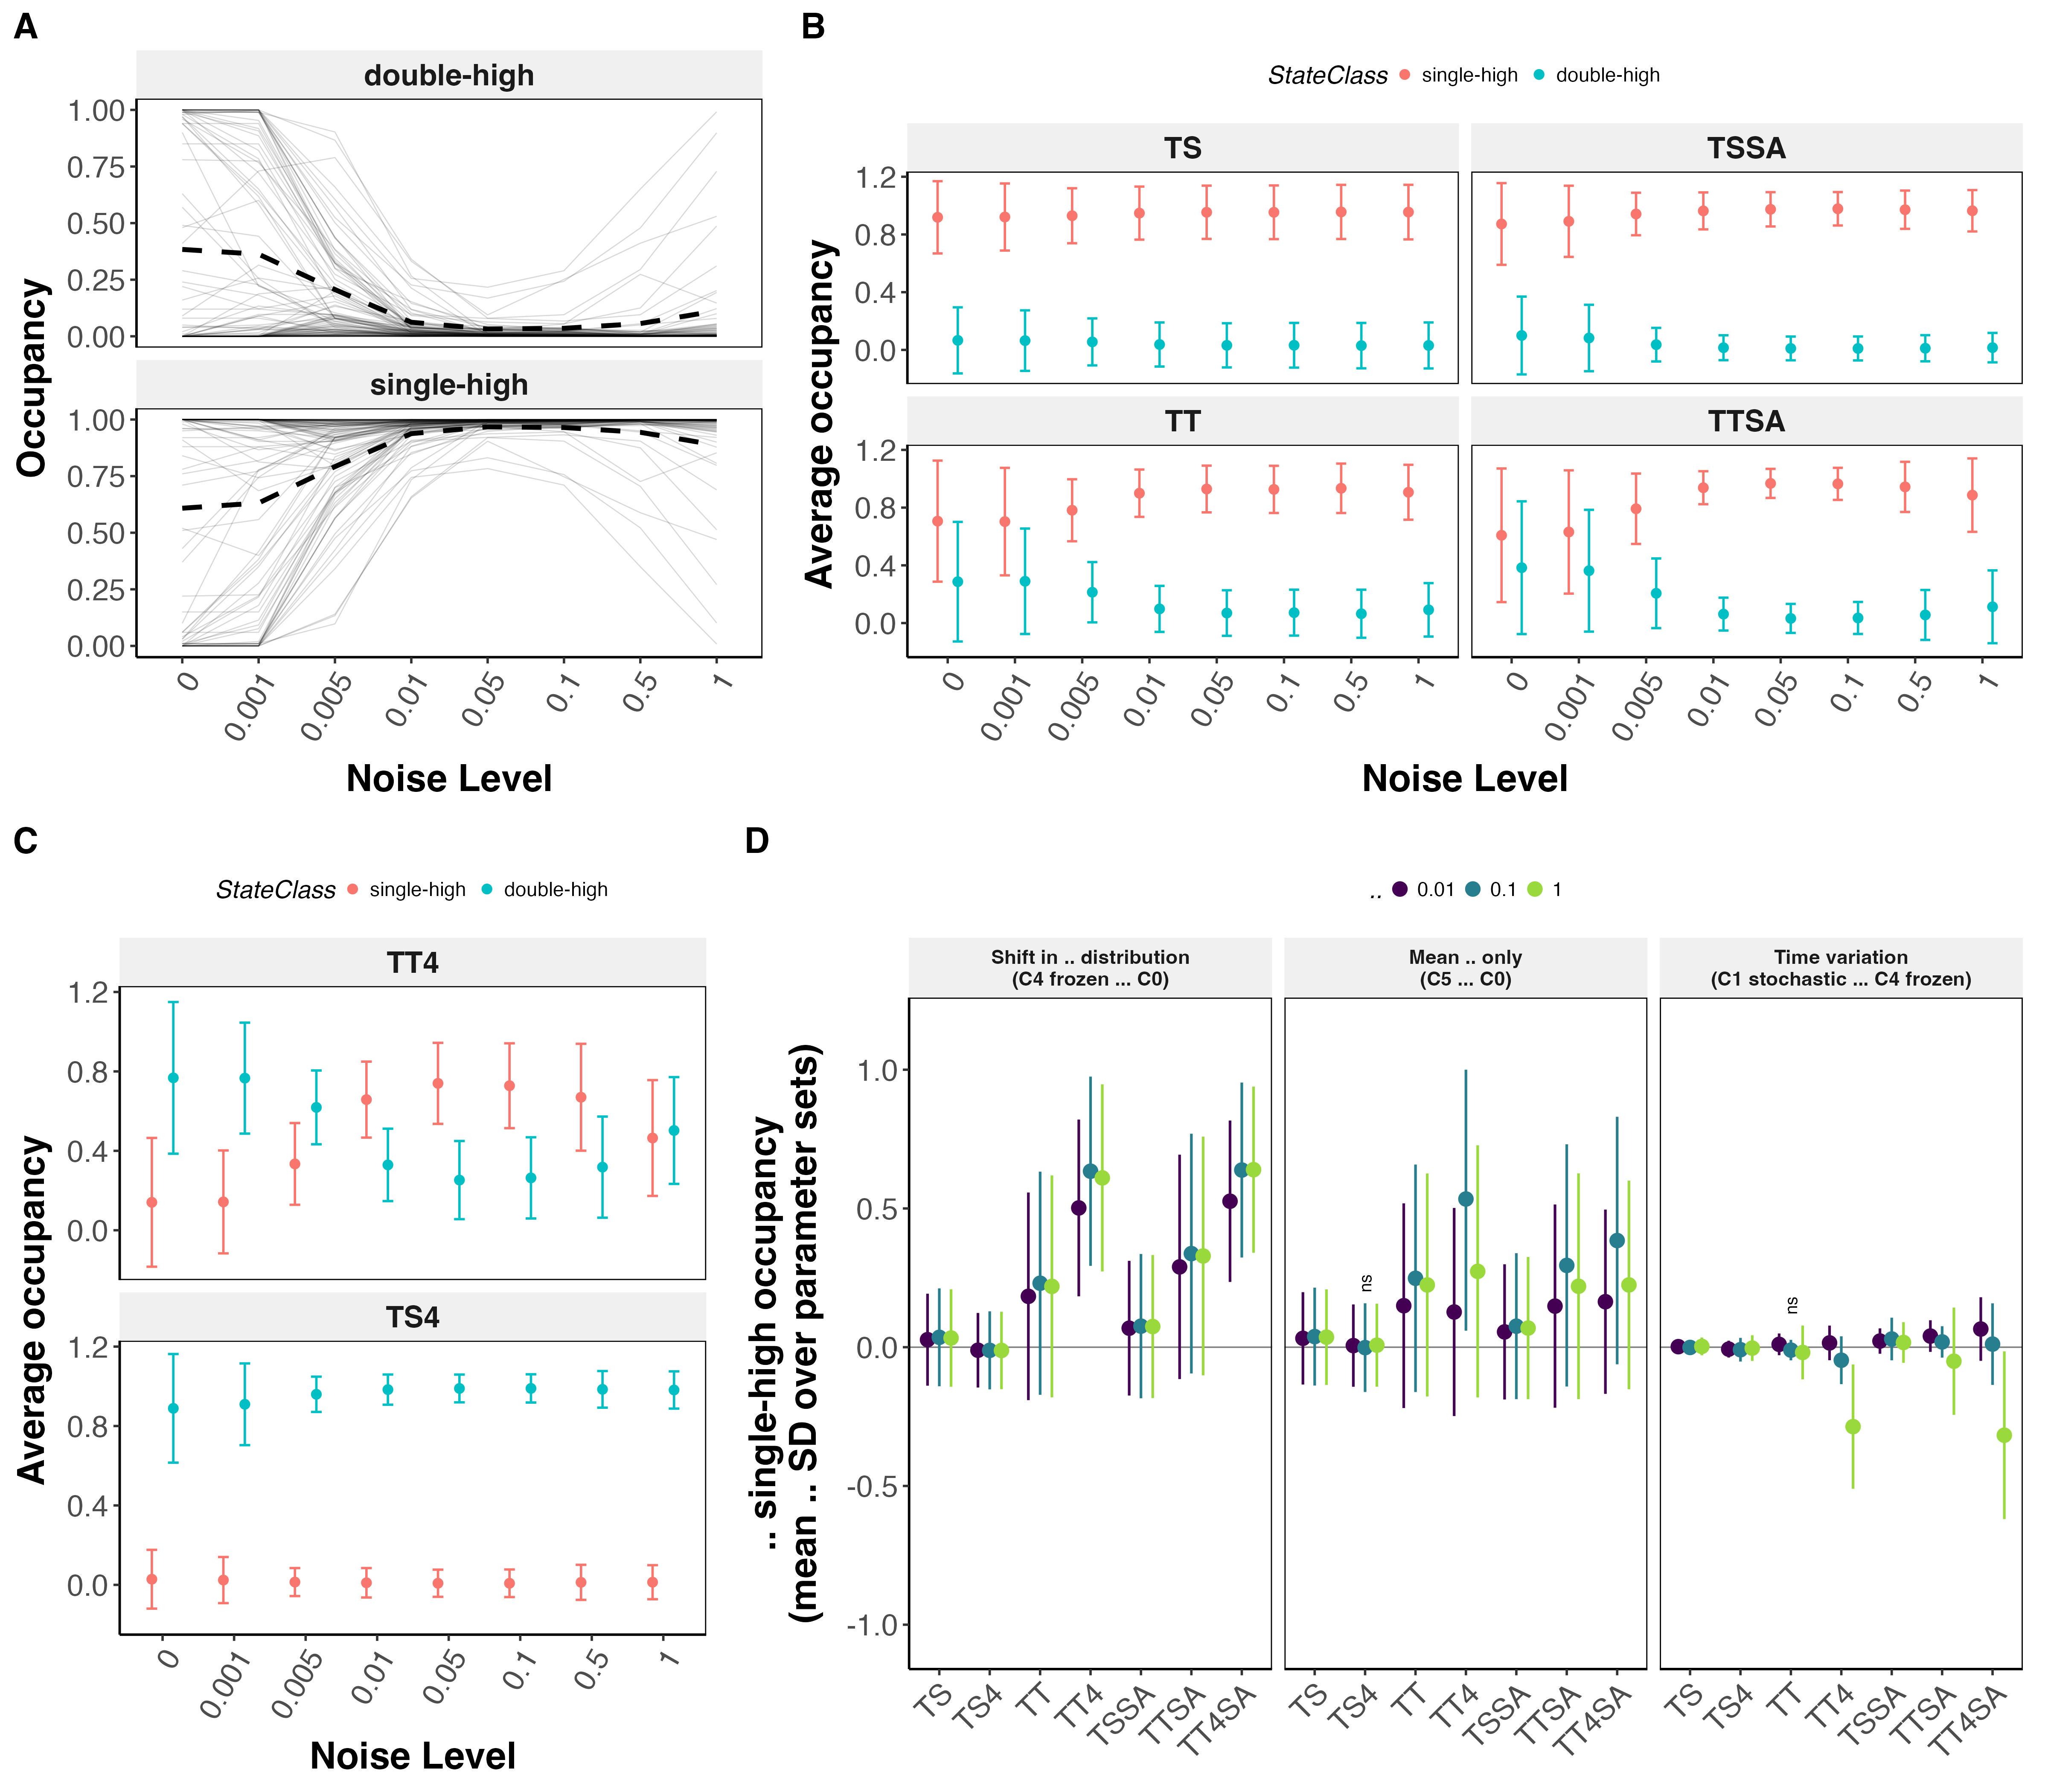
\includegraphics[width=\linewidth]{Fig5.jpg}
    \caption{Effect of multiplicative noise on the phenotypic landscape of cell-fate decision networks.
    \textbf{(A)} Occupancy vs.\ noise level for the TTSA network, single-high and double-high states; grey lines show a random sample of 100 parameter-set trajectories, with the mean across the full parameter population shown separately.
    \textbf{(B)} Average occupancy of single-high vs.\ double-high states vs.\ noise level, for TS, TSSA, TT, and TTSA.
    \textbf{(C)} Same, for the 4-node networks TT4 and TS4.
    \textbf{(D)} Decomposition of the change in single-high occupancy for all seven networks (mean $\pm$ SD over parameter sets of the per-set difference, as in Figure~\ref{fig:3b}E): shift in the $\lambda$ distribution (frozen $\lambda$, C4, $-$ C0), change in mean regulatory strength alone (mean $\lambda$, C5, $-$ C0), and time variation of $\lambda$ (stochastic, C1, $-$ C4), at $\sigma = 0.01$, 0.1 and 1. ns, one-sample Wilcoxon test, Benjamini--Hochberg adjusted $p \geq 0.05$; all other differences have adjusted $p < 0.05$.
    All panels: multiplicative (geometric) rule with maximal regulation $10^{3}$-fold ($\mu_{\min} = 10^{-3}$), $dt = 0.01$; for TS and TSSA the all-high state is counted as double-high.
}
    \label{fig:4}
\end{figure}

% REVISION (R1.3, R3.1): reframed for the geometric rule; numbers from production run 2026-11-csbj-geometric (dt = 0.01 unless stated).
We then analyzed the effect of multiplicative noise in $\lambda$ on the phenotypic landscape. Multiplicative noise multiplies the residual fold-change $\mu$ ($\lambda$ for inhibition, $1/\lambda$ for activation) by a random factor at every update, so each step is proportional to the current value. The walk drifts in $\log\mu$ toward full regulatory strength and settles into a distribution concentrated within about tenfold of the maximal strength, whatever the value of $\sigma$; $\sigma^2/dt$ sets only how quickly it gets there (Methods~\ref{sec:noise}). Multiplicative noise therefore models progressive strengthening of interactions up to a saturation limit, unlike additive noise, where $\lambda$ visits the whole admissible range (Figure~\ref{fig:1}D).

Stronger repression on every edge drives the system toward single-high states (Figure~\ref{fig:4S1}A, i). This changes little in TS, where single-high states dominate to begin with (0.92 without noise, 0.95 at $\sigma = 0.1$; Figure~\ref{fig:1}C). TSSA, which also stabilizes the all-high state without noise, moves toward single-high states as well (0.87 to 0.98; Figure~\ref{fig:4S1}A, ii). The effect is largest in TT and TTSA, which support double-high states nearly as often as single-high states without noise (Figure~\ref{fig:1}C). Under multiplicative noise both converge to single-high states by $\sigma = 0.01$ (TT 0.71 to 0.90, TTSA 0.61 to 0.94; Figure~\ref{fig:4S1}A, iii, \ref{fig:4}A, B). At $\sigma = 1$ the single-high occupancy of TTSA falls slightly (0.89) and its double-high occupancy rises (0.11). This is not a change in the regulatory strengths that are sampled, which give nearly the same frozen-$\lambda$ occupancy at $\sigma = 0.1$ and 1 (0.95 and 0.94), but a consequence of $\lambda$ fluctuating faster than expression can follow (see below).

To further validate this result, we simulated three new networks that are seen in cell-fate decision systems. The first network is an extension of TT network in the context of T cell differentiation, including the regulation of T-reg cells through the transcription factor Foxp3. The resultant four-node network is referred to as toggle tetrahedron (TT4), and is composed of four nodes mutually inhibiting each other. Previous studies have explored this network as well as its self-activation counterpart (TT4SA), our second 4-node network, as candidates for four-fate differentiation~\cite{Duddu2024MultistabilityDifferentiation} (Figure~\ref{fig:4S1}C, i, ii). However, this and other candidate networks for multi-fate systems have so far failed to support the emergence of single-high states representative of fully differentiated cell-fates. TT4 and TT4SA, specifically support only double-high steady states (Figure~\ref{fig:4S1}D). Given the properties of multiplicative noise seen so far, we wanted to study if the double-high states of TT4 and TT4SA could also be driven towards single-high states. The third network is a combination of two mutually inhibiting toggle switches that we refer to as TS4, a representation of coupled cell-fate decision systems often seen in biology~\cite{pasani2020hybrid, hari2022emergent}. TS4 also supports double-high states (Figure~\ref{fig:4S1}D). However, unlike TT4 where all six possible double-high states have equal frequency, TS4 only supports a limited number of double-high states that represent the coexistence of the two binary cell-fate systems. Unlike sequential differentiation, coupled systems are expected to have co-existing phenotypes governed by the network structure. Thus, we asked whether multiplicative noise pushes these coexisting double-high states into single-high states, irrespective of the topology. Under additive noise, all three networks lead to a consistent increase in all-high state, despite the differences in the network structure (Figure~\ref{fig:4S2}A). Under multiplicative noise, TT4 and TT4SA both become dominated by single-high states: single-high occupancy rises from 0.14 to 0.74 in TT4 and from 0.09 to 0.78 in TT4SA at $\sigma = 0.05$ (Figure~\ref{fig:4}C, \ref{fig:4S2}B). At $\sigma \geq 0.5$ it falls again (TT4 0.47, TT4SA 0.42 at $\sigma = 1$), for the same reason as in TTSA. TS4 instead keeps a double-high landscape at every $\sigma$ (double-high occupancy 0.89 without noise, rising to 0.98--0.99 for $\sigma \geq 0.01$), because its double-high states each contain one high node per toggle and are reinforced, not destabilized, when the repression within each toggle strengthens. Thus, unlike additive noise, the effect of multiplicative noise on the phenotypic landscape depends on the network topology.

To separate the effect of the drifted $\lambda$ distribution from that of fluctuations, we compared each stochastic simulation with frozen draws from the $\lambda$ values it visited (C4) and with every edge fixed at its mean $\lambda$ (C5; Methods~\ref{sec:controls}). The frozen draws account for almost all of the change in single-high occupancy, up to $+0.64$ in TT4 and TT4SA, and the mean $\lambda$ alone accounts for less (Figure~\ref{fig:4}D). For $\sigma \leq 0.1$ the stochastic and frozen results agree closely in every network: the largest difference in single-high occupancy is 0.07 (TT4SA at $\sigma = 0.01$, 0.68 stochastic versus 0.62 frozen), and in TT4 at the same $\sigma$ it is 0.02 (0.66 versus 0.64). The enrichment of single-high states is therefore carried by the distribution of regulatory strengths that the noise produces, not by fluctuation as such. At $\sigma \geq 0.5$ the stochastic occupancy falls below the frozen one (TT4 at $\sigma = 1$: 0.47 versus 0.75; TT4SA: 0.42 versus 0.73) and approaches the mean-$\lambda$ control (C5; 0.41 and 0.32). Here $\lambda$ fluctuates faster than expression relaxes, so circuits respond to its time average rather than to its typical value. Under the $\mu^{-2}$ law every decade of the range contributes equally to the mean, which therefore lies several-fold above the median and corresponds to weaker regulation. Consistent with the $\lambda$ process depending on $\sigma$ and $dt$ only through $\sigma^2/dt$, settings with equal $\sigma^2/dt$ give nearly the same occupancy (single-high, $\sigma = 0.01$, $dt = 0.01$ versus $\sigma = 0.1$, $dt = 1$: TT4 0.66 and 0.66, TT4SA 0.68 and 0.69, TT 0.90 and 0.90; Figure~\ref{fig:4S3}). This is unlike additive noise, where the longer update interval changes the outcome at equal $\sigma^2/dt$ (Section~\ref{sec:timescale}).
\begin{figure}
    \centering
    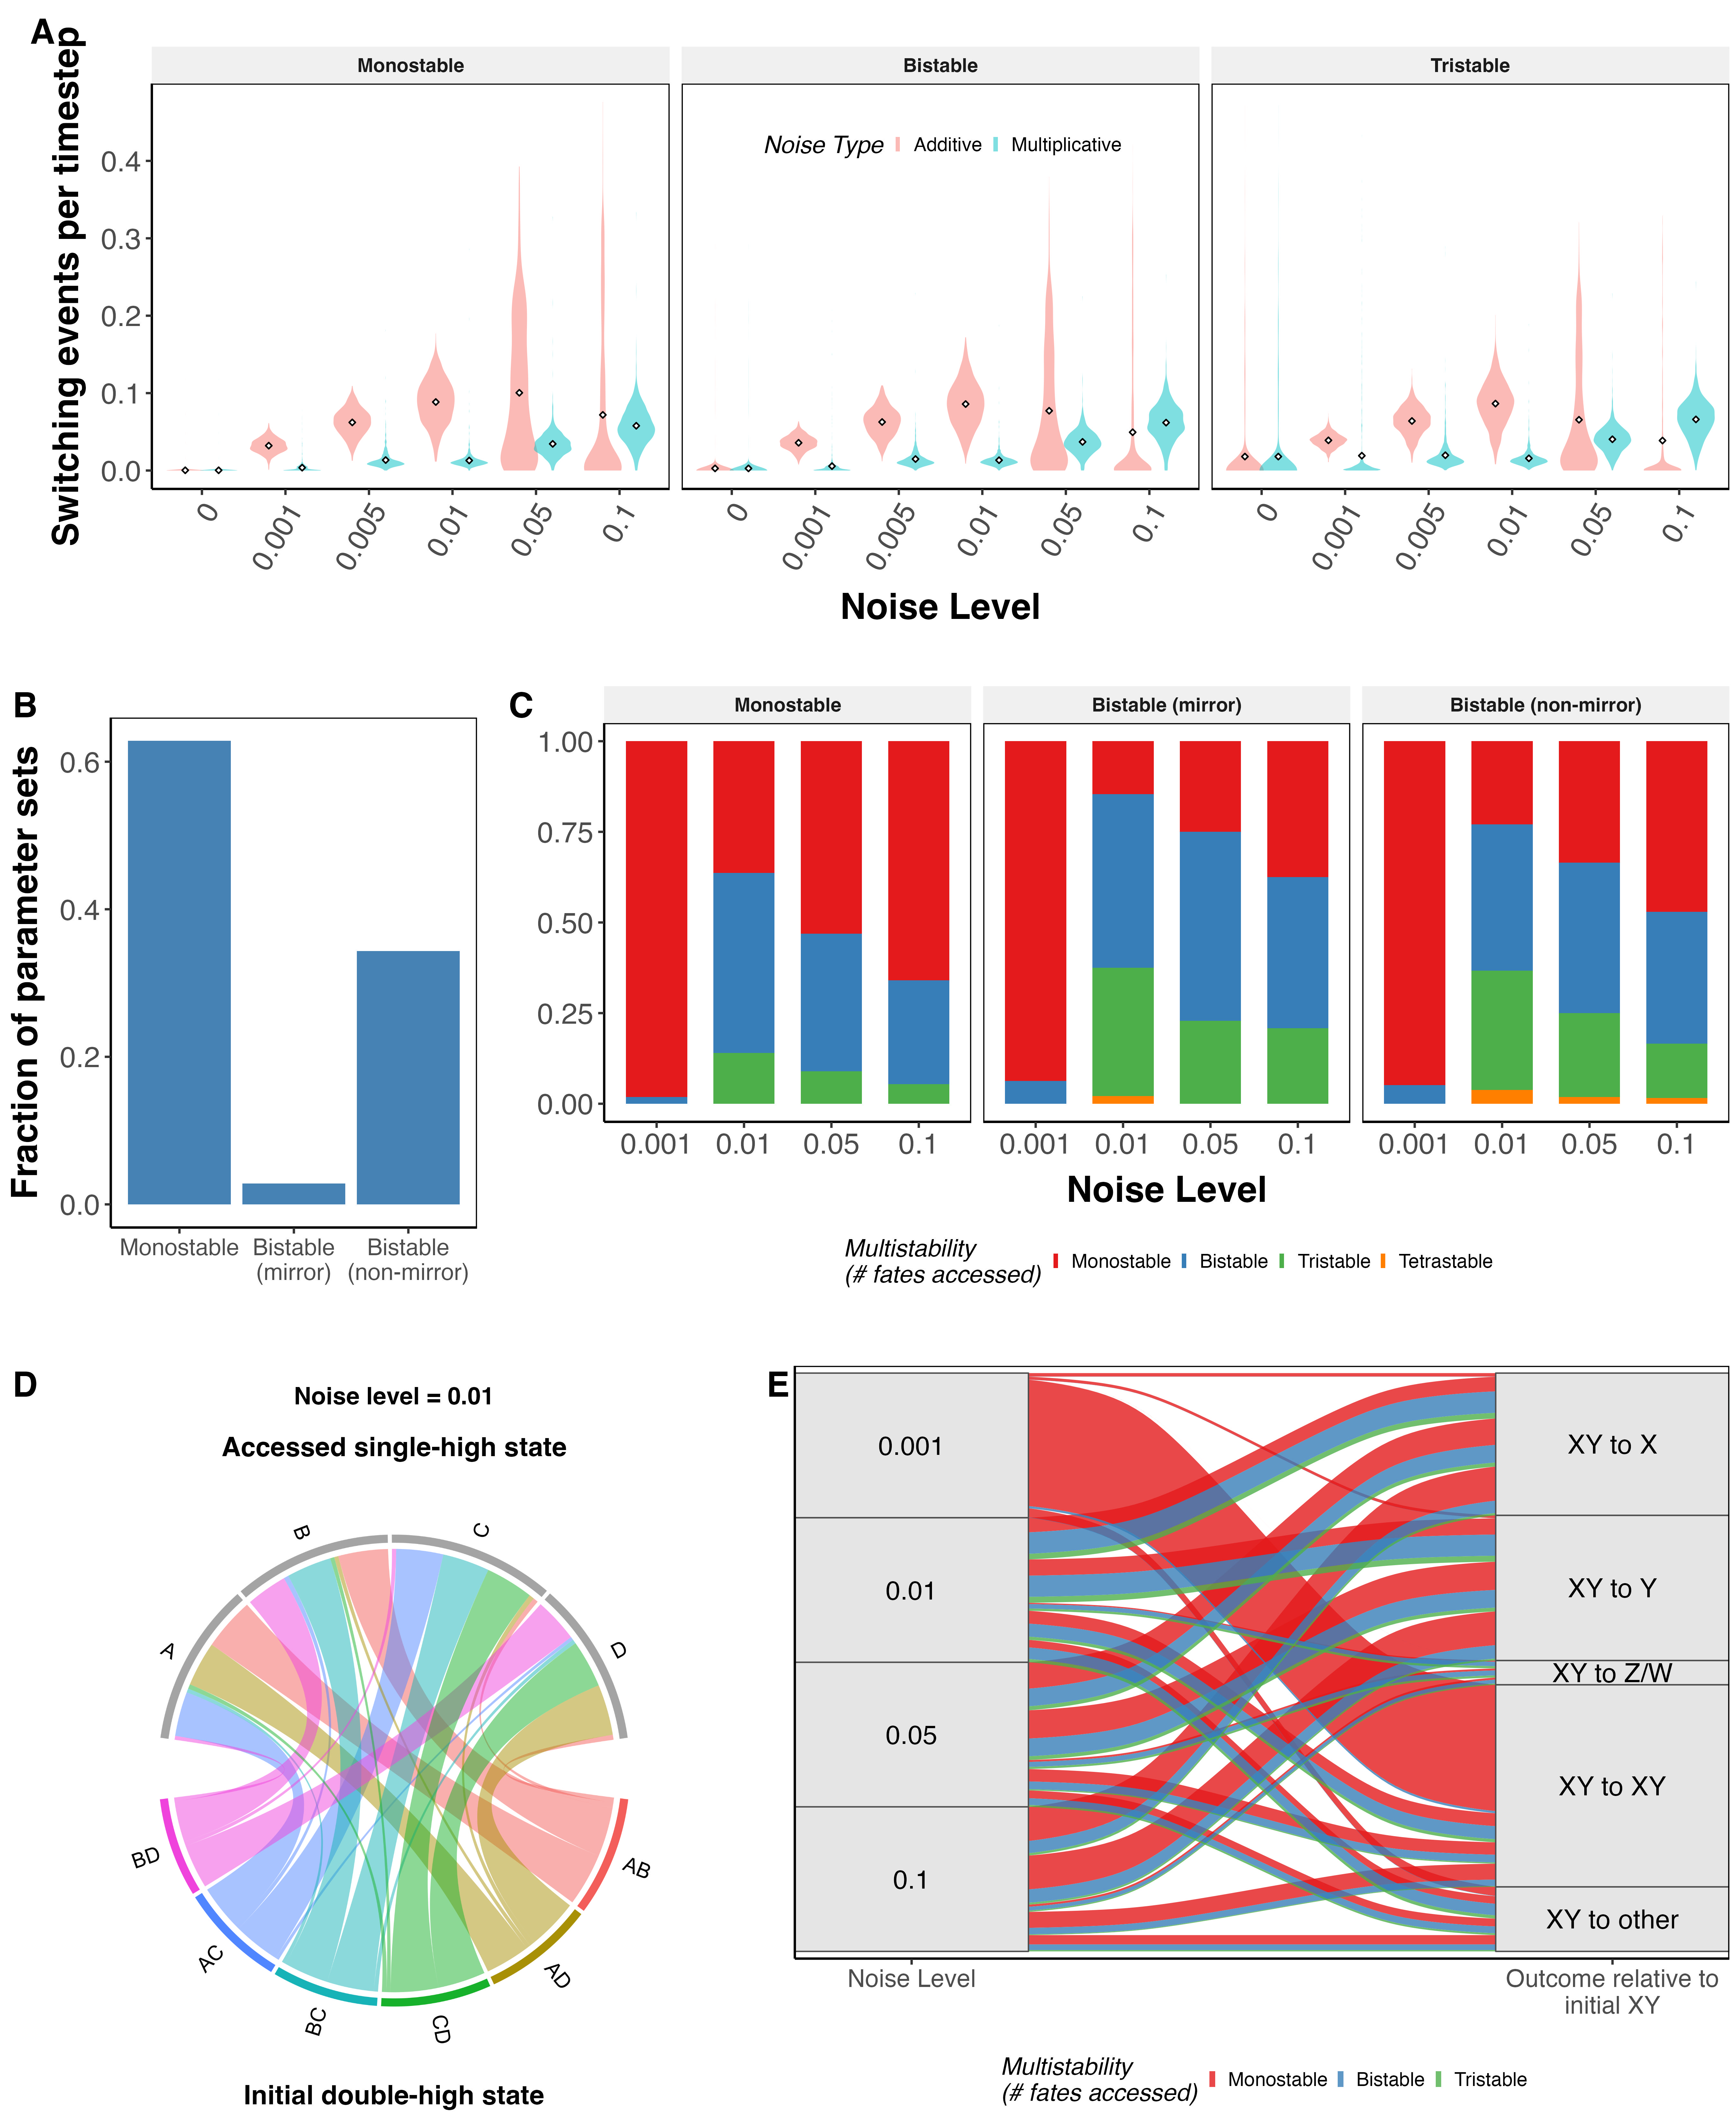
\includegraphics[width=0.9\linewidth]{Fig6.jpg}
    \caption{\textbf{Fate resolution of double-high states in TT4 under multiplicative noise.}
    \textbf{(A)} Switching rate (switching events between discrete states per timestep, after the burn-in window) by noise level, additive versus multiplicative noise, for parameter sets grouped by their number of noise-free steady states; diamonds mark the mean.
    \textbf{(B)} Fraction of the parameter sets with only double-high noise-free steady states in each stability class: monostable, bistable with mirror states (no shared high node), and bistable with non-mirror states (one shared high node).
    \textbf{(C)} For each class in B, fraction of parameter sets accessing 1, 2, 3 or 4 distinct single-high states under multiplicative noise. A state counts as accessed if its occupancy is at least 10\% of that of the most occupied single-high state; for monostable sets the two single-high states not adjacent to the original state are pooled.
    \textbf{(D)} Chord diagram of occupancy from each monostable double-high state (bottom) to the single-high states (top), $\sigma = 0.01$.
    \textbf{(E)} Noise level $\to$ outcome alluvial for the monostable double-high sets, with outcomes relative to the initial double-high state XY (XY to X and XY to Y, adjacent single-high states; XY to Z/W, non-adjacent single-high states; XY to XY, original state; XY to other, any other state), colored by the classification in C. Ribbon widths are normalized within each noise level.
    Multiplicative noise follows the geometric rule ($\mu_{\min} = 10^{-3}$), $dt = 0.01$.
}
    \label{fig:6}
\end{figure}

% REVISION (R1.3, R3.1): production run 2026-11-csbj-geometric.
\paragraph{Origin of the multiplicative effect.} The multiplicative rule has no drift in the mean, but $\log\mu$ drifts by $\approx -\sigma^2/2$ per update (Methods~\ref{sec:noise}), so edges accumulate near maximal regulatory strength. Because this strengthening acts on every edge, including both mutually inhibitory edges of each toggle, the network topology determines that the outcome is enrichment of single-high states. The controls show two regimes (Figures~\ref{fig:4}D, \ref{fig:S_mult_controls}). At low noise ($\sigma = 0.01$), $\lambda$ changes slowly and frozen draws from the visited distribution reproduce the stochastic result (TT4 single-high occupancy: 0.64 frozen versus 0.66 stochastic), whereas the mean-$\lambda$ control does not (0.27). At high noise ($\sigma = 1$), fluctuations are faster than expression relaxation and the stochastic result falls to near the mean-$\lambda$ level (0.47 versus 0.41), well below the frozen control (0.75). The shift toward single-high states is therefore a consequence of the drifted distribution of regulatory strengths, and fast fluctuations counteract it.

% REVISION (R1.3, R3.1): floor sensitivity, pilot 4 (TT4, TT4SA; all 300 sets, 100 per stability class, a subset of the production selection).
\paragraph{Dependence on the maximal regulatory strength.} \label{sec:mult_floor} Because multiplicative noise drives every edge to its full-strength bound, the bound, not $\sigma$, sets the end state (Methods~\ref{sec:noise}). We therefore repeated the TT4 and TT4SA simulations with the inhibitory floor at the RACIPE value of 0.01 and the activation cap at 100. With this floor the mean of the stationary law gives only about 22-fold repression, against about 145-fold at $10^{-3}$, and the single-high enrichment disappears: at $\sigma = 0.1$ ($dt = 0.01$) TT4 single-high occupancy is 0.09, below its noise-free value of 0.12, compared with 0.73 at a floor of $10^{-3}$. TT4SA shows the same contrast (0.06 versus 0.70; noise-free 0.08). The activation cap matters only where activating edges exist: lowering it from 1000 to 100 at a floor of $10^{-3}$ leaves TT4 unchanged (0.73) and reduces TT4SA to 0.59 (Figure~\ref{fig:S_mult_controls}). The enrichment of single-high states under multiplicative noise therefore requires interactions that can strengthen beyond the range sampled by RACIPE, and its size is set by how strong they can become.

\subsection{Multistable double-high states resolve toward their nearest single-high fate across network motifs}

% REVISION (R1.3, R3.1): rewritten for the geometric rule; numbers from production run 2026-11-csbj-geometric (dt = 0.01), CSBJ_review/fig5_6_geometric/fig6_numbers.txt.
We next asked which single-high states the double-high states converge to under multiplicative noise. Is a double-high ``progenitor'' restricted to one terminal fate, or can it access several? We focused this analysis on TT4, which has high double-high and near-zero single-high occupancy without noise (Figure~\ref{fig:4S1}D) and shows the largest shift toward single-high states under multiplicative noise (Figure~\ref{fig:4}C). We first asked whether the states reached under noise are held or only visited transiently, by counting switches between discrete states per timestep after the burn-in window (Figure~\ref{fig:6}A, \ref{fig:6S1}). Under additive noise, the switching rate in TT4 peaked near $\sigma = 0.01$ (mean 0.087 per timestep) and fell at higher $\sigma$ (0.053 at $\sigma = 0.1$), as many parameter sets settled in the all-high state and stopped switching (median 0.003 at $\sigma = 0.1$). Under multiplicative noise, switching was several-fold less frequent at low noise (0.014 at $\sigma = 0.01$) and increased steadily with $\sigma$ (0.037 at $\sigma = 0.05$, 0.062 at $\sigma = 0.1$). This increase is consistent with the timescale effect described above: the larger $\sigma$, the faster $\lambda$ changes relative to expression, and the more often the dominant state changes with it. Across the other networks, multiplicative switching remained near zero in TS and TSSA ($\leq 0.002$ per timestep) and below the additive rate in TT, TTSA and TT4SA for every $\sigma \leq 0.1$ (Figure~\ref{fig:6S1}). The single-high states reached at low-to-moderate multiplicative noise are therefore held, not repeatedly entered and left.

We then classified the TT4 parameter sets whose noise-free steady states are all double-high as monostable, bistable with mirror states that share no high node (e.g.\ AB and CD), or bistable with non-mirror states that share one high node (e.g.\ AB and AD). Monostable sets made up 63\% of these, non-mirror bistable sets 34\% and mirror bistable sets 3\% (Figure~\ref{fig:6}B). Bistable sets, and mirror sets in particular, whose two states together neighbor all four single-high states, might be expected to reach more terminal fates. We therefore counted the single-high states that each parameter set accessed under multiplicative noise (Figure~\ref{fig:6}C). At $\sigma = 0.001$, at least 94\% of the sets in every class accessed at most one single-high state. Access to several fates was greatest at $\sigma = 0.01$, where 64\% of monostable, 77\% of non-mirror and 85\% of mirror bistable sets accessed two or more single-high states, and declined at higher noise (34\%, 53\% and 63\% at $\sigma = 0.1$). Bistable sets thus reached more fates than monostable ones, but none of the classes gave access to all four single-high states in more than 4\% of its parameter sets.

We then characterized the single-high states accessed by monostable double-high parameter sets. For ease of reference, we adopt an alphabetical notation in which a state is denoted by the set of nodes with high expression; for example, $'A'$ represents the single-high state $(1, 0, 0, 0)$ and $'AD'$ the double-high state $(1, 0, 0, 1)$. The single-high states accessed under multiplicative noise were mostly the nearest ones, reached by silencing one of the two active nodes rather than by switching to an unrelated fate: at $\sigma = 0.01$, 92\% of the single-high occupancy of monostable TT4 sets was in one of the two adjacent states (Figure~\ref{fig:6}D; for example, CD sets predominantly access C and D, and rarely A or B). The same held for each double-high attractor separately and in TT, TTSA and TT4SA, where 95--98\% of the single-high occupancy was in an adjacent state (Figure~\ref{fig:6S2}). The outcome depended on the noise level (Figure~\ref{fig:6}E). At $\sigma = 0.001$, most of the occupancy remained in the original double-high state (89\%; XY to XY, where X and Y are any two of the four nodes). For $0.01 \leq \sigma \leq 0.1$, the two adjacent single-high states (XY to X and XY to Y) took 59--68\% of the occupancy, the original state 15--20\%, other states such as different double-high states 11--16\%, and the two non-adjacent single-high states (XY to Z/W) only 5--6\%. The non-adjacent share did not grow at higher noise (2\% at $\sigma = 1$). This picture is consistent with multiplicative noise strengthening inhibition. The relative strengths of the inhibitions determine which double-high state is stable, with the inhibitions on the low-expression nodes stronger than those on the high-expression nodes~\cite{Duddu2024MultistabilityDifferentiation}. When every edge is strengthened toward its maximum, one of the two high nodes comes to repress the other, and which one is silenced depends on which of the inhibitions incoming to the two high nodes was already stronger. Reaching a non-adjacent single-high state would instead require a low node to be released from its inhibitions, which the drift toward full strength opposes, so such transitions remain rare at every noise level. We found the same nearest-fate commitment in TT, TTSA and TT4SA (Figures~\ref{fig:6S2}, \ref{fig:6S3}), indicating that the ability of multiplicative noise to push hybrid, progenitor-like states toward terminally differentiated ones follows their nearest available fate in all of these topologies rather than being specific to TT4.

We extended the noise-level $\to$ fate alluvial analysis of Figure~\ref{fig:6}E to the bistable double-high classes (Figure~\ref{fig:6S3}). Mirror bistability is structurally impossible in the 3-node TT and TTSA networks (any two double-high states of three nodes share an active node), so only their non-mirror class is shown (Figure~\ref{fig:6S3}A, B); TT4 has enough parameter sets in both classes to show them separately (Figure~\ref{fig:6S3}C), while TT4SA's mirror bistable population (14 parameter sets) is too sparse to interpret alone and is pooled with its non-mirror population (Figure~\ref{fig:6S3}D). At $\sigma = 0.1$, the original double-high states of bistable sets retained a share of the occupancy similar to that of monostable sets (TT4: 0.20 mirror and 0.22 non-mirror versus 0.16 monostable; TT 0.14 versus 0.12; TTSA 0.10 versus 0.08; TT4SA 0.23 versus 0.25). We base the quantitative statements above on the monostable class, where each parameter set has a single reference state.

\subsection{Effects of regulatory noise on the phenotypic landscape scale to larger biological networks}

While the toggle switch and TSSA are well-studied representatives of binary cell-fate decision systems, the regulatory circuits underlying real cell-fate transitions are rarely small or as isolated. Phenotypes emerge from coordinated expression across tens to hundreds of genes, many of which function as transcription factors that individually regulate transitions between phenotypes. It is therefore important to ask whether the noise-driven dynamics observed in small motifs generalize to larger, more complex GRNs. To address this, we asked whether biological GRNs governing two well-studied cell-fate decisions -- epithelial-mesenchymal plasticity~\cite{hari2022landscape} and Gonadal cell-fate decision~\cite{rios2015boolean} -- behave similarly to our studied examples.

Large-scale GRNs underlying binary cell-fate decisions often share a common coarse-grained structure: nodes can be partitioned into two ``teams'', with intra-team interactions predominantly activating and inter-team interactions predominantly inhibitory (Figure~\ref{fig:7S1}). At a coarse-grained level, this structure is analogous to a TSSA, with each super-node representing the collective of genes defining one phenotype. The biological GRNs adhere to this structure at a coarse-grained level as well. One specific EMT model, a 23-node network underlying the epithelial-mesenchymal transition (EMT)~\cite{Huang2017}, has two teams of nodes corresponding to the epithelial and mesenchymal phenotypes respectively. In fact, we previously showed that many large-scale EMT GRNs constructed to date could be coarse-grained into two mutually inhibiting teams, and that the presence of these teams gives rise to a robust, low-dimensional phenotypic landscape despite the size of these networks~\cite{hari2022landscape,tripathi2023minimal,hari2023low}. We also showed that these teamed networks are robust to noise in the network state, and extensive mutations disrupting the network of positive feedback present in these GRNs are required to stabilize what is otherwise a weakly stable hybrid phenotype~\cite{rashid2022network, Hari2025APlasticity}. The 19-node gonadal network, governing cell-fate decisions between Sertoli and Granulosa fates that are upstream of male and female development respectively~\cite{rios2015boolean}, has two teams of nodes corresponding to Sertoli and Granulosa phenotypes, and carries the advantages of team structure across simulation formalisms~\cite{Hari2025LowNetworks, Shyam2025MutuallyNetworks}.

Given the size of these networks, exploration of regulatory noise using similar ODE based models as with small-scale networks earlier would be computationally infeasible. Hence, we utilized a threshold-based Boolean formulation to analyze these networks instead \cite{FontClos2018}. In this formalism, each node is allowed to take either -1 (low) or +1 (high) expression levels. The edges of the network are given a weight of +1 (activation) or -1 (inhibition). The state of the network is updated asynchronously, based on an Ising-model-inspired, additive rule (see Methods). Regulatory noise perturbs the magnitudes of the edge weights while keeping their signs. In the standard threshold rule, weakening an edge only shifts the balance among the remaining inputs of its target, whereas in the RACIPE models weakening an interaction moves its target toward maximal production regardless of the regulator. We therefore used the Boolean limit of the RACIPE production term, in which each node keeps a fixed activation threshold, so that weakening any incoming edge biases the target toward the active state (Eq.~\ref{eq:boolbias}, Methods). The rule is identical to the standard one for the unperturbed weights. The binary state vectors ($S \in \{0, 1\}^N$) were converted into team scores --- the fraction of nodes in each team that are active --- and a phenotypic score defined as the difference between the two team scores. Values near $\pm 1$ indicate terminal phenotypes (epithelial/mesenchymal or Sertoli/Granulosa), while values near 0 indicate hybrid states. Under deterministic conditions, the phenotypic landscape is largely concentrated in regions corresponding to terminal states with team scores $\pm$ 1. 

\begin{figure}
    \centering
    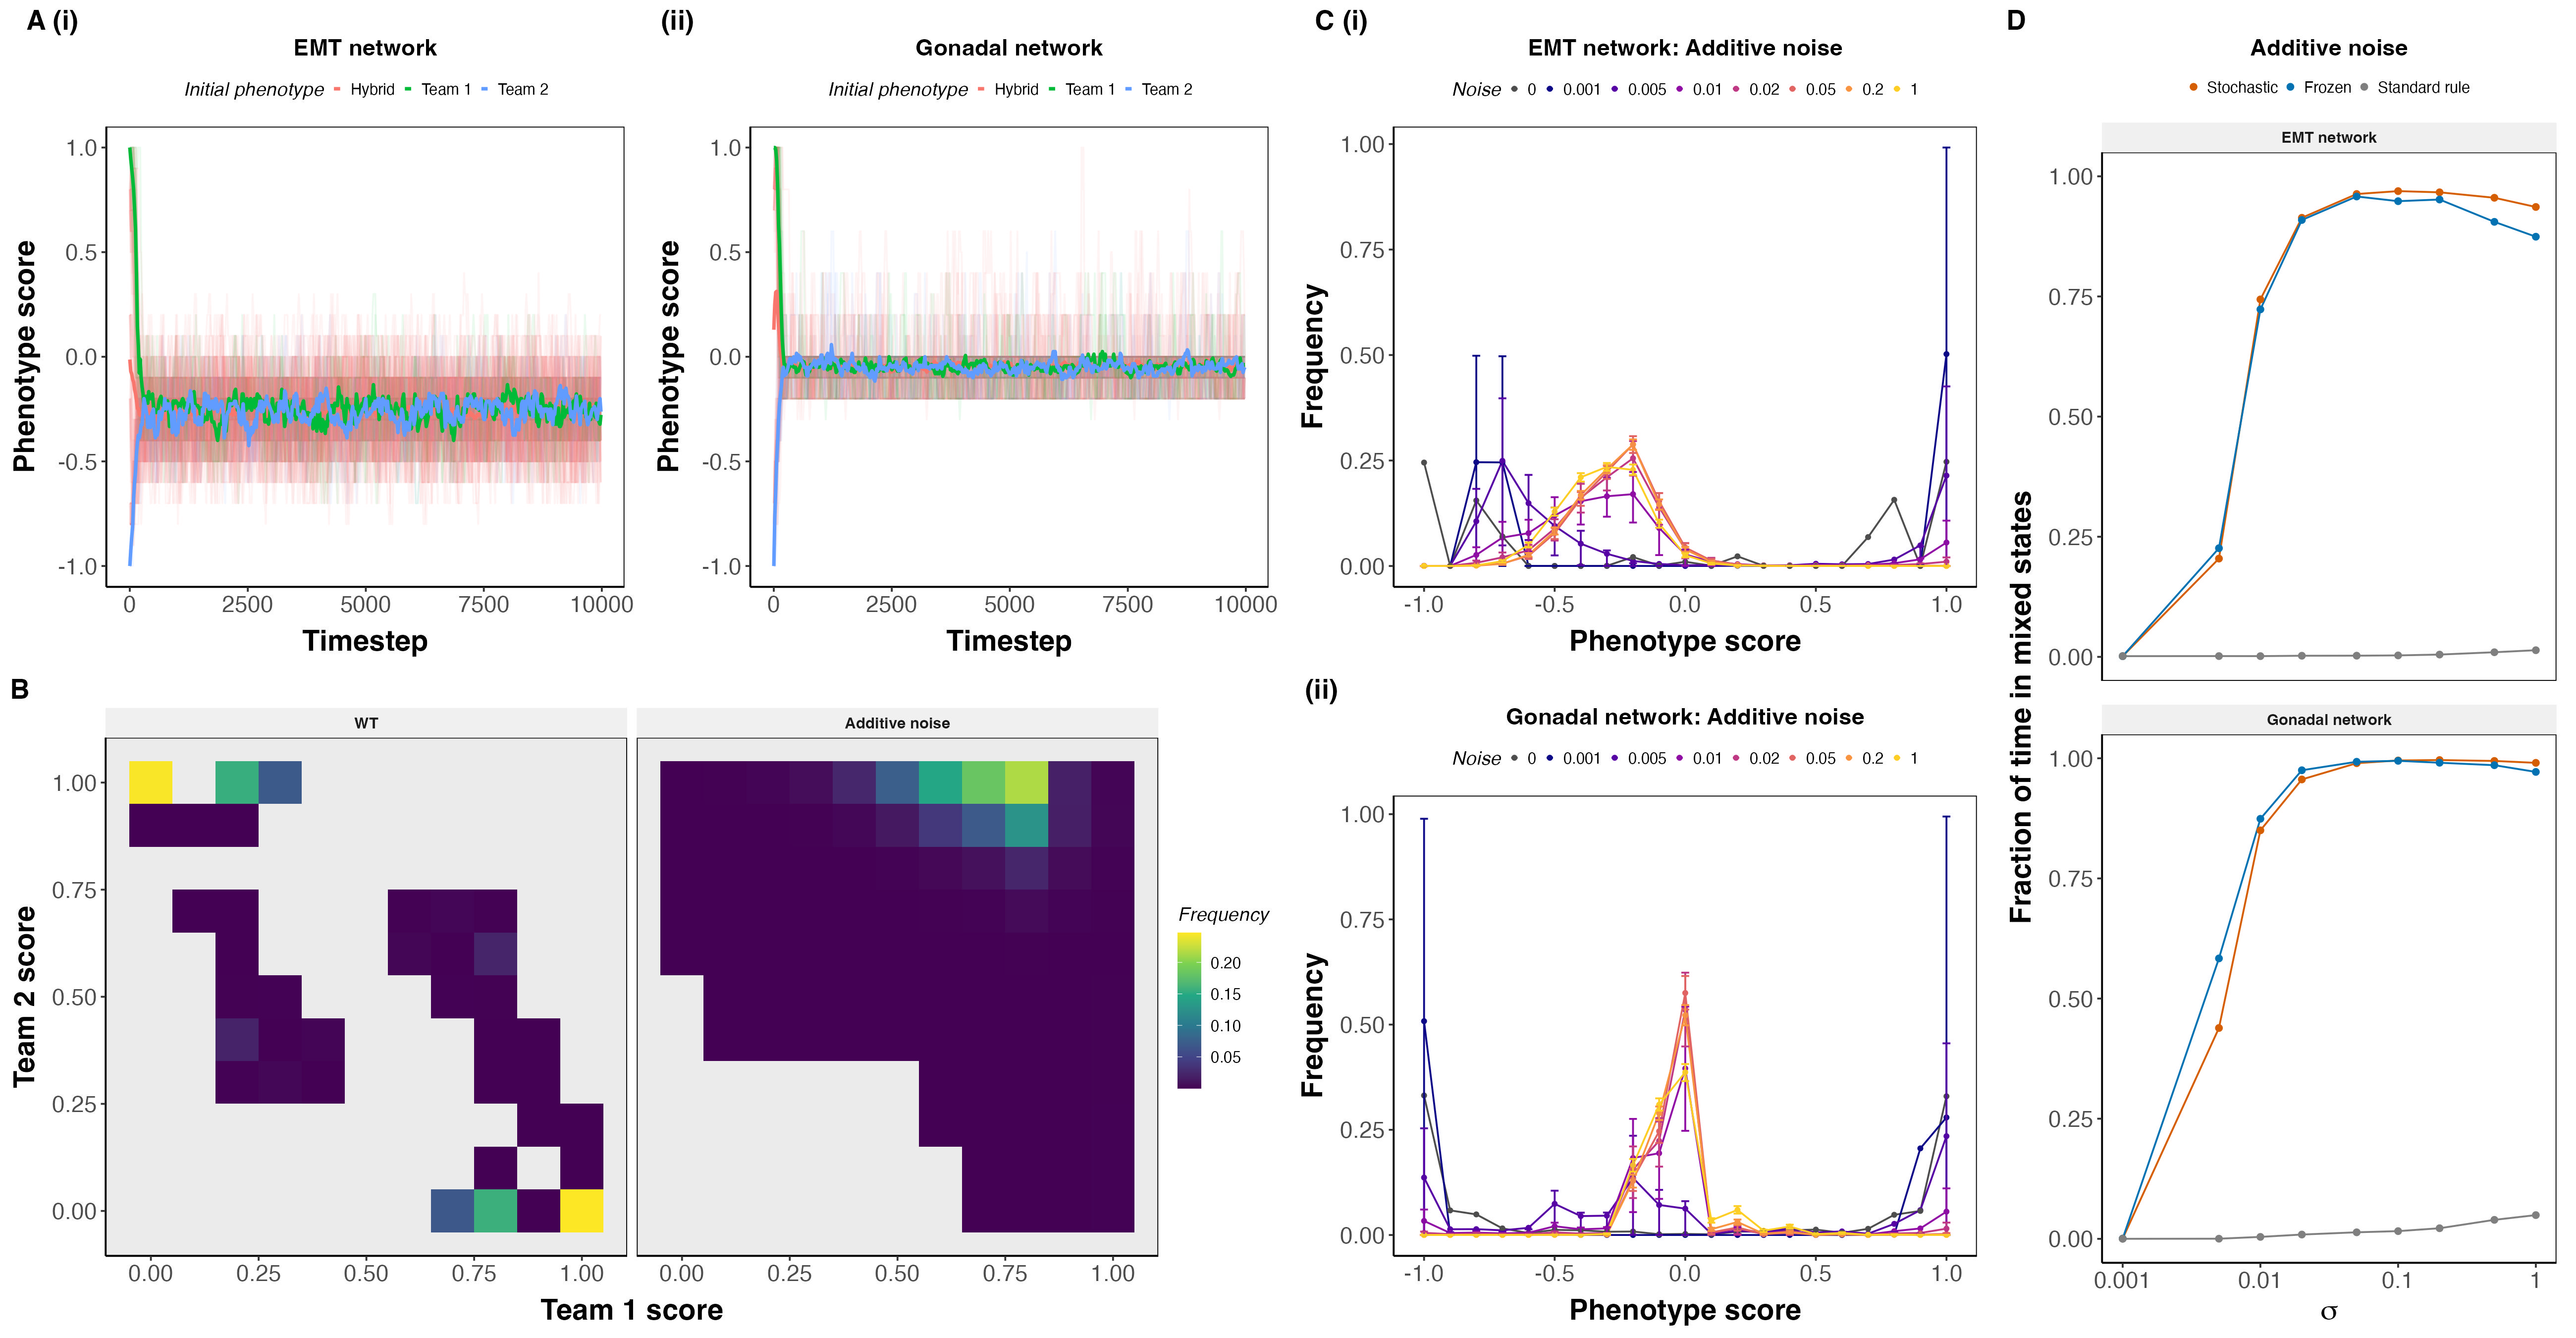
\includegraphics[width=\linewidth]{Fig7.jpg}
    \caption{\textbf{Regulatory noise in large-network Boolean models.} All perturbed simulations use the ODE-equivalent threshold rule (Eq.~\ref{eq:boolbias}). A) Phenotypic-score trajectories (100 of 1000) for the EMT (i) and gonadal (ii) networks under additive noise, $\sigma = 0.05$, coloured by the phenotype of the initial state; thick lines, mean. B) Team-score density for the EMT network: steady states of the unperturbed network (WT) and the trajectories in A (additive noise), from low (blue) to high (yellow) frequency. C) Fraction of time spent at each phenotypic score under additive noise, mean and interquartile range over 1000 trajectories, for (i) EMT and (ii) gonadal networks; $\sigma = 0$ is the steady-state distribution of the unperturbed network. D) Fraction of time in mixed states ($|\text{phenotypic score}| \le 0.5$) against $\sigma$ under additive noise, for stochastic weights, frozen weights drawn from the same time-pooled distribution, and the standard threshold rule without the ODE-equivalent threshold. Stationary noise is shown in Figure~\ref{fig:7S2}.}
    \label{fig:7}
\end{figure}

Under additive noise, both biological networks show behavior consistent with the small network analysis. Trajectories initiated from terminal and hybrid steady states of the unperturbed network converge on hybrid phenotypic scores within a few hundred time steps and remain there (Figure~\ref{fig:7}A, B; Figure~\ref{fig:7S2}A). The fraction of time in mixed states ($|\text{score}| \le 0.5$) rises from below 0.01 at $\sigma = 0.001$ to 0.74 (EMT) and 0.85 (gonadal) at $\sigma = 0.01$, and to 0.96 and 0.99 at $\sigma = 0.05$, changing little at higher noise (Figure~\ref{fig:7}C, D). At $\sigma = 0.001$ the weights move too little within $10^4$ steps to reach this regime. Stationary noise leaves the landscape close to that of the unperturbed network for $\sigma \le 0.2$ (mixed fraction $\le 0.04$), and produces mixed states only at $\sigma \ge 0.5$ (0.51 and 0.82 at $\sigma = 1$), where clamping at the maximal magnitude lowers the mean edge weight (Figure~\ref{fig:7S2}B, C).

As in the ODE models, the shift arises mainly from the change in the distribution of edge weights. Trajectories with frozen weights drawn from the same time-pooled distribution reach nearly the same mixed fraction as the stochastic ones (within 0.03 for $0.01 \le \sigma \le 0.2$), and time variation adds a small further gain only at the highest noise ($\sigma = 1$: 0.94 vs 0.87 in EMT; both-team activation 0.92 vs 0.82 in gonadal) (Figure~\ref{fig:7}D). The effect requires the ODE-equivalent threshold: with the standard rule, in which weakening an edge does not bias its target toward activation, additive noise only modestly lowers terminal-state occupancy and mixed states stay below 0.05 at all noise levels (Figure~\ref{fig:7}D). The hybrid states are thus reached through the same regulator-independent derepression that enriches all-high states in the small motifs.

The two networks differ, however, in the characteristics of their hybrid states. In the EMT network, the mesenchymal team becomes fully active while most of the epithelial team is also active, so that the phenotypic score settles near $-0.2$ to $-0.3$ rather than at zero (Figure~\ref{fig:7}B, C(i)); both teams are at least 80\% active for only 0.18 of the time at $\sigma = 0.05$. In the gonadal network, both teams become almost fully active (0.96 of the time at $\sigma = 0.05$) and the score collapses to near zero (Figure~\ref{fig:7}C(ii)). % REVISION: asymmetry explained from in-edge signs (Boolean/ContWeightPert/WT_signfix/*.topo, *.teams).
The difference follows from the signs of the inputs to each node. When both teams are active, a node whose inhibitory inputs outnumber its activating ones receives a net negative input, and the bias in Eq.~\ref{eq:boolbias} offsets it only after substantial weakening of its incoming edges. In the EMT network, 9 of the 12 epithelial nodes are of this kind, most of them microRNAs that receive only inhibitions from mesenchymal transcription factors, compared with 4 of the 11 mesenchymal nodes. These epithelial nodes keep switching off while the mesenchymal team stays active, which shifts the hybrid score below zero. In the gonadal network, only 2 of 13 Sertoli and 1 of 5 granulosa nodes have more inhibitory than activating inputs, so both teams can remain active together. The position of the hybrid state therefore depends on how inhibition is distributed across the nodes of each team, not only on the team structure. Overall, our results indicate that regulatory noise can have a significant impact on the phenotypic landscape, with the direction of the impact determined by the nature and the magnitude of the noise. While additive noise can drive the cell-fate decision system up towards an undifferentiated phenotype, multiplicative noise can drive the system down towards a terminally differentiated state (in the ODE models). 
% \begin{figure}
%     \centering
%     \includegraphics[width=\linewidth]{Schematic.png}
%     \caption{\textbf{Schematic representation of regulatory-noise-induced remodeling of the phenotypic landscape.} The landscapes reimagine Waddington’s phenotypic landscape \cite{waddington1953} in the context of the toggle triad. In the deterministic (WT) system (center), hybrid (double-high) and terminally differentiated (single-high) states constitute stable attractors. Additive noise (left) reshapes the landscape by stabilizing an undifferentiated all-high state, whereas multiplicative noise (right) drives the transitions from hybrid states to terminally differentiated states. Colored sectors indicate the nodes expressed in each state.}
%     \label{fig:schematic}
% \end{figure}

\section{Discussion}

Historically, regulatory interactions in gene networks models have been remarkably successful at predicting cell-fate outcomes from EMT circuits to Boolean perturbation frameworks. Nonetheless, stochasticity in kinetic parameters is unavoidable. Therefore, here, we introduced regulatory noise into GRN models by allowing the fold-change parameter governing regulatory efficacy of a TF to be a stochastic process. We found that regulatory noise can significantly alter the phenotypic landscape, with qualitatively different outcomes depending upon the \emph{mode} of regulatory noise. Across cell-fate decision motifs, additive noise drove networks toward hybrid co-expression states, multiplicative noise favored single-high terminal states, and stationary noise largely preserved the deterministic landscape at low-to-moderate noise. These effects were reproduced qualitatively in two well-characterized biological GRNs, namely EMT and gonadal cell-fate determination, suggesting that regulatory stochasticity can act not merely as a perturbation around a fixed landscape, but as a determinant of which regions of that landscape are occupied.

% \paragraph{Regulatory noise can cloud the inference of network topology.}
Prior theoretical work has shown that noise can alter the effective bistable range of regulatory circuits and generate switch-like population distributions even in deterministically monostable systems~\cite{OchabMarcinek2010w}. Our results extend this idea to stochasticity in the regulatory interactions themselves. The $(1, 1)$ co-expression state, negligible in the deterministic toggle-switch landscape, becomes dominant under additive noise, whereas multiplicative noise can generate single-high states in networks such as the toggle tetrahedron where these states are not stable deterministically. Thus, similar population-level expression patterns can arise from different combinations of network topology and regulatory-noise regime. A positive correlation between two genes, for example, need not imply mutual activation if stochasticity of mutual inhibition can generate the same pattern. Inferring regulatory wiring from steady-state expression data without accounting for regulatory stochasticity may therefore attribute noise-induced phenotypes to structural features that are not actually present.

% \paragraph{Regulatory noise exposes a hierarchy of molecular timescales.}
The three noise modes studied here can be viewed most usefully not as literal descriptions of individual molecular mechanisms, but as phenomenological limits of how fluctuations in regulatory efficacy evolve in time. This distinction is particularly relevant for intrinsically disordered TFs, for which regulatory function emerges from conformational ensembles spanning a hierarchy of timescales. Rapid conformational fluctuations may be effectively averaged over by the slower transcriptional response, whereas post-translational modifications can stabilize particular conformers for minutes to hours~\cite{Kulkarni2022, Kulkarni2019}. Still slower processes, including chromatin remodeling and epigenetic feedback, can provide cellular memory across timescales much longer than that of an individual binding event.

Stationary noise represents the regime closest to the conventional deterministic approximation: regulatory parameters fluctuate around a preferred set of values and therefore retain memory of their underlying interaction strength. At low-to-moderate noise, such fluctuations have little effect on phenotype occupancy, consistent with a separation of timescales in which sufficiently rapid or sufficiently constrained molecular fluctuations are averaged into an effective deterministic parameter. Only at high noise does boundary sampling appreciably reshape the landscape.

Additive noise represents the opposite limit. Here, $\lambda$ undergoes a bounded random walk whose long-term distribution loses memory of its initial value. For inhibitory interactions, this progressively increases access to weakly repressive configurations and drives the system toward hybrid co-expression states. A possible molecular analogue is unconstrained sampling of an IDP conformational ensemble or regulatory configurations generated by non-specific binding, in which successive changes in effective regulatory strength are only weakly anchored to the previous interaction state~\cite{Ferrie2022Structure-functionRegulation, Holehouse2023TheRegions}. Importantly, our $\Delta t$ analysis shows that the resulting phenotype shift depends on the relative timescales of parameter fluctuation and expression relaxation. When $\lambda$ changes rapidly enough that expression cannot fully relax to the instantaneous landscape, additive noise produces an additional hybrid-state enrichment beyond that predicted by the stationary $\lambda$ distribution alone. Thus, the ratio between the correlation time of regulatory fluctuations and the response time of the downstream GRN may itself be an important determinant of cellular plasticity.

Multiplicative noise produces a qualitatively different outcome because the magnitude of each perturbation depends on the current value of $\lambda$. This creates a self-reinforcing drift toward stronger regulation that ends at a saturation limit, the maximal strength an interaction can reach, and consequently drives the circuits toward single-high states. The size of the effect is set by that limit, and the noise amplitude sets only how fast it is reached. Processes that progressively stabilize a binding mode up to a maximal strength provide possible conceptual analogues: induced-fit binding, PTM-dependent stabilization of particular conformational substates, which persist much longer than rapid conformational exchange and can switch binding~\cite{Kulkarni2022, Kulkarni2019, Bah2015Folding}, and epigenetic locking~\cite{Jia2019}. We do not interpret multiplicative noise as a direct model of any specific modification process; rather, it captures the qualitative consequences of introducing state-dependent memory into the evolution of regulatory strength. Its effect is carried by the drifted distribution of regulatory strengths rather than by fluctuation as such: frozen draws from that distribution reproduce it, and very fast fluctuations weaken it, because the circuit then responds to the average regulatory strength.

% REVISION (R1.4, R3.5): what the controls show for both noise modes.
The controls separate two ways in which regulatory noise acts. First, it changes the distribution of regulatory strengths that a circuit experiences, and frozen draws from this distribution account for most of the effect of additive noise at low amplitude and of multiplicative noise at all but the highest amplitude. Second, its timescale relative to gene expression determines what fluctuation adds. When $\lambda$ changes faster than expression relaxes, circuits respond to the time-averaged regulation: under additive noise this further enriches all-high states, because derepression acts whatever the state of the regulator, whereas under multiplicative noise it weakens the single-high shift, because the average lies further from maximal strength than the typical value. Regulatory noise is therefore characterized by at least three quantities: its magnitude, its dependence on the current regulatory state, and its timescale relative to gene-expression dynamics.

% \paragraph{The effect generalizes to biological cell-fate networks.}
The additive-noise phenotype generalized from small motifs to the 23-node EMT and 19-node gonadal cell-fate networks once the Boolean model was given the property that drives it in the ODE models: weakening an interaction moves its target toward activation regardless of the regulator. With this threshold rule, additive noise replaced terminal states with hybrid states in both networks, whereas stationary noise caused little change except at the highest amplitudes. As in the motifs, frozen weights from the same distribution reproduced most of the effect. Without this rule, weight noise only modestly reduced terminal-state occupancy, which shows that the effect depends on how weakened regulation is represented rather than on weight heterogeneity alone. The specific hybrid states nevertheless differed: the EMT network kept its mesenchymal team fully active with partial epithelial activation, whereas the gonadal network approached full activation of both teams. Thus, the tendency of additive noise to increase phenotypic mixing appears robust across network scales and formalisms, while the particular hybrid configurations accessed remain constrained by network structure.

This result is especially relevant to epithelial--mesenchymal plasticity. Hybrid epithelial/mesenchymal (E/M) states are associated with stemness, collective migration, metastatic competence, and therapy resistance~\cite{Pastushenko2019EMTMetastasis, jolly2015implications, pasani2020hybrid, Sahoo2021}. Our results identify fluctuations in regulatory efficacy as one possible route to their enrichment: additive-like noise is sufficient to shift both an isolated bistable motif and a full EMT network toward hybrid phenotypes without changing network topology. Mutations affecting intrinsically disordered regions may therefore alter phenotype distributions not only through conventional gain- or loss-of-function effects, but also by changing the magnitude, persistence, or correlation structure of fluctuations in regulatory activity~\cite{Kulkarni2023IntrinsicallyLater}.

% \paragraph{Chromatin state may control the transition from exploration to locking.}
The connection between regulatory noise and phenotype is likely to extend beyond TF conformational dynamics to the chromatin environment in which regulatory interactions occur. Pluripotent and progenitor cells maintain relatively open, dynamic chromatin and broadly accessible transcriptional programs~\cite{Meshorer2006HyperdynamicCells, Efroni2008GlobalCells}. Recent work further suggests that fluctuations in chromatin accessibility can actively enable ectopic or multi-lineage-like transcriptional programs~\cite{Gamble2025}. Such a permissive chromatin state increases the number of genomic configurations accessible to TFs and may therefore enhance fluctuations in effective regulatory strength. At a coarse-grained level, this resembles the additive-noise regime: regulatory interactions explore a broader range of efficacies, weakening the confinement imposed by the deterministic network and increasing access to hybrid states.

Differentiation, however, is accompanied not simply by reduced transcriptional heterogeneity but by progressive stabilization of regulatory programs through chromatin remodeling and epigenetic feedback. This introduces a much slower form of memory than IDP conformational fluctuations. A useful example comes from EMT, where epigenetic feedback has been shown theoretically and experimentally to make phenotype transitions increasingly difficult to reverse. In earlier work on the miR-200/ZEB EMT circuit, prolonged TGF-$\beta$ exposure progressively reduced the ability of cells to revert toward the epithelial state following withdrawal of the inducing signal, consistent with epigenetic feedback stabilizing the mesenchymal program \cite{Jia2019, Jia2020EpigeneticEMT}. Such ``locking'' changes the problem from one of fluctuations around a regulatory state to one in which the history of the system progressively reshapes its future transition probabilities.

We propose, as a hypothesis for future work, a hierarchy of regulatory dynamics. Fast conformational fluctuations could perturb interaction strengths on timescales shorter than gene-expression relaxation; modifications that stabilize particular conformations or binding modes could strengthen interactions progressively; and slower chromatin or epigenetic changes could stabilize the resulting transcriptional state. The model makes two predictions that could be tested experimentally. Under freely varying regulatory strength, phenotype occupancy should depend on the ratio between the correlation time of the fluctuations and the response time of the network, not only on their variance. Under progressive strengthening, the extent of commitment to single-high states should depend on how strong interactions can become rather than on how fast they strengthen. The same GRN may therefore behave differently without any change in topology: an open, rapidly exploring regulatory environment may favor hybrid states, whereas self-reinforcing changes in regulatory strength may favor commitment, which epigenetic locking can then consolidate over still longer timescales.

% \paragraph{A two-stage view of cell-fate determination.}
These observations suggest a two-stage picture of differentiation. In the first stage, \emph{fate selection}, extracellular signals and the structure of the GRN bias a plastic or lineage-primed population toward particular regions of phenotype space. Regulatory variability need not oppose this process; in an open chromatin environment, additive-like fluctuations may facilitate exploration of multiple lineage-associated programs and maintain the hybrid states from which alternative fates remain accessible.

In the second stage, \emph{fate resolution}, the selected lineage must be converted from a bias into a stable terminal phenotype. Our results suggest that this step need not require the instructive signal to specify every component of the final state. A shift away from broadly exploratory regulatory dynamics toward progressive strengthening of regulatory interactions can itself favor single-high terminal configurations. Slower chromatin remodeling and epigenetic feedback can subsequently lock the resulting transcriptional program, making reversal progressively more difficult. Thus, an external signal may primarily determine \emph{which} fate is selected, while changes in regulatory-noise regime and epigenetic memory determine \emph{whether and how robustly} that choice is resolved.

This division provides a possible reconciliation of instructive and stochastic views of differentiation~\cite{Enver1998DoDice, Safina2024NewGenomics}. Stochastic regulatory dynamics may dominate the exploratory phase, signals can bias the available alternatives, and state-dependent or epigenetic feedback can stabilize the resulting choice. The relevant control parameter would then not simply be the magnitude of molecular noise, but the evolution of its correlation time and state dependence as the cell progresses from plasticity to commitment.

% \paragraph{Limitations and future directions.}
Despite the novelty and the promising potential, the present study, like any other theoretical endeavour, does have some limitations. For instance, the present framework is deliberately phenomenological, and therefore does not establish a one-to-one mapping between the three noise modes and specific molecular processes. Relating these modes quantitatively to IDP conformational dynamics, chromatin-accessibility fluctuations, and slower epigenetic feedback will require experimental measurements and more mechanistically explicit models. A second limitation is that we consider regulatory-parameter noise independently of conventional expression-level noise. Because these two forms of stochasticity act on different components of the dynamical system, their combined effects may differ from either mechanism in isolation and warrant systematic investigation. Finally, our analysis focuses primarily on inhibition-dominated cell-fate decision networks. Whether the contrasting effects of additive and multiplicative regulatory noise extend to activation-rich networks, such as many signaling, metabolic, or protein--protein interaction networks, remains to be determined.
% The present framework is deliberately phenomenological, and several steps are required to test this timescale-based interpretation directly. First, the three noise modes should be mapped onto experimentally measurable quantities such as IDP conformational correlation times, TF residence times, PTM lifetimes, chromatin-accessibility fluctuations, and the timescale of epigenetic memory. The most direct prediction is that phenotype occupancy should depend on the ratio between these regulatory timescales and the relaxation times of the downstream GRN, not simply on noise variance. Perturbations that change fluctuation timescale while leaving mean regulatory activity approximately constant would therefore provide a particularly informative test.

% Second, explicit chromatin and epigenetic variables are absent from the current model. Incorporating a slow feedback variable that modifies $\lambda$ according to transcriptional history would allow the proposed transition from regulatory exploration to epigenetic locking to be tested directly and compared with EMT hysteresis experiments. Such a model could ask whether additive-like fluctuations facilitate initial access to hybrid states while slower feedback subsequently stabilizes one branch of the landscape, and whether the resulting dynamics reproduce the dependence of reversibility on stimulus duration observed experimentally.

% Third, fold-change noise should be compared systematically with conventional expression-level noise and with deterministic multilevel-state models. These mechanisms can all increase access to states absent from a simpler deterministic model, but they do so through different routes: expression noise perturbs position within a landscape, state-space granularity changes the deterministic landscape, and fold-change noise continuously deforms the interactions that generate the landscape. A sensitivity-matched comparison will be necessary to determine when these mechanisms are distinguishable experimentally.

% Finally, our treatment of multiplicative noise, particularly for activating interactions, remains incomplete; large networks were studied only in a Boolean formalism; and noise was applied uniformly to all regulatory edges even though IDP mutations, PTMs, and chromatin changes are likely to affect restricted subsets of interactions. Future work should therefore examine edge-specific noise, the relationship between noisy-edge identity and network structure, and the way multistability modifies susceptibility to different fluctuation modes. Extending the framework to include slow epigenetic feedback would provide a natural next step toward a multiscale model in which fast molecular fluctuations generate plasticity, regulatory memory resolves cell fate, and chromatin remodeling locks that choice over longer timescales.


\section{Acknowledgments}

MKJ was supported by the Ramanujan Fellowship (SB/S2/RJN-049/2018) awarded by the Science and Engineering Research Board (SERB), Department of Science and Technology, Government of India. MKJ was also supported by Param Hansa Philanthropies. KH and HL were supported by the Center for Theoretical Biological Physics, NSF PHY-2019745, and under Award Number MCB-2114191.

\section{Data Availability}

The code used to generate and analyze the simulations reported in this study, including the RACIPE-based stochastic simulation pipeline and all figure-generation scripts, is available at github.com/askhari139/Regulatory-noise-model (this repository, in the \texttt{codes/} folder). Raw simulation output data are available from the corresponding author upon reasonable request.

\printbibliography

\beginsupplement

\section{Derivation of the shifted Hill functions}

A coarse-grained model of transcription and translation is used to describe gene
regulatory networks. The shifted Hill function captures a non-zero basal
expression rate together with a regulated expression rate that is higher
(activation) or lower (repression) than the basal level. The derivation rests on
the following assumptions.

\subsection{Assumptions}

\begin{enumerate}
    \item \emph{Quasi-steady-state binding:} DNA--TF binding and unbinding occur
    much faster than transcription and translation.
    \item \emph{TF in excess:} the transcription factor is abundant relative to
    the DNA, so its free concentration is approximately its total concentration.
\end{enumerate}

\subsection{Single-regulator model}

For a single regulator (TF), the reactions producing protein $P$ through
transcription and translation of the target gene are

\begin{align}
    \ce{DNA + TF &<=>[$k_f$][$k_r$] DNA{-}TF} \label{rxn:complex} \\
    \ce{DNA &->[$k_{ub}$] P + DNA} \label{rxn:unbound} \\
    \ce{DNA{-}TF &->[$k_{b}$] P + DNA + TF} \label{rxn:bound}
\end{align}

Reaction~\eqref{rxn:complex} describes formation of the DNA--TF complex.
Reactions~\eqref{rxn:unbound} and~\eqref{rxn:bound} together account for protein
production: for an activating TF, $k_b > k_{ub}$, and for an inhibiting TF,
$k_{ub} > k_b$. The corresponding production rate is

\begin{equation}
    \frac{d[P]}{dt} = k_{ub}\,[D] + k_{b}\,[DT],
    \label{eq:rate}
\end{equation}

where $[D]$ is the concentration of free DNA and $[DT]$ that of the DNA--TF
complex. The first term on the right-hand side is the basal expression and the
second is the regulated expression (with the roles of ``basal'' and
``regulated'' set by whether the link activates or inhibits).

Applying the quasi-steady-state assumption to TF binding,

\begin{equation}
    \frac{[DT]}{[D]\,[T]} = \frac{k_f}{k_r} \equiv K_{eq},
    \label{eq:qssa}
\end{equation}

where $[T]$ is the free TF concentration. Because the TF is in excess,
$[T]$ equals the total TF concentration. Conservation of DNA gives

\begin{equation}
    [D_0] = [D] + [DT],
    \label{eq:conservation}
\end{equation}

with $[D_0]$ the (constant) total DNA concentration. Substituting
Eq.~\eqref{eq:qssa} into Eq.~\eqref{eq:conservation},

\begin{equation}
    [D_0] = [D]\,\bigl(1 + K_{eq}\,[T]\bigr)
    \quad\Longrightarrow\quad
    [D] = \frac{[D_0]}{1 + K_{eq}\,[T]}.
    \label{eq:freeDNA}
\end{equation}

Using $[DT] = [D_0] - [D]$, Eq.~\eqref{eq:rate} becomes

\begin{equation}
    \frac{d[P]}{dt}
    = k_{ub}\,[D_0]\,\frac{1}{1 + K_{eq}\,[T]}
    + k_{b}\,[D_0]\,\frac{K_{eq}\,[T]}{1 + K_{eq}\,[T]}.
    \label{eq:inter}
\end{equation}

Defining the unbound and bound occupancy fractions

\begin{equation}
    H^{-} = \frac{1}{1 + K_{eq}\,[T]},
    \qquad
    H^{+} = \frac{K_{eq}\,[T]}{1 + K_{eq}\,[T]},
    \qquad H^{-} + H^{+} = 1,
    \label{eq:Hpm}
\end{equation}

Eq.~\eqref{eq:inter} reads

\begin{equation}
    \frac{d[P]}{dt}
    = k_{ub}\,[D_0]\,H^{-} + k_{b}\,[D_0]\,H^{+}
    = k_{ub}\,[D_0]\,\bigl(H^{-} + \lambda\,H^{+}\bigr),
    \label{eq:preNorm}
\end{equation}

where $\lambda \equiv k_b / k_{ub}$.

Let $g$ denote the maximal protein production rate. For an inhibitory link the
maximum is the unbound rate, $g = k_{ub}\,[D_0]$; for an activating link it is the
bound rate, $g = k_{b}\,[D_0] = \lambda\,k_{ub}\,[D_0]$. Normalizing
Eq.~\eqref{eq:preNorm} by $g$ therefore yields the two branches of the shifted
Hill function,

\begin{equation}
    \left.\frac{d[P]}{dt}\right._{-}
        = g\,\bigl(H^{-} + \lambda\,H^{+}\bigr),
    \qquad (\lambda \le 1,\ \text{repression})
    \label{eq:branchRep}
\end{equation}
\begin{equation}
    \left.\frac{d[P]}{dt}\right._{+}
        = \frac{g}{\lambda}\,\bigl(H^{-} + \lambda\,H^{+}\bigr)
        = g\,\Bigl(\frac{H^{-}}{\lambda} + H^{+}\Bigr).
    \qquad (\lambda \ge 1,\ \text{activation})
    \label{eq:branchAct}
\end{equation}

The two regulatory constants entering the production term are thus

\begin{equation}
    \lambda = \frac{k_b}{k_{ub}},
    \qquad
    K_{eq} = \frac{k_f}{k_r}.
\end{equation}

Here $\lambda$ is the ratio of the transcription rate with the TF bound to that
with it unbound---possibly set by TF-mediated condensate formation or RNA
polymerase recruitment---while $K_{eq}$ is the ratio of the TF's DNA binding and
unbinding rates. The half-maximal regulator concentration (threshold) follows
from $H^{-} = H^{+} = \tfrac{1}{2}$, i.e.\ $[T]_{1/2} = 1/K_{eq}$.

\paragraph{Remark (continuity and cooperativity).}
Both branches coincide at $\lambda = 1$, where $H^{-} + H^{+} = 1$ and production
equals the maximal rate $g$ independent of $[T]$: the no-regulation limit.
Cooperative binding of $n$ TF molecules replaces $K_{eq}[T]$ by
$\bigl(K_{eq}[T]\bigr)^{n}$ in Eq.~\eqref{eq:Hpm}, giving the Hill coefficient $n$
and recovering the usual sharp (switch-like) form used in the simulations.
\section{A Boolean limit explains the noise-driven enhancement of the double-positive state}
\label{sec:boolean}
 
To isolate the mechanism by which structural ($\lambda$) noise redistributes
occupancy toward high-expression states, we analyse the toggle switch in the
Boolean limit, where the exact stationary distribution can be computed in closed
form for both the deterministic (fixed-$\lambda$) and stochastic (fluctuating-$\lambda$)
cases.
 
\subsection{The two $\lambda$ extremes differ in their dependence on the regulator}
\label{sec:asymmetry}
 
For an inhibitory edge, the shifted Hill function entering the production term is
\begin{equation}
  H^{S}(x,\lambda) \;=\; H^{-}(x) \;+\; \lambda\,H^{+}(x),
  \qquad H^{+}(x) \equiv 1 - H^{-}(x),
  \label{eq:hshifts}
\end{equation}
which is \emph{exactly affine in $\lambda$} for fixed regulator level $x$. At the
noise amplitude $\sigma=1$ the clamped $\lambda$ walk is confined to the two
boundaries of its range, $\lambda\in\{\lambda_{\min},\lambda_{\max}\}$ with
$\lambda_{\min}\approx 0.01$ and $\lambda_{\max}=1$. Evaluating
Eq.~\eqref{eq:hshifts} at these two limits exposes a structural asymmetry:
\begin{align}
  \lambda = 1: \quad & H^{S}(x,1) = H^{-}(x)+H^{+}(x) = 1
    && \text{(independent of } x\text{)},\\
  \lambda \approx 0.01: \quad & H^{S}(x,0.01) \approx H^{-}(x)
    && \text{(depends on } x\text{)}.
\end{align}
The $\lambda=1$ boundary abolishes regulation independently of the regulator:
the target is produced at its full rate whatever the regulator's expression. The
$\lambda\approx 0$ boundary imposes repression only when the regulator is
expressed: it lowers the target's production rate only when $x$ is high, and has
essentially no effect when the regulator is low ($H^{-}(x)\!\approx\!1$).
An excursion toward derepression therefore always takes effect, whereas an
excursion toward repression takes effect only when the partner node happens to be
expressed. The Boolean reduction below makes the consequence of this
regulator-dependence asymmetry exact in the high-noise limit, where $\lambda$
alternates between its two bounds faster than expression relaxes (main text,
Section~\ref{sec:timescale} and the derepression paragraphs of the Results).
 
\subsection{Boolean reduction}
 
We coarse-grain expression to $(A,B)\in\{0,1\}^2$ and each edge's regulatory
strength to $\lambda_{1},\lambda_{2}\in\{0,1\}$, where $\lambda=1$ denotes the
unconditional (de-repressed) branch and $\lambda=0$ the conditional (repressive)
branch. In the Boolean limit the fixed-$\lambda$ update rule is
\begin{equation}
  A' = \begin{cases}\overline{B} & \lambda_{1}=0\\[2pt] 1 & \lambda_{1}=1\end{cases},
  \qquad
  B' = \begin{cases}\overline{A} & \lambda_{2}=0\\[2pt] 1 & \lambda_{2}=1\end{cases}.
  \label{eq:boolupdate}
\end{equation}
Each of the four $\lambda$-configurations defines a deterministic map on the four
states $(00,01,10,11)$, with transition matrices
\begin{equation}
  M_{(0,0)}=\!\begin{pmatrix}0&0&0&1\\0&1&0&0\\0&0&1&0\\1&0&0&0\end{pmatrix}\!,\;
  M_{(1,0)}=\!\begin{pmatrix}0&0&0&1\\0&0&0&1\\0&0&1&0\\0&0&1&0\end{pmatrix}\!,\;
  M_{(0,1)}=\!\begin{pmatrix}0&0&0&1\\0&1&0&0\\0&0&0&1\\0&1&0&0\end{pmatrix}\!,\;
  M_{(1,1)}=\!\begin{pmatrix}0&0&0&1\\0&0&0&1\\0&0&0&1\\0&0&0&1\end{pmatrix}\!,
  \label{eq:configmaps}
\end{equation}
in row/column order $(00,01,10,11)$.
 
\subsection{Deterministic case ($\sigma=1$, $\lambda$ drawn once and held fixed)}
\label{sec:quenched}
 
In the deterministic (quenched) picture each parameter set draws a single
$(\lambda_{1},\lambda_{2})\in\{0.01,1\}^2$ and integrates to its attractor(s).
The four configurations yield:
\begin{center}
\begin{tabular}{clc}
\toprule
$(\lambda_1,\lambda_2)$ & Effective dynamics & Attractor(s) \\
\midrule
$(1,1)$ & $A,B$ both unconditionally on & $\{11\}$ \\
$(1,0)$ & $A$ on; $B=\overline{A}$ & $\{10\}$ \\
$(0,1)$ & $B$ on; $A=\overline{B}$ & $\{01\}$ \\
$(0,0)$ & mutual inhibition (toggle) & $\{10,\,01\}$ \\
\bottomrule
\end{tabular}
\end{center}
The $(0,0)$ configuration is the bistable toggle, whose stable attractors are the
two single-positive fixed points $\{10,01\}$; the states $00$ and $11$ are
unstable and carry no basin. Weighting the four configurations equally (each
boundary combination is equiprobable at $\sigma=1$) and splitting the bistable
config's weight symmetrically between its two attractors gives the deterministic
stationary distribution
\begin{equation}
  \pi^{\det}_{00}=0,\qquad
  \pi^{\det}_{01}=\tfrac{3}{8},\qquad
  \pi^{\det}_{10}=\tfrac{3}{8},\qquad
  \boxed{\;\pi^{\det}_{11}=\tfrac{1}{4}=0.25\;}
  \label{eq:pidet}
\end{equation}
The double-positive state $11$ is reached only under the single $(1,1)$
configuration; the conclusion $\pi^{\det}_{11}=1/4$ is independent of how the
bistable config's basins are partitioned, since $(0,0)$ never resolves to $11$.
 
\subsection{Stochastic case ($\lambda$ fluctuating)}
\label{sec:annealed}
 
When $\lambda$ fluctuates rapidly relative to the state dynamics, the effective
one-step operator is the \emph{$\lambda$-average} of the four deterministic maps
in Eq.~\eqref{eq:configmaps}:
\begin{equation}
  T \;=\; \tfrac{1}{4}\bigl(M_{(0,0)}+M_{(1,0)}+M_{(0,1)}+M_{(1,1)}\bigr)
    \;=\;
    \begin{pmatrix}
      0 & 0 & 0 & 1\\[2pt]
      0 & \tfrac{1}{2} & 0 & \tfrac{1}{2}\\[2pt]
      0 & 0 & \tfrac{1}{2} & \tfrac{1}{2}\\[2pt]
      \tfrac{1}{4} & \tfrac{1}{4} & \tfrac{1}{4} & \tfrac{1}{4}
    \end{pmatrix}.
  \label{eq:T}
\end{equation}
The chain is irreducible and aperiodic ($T_{11,11}=\tfrac14>0$), so a unique
stationary distribution exists and equals the long-run occupancy. Solving
$\pi=\pi T$ with $\sum_i\pi_i=1$ gives $\pi_{00}=\tfrac14\pi_{11}$,
$\pi_{01}=\pi_{10}=\tfrac12\pi_{11}$, hence $\tfrac{9}{4}\pi_{11}=1$ and
\begin{equation}
  \pi_{00}=\tfrac{1}{9},\qquad
  \pi_{01}=\tfrac{2}{9},\qquad
  \pi_{10}=\tfrac{2}{9},\qquad
  \boxed{\;\pi_{11}=\tfrac{4}{9}\approx 0.444\;}
  \label{eq:piann}
\end{equation}
The mean residence time in the double-positive state is
$\mathrm{occupancy}(11)=\pi_{11}=4/9$.
 
\subsection{Every state flows toward $11$ under fluctuating $\lambda$}
\label{sec:column}
 
The enhancement is read directly off the last column of $T$
(Eq.~\eqref{eq:T}): the one-step probability of entering $11$ is positive from
\emph{every} state,
\begin{equation}
  T_{\,\cdot\,\to 11} = \bigl(\,1,\ \tfrac12,\ \tfrac12,\ \tfrac14\,\bigr)^{\!\top}.
\end{equation}
In particular the fully-repressed state $00$ maps to $11$ with probability~$1$:
under the update rule~\eqref{eq:boolupdate}, when neither node is expressed both
targets are de-repressed under \emph{all four} $\lambda$-configurations (the
$\lambda=1$ branch sets the target high unconditionally, and the $\lambda=0$
branch sets it high because the repressor is absent), so $00\!\to\!11$ is
$\lambda$-independent. By contrast, in the deterministic case $11$ is reachable
only under the isolated $(1,1)$ configuration. Fluctuating $\lambda$ thus lets a
parameter set that would deterministically settle into a single-positive fixed
point ($01$ or $10$) nonetheless accumulate occupancy in $11$, because every
re-draw of $\lambda$ offers a fresh, largely unconditional route upward.
 
\subsection{Comparison}
 
\begin{center}
\begin{tabular}{lccc}
\toprule
State & Deterministic $\pi^{\det}$ & Stochastic $\pi$ & Change \\
\midrule
$00$ & $0$            & $1/9\approx0.111$ & --- \\
$01$ & $3/8 = 0.375$  & $2/9\approx0.222$ & $\downarrow$ \\
$10$ & $3/8 = 0.375$  & $2/9\approx0.222$ & $\downarrow$ \\
$11$ & $1/4 = 0.250$  & $4/9\approx0.444$ & $\uparrow\ (1.78\times)$ \\
\bottomrule
\end{tabular}
\end{center}
 
Fluctuating $\lambda$ increases the occupancy of the double-positive state by a
factor of $16/9\approx1.78$ relative to the deterministic prediction from the
same clamped $\lambda$ range, drawing the redistributed mass from the two
single-positive states. This is a purely structural effect: the two calculations
use an identical, symmetric $\lambda$ ensemble confined to the same boundaries,
and differ only in whether $\lambda$ is quenched (Eq.~\eqref{eq:pidet}) or
annealed (Eq.~\eqref{eq:piann}). The gain reflects the asymmetry of
Section~\ref{sec:asymmetry}---derepression takes effect whatever the regulator's
state, whereas repression requires the regulator to be expressed---so that mixing
over $\lambda$ favours the state in which both nodes are high.
 
\paragraph{Remark.} The small stationary occupancy of $00$
($\pi_{00}=1/9$) arises from the synchronous discrete update, in which the
$(0,0)$ configuration maps $11\!\to\!00$; in the continuous ODE this appears as a
brief transient rather than a stable state. The robust, ODE-relevant conclusion
is the redistribution of occupancy from the single-positive states to the
double-positive state, not the absolute occupancy of $00$.
 

% \section{Static Perturbation analysis of large-scale binary cell-fate decision networks} \label{ssec:stat_pert}
In this section, we investigate the impact of static perturbations (to edge weights and density; see \S\ref{sssec:noise_def}) on phenotypic distributions, team strengths, and their interrelation. First, we qualitatively understand the effect of noise on the steady-state distribution. We will display results for one artificial and biological network each, and provide reference to the corresponding section in the supplementary material for other networks. Fig.~\ref{fig:S1} provides the frequency of (steady-state) phenotypic distributions of $\emttwosix$ (top) and $\tseight$ (bottom) for three different noise levels (legend; arranged in decreasing order of noise level) of static perturbations to edge weights (left) and density (right). The dots represent the mean of the frequencies of the state across the iterations they have occurred. The upper and lower error bars represent the $75$-th and $25$-th percentile of this distribution, respectively. We characterize the steady states by the difference between the team expressions (see \S\ref{text:team_exp}) of the bigger and the smaller teams, i.e., $\mathrm{T1-T2}$, as shown in the x-axis. The black dashed line belongs to the corresponding wild-type network. 

Our general qualitative observations are: One, the dominant state in the unperturbed network remains dominant in perturbed networks up to $\tsw = 0.17$ for biological networks and $\tsw = 0.61$ for artificial networks, below which the state with $\mathrm{T1-T2}$ in the wild-type network closer to $0$ becomes dominant. In the latter case, prediction of the exact dominant state across noise levels isn't possible as they occur non-uniformly. Two, the number of hybrid states (states with team expressions that are neither $(0,1)$ nor $(1,0)$) increases with an increase in noise level. Three, the states that occurred in unperturbed or relatively less perturbed networks continue to occur in networks with higher perturbations. Four, there is no pattern in the frequencies for a given hybrid state across changes in noise levels. The above observations are common regardless of the network-specific nuances and the differences between the artificial and biological networks. The one contrast between artificial and biological networks is that the dominant states are always the pure states in unperturbed artificial networks, whereas, in biological networks, there are some networks with dominant states that are not pure even for $\tsw$ above the thresholds mentioned above. This is probably because of the higher interconnectivity and smaller size of artificial networks than biological networks. The frequency of dominant states decreases with increasing noise in all cases except for biological networks subject to edge-weight perturbations. Another observation for perturbed networks with wild-type dominant states not being pure is that the frequency of pure states increases with increasing noise at the expense of the dominant state frequency. In conclusion, for networks with team strength above a threshold, the teaming behavior supports the unperturbed low-dimensional phenotypic distribution. In the absence of a 'strong' teaming behavior, the network tries to behave as one unit.

\subsection{Static Edge-weight Perturbations} \label{sssec:stat_ew}
In this section, we quantify our qualitative observations for edge-weight perturbations, as summarized in Fig.~\ref{fig:S2}. We obtain the mean of team strength distributions ($\ts$) from the iterations (see App.~\ref{ap:ts_jsd_dist}) and normalize them by the corresponding team strength of the unperturbed (wild-type) network ($\tsw$). To quantify $\ts/\tsw$ as a function of edge-weight noise levels, we fit the data to an empirical model defined as:
\begin{align}
    \ts(\ewnum) &\equiv \ts, \\
    \ts(\tsw,\ewnum) &= p\cdot\tsw\exp(q\cdot\ewnum) - r, \label{eq:ts_ewnum}
\end{align}
where $\ewnum$ is the numerical value of a given edge-weight range (see Eq.~\ref{eq:rw_ew}; \S\ref{tt:ew_range_num}). The team strength values obtained from the resulting fits are plotted (as black crosses) along with $\ts$ (blue dots) against the corresponding edge-weight ranges, across networks, as shown in the top-left panel in Fig.~\ref{fig:S2}. The edge-weight ranges (x-axis) are arranged in the ascending order of the noise level they introduce, i.e., the $\ewnum$. The black-dashed line is Eq.~\ref{eq:ts_ewnum} calculated over the edge-weight noise range. The fit parameters are shown in Tab.~\ref{tab:ew_param}. We emphasize that the fit parameters aren't independent of each other and hold no physical property. This demonstrates that the teams' resilience to static edge-weight perturbations is attributed to its underlying team-based topology of the network, quantified using team strength. A natural expectation is that the emergent phenotypes from teams must also be resilient to static edge-weight perturbations, with the latter increasing with team strength, and we test this below. 

The middle and bottom panels in Fig.~\ref{fig:S2} correspond to an artificial and a biological network, respectively. We use JSD to quantify the divergence of phenotypic distribution of the perturbed network from the corresponding wild-type network, with greater JSD implying greater divergence. Therefore, higher Jensen-Shannon Divergence ($\jsd$) marks a lower resilience of the network to the introduced noise.  (see \S\ref{{sssec:jsd_def}}). The top-right panel in Fig.~\ref{fig:S2} shows the JSD distributions across edge-weight noise levels. We see a general trend in the variance of the JSD distributions, increasing with increasing edge-weight noise level. We are interested in the role of team strength on JSD in the presence of perturbations. Therefore, we propose an empirical model to establish a relationship between $\jsd$ and $\ts$ for a given network, defined as:
\begin{equation} \label{eq:jsd_ts_net}
    \jsd = a\cdot\log\left(\frac{\tsw-\ts}{\ts}\right)+b,
\end{equation}
where $b=\jsd(\ts=\tsw/2)$. Here, $\jsd$ refers to the mean of the JSD distribution, unless mentioned otherwise. We fit Eq.~\ref{eq:jsd_ts_net} to $\jsd$ and $\ts/\tsw$ across edge-weight ranges (legend) as shown in the middle and bottom-left panel in Fig.~\ref{fig:S2}. The black dashed line interpolates Eq.~\ref{eq:jsd_ts_net} over the range of $\ts/\tsw$, i.e., $[0,1]$. Note that the orange dots at the extremes are not points obtained from our simulation but correspond to $\jsd(\ts = 0) = 1$ and $\jsd(\ts = 1) = 0$ according to Eq.~\ref{eq:jsd_ts_net}. Tab.~\ref{tab:ew_param} displays the obtained parameters $a$ and $b$ from LMFIT along with their 1-sigma variations for each network. As expected, $b$ decreases with an increase in $\tsw$. We see no trend in $a$ as the first term on the right of Eq.~\ref{eq:jsd_ts_net} is independent of $\tsw$ (see Eq.~\ref{eq:ts_ewnum}). Thus, we can conclude that, for a given network, the resilience of the phenotypic distributions to static edge-weight perturbations increases with increasing team strength.

To check if the models Eqs.~\ref{eq:ts_ewnum} and~\ref{eq:jsd_ts_net} can predict the dependence of $\jsd$ on $\ts$ across networks for a particular edge-weight range, Eq.~\ref{eq:ts_ewnum} is plugged into Eq.~\ref{eq:jsd_ts_net} to result the model:
\begin{equation} \label{eq:jsd_ts_ran}
    \jsd = a\cdot\log\left(\frac{1}{p\cdot\exp(q\cdot\ewnum) - r}-1\right)+b.
\end{equation}
The $\jsd$-values along with their error-bars are calculated for constant $\ewnum$s using parameter values from Tabs.~\ref{tab:ew_art_all} and~\ref{tab:ew_art_all}. These are displayed alongside $\jsd$ (obtained from our simulations) plotted against $\ts/\tsw$ for a particular edge-weight range in the middle and bottom-right panel in Fig.~\ref{fig:S2}. We emphasize that no further fitting is done here, and Eq.~\ref{eq:jsd_ts_ran} predicts our data within 2-sigma variations. While $\jsd$ decreases with an increase in $\tsw$ for artificial networks as expected, the trend is the opposite for biological networks. This observation remains unexplained.

\section{Methods}

\subsection{Jensen--Shannon divergence}\label{sssec:jsd_def}
Jensen--Shannon divergence (JSD) is a symmetric, bounded measure of similarity between two probability distributions \cite{menendez1997jensen}, derived from the KL divergence:
\begin{align}
    \jsd(P \| Q) &= \frac{\mathrm{KL}(P \| M) + \mathrm{KL}(Q \| M)}{2}, \quad M = \frac{P + Q}{2}, \label{eq:jsd_def} \\
    \mathrm{KL}(P \| M) &= \sum_{x \in X} P(x) \log_2 \frac{P(x)}{M(x)}.
\end{align}
JSD takes values in $[0, 1]$, with $\mathrm{JSD} = 0$ indicating identical distributions. It is used here to quantify the divergence of the perturbed network's phenotypic distribution from the wild-type, serving as a quantitative measure of network resilience: higher JSD implies lower resilience.

\section{Fitting and error propagation}\label{ssec:fit_meth}
LMFIT \cite{https://doi.org/10.5281/zenodo.598352} is used for model fitting. Error bars ($1\sigma$ intervals) are calculated using Monte Carlo error propagation, which does not require the assumption that the distributions under consideration are Gaussian. Parameter values obtained from LMFIT are treated as Gaussian, and random samples drawn from these distributions are propagated through the model to generate a distribution for each derived quantity. The mean, median, and $16$th and $84$th percentiles are extracted from the resulting distribution; the upper and lower error limits are defined as the $84$th percentile minus the median and the median minus the $16$th percentile, respectively.

\subsection{Static edge weight perturbation}

To complement the continuous noise simulations and characterise the steady-state sensitivity of network phenotypes to fixed changes in interaction strength, we also performed static perturbation experiments. For each simulation run, a weight for each edge was independently sampled from a uniform distribution within one of the following ranges: $[0, 0.25]$, $[0, 0.5]$, $[0, 0.75]$, $[0, 1]$, $[0.25, 1]$, $[0.5, 1]$, $[0.75, 1]$, and $[0.95, 1]$, ordered from highest to lowest noise level. The topology and sign of interactions were held constant across all perturbations.

\noindent\textit{Assigning numerical values to edge-weight ranges:} As the smallest interval considered is $0.05$, the range $[0, 0.05]$ is assigned value $1$. The numerical value for an arbitrary range is defined as:
\begin{align}
    \ewnum([0, \mathrm{up}_{lim}]) &= \frac{\sum_{i=1}^{j} i}{j}, \quad j = \frac{\mathrm{up}_{lim}}{0.05} \nonumber \\
    \ewnum([\mathrm{low}_{lim}, 1]) &= \frac{\ewnum([0,1]) \cdot 20 - \ewnum([0, \mathrm{low}_{lim}]) \cdot k}{20 - k}, \quad k = \frac{\mathrm{low}_{lim}}{0.05} \nonumber \\
    \ewnum([\mathrm{low}_{lim}, \mathrm{up}_{lim}]) &= \frac{\ewnum([0, \mathrm{up}_{lim}]) \cdot j - \ewnum([0, \mathrm{low}_{lim}]) \cdot k}{20 - k}. \label{eq:rw_ew}
\end{align}
Note that this metric is undefined when $\mathrm{low}_{lim} = \mathrm{up}_{lim}$.


\paragraph{Initial conditions} For networks with $N < 20$, all $2^N$ possible initial states are enumerated. For $N \geq 20$, $2^{20}$ randomly generated initial states are used. In both cases, an unperturbed (wild-type) simulation with edge-weight moduli of $1$ is run as a baseline against which phenotypic distributions under perturbation are compared.

% \section{Distribution of $\lambda$ under additive noise}\label{AdditiveStationary}
\subsection*{Distribution of Additive noise $X \sim \mathrm{Uniform}[0,1]$, $Z \sim \mathcal{N}(0,\sigma^2)$}
\subsubsection{Notations}
\begin{align*}
    x => Current\ position \ of\ \lambda\\
    y => Next\ value\ of\ \lambda\\
    z = y-x \sim \mathcal{N}(0,\sigma^2)\\
    p(y\mid x) => Conditional\ probability\ of\ y\\
    p(y) => probability\ of\ y\\
    p_n(x) = \frac{1}{\sqrt{2\pi}\sigma}\exp^{\frac{-x^2}{2\sigma^2}}\\
    F_n(x_0) = p_n(x < x_0) = \int_{-\infty}^{x_0}p_n(x)dx
\end{align*}
%---------------------------------------------------------
\subsubsection*{Conditional distribution and continuous density}

For $y - x = z \sim \mathcal{N}(0,\sigma^2)$:
\begin{align*}
p(y \mid x) &= p_n(y - x)\big|_{0 < y < 1}
\end{align*}

\textbf{Point masses:}
\begin{align*}
p(y \mid x) &= p_n(k \leq -x)\big|_{y=0} \\
             &= p_n(k \geq 1 - x)\big|_{y=1}
\end{align*}

\textbf{Marginal density for $0 < y < 1$:}
% \begin{align*}
% p(y) &= p_n(y - x)\big|_{0 < y < 1} \\
%      &= F_n(-x)\big|_{y \leq 0} \\
%      &= 1 - F_n(1-x)\big|_{y \geq 1}
% \end{align*}

\begin{align*}
p(y)\big|_{0 < y < 1}
  &= \int_0^1 p(y \mid x)\,dx
   = \int_0^1 p_n(y-x)\,dx \\
  &= -\int_0^1 p_n(y-x)\,d(y-x) \\
  &= -\bigl[F_n(y-x)\bigr]_0^1 \\
\end{align*}

Hence: 
\begin{equation}
    p(y)\big|_{0 < y < 1} = F_n(y) - F_n(y-1)
\end{equation}
%---------------------------------------------------------
\subsubsection*{Point masses via integration by parts}

% \textbf{Aside:} The normal pdf and its CDF satisfy
% \[
%   \frac{1}{\sqrt{2\pi}\,\sigma}\,e^{-x^2/(2\sigma^2)}, \qquad
%   \frac{1}{\sqrt{2\pi}\,\sigma}, \qquad
%   p_n(0)\,e^{-1/(2\sigma^2)}
% \]

\textbf{Mass at $y = 0$:}
\begin{align*}
p(y=0)\big|_{y=0}
  &= \int_0^1 F_n(-x)\,dx
\end{align*}

\textbf{Mass at $y = 1$:}
\begin{align*}
p(y=1)\big|_{y=1}
  &= \int_0^1 \bigl(1 - F_n(1-x)\bigr)\,dx
\end{align*}

\textbf{Substitution} $u = 1-x$, $du = -dx$:
\begin{align*}
  &= -\int_1^0 \bigl(1 - F_n(u)\bigr)\,du
   = -\int_1^0 F_n(-u)\,du
   = \int_0^1 F_n(-u)\,du \\
  &= p(y=0)\big|_{y=1} \quad \Rightarrow \quad p(y=0) = p(y=1)
\end{align*}

\textbf{IBP:} $\int u\,dv = uv - \int v\,du$, with
$u = F_n(-x)$, $v = x$:
\[
  dv = dx, \qquad du = -p_n(-x)\,dx = -p_n(x)\,dx
\]

\textbf{Gaussian identity:}
\[
  x\,p_n(x) = -\sigma^2\,p_n'(x)
  \;\Longrightarrow\;
  x\,p_n(-x)\,dx = -\sigma^2\,d\,p_n(-x)
  \;\Longrightarrow\;
  x\,p_n(n)\,dx = -d\,p_n(\cdot)
\]

\begin{align*}
\int_0^1 F_n(-x)\,dx
  &= \bigl[x\,F_n(-x)\bigr]_0^1 + \int_0^1 x\,p_n(-x)\,dx \\
  &= F_n(-1) + \bigl[p_n(0) - p_n(1)\bigr] \cdot \sigma^2
\end{align*}

Hence:
\begin{equation}
    % \begin{align*}
    p(y=0) = p(y=1) = F_n(-1) + \sigma^2\bigl[p_n(0) - p_n(1)\bigr]
    % \end{align*}
\end{equation}


%---------------------------------------------------------
\subsubsection*{CDF for $0 \leq y_0 \leq 1$}

% \textbf{Summary so far:}
% \[
% \boxed{
% \begin{aligned}
% P(0) = P(1) &= F_n(-1) + \sigma^2\bigl[p_n(0) - p_n(1)\bigr] \\
% p(y)\big|_{0<y<1} &= F_n(y) - F_n(y-1)
% \end{aligned}
% }
% \]

Note: $F_n(x_0) = P_n(x \leq x_0)$.

\textbf{CDF:}
\begin{align*}
p(y < y_0)\\
  &= p(y = 0) + p(0 < y < y_0)\\
  &= F_n(-1) + \sigma^2\bigl[p_n(0) - p_n(1)\bigr]
   + \int_0^{y_0}\bigl(F_n(y) - F_n(y-1)\bigr)\,dy
\end{align*}

\textbf{Antiderivative of $F_n$} (IBP):
\begin{align*}
\int F_n(y)\,dy
  &= F_n(y)\cdot y - \int y\,p_n(y)\,dy \\
  &= F_n(y)\,y + \sigma^2\,p_n(y) + C
\end{align*}

\textbf{Definite integral:}
\begin{align*}
\int_0^{y_0} F_n(y)\,dy
  &= y_0\,F_n(y_0) + \sigma^2\bigl[p_n(y_0) - p_n(0)\bigr]
\end{align*}

\textbf{Shifted integral} via $u = y-1$, $du = dy$, $y=0 \Rightarrow u=-1$, $y=y_0 \Rightarrow u=y_0-1$:
\begin{align*}
\int_0^{y_0} F_n(y-1)\,dy
  &= \int_{-1}^{y_0-1} F_n(u)\,du
   = \int_{-1}^{0} F_n(u)\,du + \int_0^{y_0} F_n(u)\,du
\end{align*}

Therefore:
\begin{equation}
p(y < y_0) &= p(0)
   - \int_{-1}^{y_0-1} F_n(y)\,dy
   + \int_0^{y_0} F_n(y)\,dy
\end{equation}

%---------------------------------------------------------
\subsubsection*{Evaluating the CDF explicitly}

\[
\int F_n(y)\,dy = y\,F_n(y) + \sigma^2\,p_n(y) + C
\]

\begin{align*}
p(y \leq y_0)
  &= p(0)
   - \int_{-1}^{y_0-1} F_n(y)\,dy
   + \int_0^{y_0} F_n(y)\,dy \\[6pt]
  &= p(0)
   - \bigl[(y_0-1)\,F_n(y_0-1) - \sigma^2\,p_n(y_0-1)\bigr] \\
  &\quad - \bigl[(-1)\,F_n(-1) + \sigma^2\,p_n(-1)\bigr] \\
  &\quad + y_0\,F_n(y_0) + \sigma^2\,p_n(y_0) - \sigma^2\,p_n(0) \\[6pt]
  &= F_n(-1) + \sigma^2\bigl[p_n(0) - p_n(1)\bigr] \\
  &\quad - (y_0-1)\,F_n(y_0-1) - \sigma^2\,p_n(y_0-1) \\
  &\quad - F_n(-1) + \sigma^2\,p_n(-1) \\
  &\quad + y_0\,F_n(y_0) + \sigma^2\,p_n(y_0) - \sigma^2\,p_n(0) \\[6pt]
  &= y_0\,F_n(y_0) - (y_0-1)\,F_n(y_0-1)
   + \sigma^2\bigl[p_n(y_0) - p_n(y_0-1)\bigr] \\[6pt]
  &= y_0\,F_n(y_0) + (1-y_0)\bigl(1 - F_n(1-y_0)\bigr)
   + \sigma^2\bigl[p_n(y_0) - p_n(1-y_0)\bigr]
\end{align*}

%---------------------------------------------------------
\subsubsection*{Final form and complement}

\[
p(y \leq y_0)
  = y_0\,F_n(y_0)
  + (1-y_0)\bigl(1 - F_n(1-y_0)\bigr)
  + \sigma^2\bigl[p_n(y_0) - p_n(1-y_0)\bigr]
\]

\textbf{Complement $P(y_0 \leq Y \leq 1)$:}
\begin{align*}
p(y_0 \leq Y \leq 1)
  &= 1 - p(Y < y_0) \\
  &= 1 - \Bigl[
      y_0\,F_n(y_0)
      + (1-y_0)\bigl(1-F_n(1-y_0)\bigr)
      + \sigma^2\bigl[p_n(y_0) - p_n(1-y_0)\bigr]
    \Bigr]
\end{align*}

\textbf{Substitution} $y_0 = 1 - y'$:
\begin{align*}
  &= 1 - \Bigl[
      (1-y')\,F_n(1-y')
      + y'\bigl(1 - F_n(y')\bigr)
      + \sigma^2\bigl[p_n(1-y') - p_n(y')\bigr]
    \Bigr] \\[4pt]
  &= 1 - (1-y')\,F_n(1-y') - y' + y'\,F_n(y') \\
  &\quad - \sigma^2\,p_n(1-y') + \sigma^2\,p_n(y') \\[4pt]
  &= (1-y')\bigl(1 - F_n(1-y')\bigr)
   + y'\,F_n(y')
   + \sigma^2\bigl[p_n(y') - p_n(1-y')\bigr]
\end{align*}

%---------------------------------------------------------
\subsubsection*{Summary and numerical example}

\[
\boxed{
\begin{aligned}
p(0) = p(1)
  &= F_n(-1) + \sigma^2\bigl[p_n(0) - p_n(1)\bigr] \\
p(y)\big|_{0<y<1}
  &= F_n(y) - F_n(y-1)
\end{aligned}
}
\]

\begin{equation}
p(y \leq y_0)
  = y_0\,F_n(y_0)
  + (1-y_0)\bigl(1 - F_n(1-y_0)\bigr)
  + \sigma^2\bigl[p_n(y_0) - p_n(1-y_0)\bigr]
  \label{additiveCDF}
\end{equation}

\textbf{Note:} this also equals $p(y_0 \leq Y \leq 1)$ by symmetry. \\[6pt]

% We find a reasonable strong agreement between the simuated and analytically derived distributions, as shown below. 

% \begin{figure}
%     \centering
%     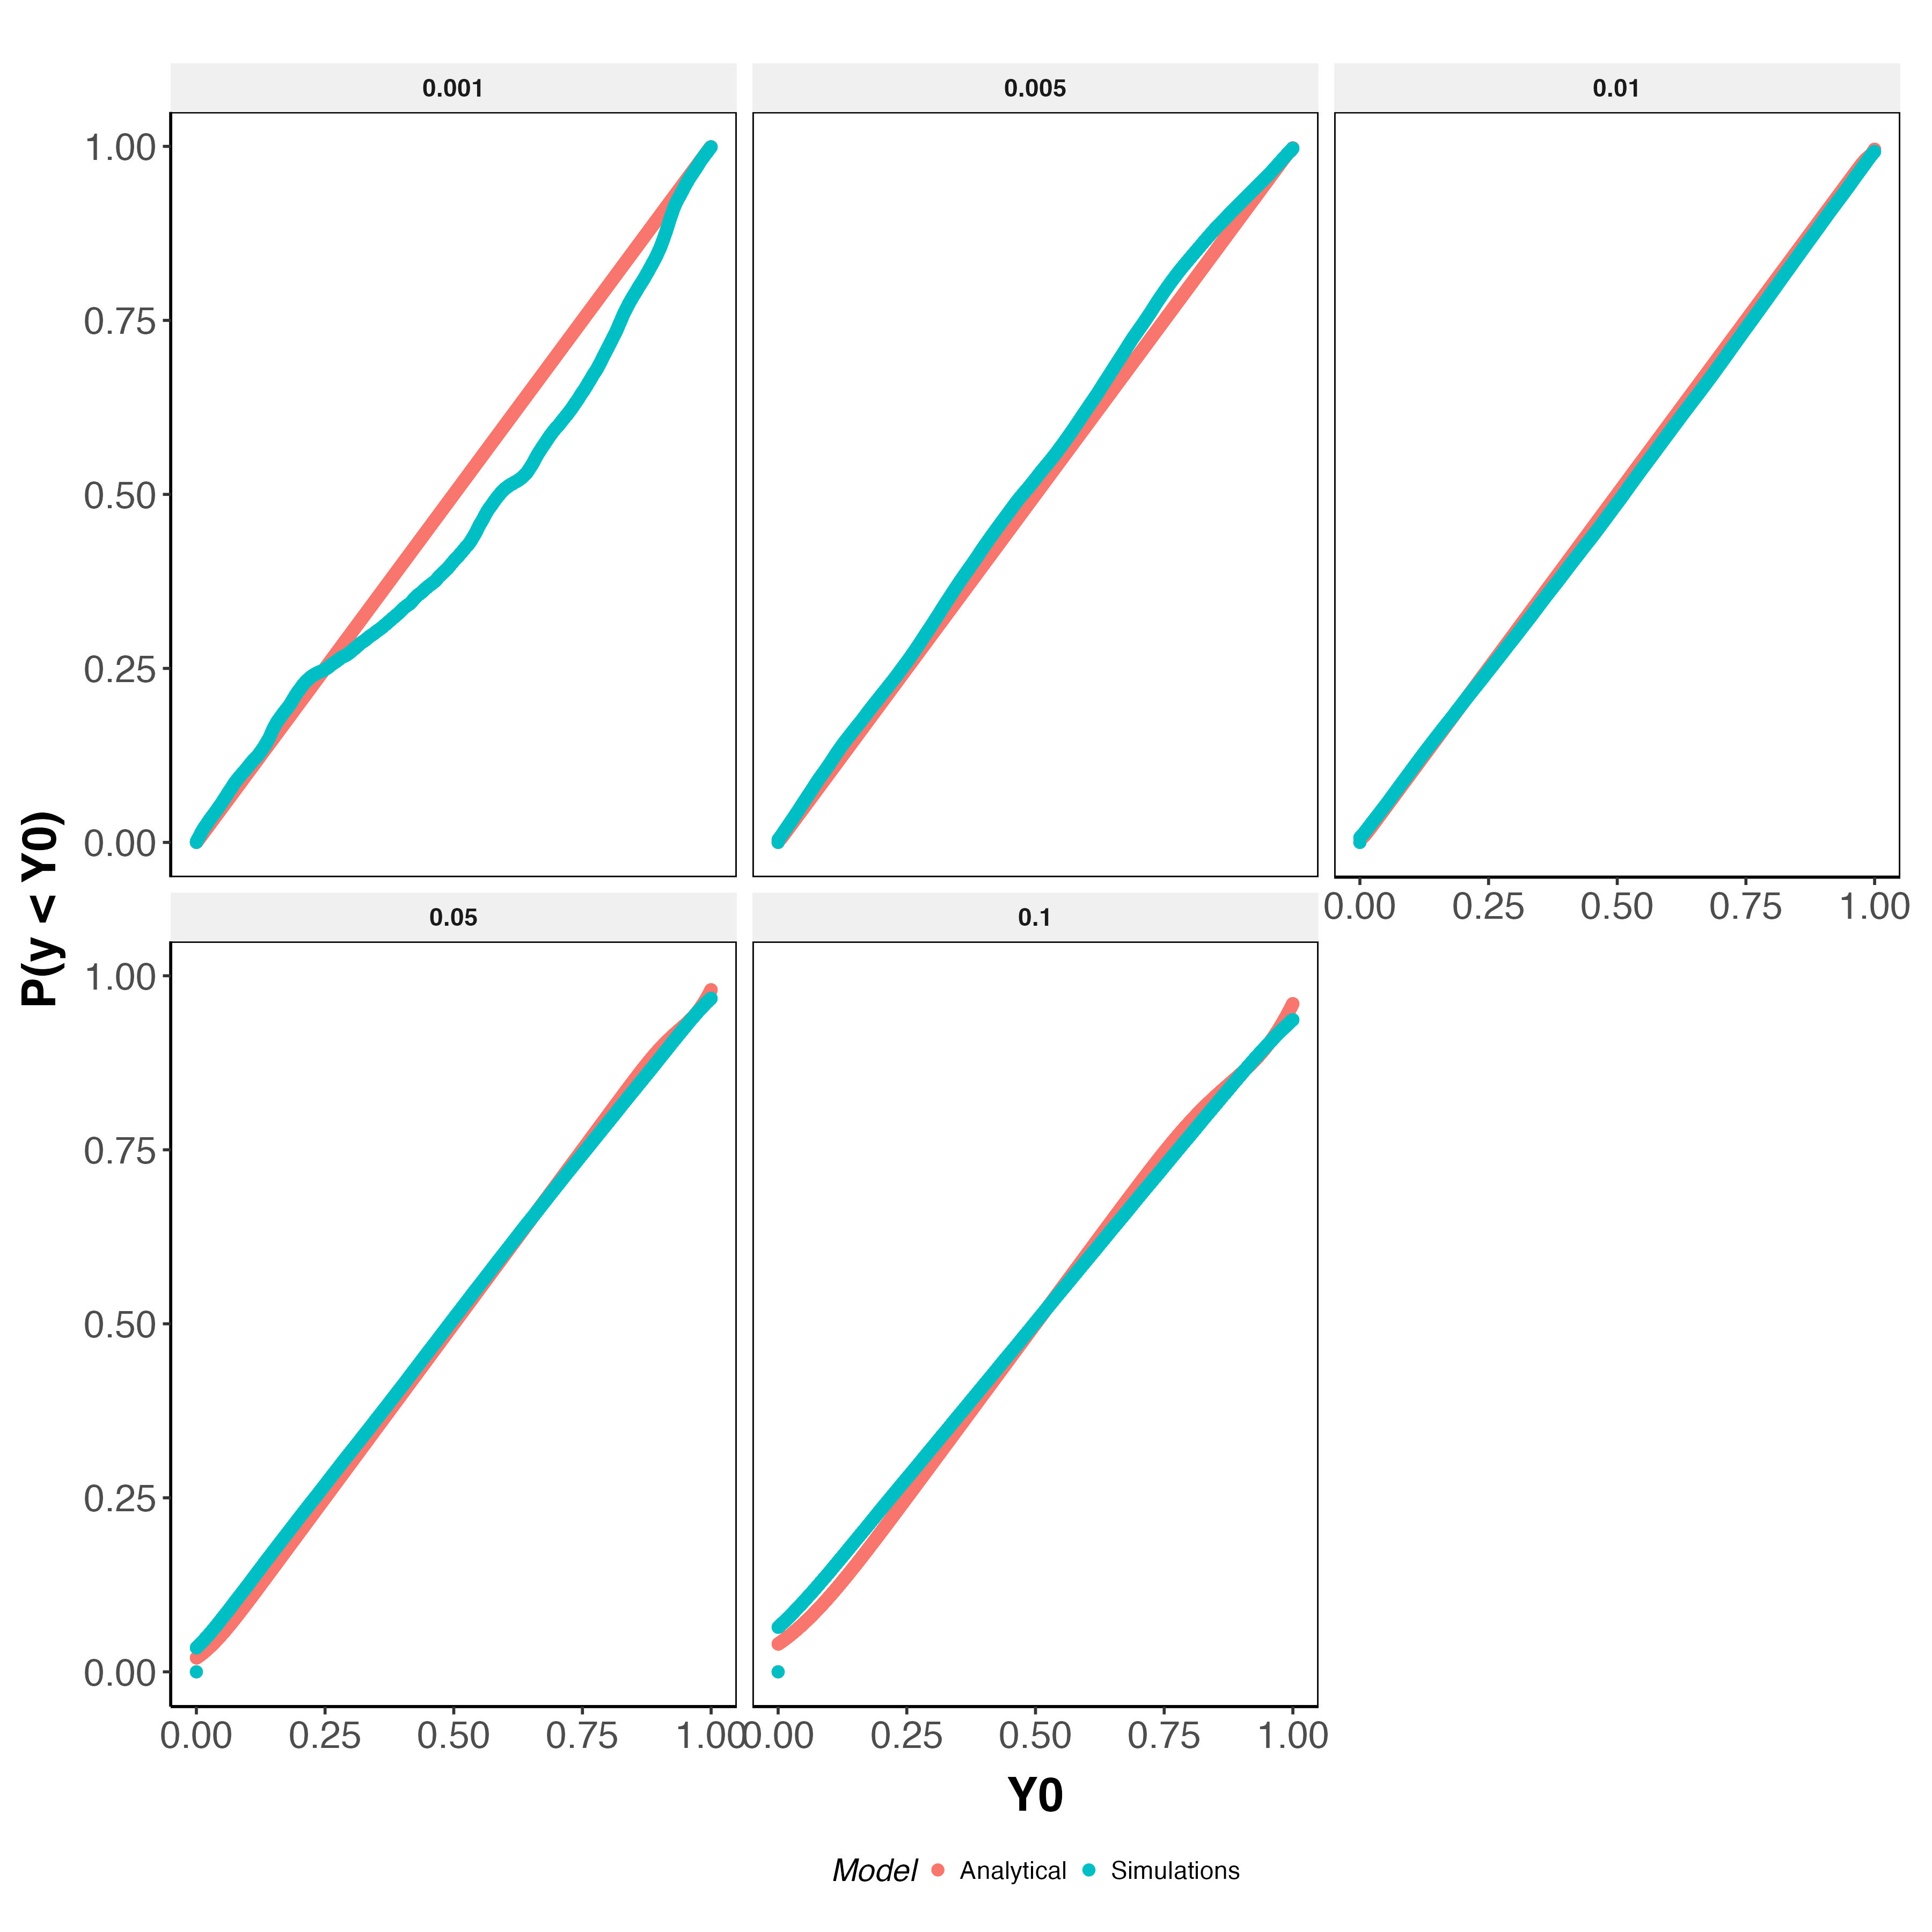
\includegraphics[width=\linewidth]{AditiveNoiseFigures/prob_dist_compare.jpg}
%     \caption{\textbf{Comparision of CDFs generated from simulations and the analytical calculations} Each panel shows the cumulative distribution obtained from Eq \ref{additiveCDF} (red) and numerically calculated trajectories (green). The CDFs agree well with each other, with minor differences that should not have any strong impact on sampling lambda values.} 
%     \label{fig:noiseDist}
% \end{figure}


\clearpage
\section{Supplementary Figures}

\begin{figure}[h!]
    \centering
    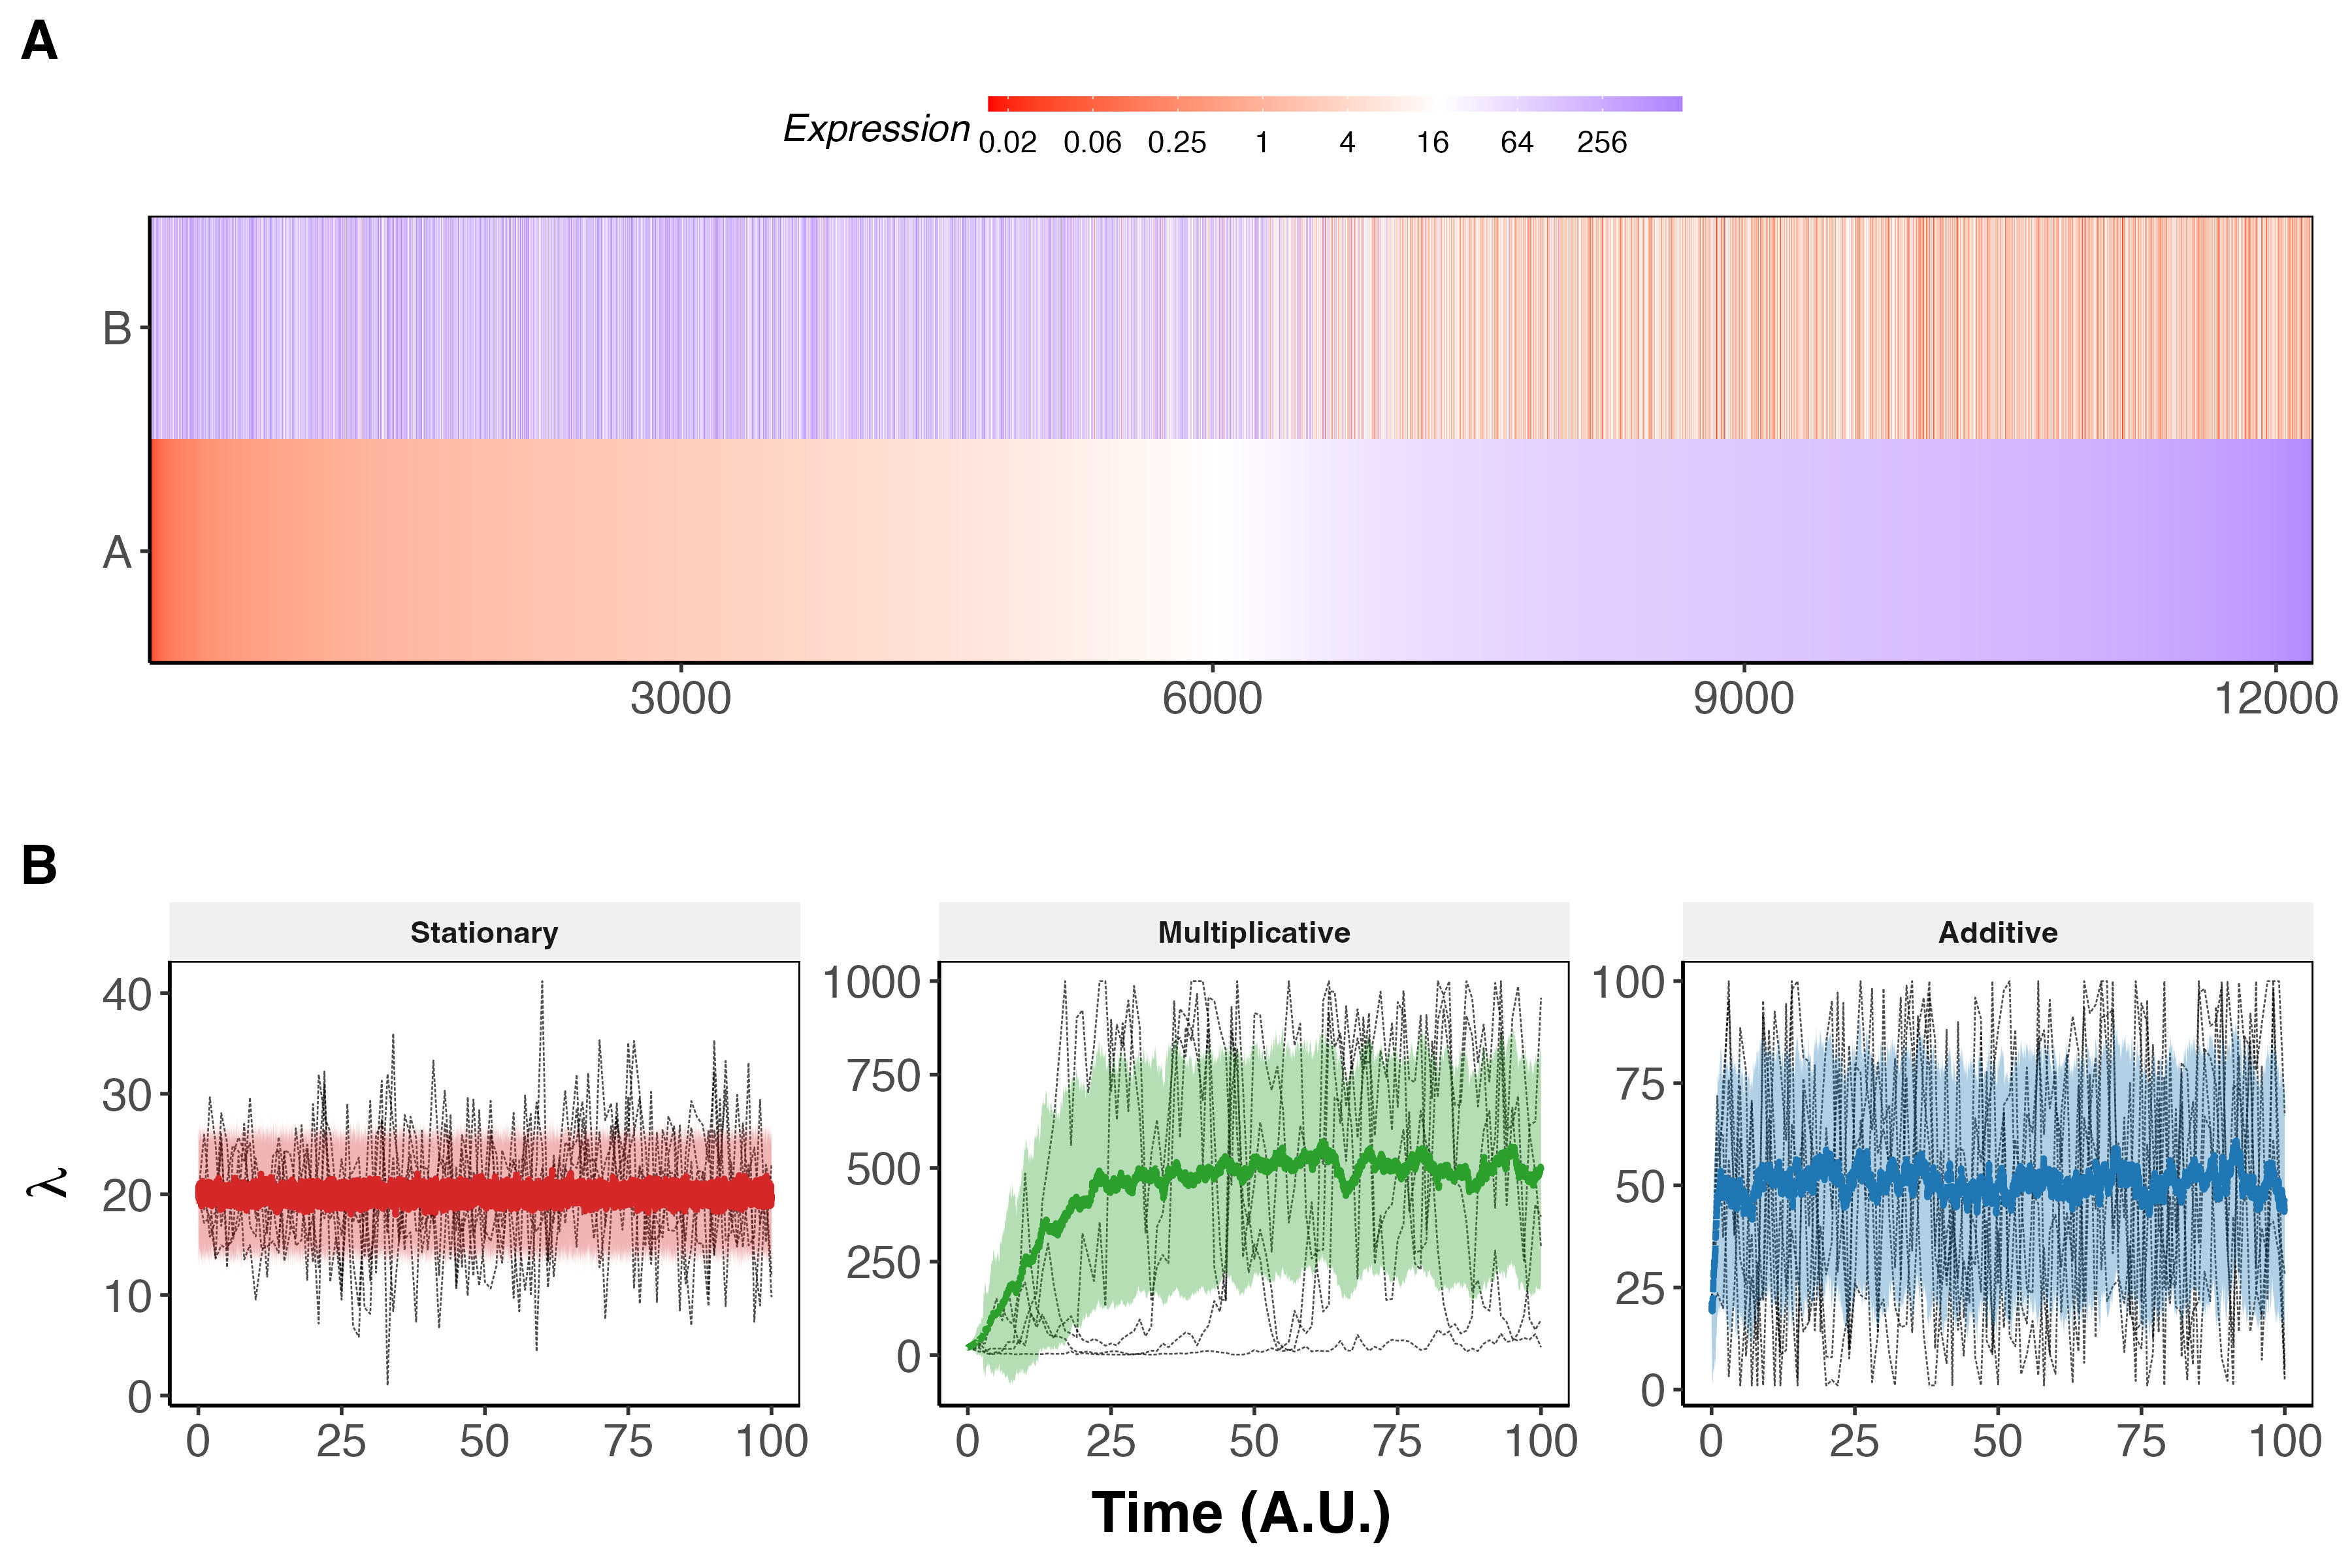
\includegraphics[width=0.8\linewidth]{Fig1S1.jpg}
    \caption{
    \textbf{(A)} Heatmap of RACIPE steady-state expression for nodes A and B in TS network, across all sampled parameter combinations. The steady states are sorted in increasing order of expression of node A. The color scale is in $log_2$ scale and centered at the mean of the two nodes' thresholds. \textbf{(B)} Same design as Figure~\ref{fig:1}D, but for a fold-change of an activatory edge ($\lambda_0 = 20$). Stationary and additive noise use $\lambda \in [1,100]$ with $\sigma_{\text{eff}} = 100\,\sigma$; multiplicative noise follows the geometric rule, $\lambda(t+dt) = \lambda(t)/(1+\sigma\eta)$ with $\lambda \in [1, 10^{3}]$, so $\lambda$ rises toward the maximal-strength bound (note the different $y$ scale).}
    \label{fig:1S1}
\end{figure}

\begin{figure}
    \centering
    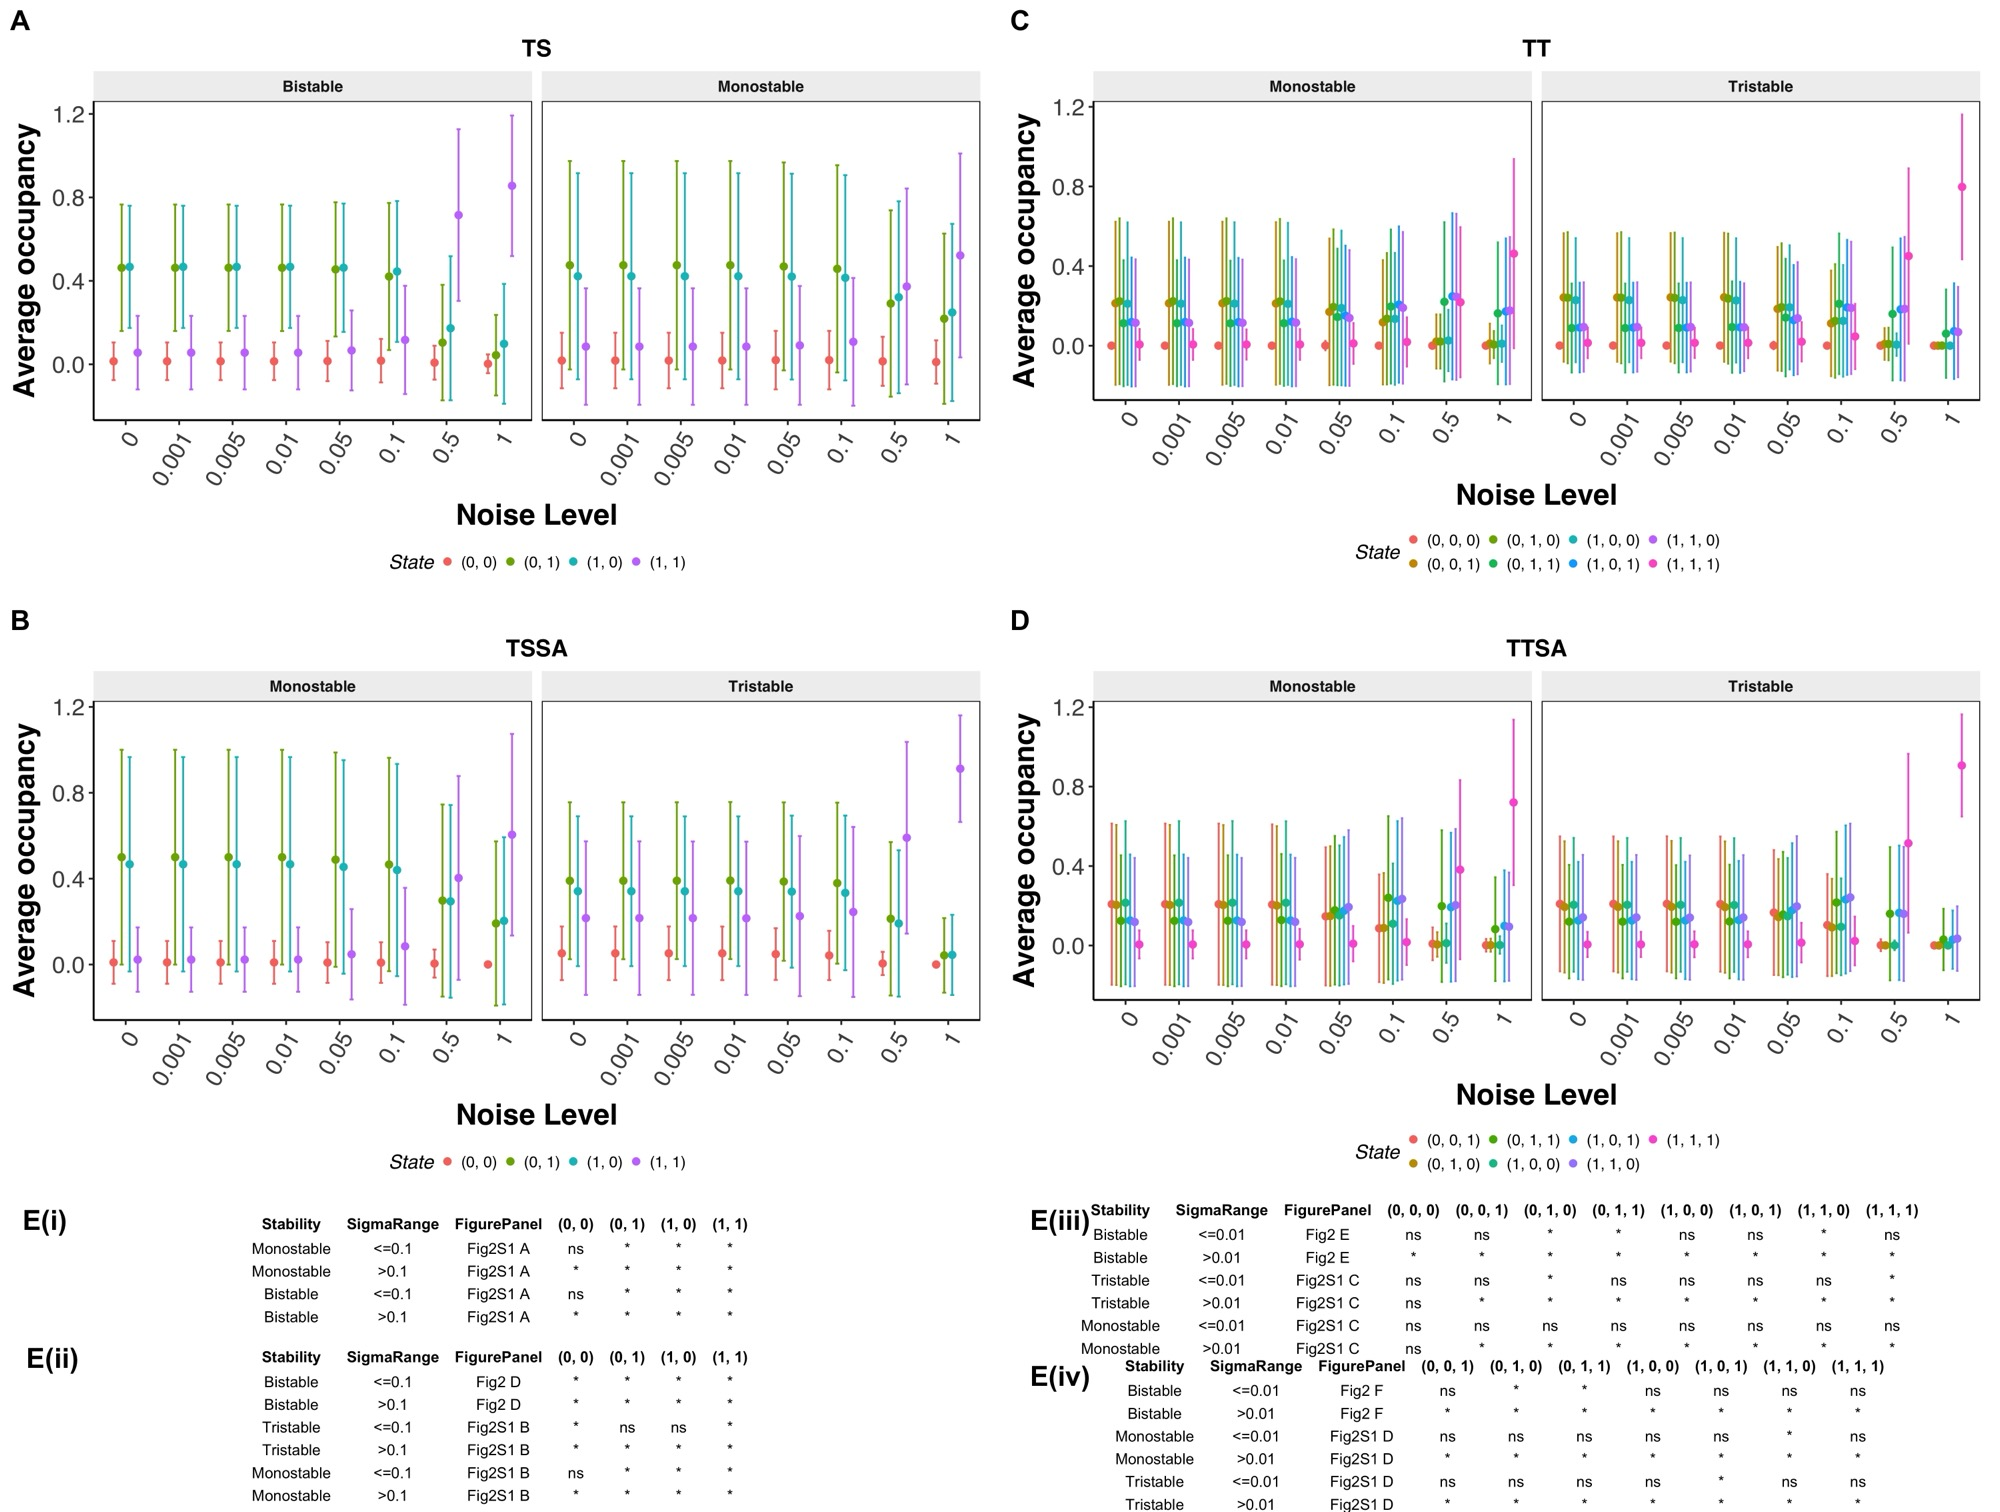
\includegraphics[width=0.8\linewidth]{Fig2S1.jpg}
    \caption{Occupancy vs.\ noise level, colored by discrete state, mean $\pm$ SD across parameter sets, for \textbf{(A)} TS (all parameter sets), \textbf{(B)} TSSA (monostable + tristable), \textbf{(C)} TT (monostable + tristable), and \textbf{(D)} TTSA (monostable + tristable).}
    \label{fig:2S1}
\end{figure}

\begin{figure}
    \centering
    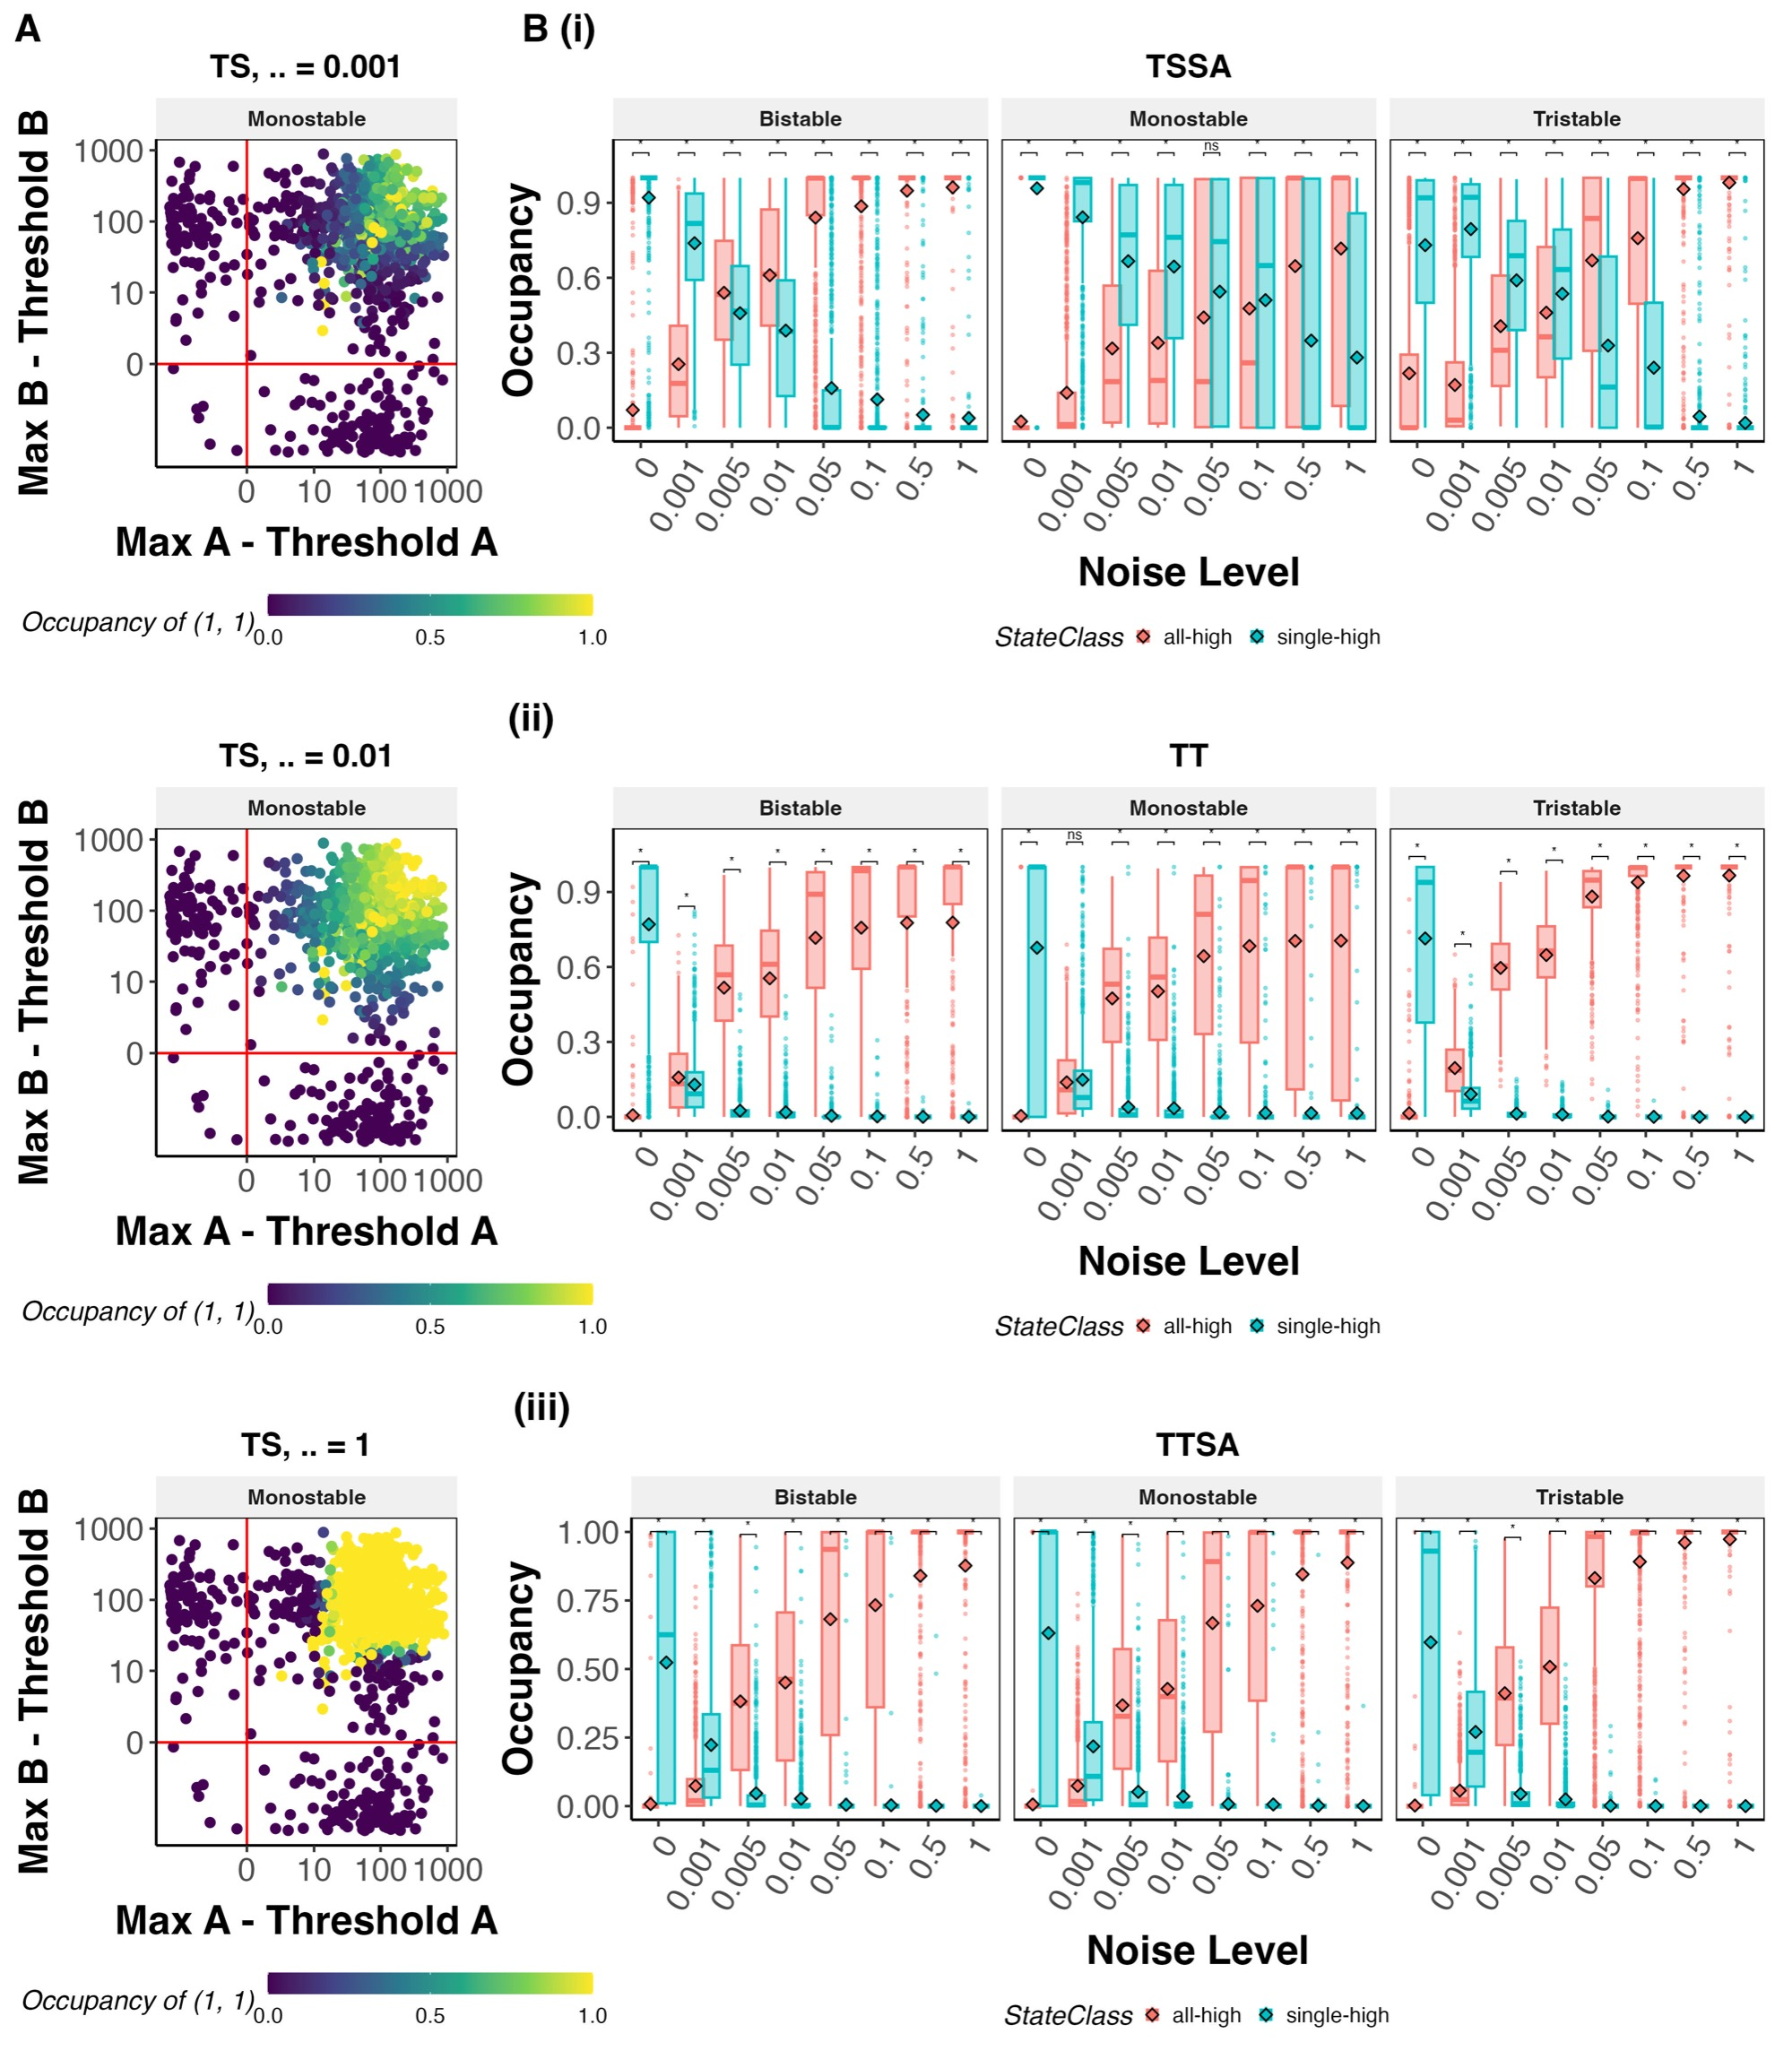
\includegraphics[width=0.8\linewidth]{Fig3S1.jpg}
    \caption{\textbf{(A)} Occupancy boxplots (as in Fig.\ 3B) for TSSA, TT, and TTSA, stacked vertically. \textbf{(B)} Reachability scatter (as in Figure~\ref{fig:3}C) for the TS network at $\sigma = 0.001, 0.01, 1.0$ (the noise levels not shown in the main figure), stacked vertically. \textbf{(C)} Reachability scatter for the TSSA network at $\sigma = 0.001, 0.01, 0.1, 1.0$.}
    \label{fig:3S1}
\end{figure}

\begin{figure}
    \centering
    \begin{minipage}{0.49\linewidth}\centering \textbf{(A)} TS\\ 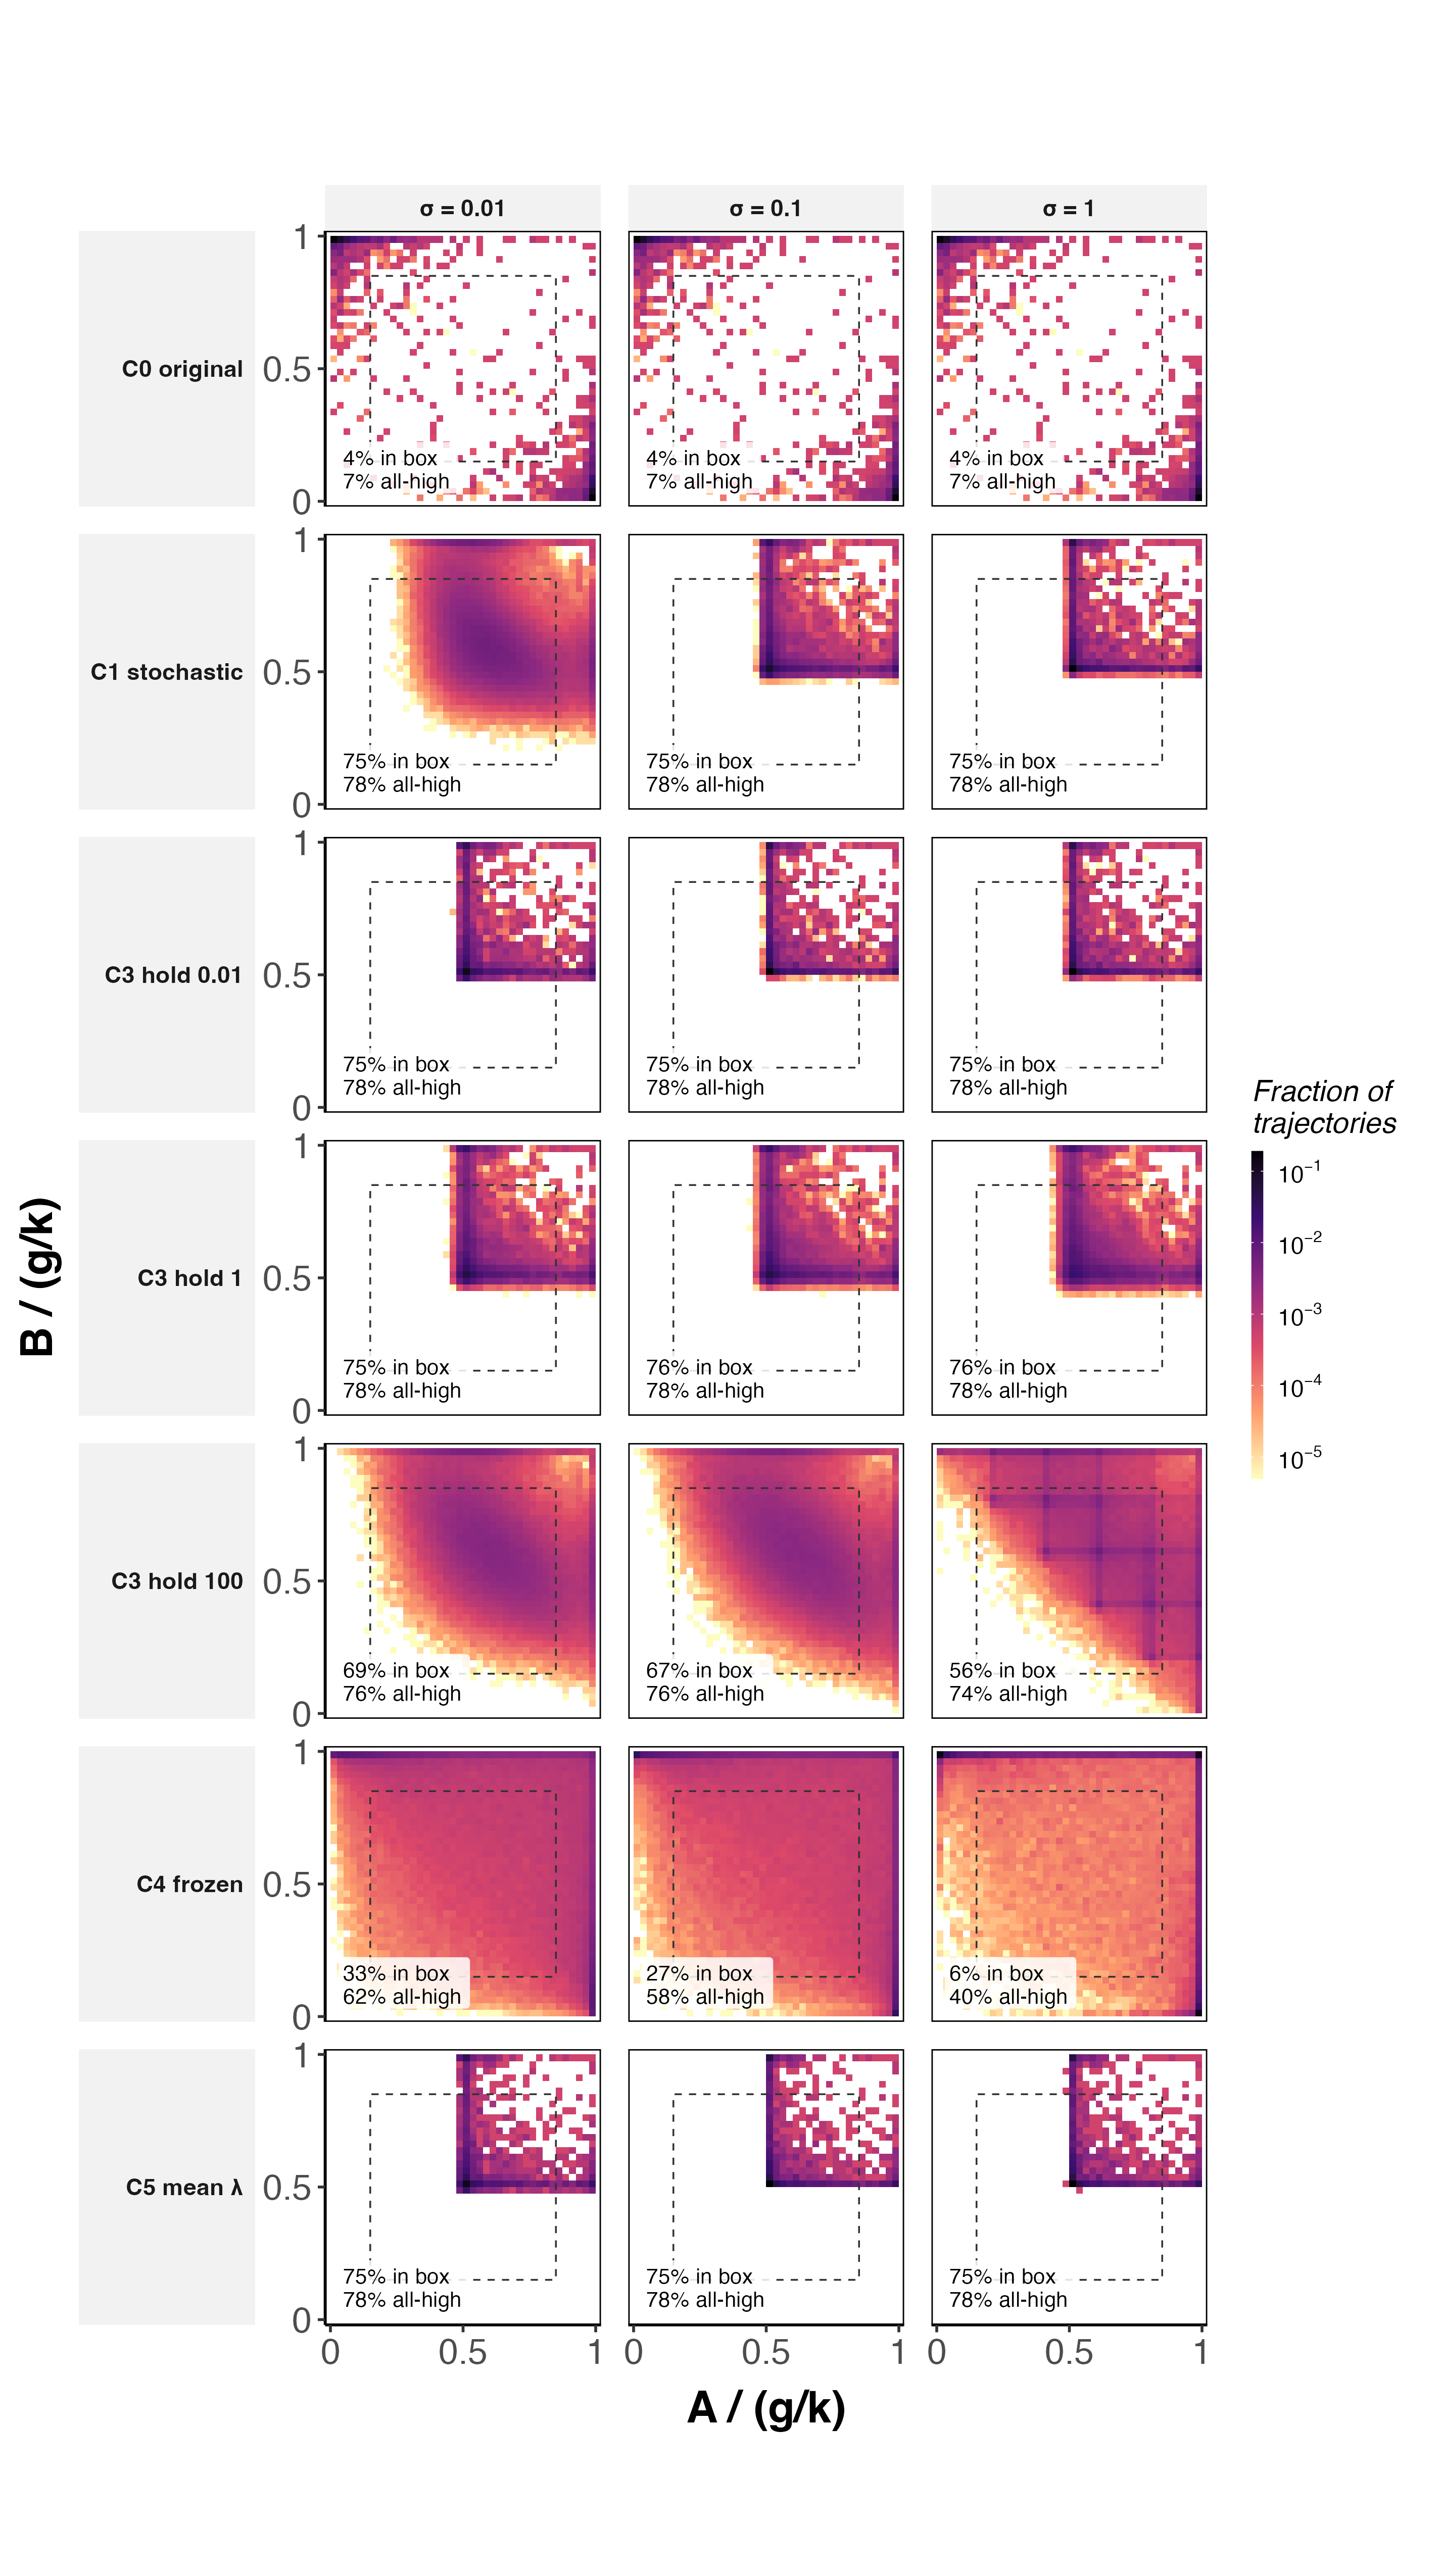
\includegraphics[width=\linewidth]{FigS_expr_joint_TS.png}\end{minipage}
    \begin{minipage}{0.49\linewidth}\centering \textbf{(B)} TT\\ 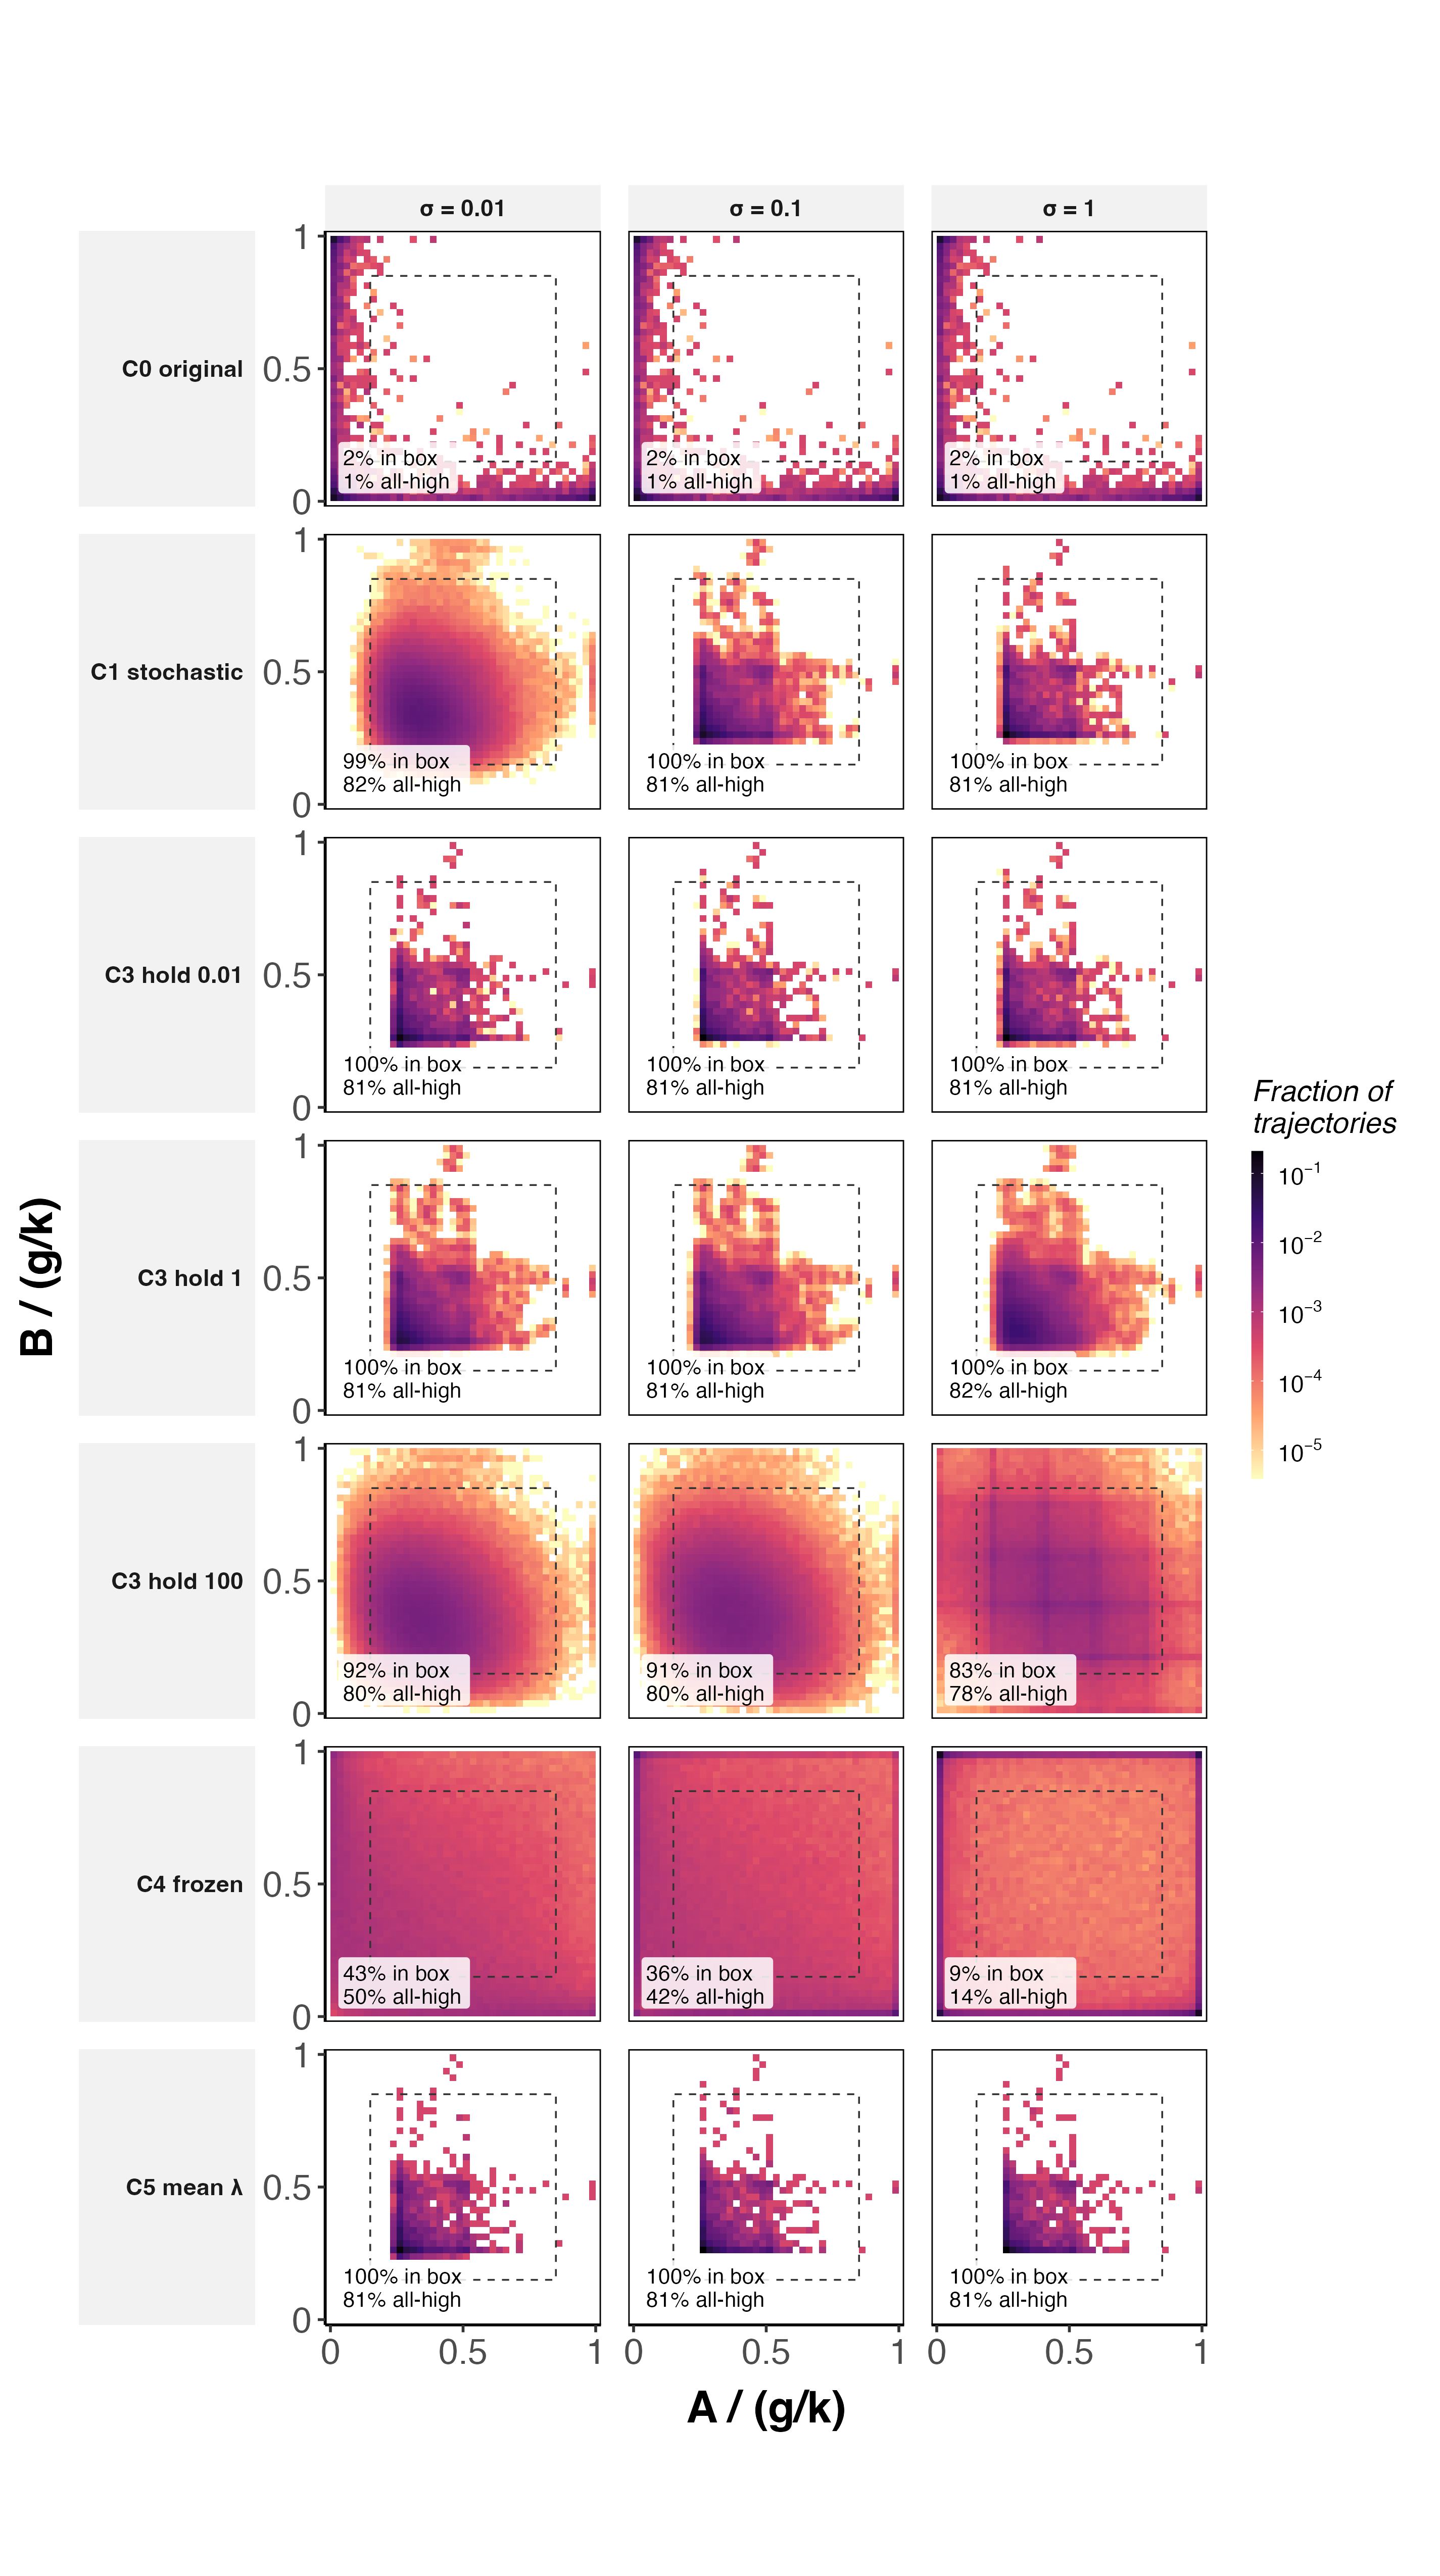
\includegraphics[width=\linewidth]{FigS_expr_joint_TT.png}\end{minipage}
    \caption{\textbf{Expression levels behind the discrete states, additive noise.} Joint time-averaged expression of nodes A and B per trajectory, as a fraction of each parameter set's maximum ($g/k$), for \textbf{(A)} TS and \textbf{(B)} TT (node C not shown). Rows: control conditions (Section~\ref{sec:controls}); C0 is repeated in every column. Columns: $\sigma = 0.01$, 0.1, 1 at $\Delta t = 0.01$. Colour: fraction of trajectories per bin (log scale). Dashed box: both nodes at intermediate levels (0.15--0.85 of maximum). Numbers give the fraction of trajectories inside the box and the fraction classified as all-high by the discretization thresholds. Under stochastic noise (C1), fast hold-resampling (C3, hold 0.01 and 1) and the mean-$\lambda$ control (C5), expression sits on the floor set by the average fold change (about 0.5 of maximum in TS, 0.25 in TT); the frozen control (C4) spreads expression over the full range.}
    \label{fig:3S_expr}
\end{figure}

\begin{figure}
    \centering
    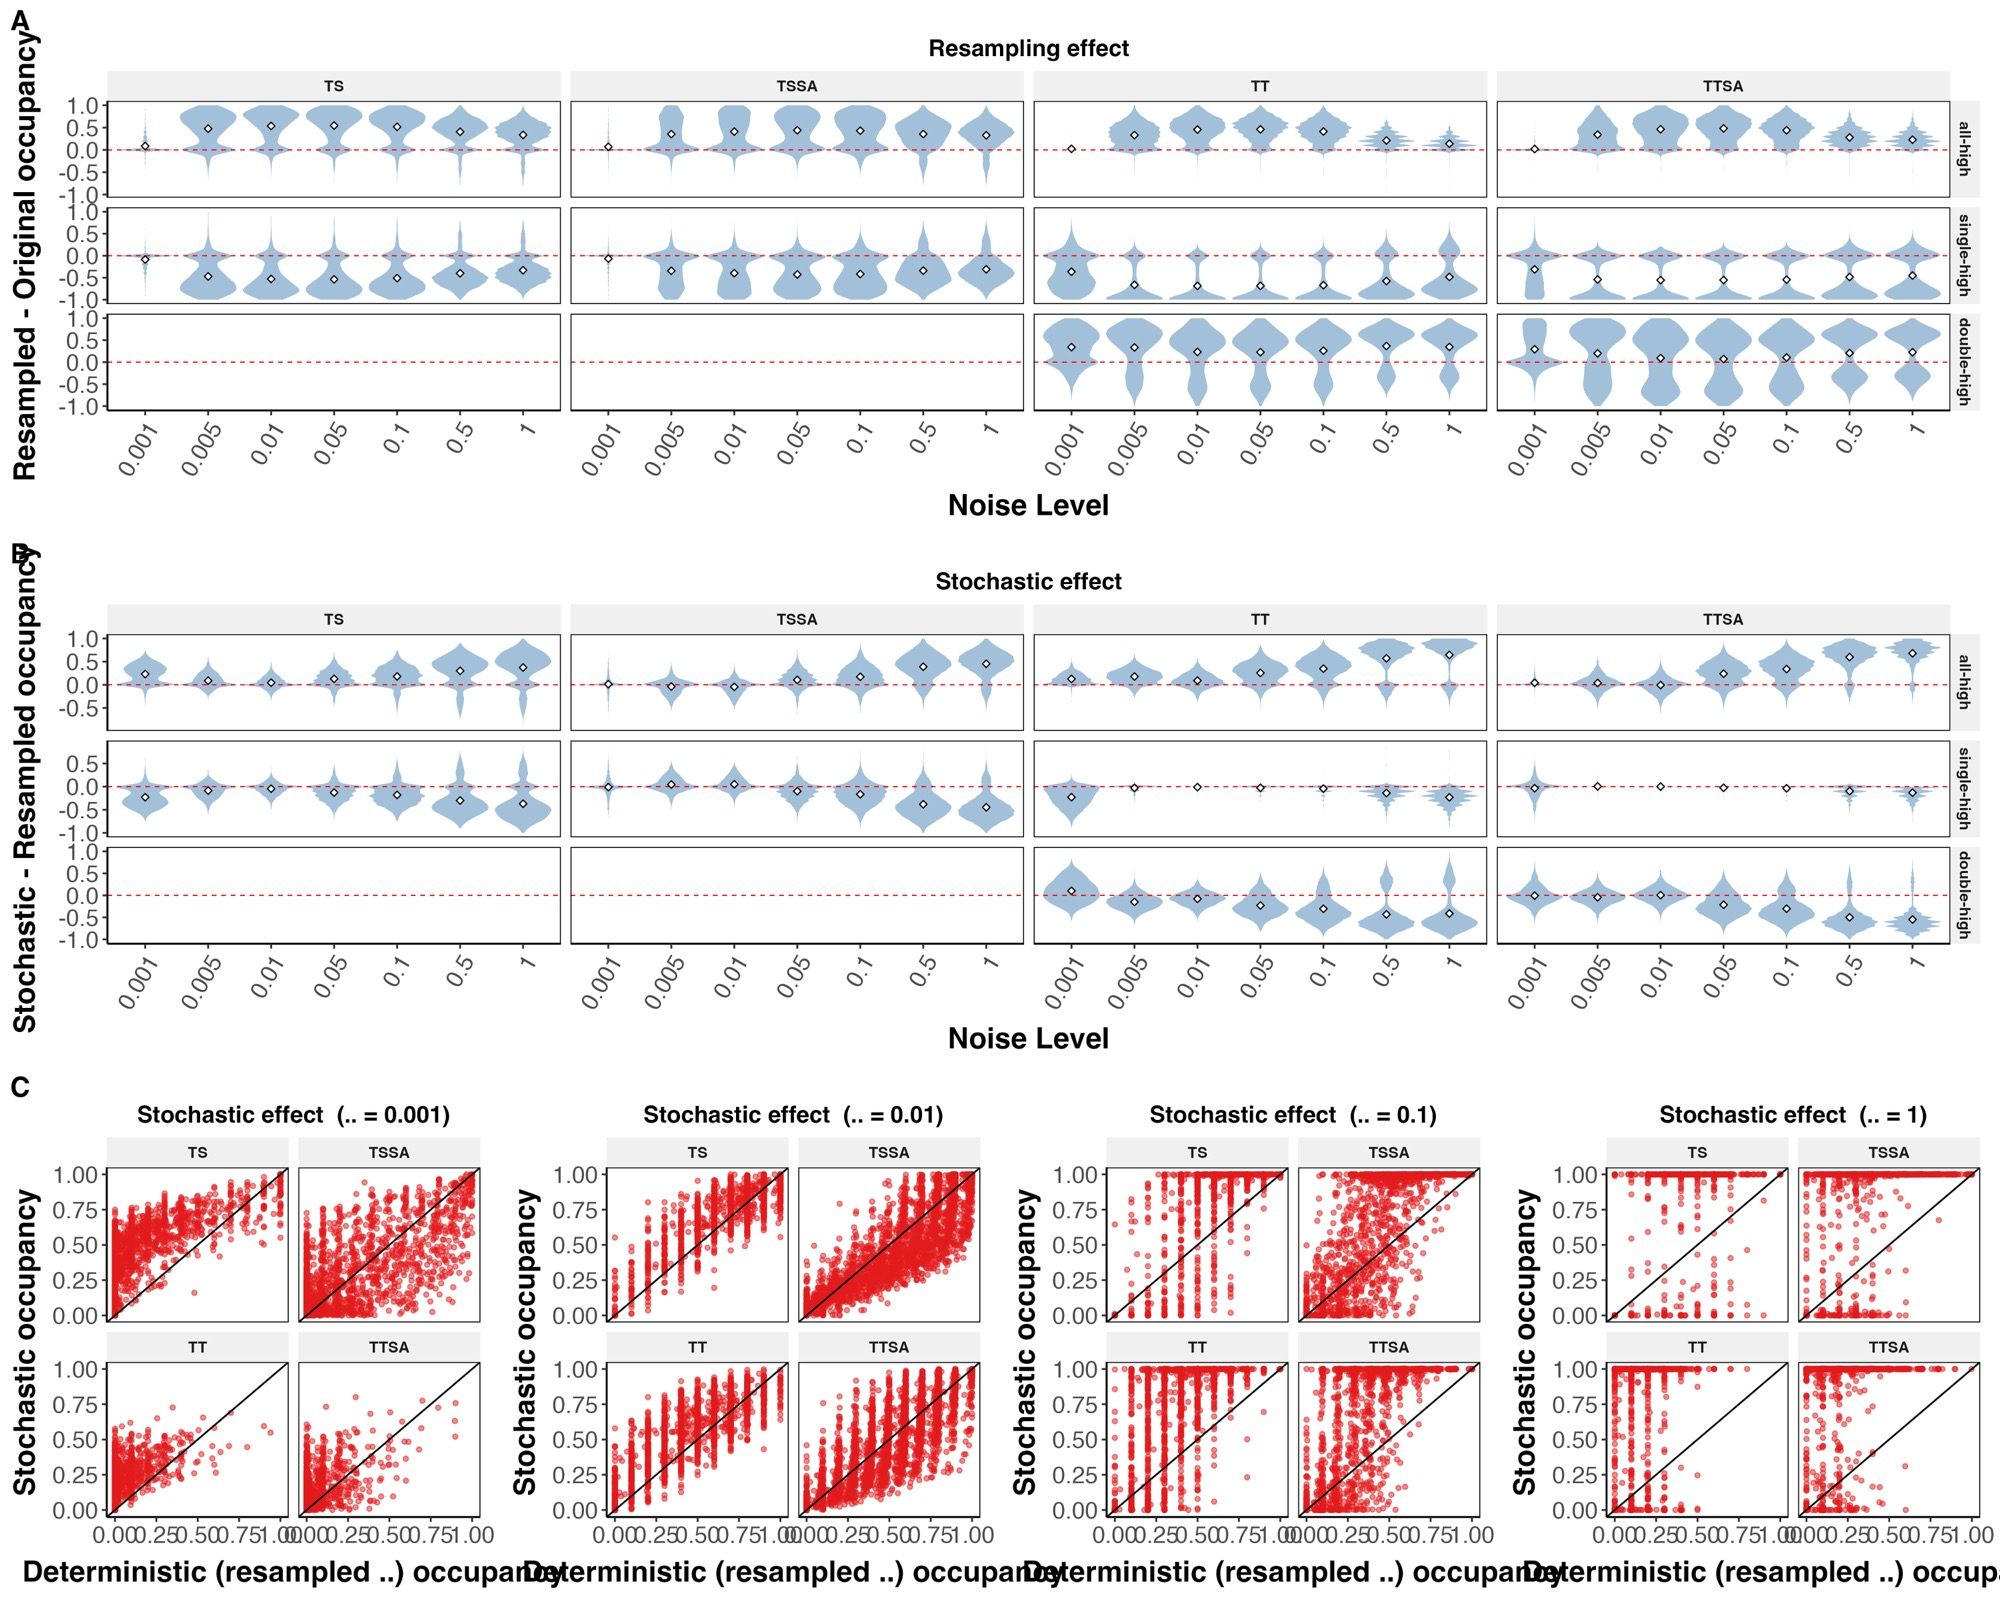
\includegraphics[width=0.8\linewidth]{Fig4S1.jpg}
    \caption{\textbf{(A)} Resampling effect (as in Figure~\ref{fig:3b}B), collapsed to a single per-parameter-set difference and shown across all noise levels, faceted by state class (all-high/single-high/double-high) and network (TS, TSSA, TT, TTSA). \textbf{(B)} Same, for the stochastic effect. \textbf{(C)} Paramwise scatter of resampled-$\lambda$ deterministic vs.\ stochastic occupancy of the all-high state, all four networks, at each of four noise levels (0.001, 0.01, 0.1, 1.0).}
    \label{fig:3bS1}
\end{figure}

\begin{figure}
    \centering
    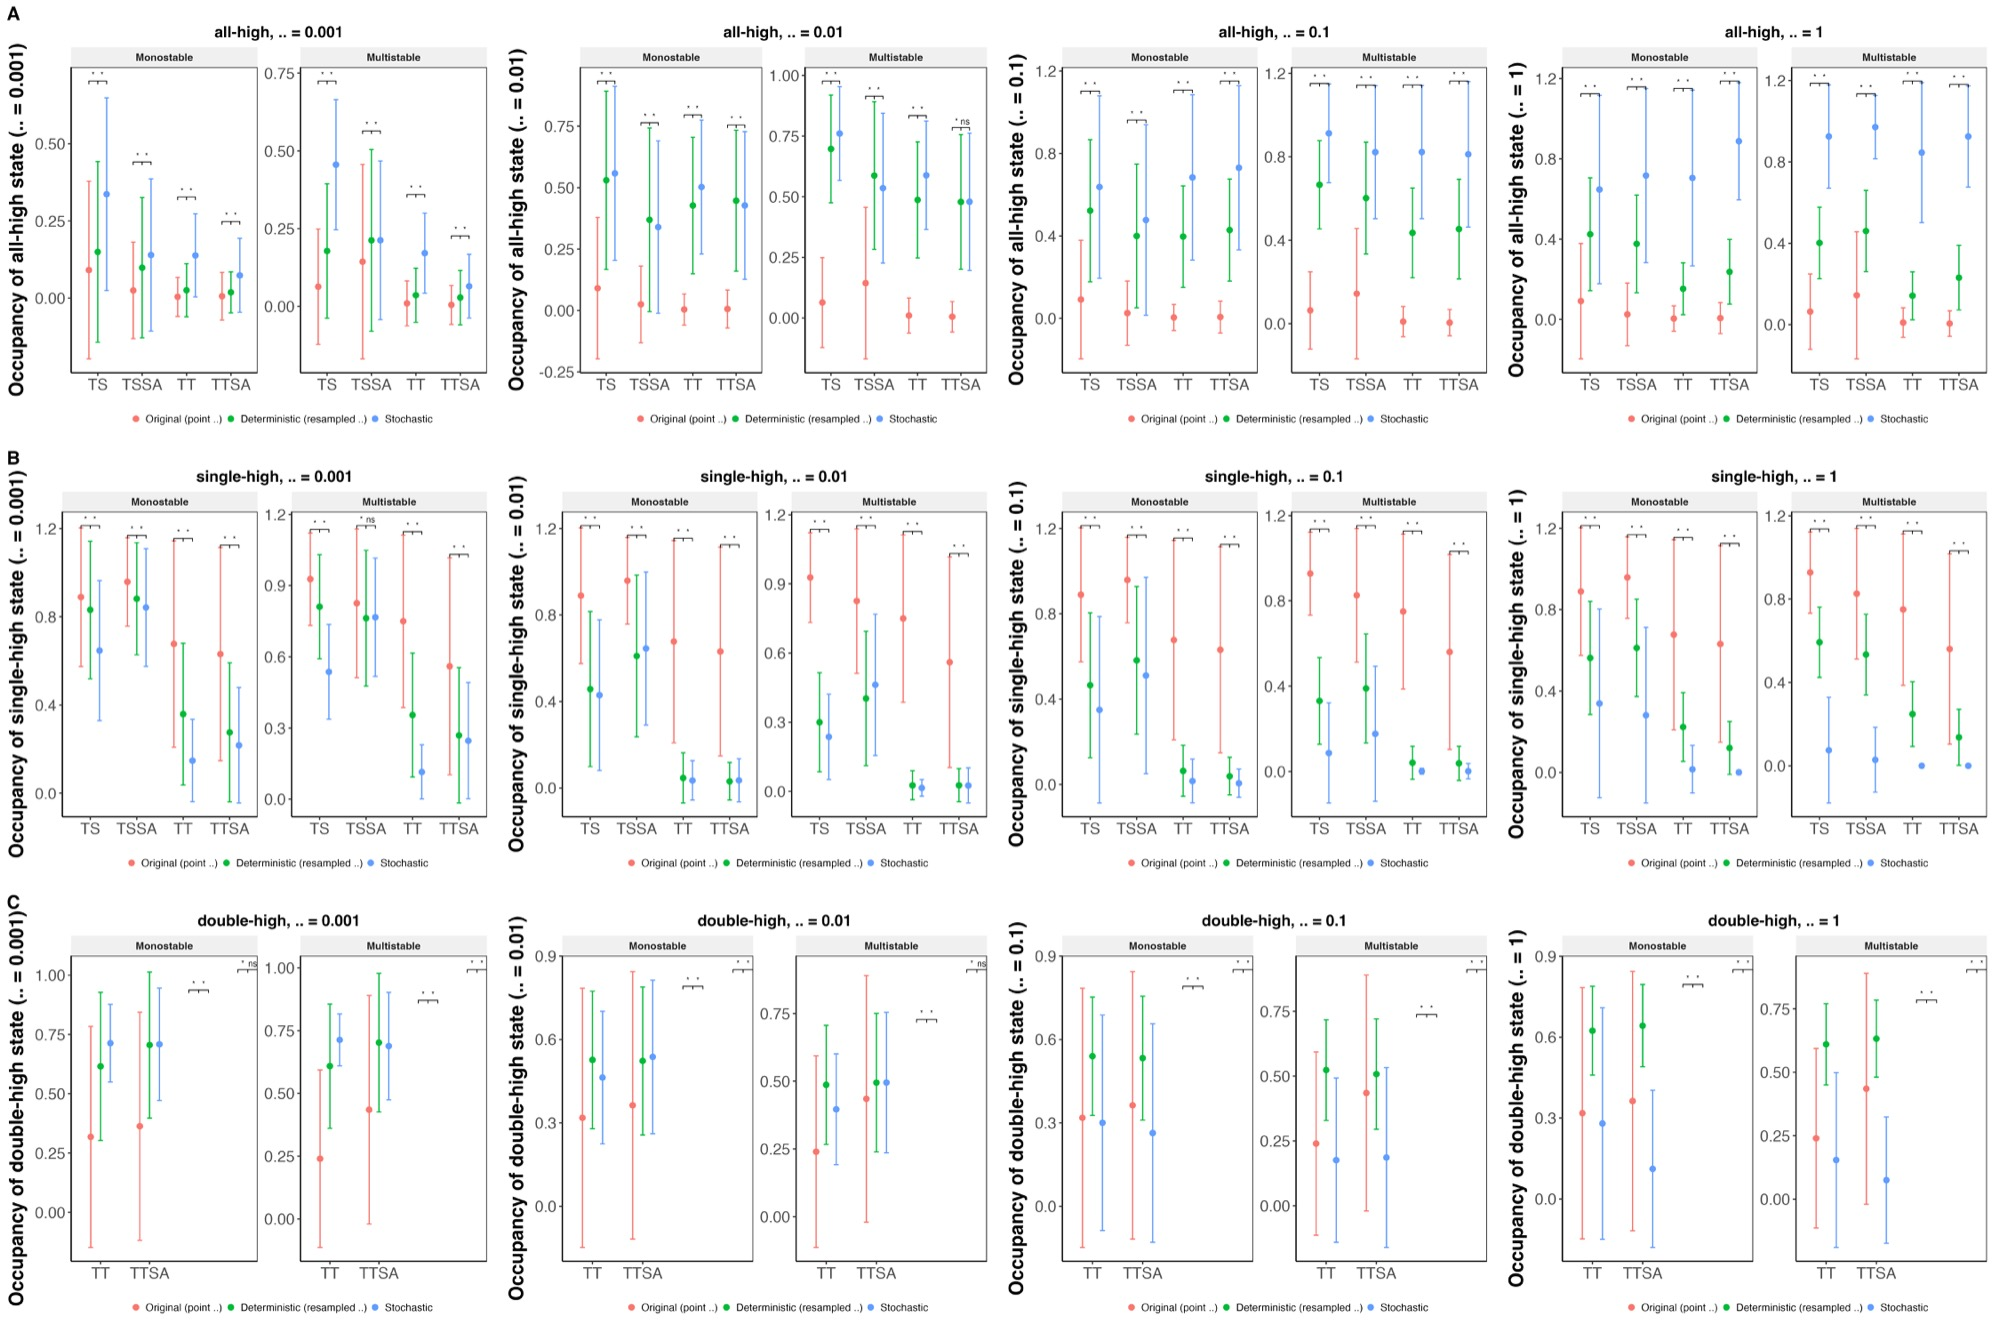
\includegraphics[width=0.8\linewidth]{Fig4S2.jpg}
    \caption{All-high \textbf{(A)}, single-high \textbf{(B)}, and double-high \textbf{(C)} state occupancy comparisons (as in Figure~\ref{fig:3b}D: original/resampled/stochastic, faceted by stability class), repeated at four noise levels (columns: 0.001, 0.01, 0.1, 1.0), for TS, TSSA, TT, TTSA. 2-node networks (TS, TSSA) have no double-high state distinct from all-high, so they are absent from that row.
}
    \label{fig:3bS2}
\end{figure}

\begin{figure}
    \centering
    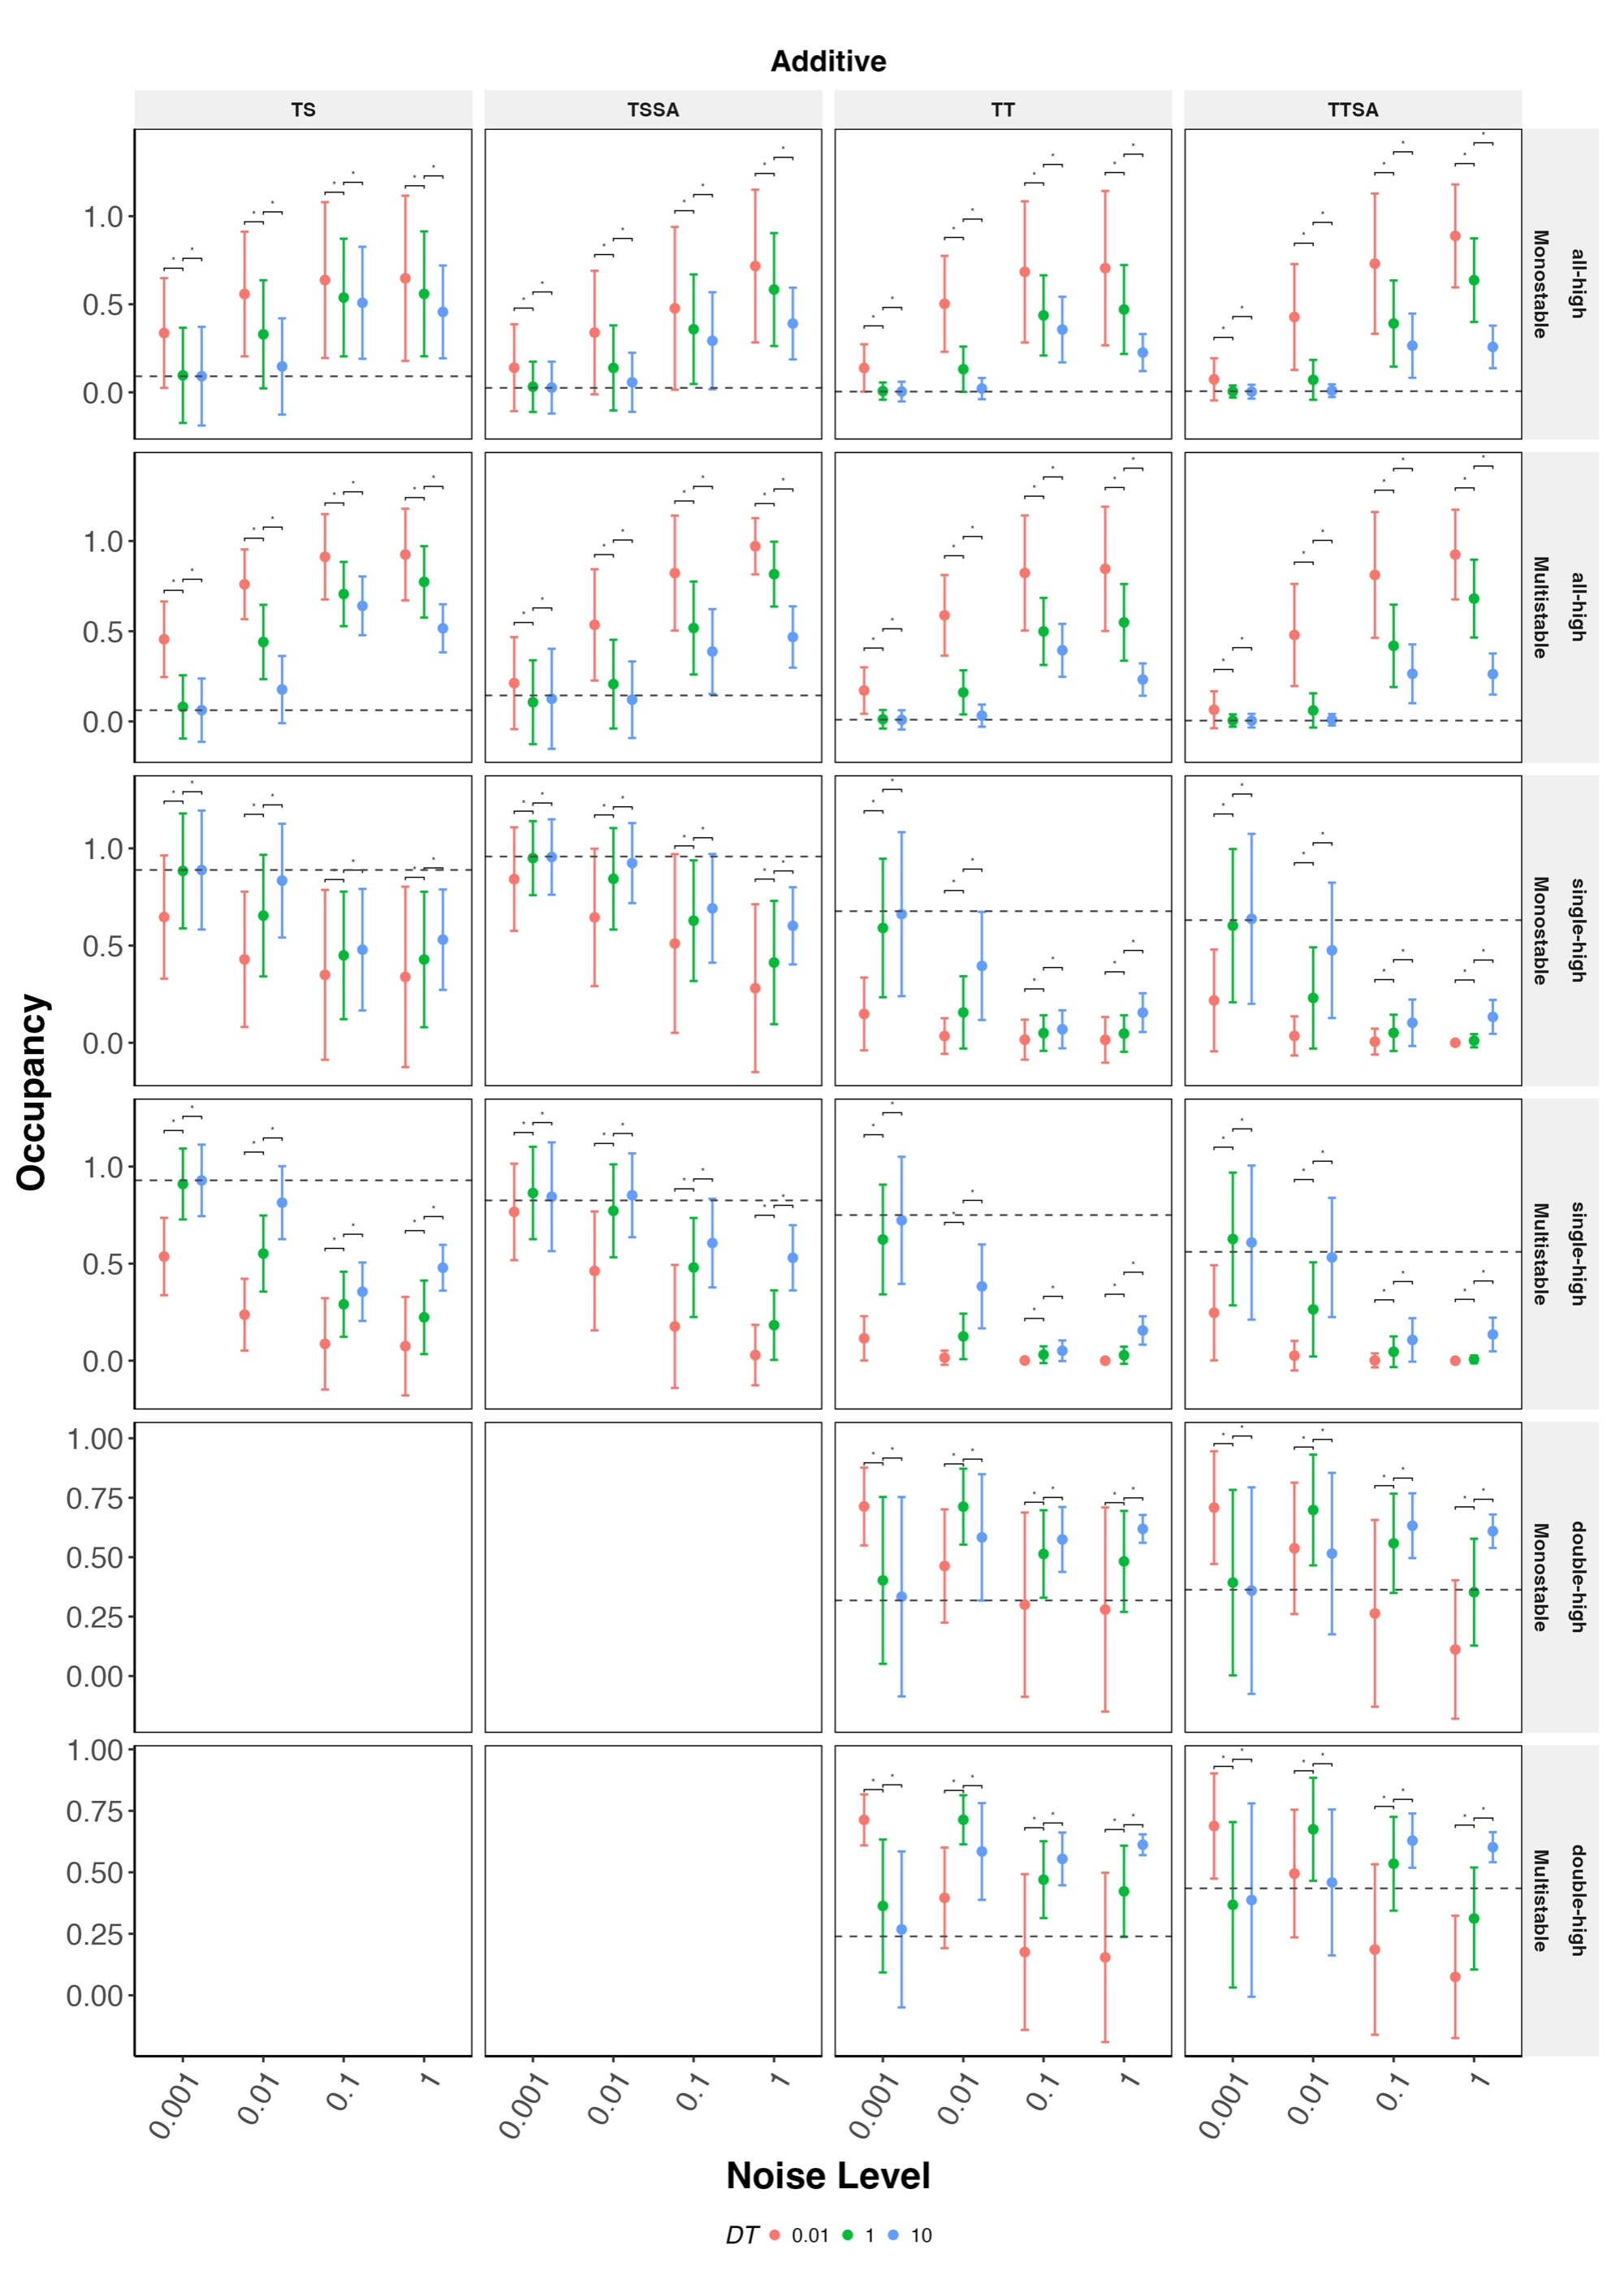
\includegraphics[width=0.8\linewidth]{Fig4S3.jpg}
    \caption{Comparison of occupancies for additive noise simulated at different values of $dt$}
    \label{fig:3bS3}
\end{figure}

\begin{figure}
    \centering
    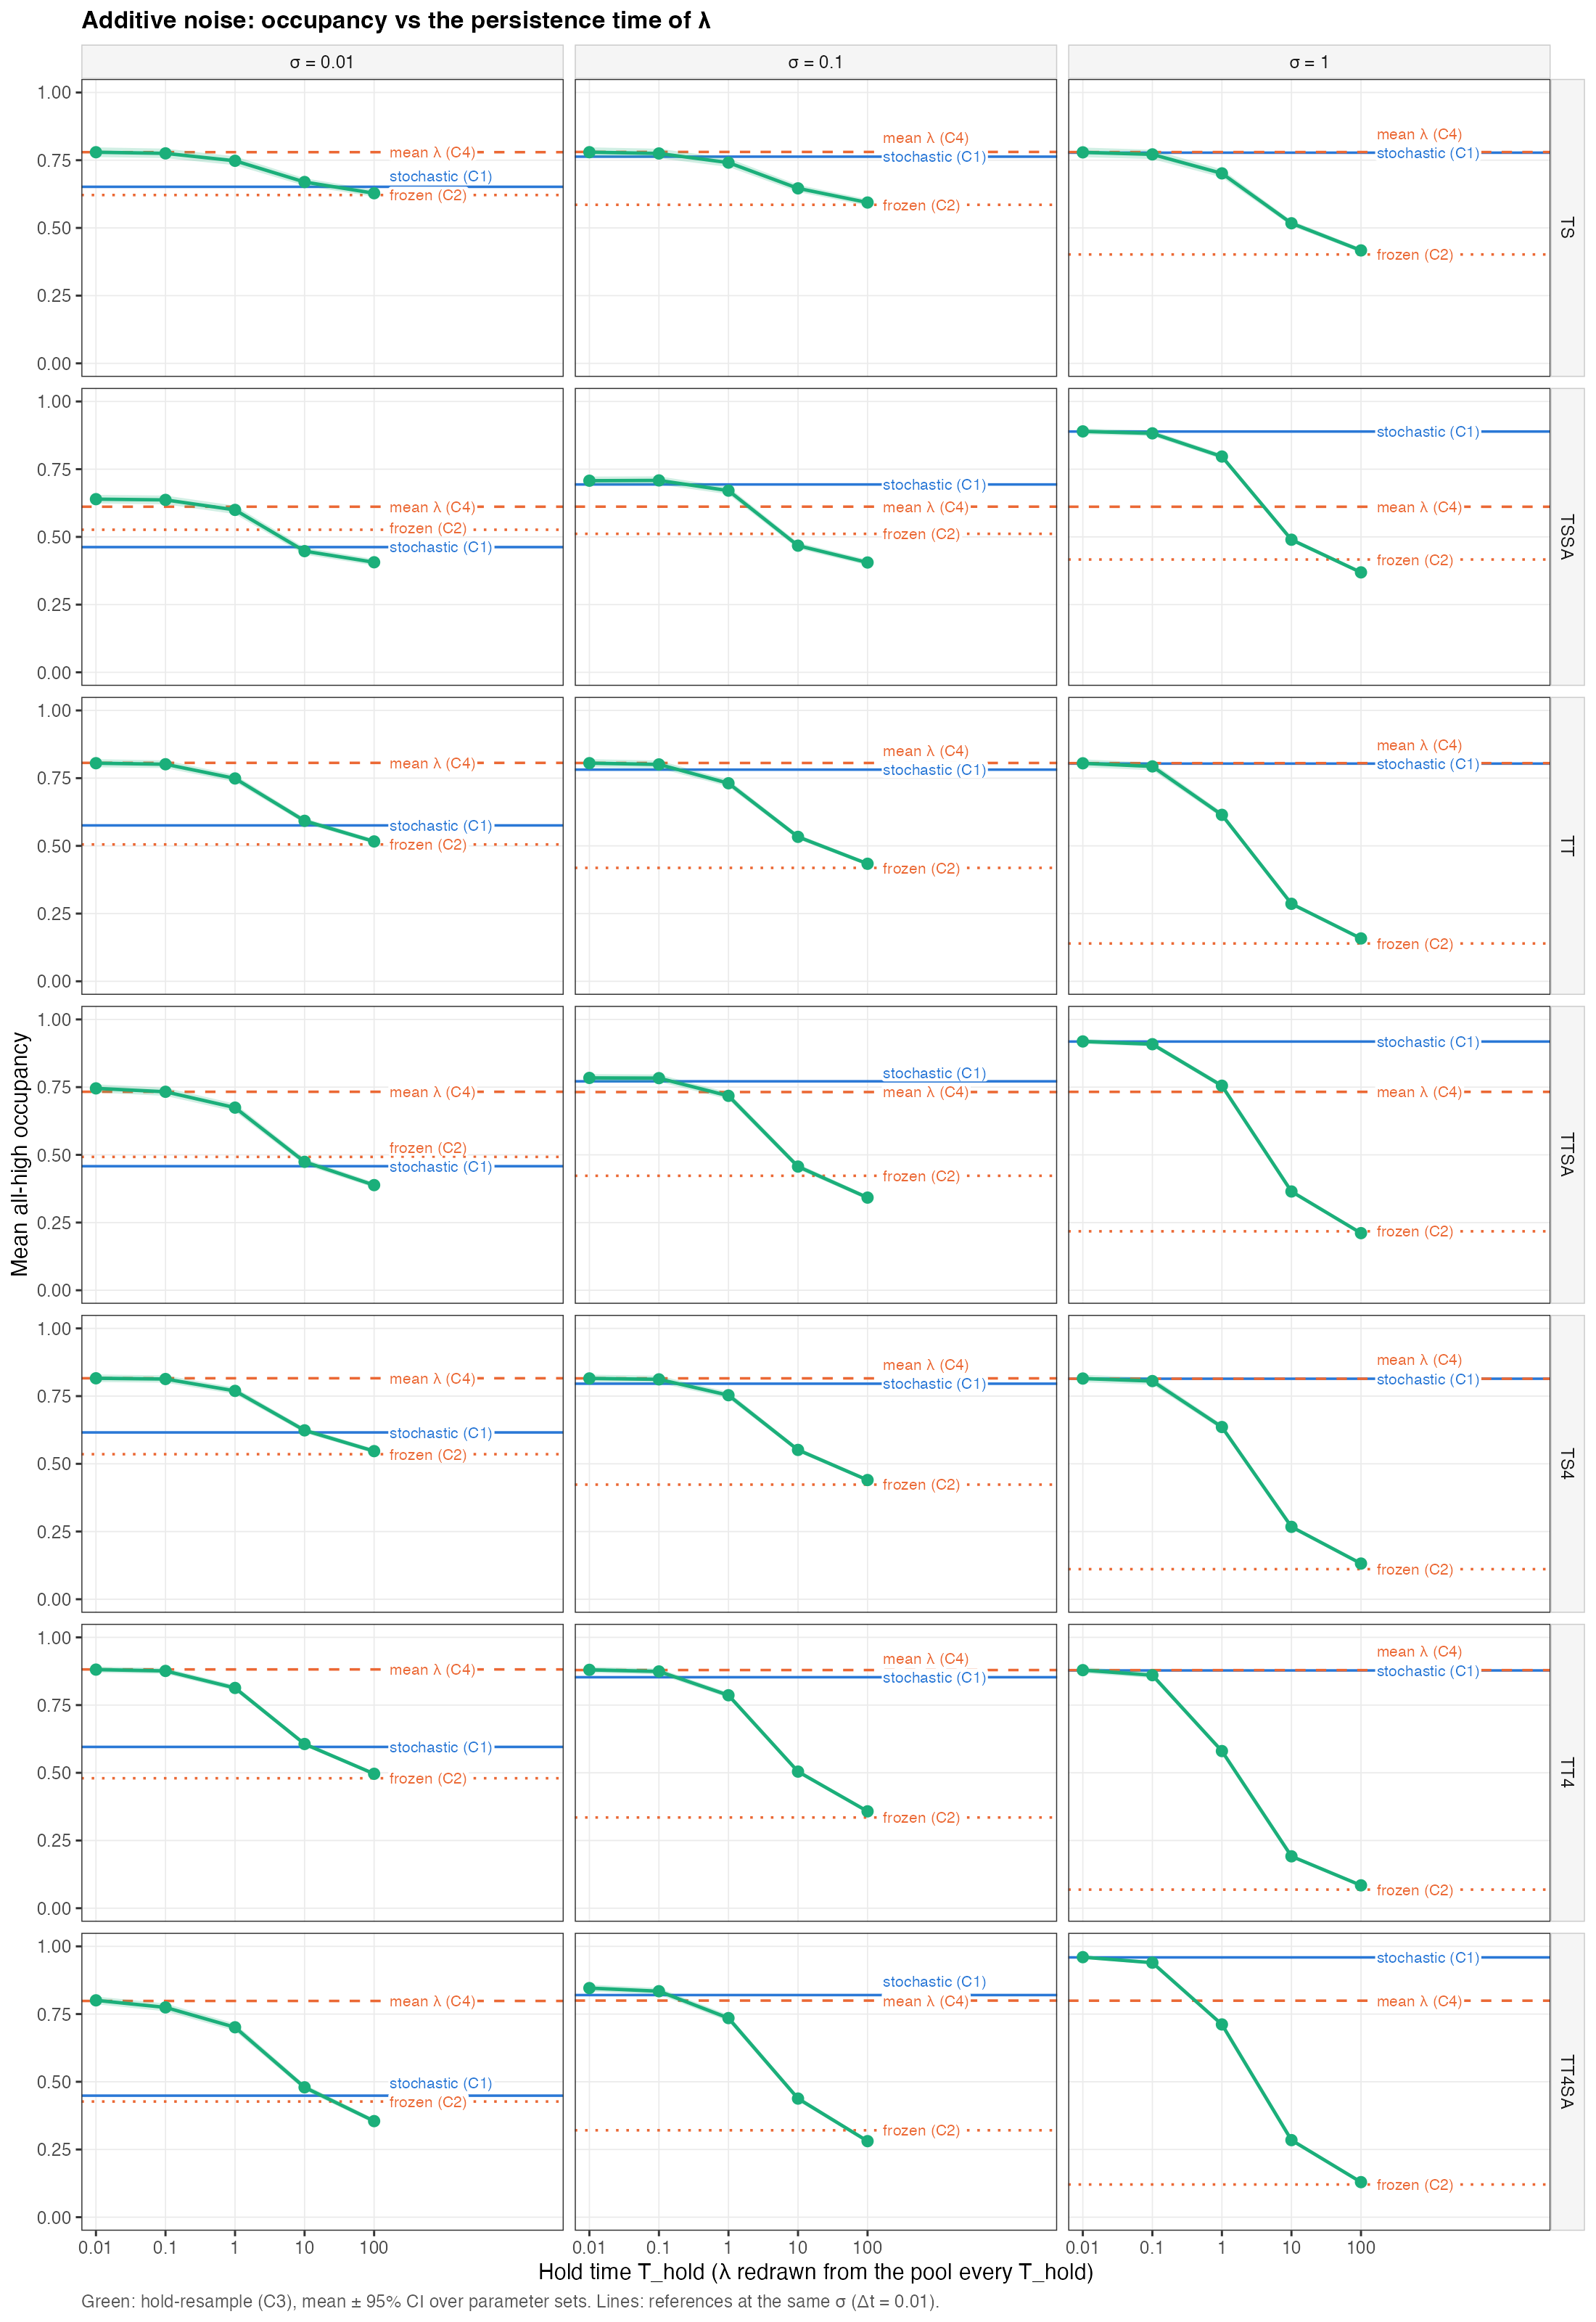
\includegraphics[width=0.85\linewidth]{FigS_ladder_addi.png}
    \caption{\textbf{Additive noise: occupancy versus the persistence time of $\lambda$ at fixed distribution.} Mean all-high occupancy under the hold-resample control C3 (green; mean $\pm$ 95\% CI over parameter sets), in which $\lambda$ is drawn from the values visited by the stochastic simulation and redrawn every $T_\text{hold}$. Lines show the stochastic simulation (C1, blue), the mean-$\lambda$ control (C4, dashed) and frozen draws (C2, dotted) at the same $\sigma$ ($dt = 0.01$). Rows, networks; columns, $\sigma$.}
    \label{fig:S_ladder}
\end{figure}

\begin{figure}
    \centering
    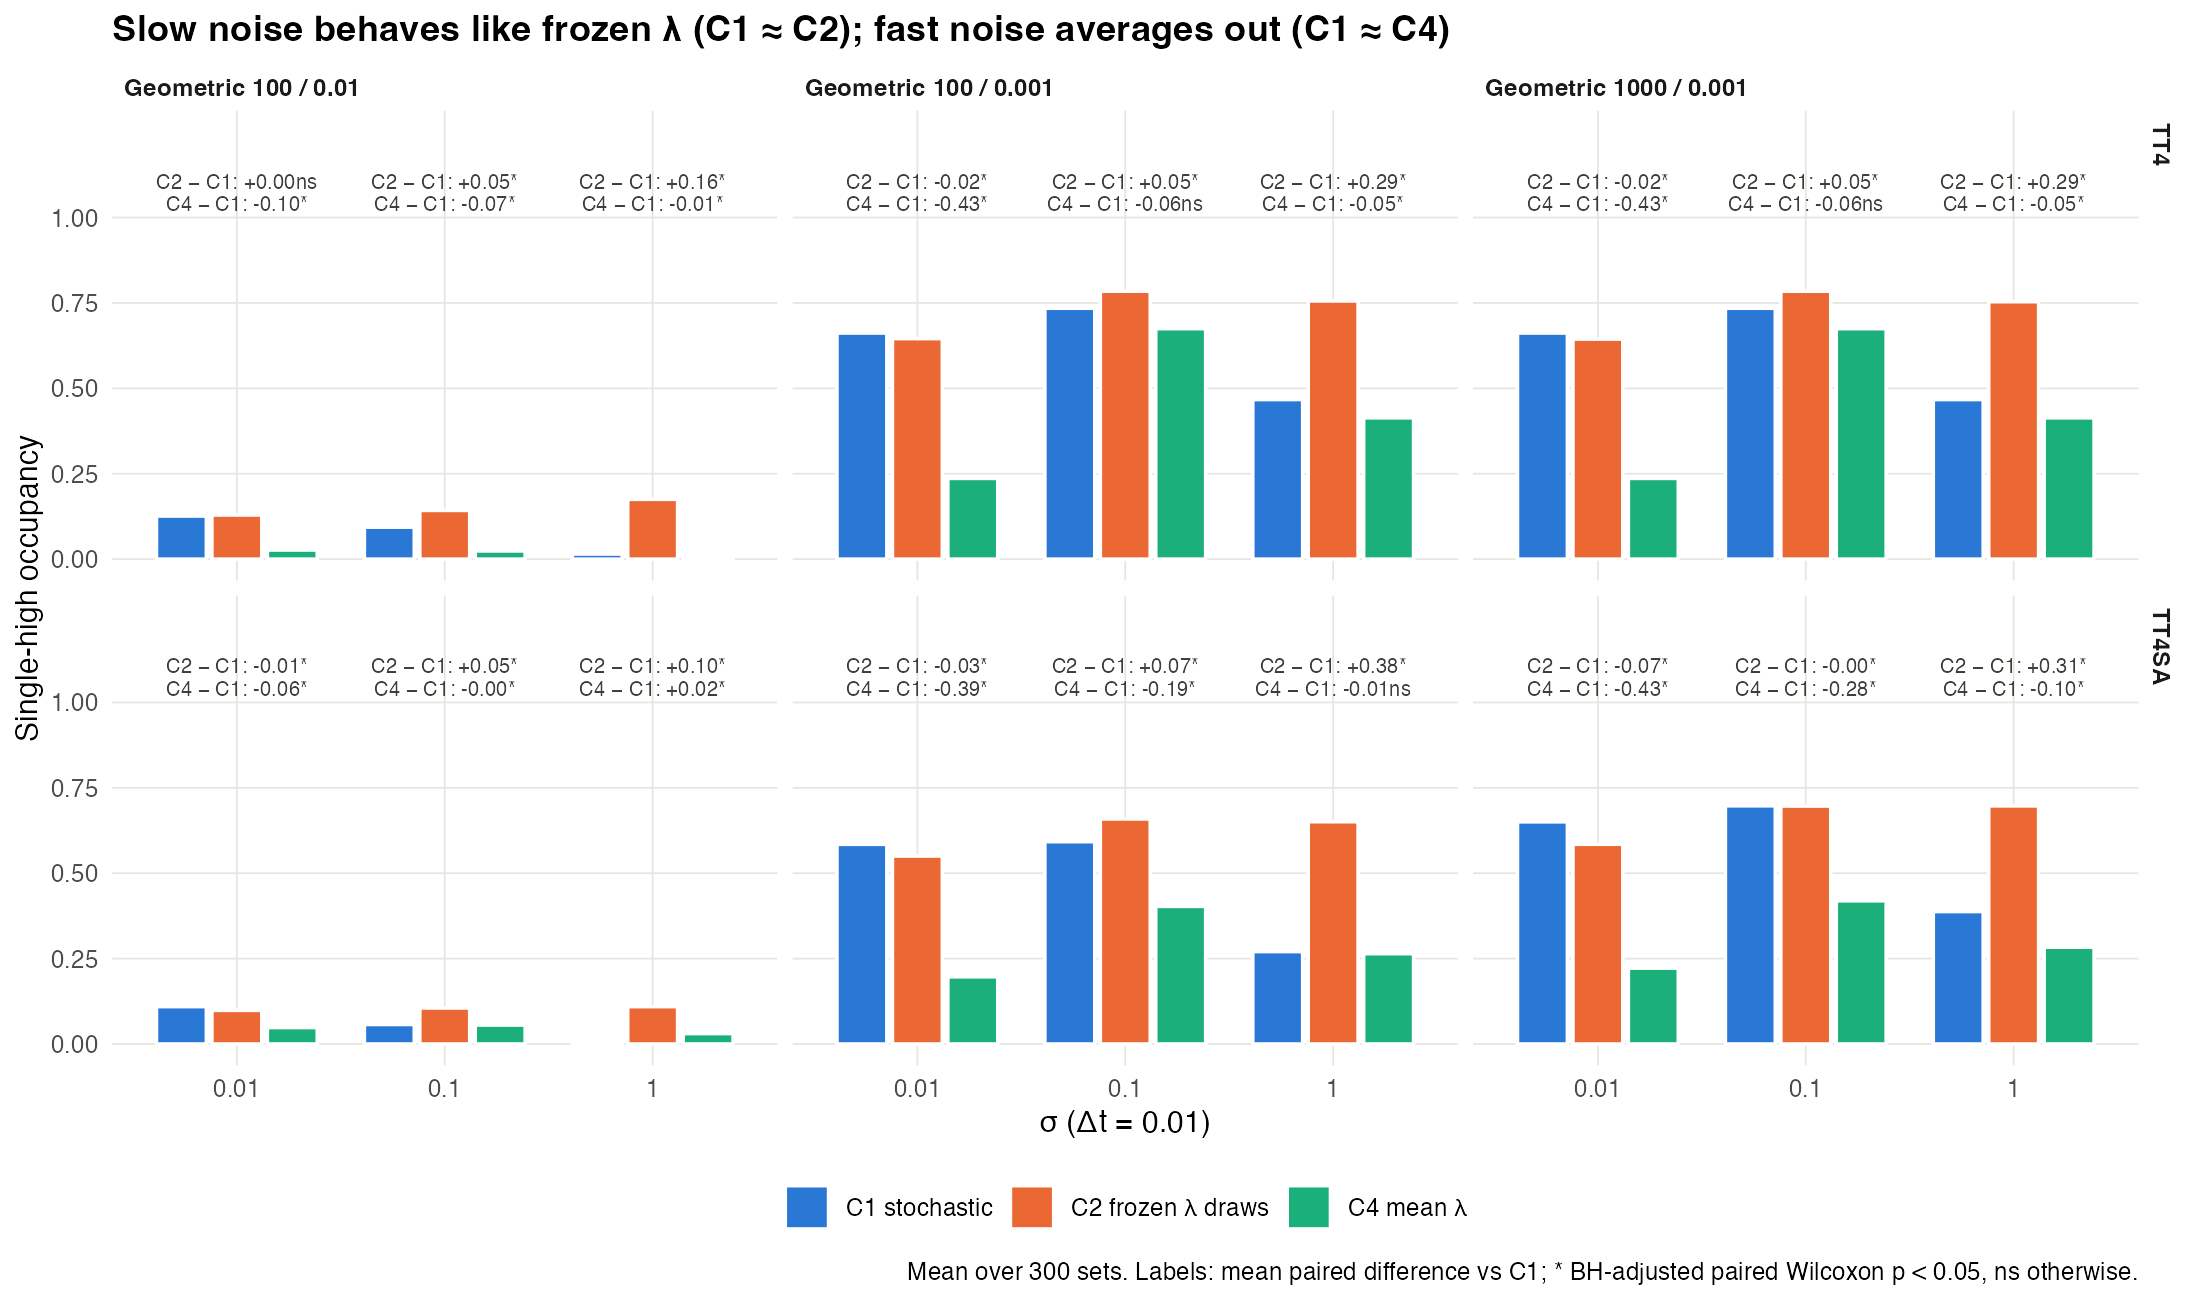
\includegraphics[width=\linewidth]{FigS_mult_controls.png}
    \caption{\textbf{Multiplicative noise: slow fluctuations act like frozen $\lambda$, fast fluctuations average out.} Single-high occupancy for TT4 and TT4SA under the geometric multiplicative rule, for the stochastic simulation (C1), frozen draws from the visited $\lambda$ distribution (C2) and the mean-$\lambda$ control (C4), at $dt = 0.01$. Columns, bounds on the fold-change (activation cap / inhibition floor). Labels, mean paired difference from C1; * BH-adjusted paired Wilcoxon $p < 0.05$. Pilot run, 100 parameter sets per stability class.}
    \label{fig:S_mult_controls}
\end{figure}

\begin{figure}
    \centering
    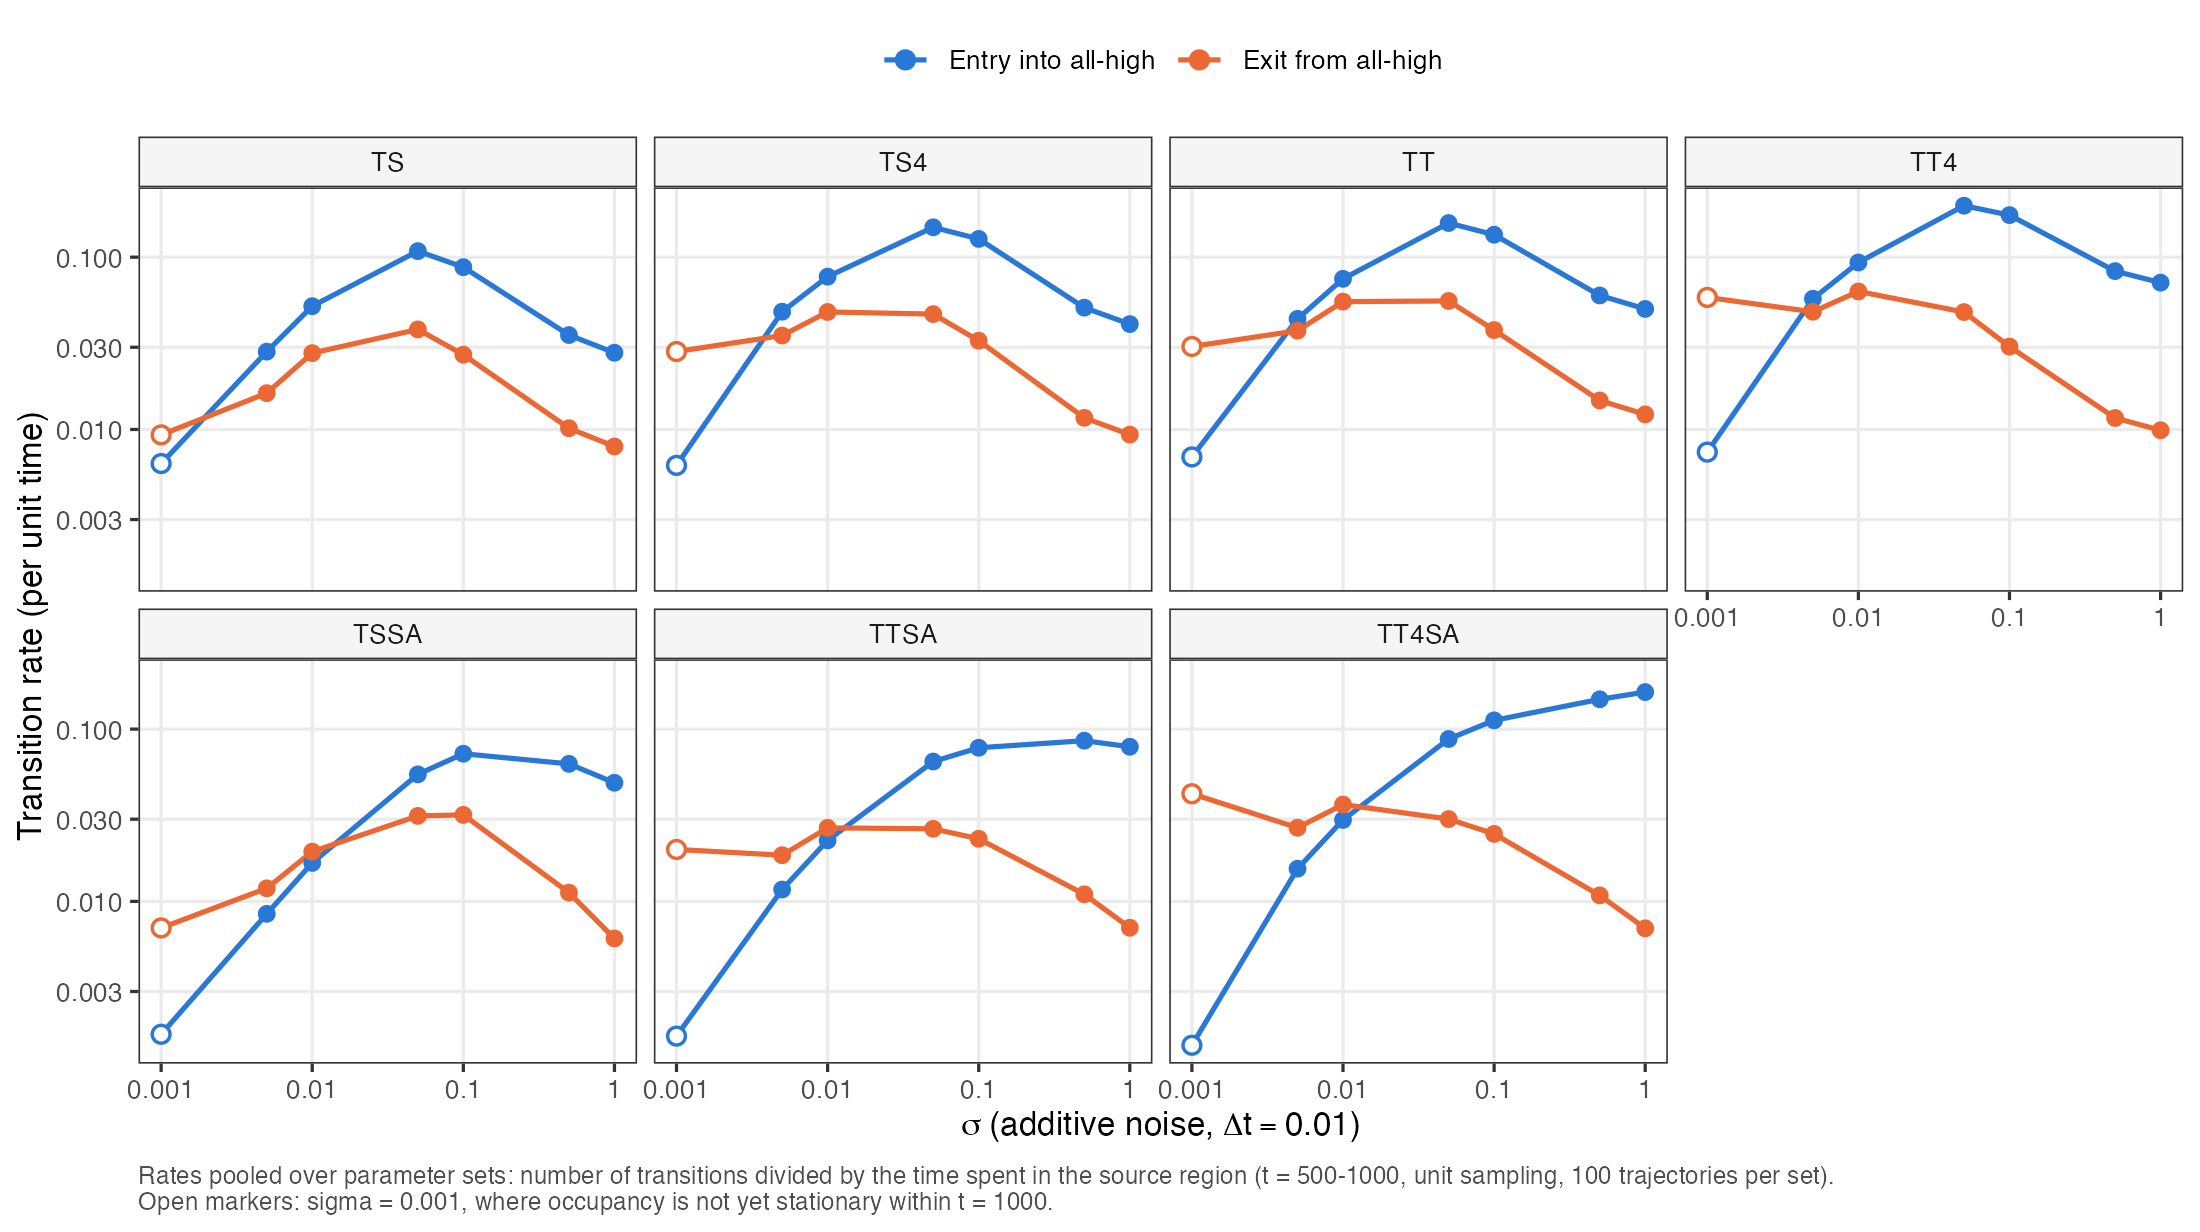
\includegraphics[width=\linewidth]{FigS_allhigh_rates.png}
    \caption{\textbf{Rates of entry into and exit from the all-high state under additive noise.} For each network and $\sigma$ ($dt = 0.01$), the entry rate is the number of transitions into all-high divided by the time spent outside it, and the exit rate is the number of transitions out of all-high divided by the time spent in it, pooled over parameter sets (100 trajectories each, unit sampling over $t = 500$--1000). Open markers, $\sigma = 0.001$, where occupancy is not yet stationary within $t = 1000$. At low noise the entry rate rises much faster than the exit rate; at high noise the exit rate falls faster than the entry rate.}
    \label{fig:S_rates}
\end{figure}


\begin{figure}
    \centering
    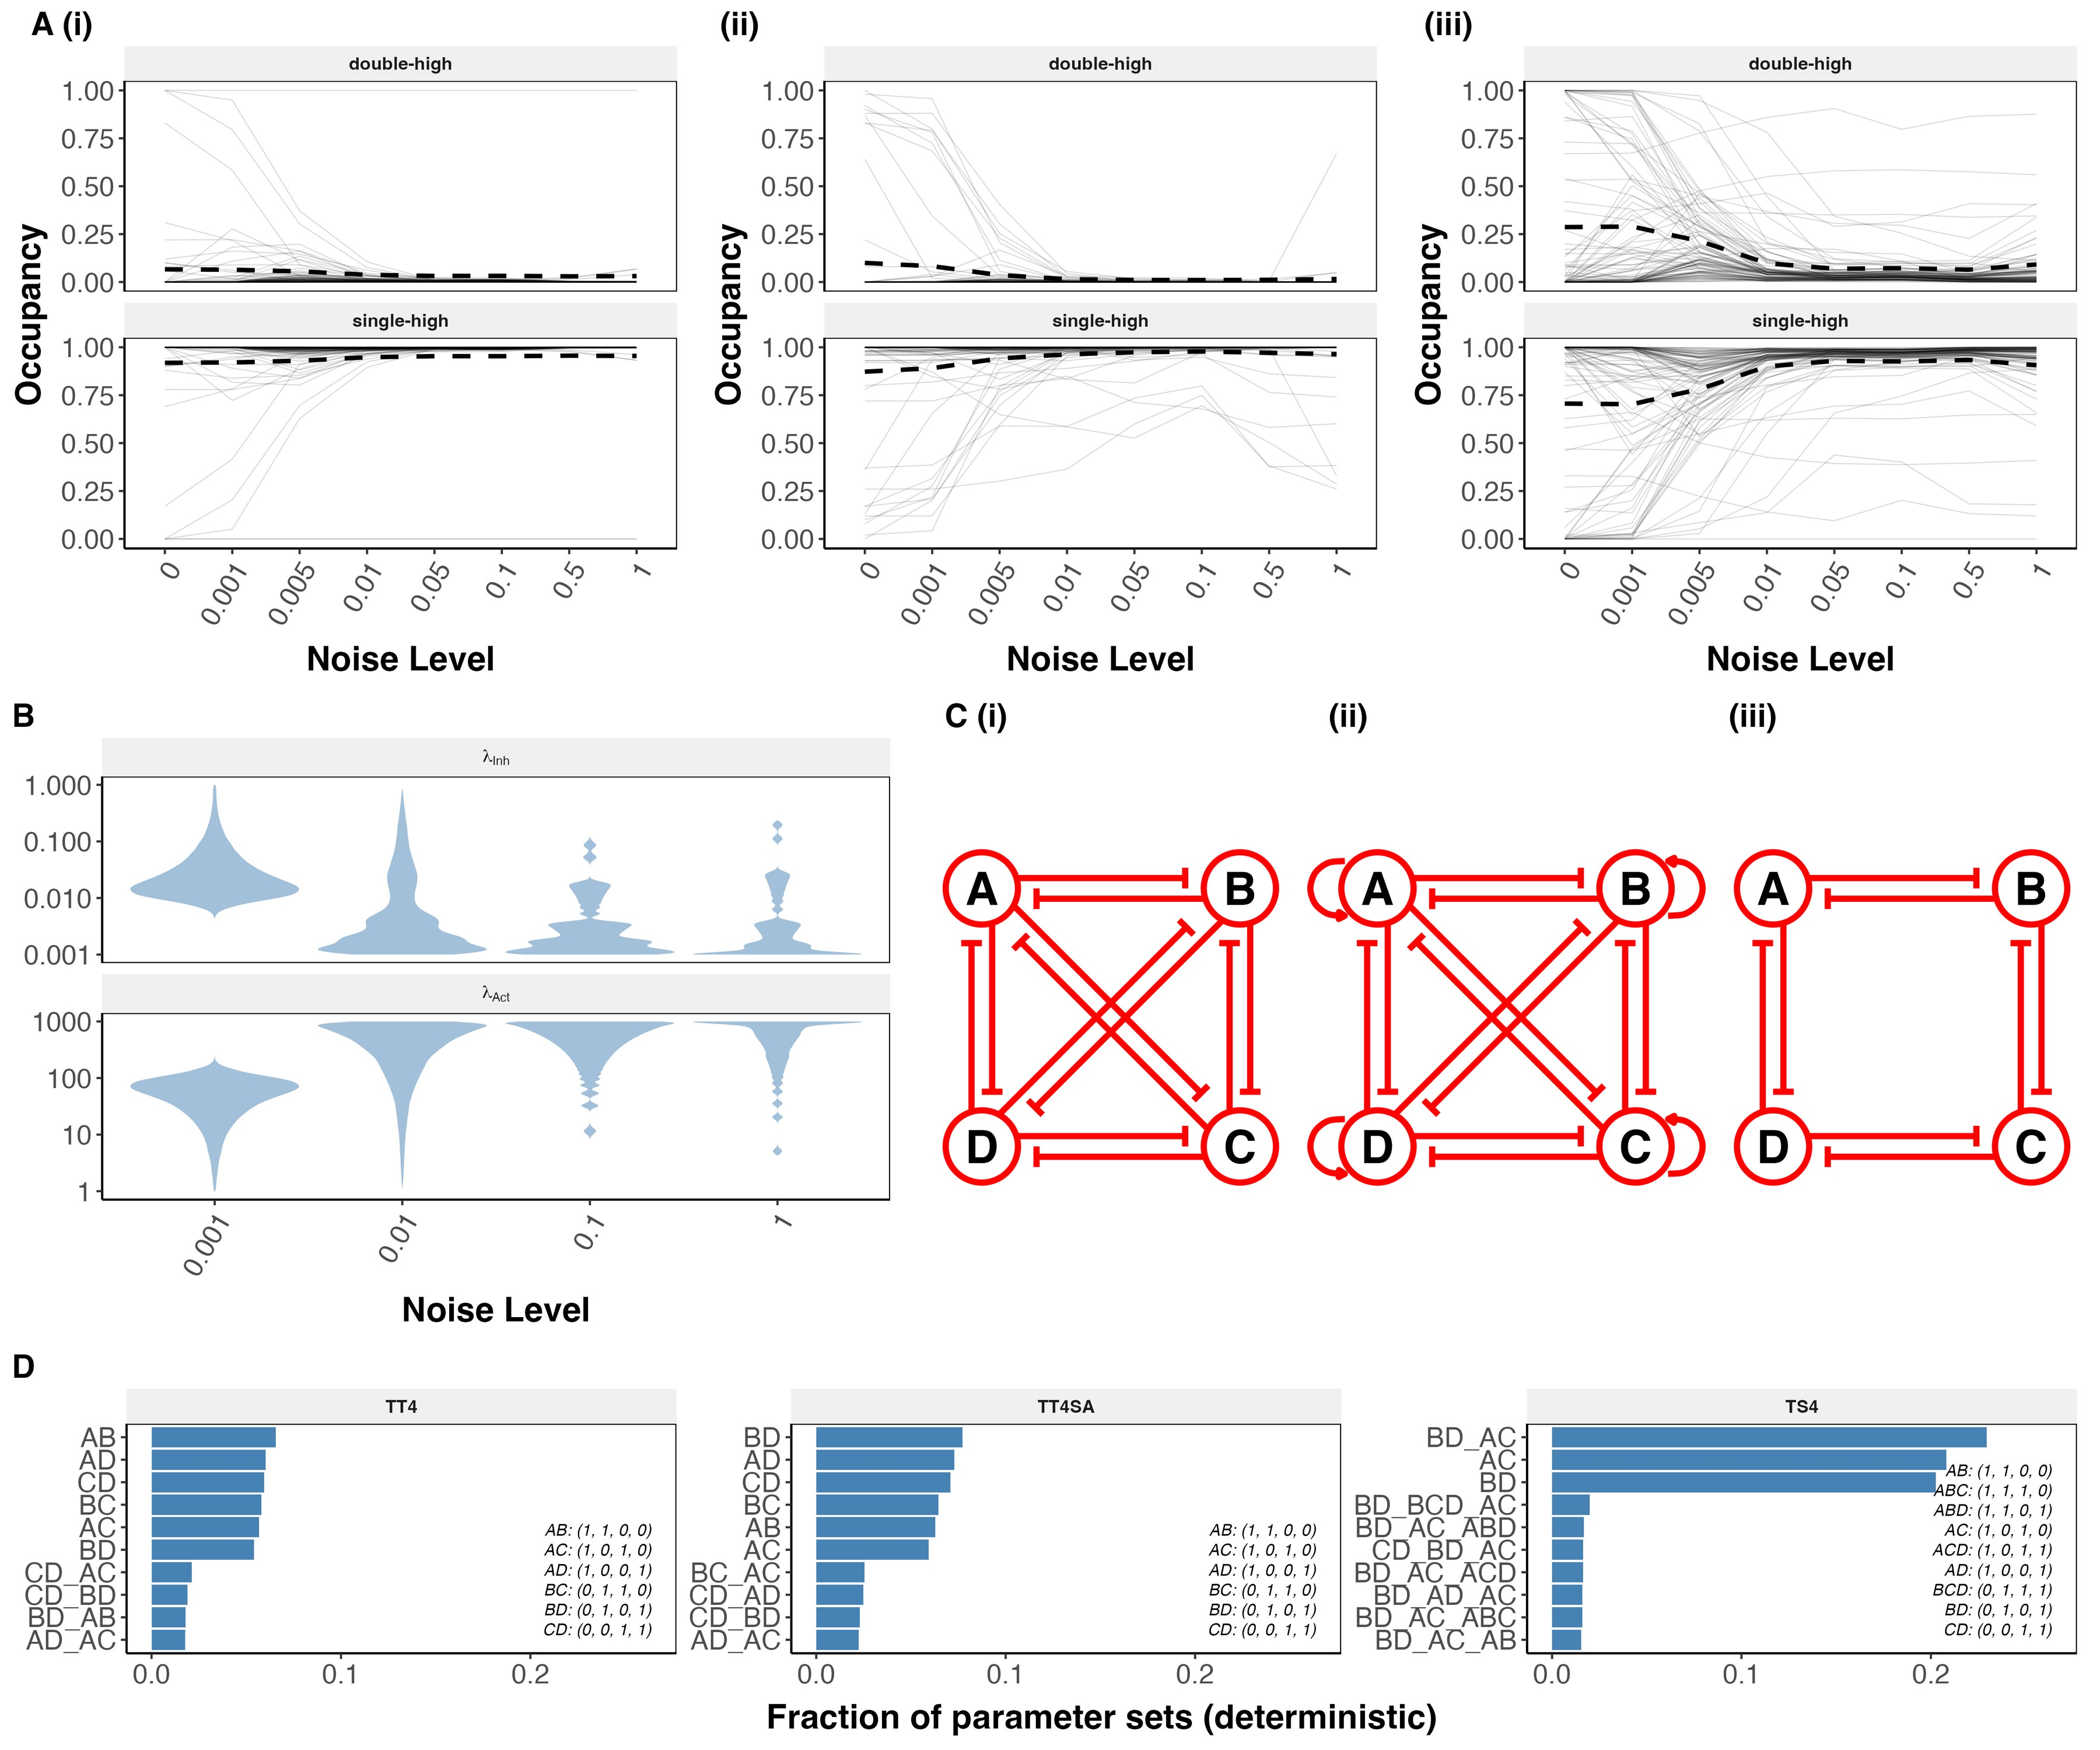
\includegraphics[width=0.8\linewidth]{Fig5S1.jpg}
    \caption{\textbf{(A)} Occupancy vs.\ noise level (as in Figure~\ref{fig:4}A, each showing a random sample of 100 parameter-set trajectories with the mean across the full population) for TS, TSSA, and TT; single-high and double-high state classes. For TS and TSSA, whose fully-active state is intrinsically ``all-high'' rather than a distinct ``double-high'' state, this facet is relabeled ``double-high'' for consistency with the other panels, but shows the same all-high data. \textbf{(B)} Distribution of $\lambda$ visited during the stochastic simulations (as in Figure~\ref{fig:3b}A) under multiplicative noise, inhibitory (TS, A$\to$B) and activating (TSSA, A$\to$A) edges, log scale. At $\sigma = 0.001$ the walk has not yet reached the bound within the analysis window; for $\sigma \geq 0.01$, $\lambda$ concentrates within about tenfold of maximal strength ($10^{-3}$ for inhibition, $10^{3}$ for activation). \textbf{(C)} Network topology diagrams for TT4, TT4SA, and TS4. \textbf{(D)} Deterministic attractor-combination frequency (as in Fig.\ 1C, but from the noise-simulation pipeline's zero-noise runs rather than RACIPE's own steady-state search) for TT4, TT4SA, and TS4.
}
    \label{fig:4S1}
\end{figure}

\begin{figure}
    \centering
    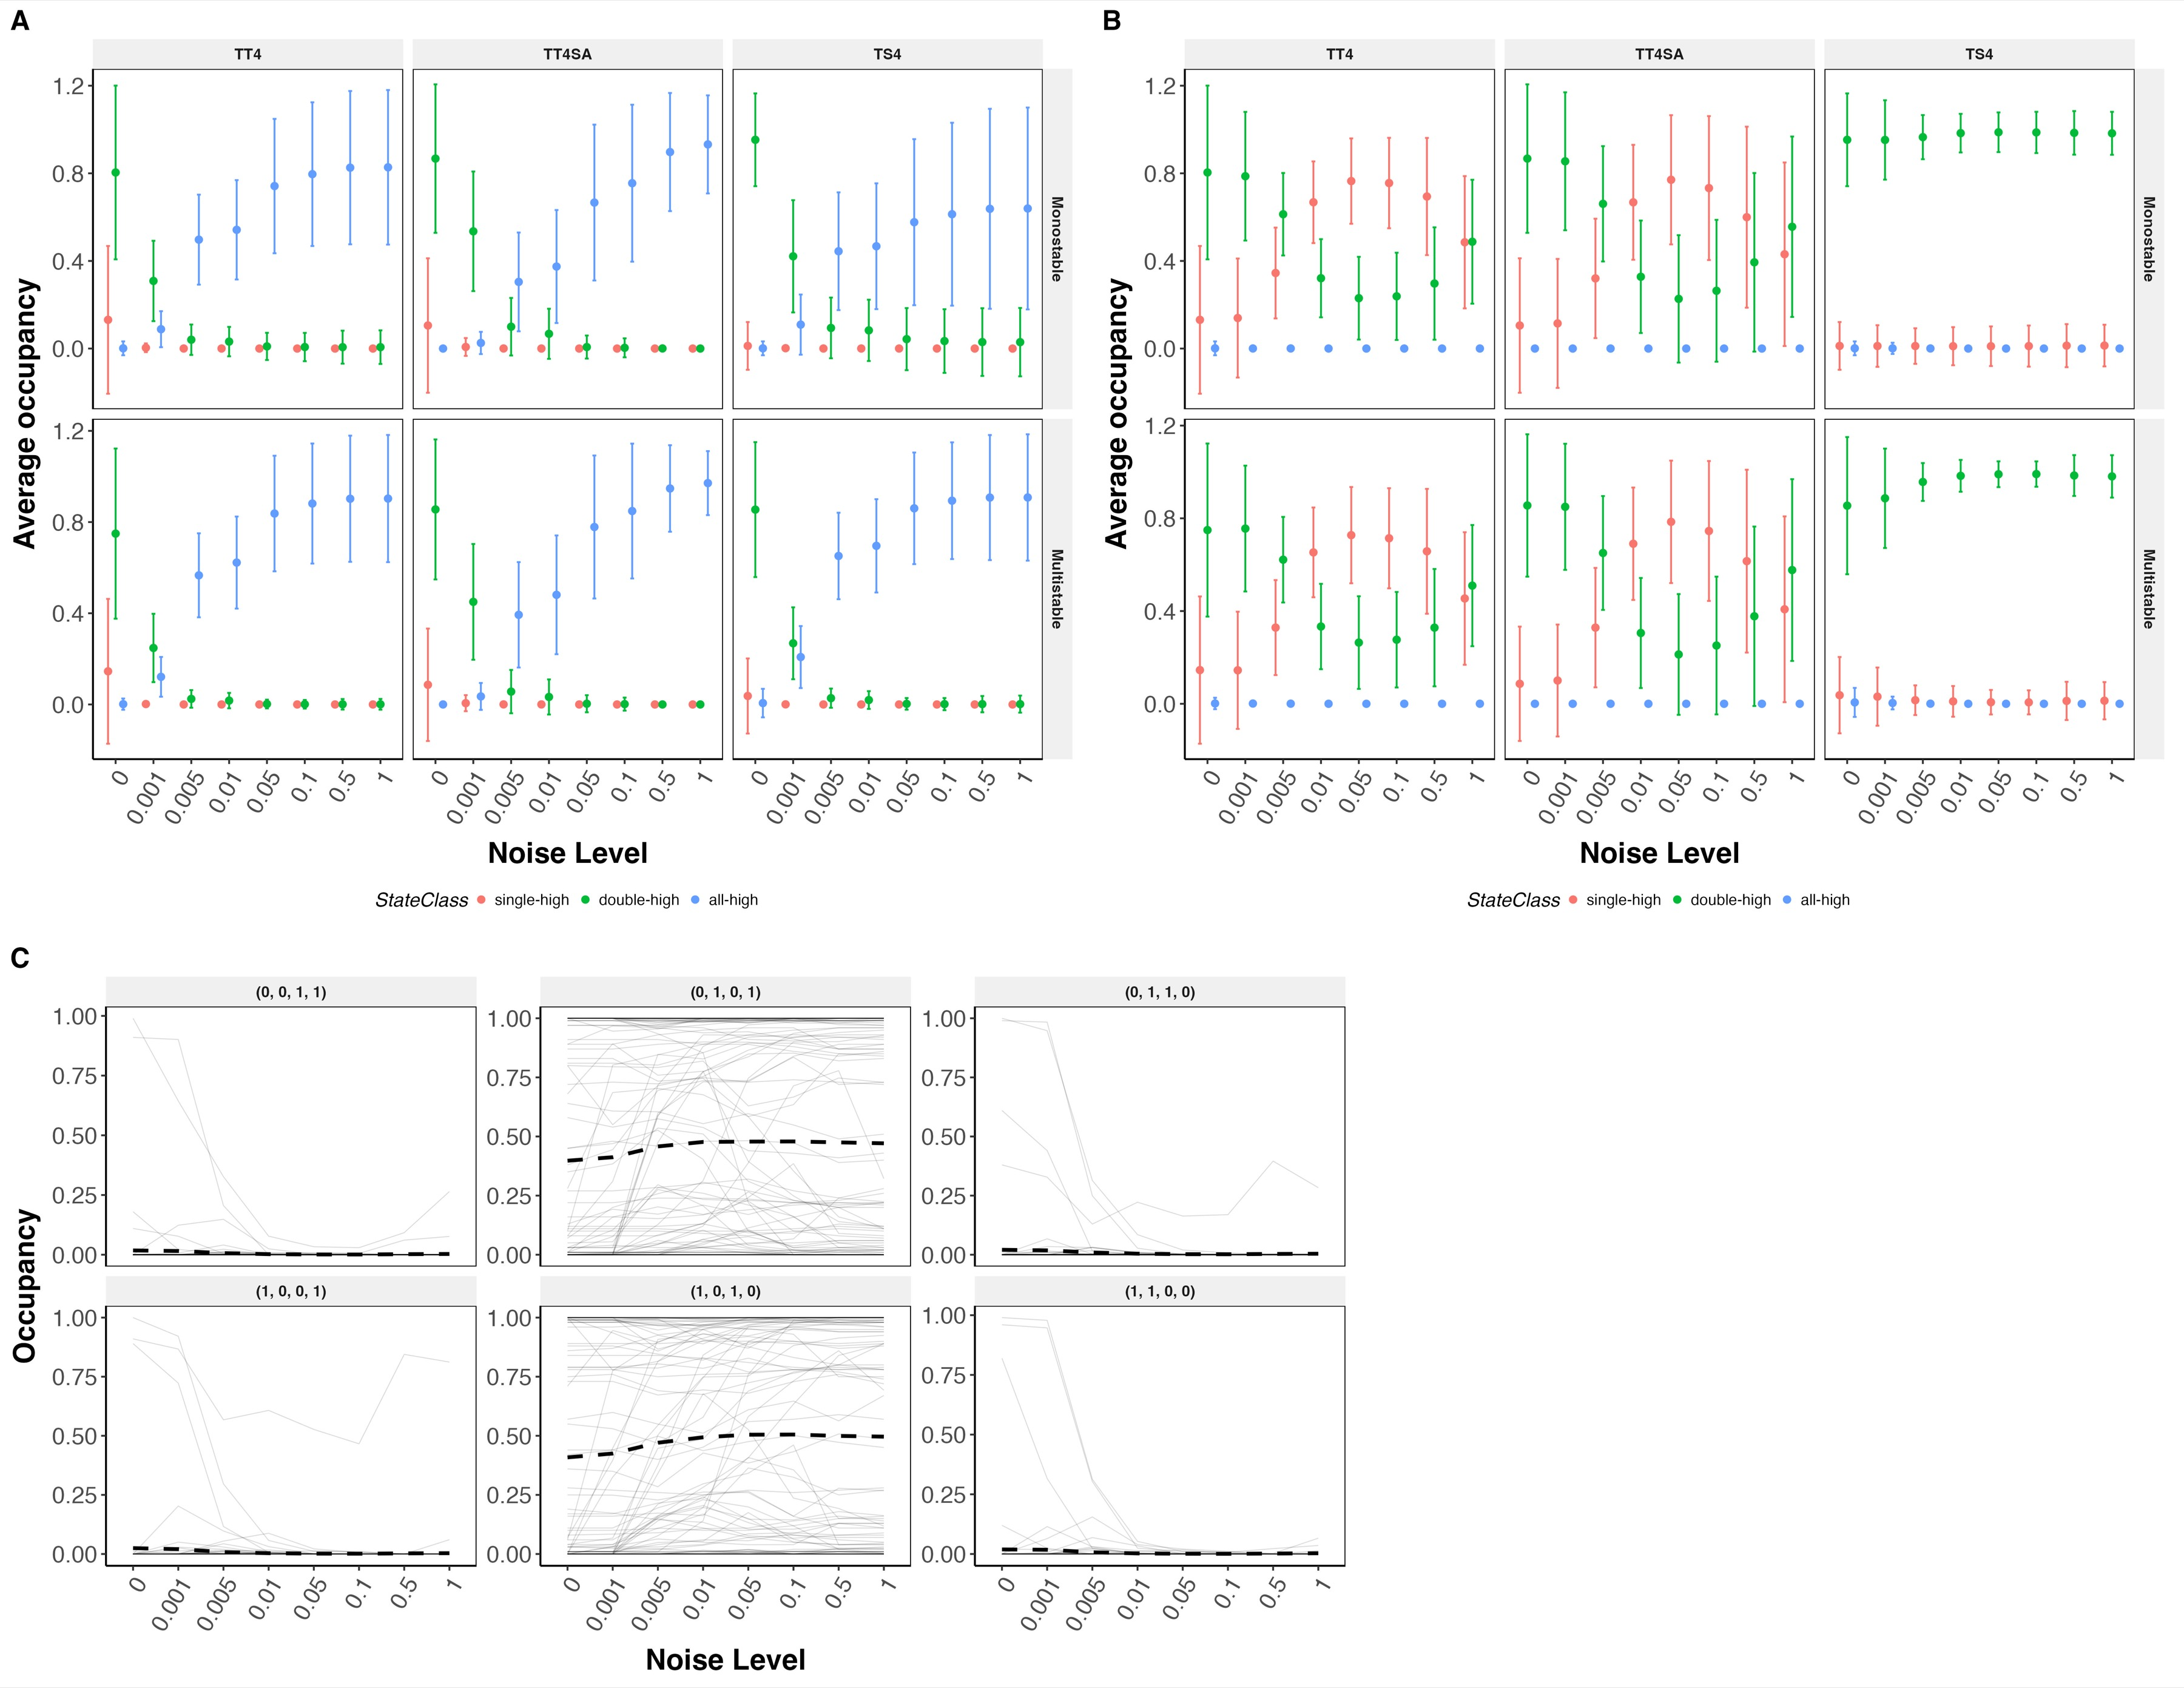
\includegraphics[width=0.8\linewidth]{Fig5S2.jpg}
    \caption{\textbf{(A, B)} Occupancy vs.\ noise level for TT4, TT4SA, and TS4; single-high, double-high, and all-high states, faceted by stability class, under Additive (A) and Multiplicative (B) noise. \textbf{(C)} State-wise occupancy vs.\ noise level for each of TS4's six double-high states individually (Multiplicative noise), showing that the same subset of states dominates at every noise level; grey lines show a random sample of 100 parameter-set trajectories, with the mean across the full parameter population shown separately. Mean $\pm$ SD over parameter sets; multiplicative noise follows the geometric rule ($\mu_{\min} = 10^{-3}$), $dt = 0.01$.
}
    \label{fig:4S2}
\end{figure}

\begin{figure}
    \centering
    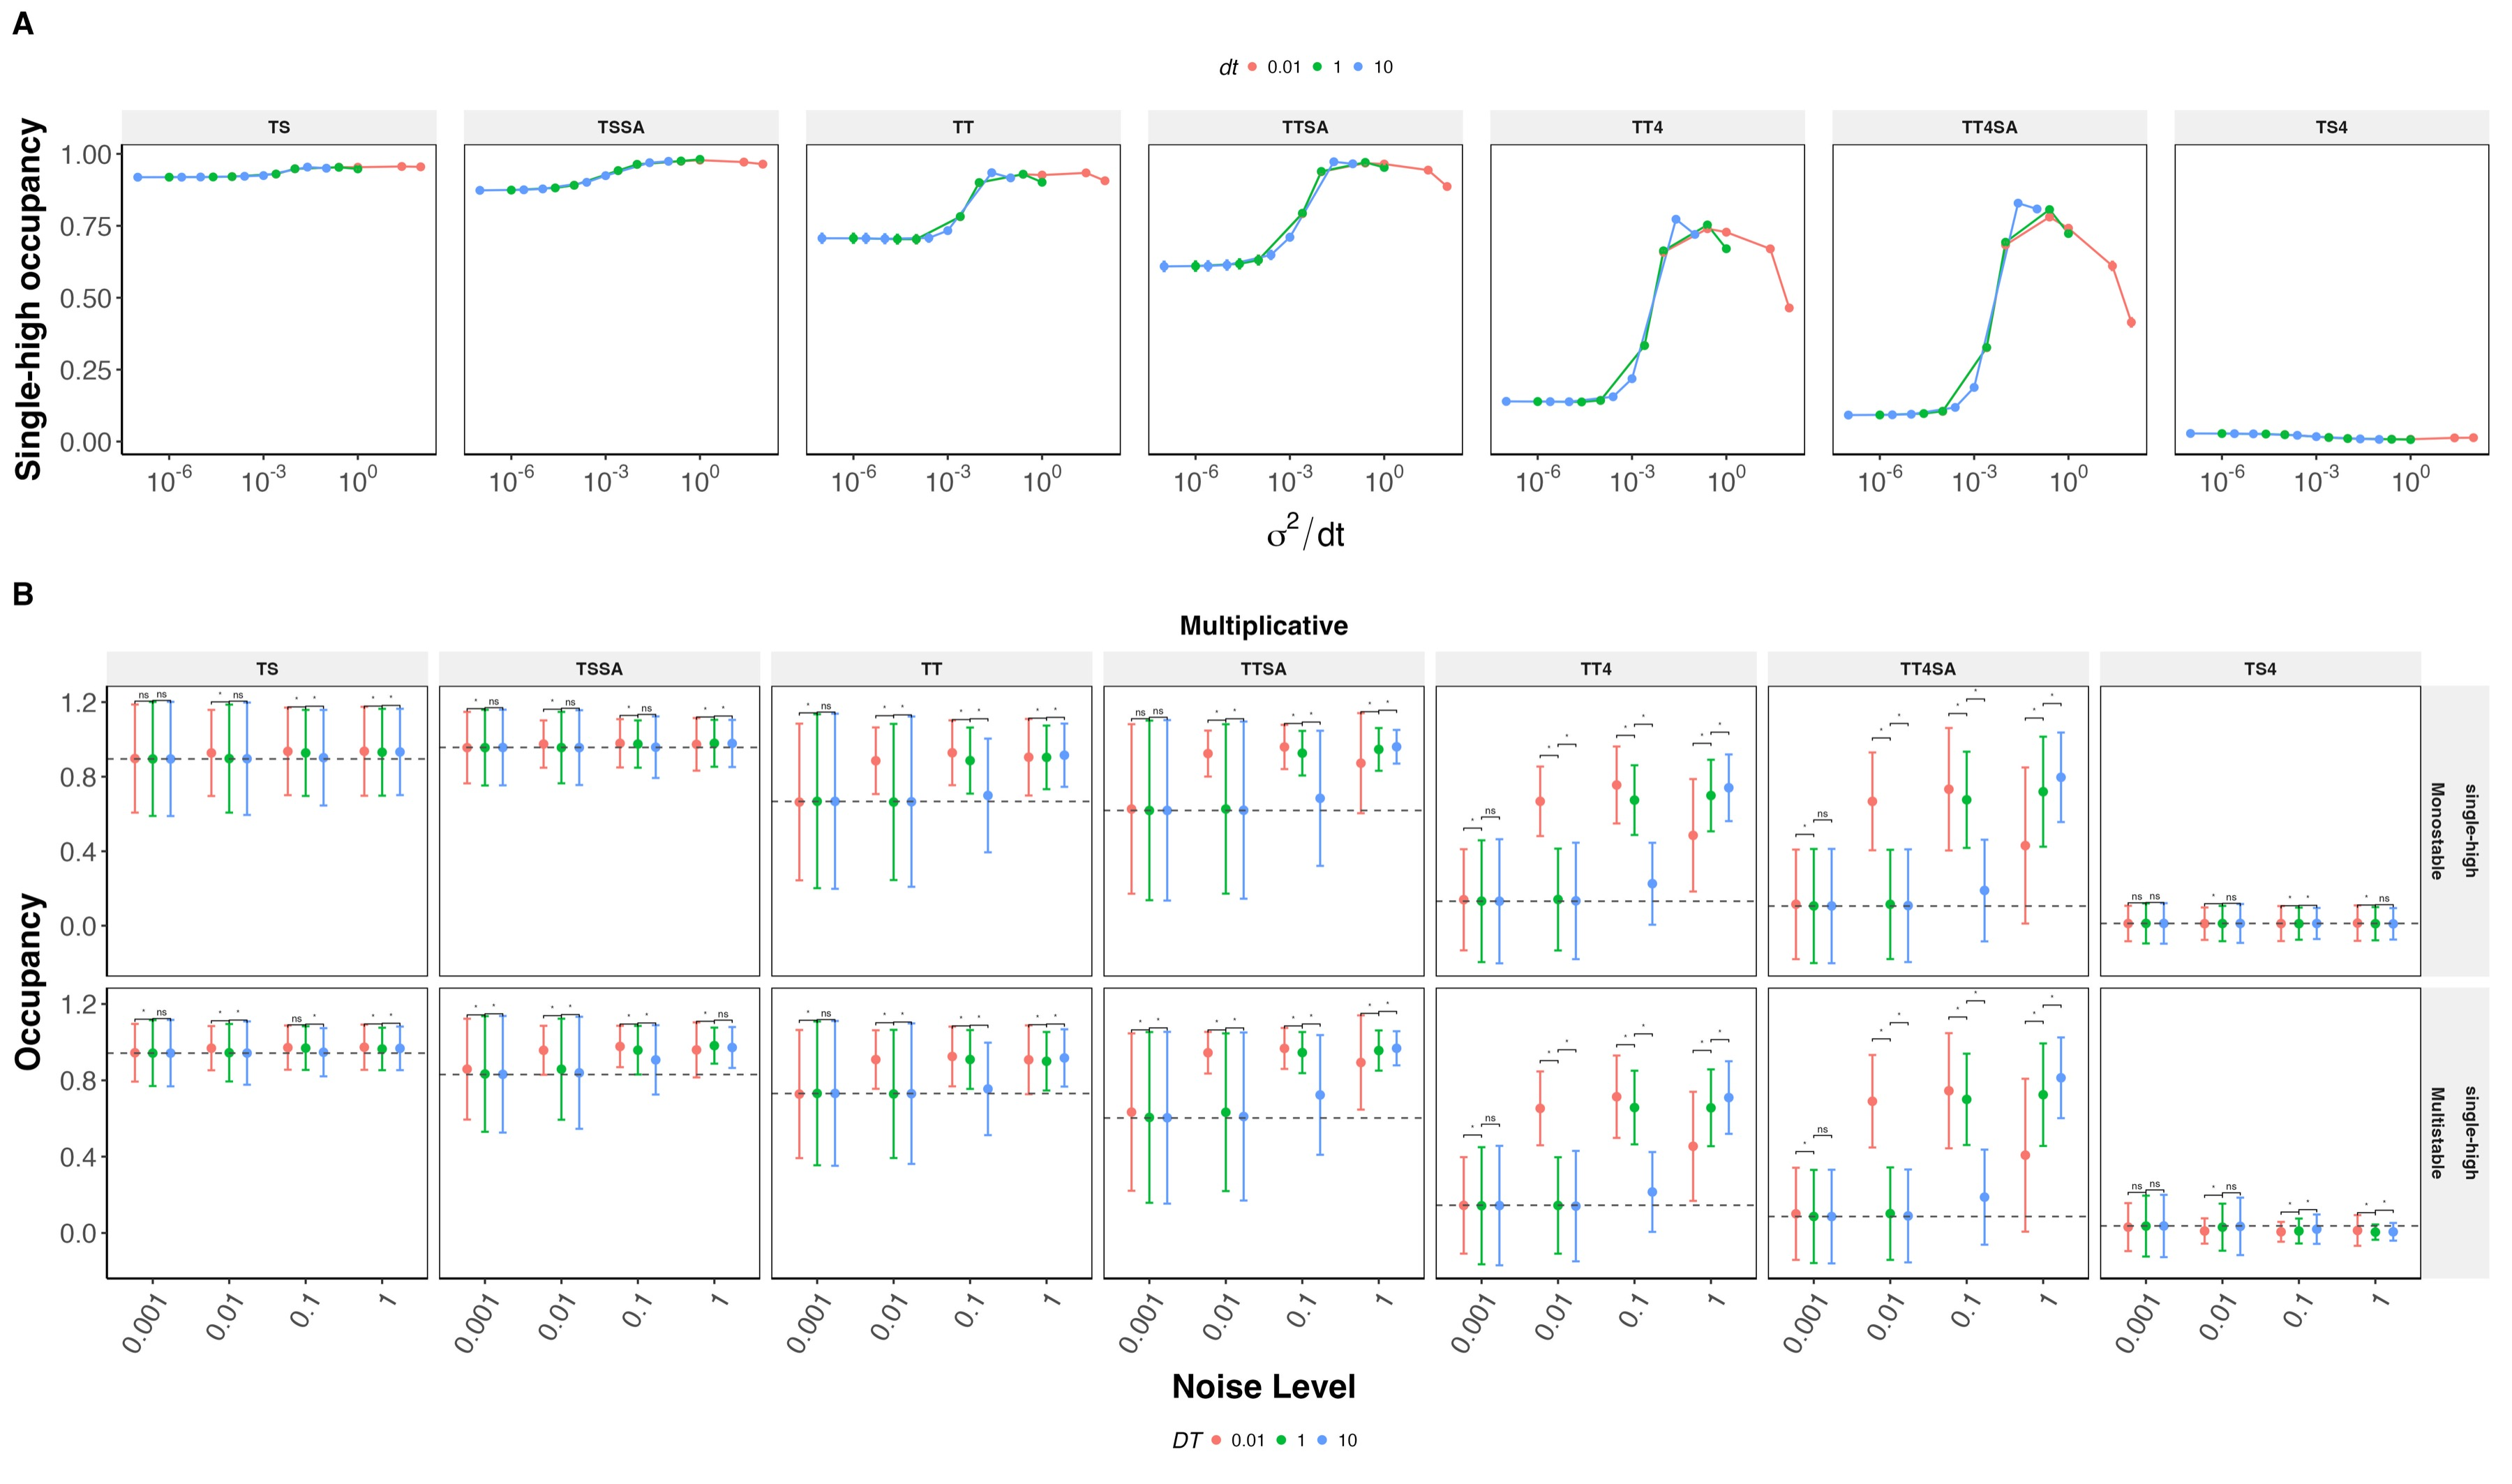
\includegraphics[width=0.8\linewidth]{Fig5S3.jpg}
    \caption{\textbf{Multiplicative noise depends on $\sigma$ and $dt$ only through $\sigma^2/dt$.} \textbf{(A)} Single-high occupancy of the stochastic simulation (mean $\pm$ 95\% CI over parameter sets) against $\sigma^2/dt$, for $dt = 0.01$, 1 and 10. Curves for different $dt$ overlap wherever they share $\sigma^2/dt$; they separate only at $\sigma \geq 0.5$, $dt = 0.01$, where $\lambda$ fluctuates faster than expression relaxes. \textbf{(B)} Single-high occupancy against $\sigma$ for each $dt$, by stability class (mean $\pm$ SD over parameter sets; paired Wilcoxon tests between adjacent $dt$; dashed line, noise-free value). Geometric rule, $\mu_{\min} = 10^{-3}$.}
    \label{fig:4S3}
\end{figure}

\begin{figure}
    \centering
    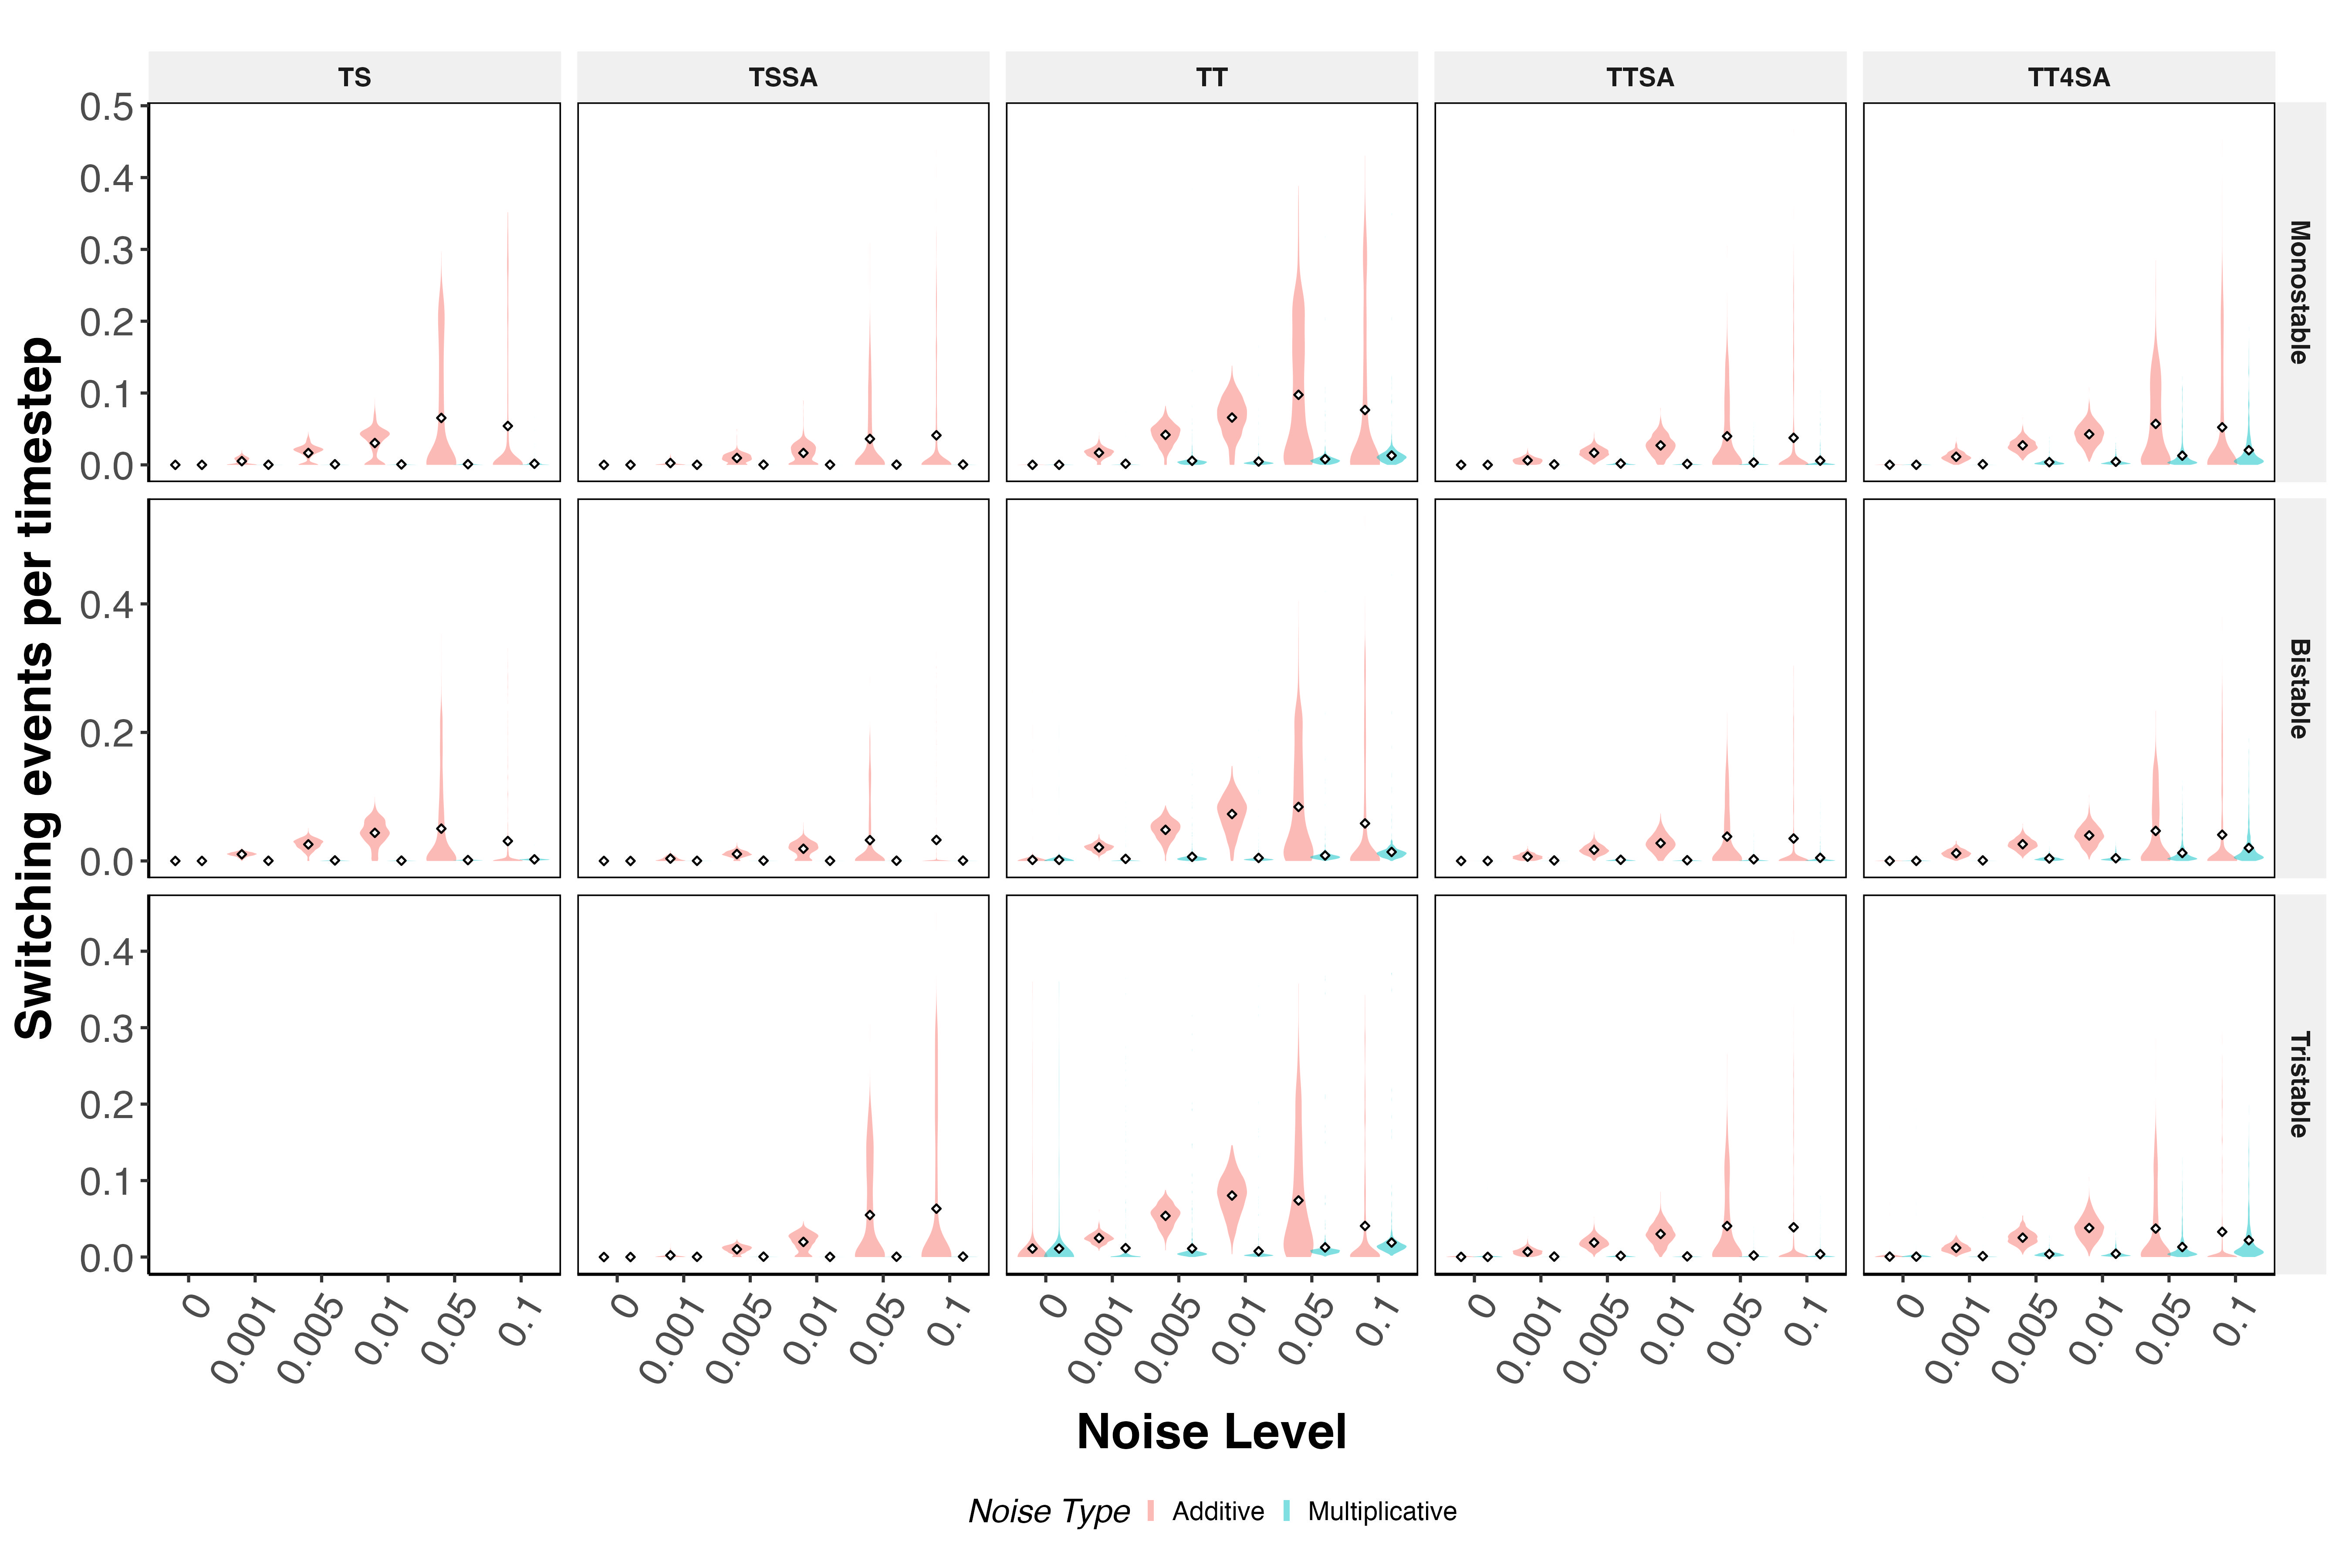
\includegraphics[width=0.8\linewidth]{Fig6S1.jpg}
    \caption{\textbf{Switching-event rates generalize across networks and stability classes.}
    Distribution of switching-event counts per timestep by noise level (Additive vs.\ Multiplicative), for TS, TSSA, TT, TTSA, and TT4SA, faceted by network (columns) and deterministic stability class (rows). TS has no Tristable class (a 2-node network cannot support 3+ distinct stable states), so that facet is empty. Multiplicative noise follows the geometric rule ($\mu_{\min} = 10^{-3}$), $dt = 0.01$.
}
    \label{fig:6S1}
\end{figure}

\begin{figure}
    \centering
    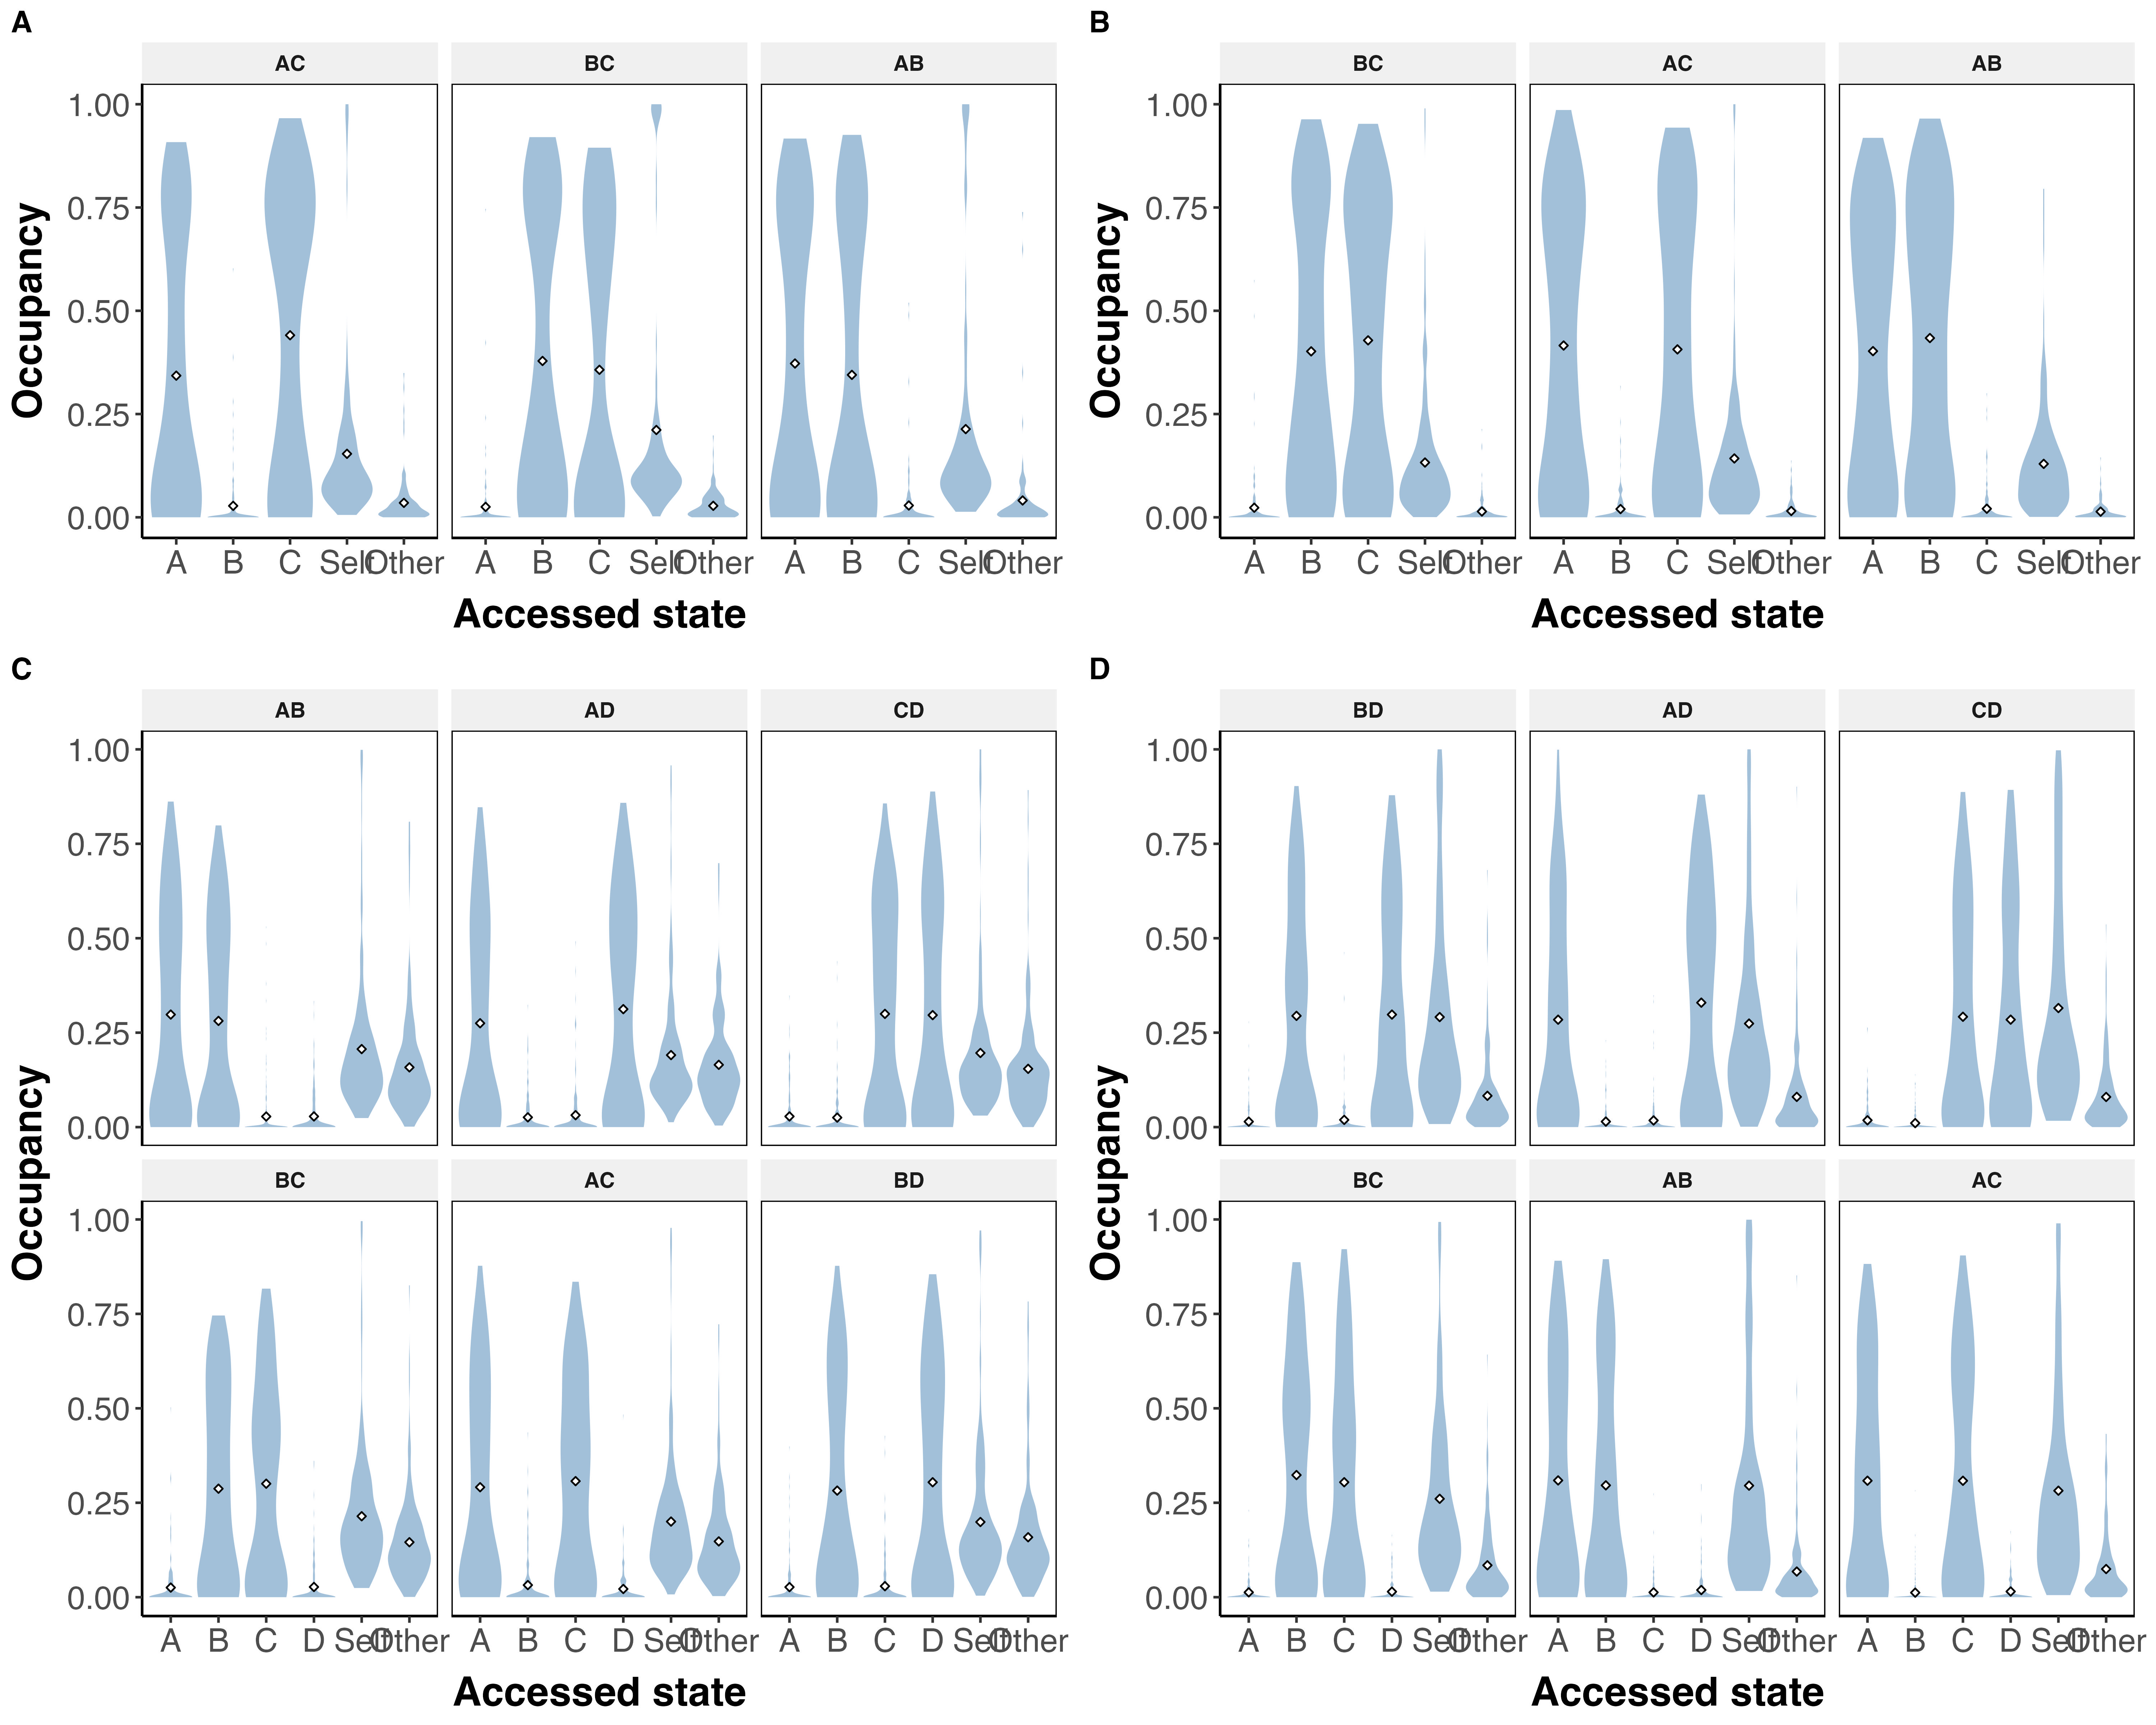
\includegraphics[width=0.8\linewidth]{Fig6S2.jpg}
    \caption{\textbf{Nearest-fate resolution holds for every individual double-high attractor.}
    Per-parameter occupancy distribution at noise = 0.01, shown separately for each monostable double-high attractor combination (one facet per combination), for \textbf{(A)} TT, \textbf{(B)} TTSA, \textbf{(C)} TT4, and \textbf{(D)} TT4SA. Multiplicative noise (geometric rule, $\mu_{\min} = 10^{-3}$), $dt = 0.01$.
}
    \label{fig:6S2}
\end{figure}

\begin{figure}
    \centering
    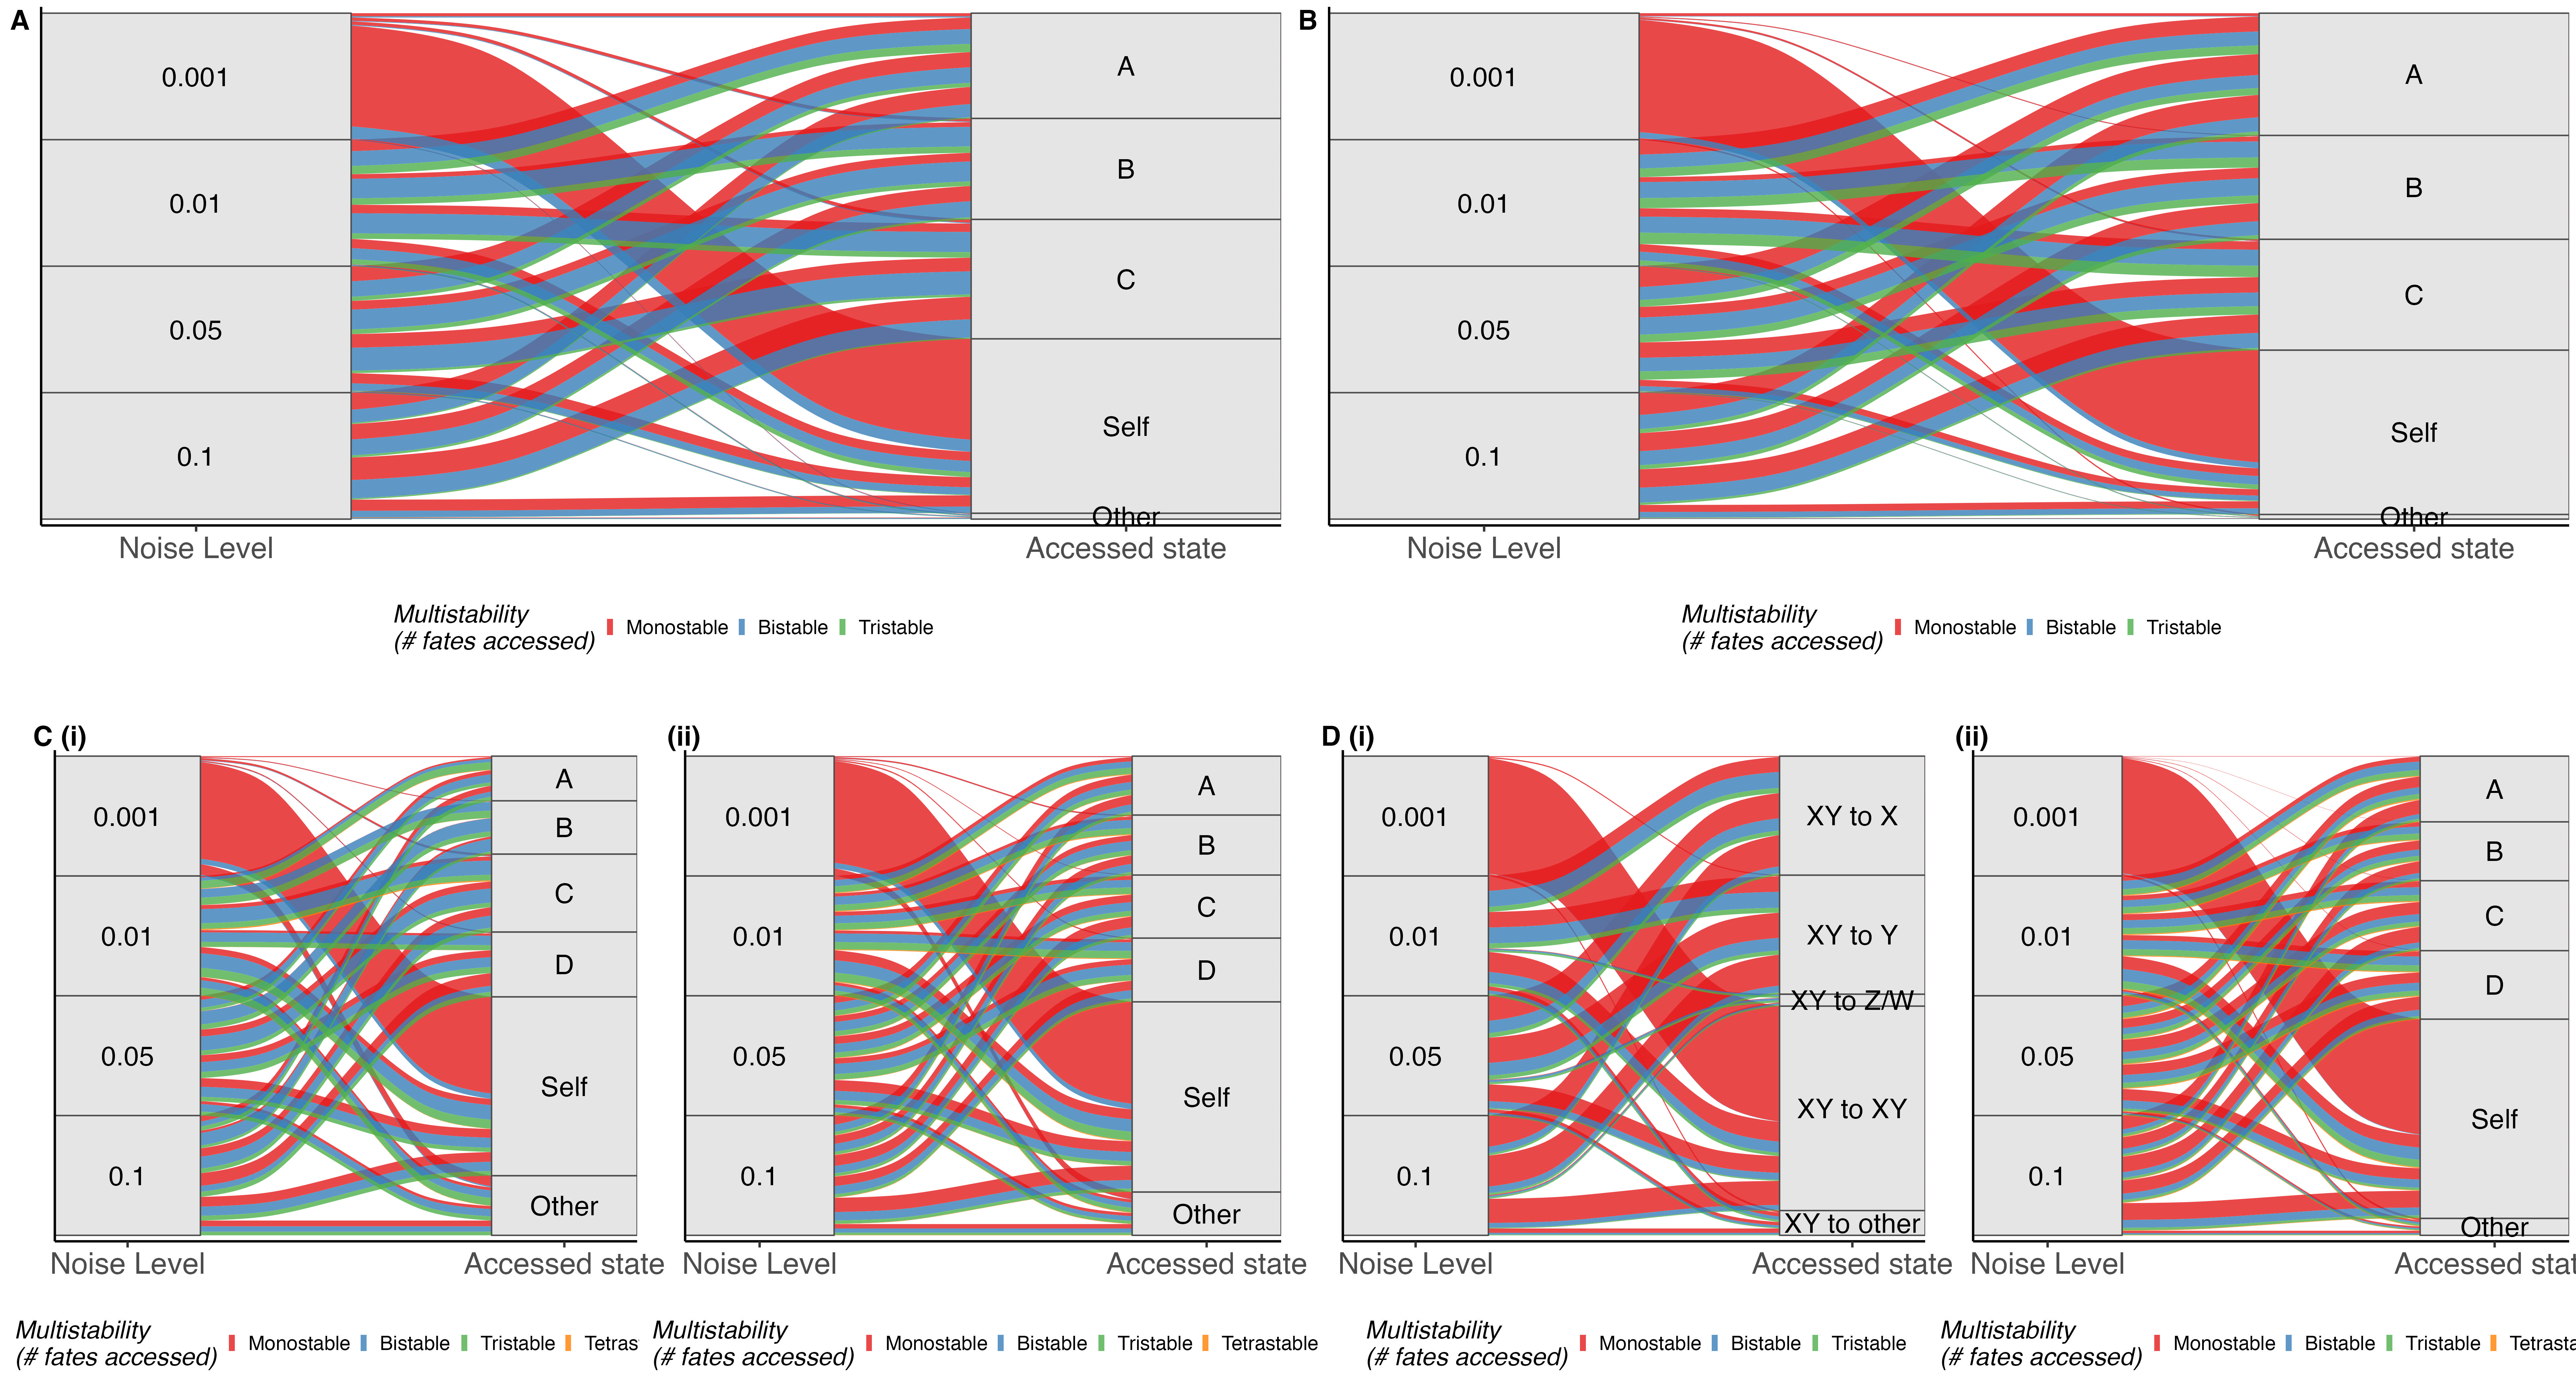
\includegraphics[width=\linewidth]{Fig6S3.jpg}
    \caption{\textbf{Noise-level $\to$ fate alluvials for the bistable double-high classes.}
    Noise-level $\to$ outcome alluvial (as in Figure~\ref{fig:6}E), colored by the multistability classification from Figure~\ref{fig:6}C, for the bistable double-high stability class: \textbf{(A)} TT and \textbf{(B)} TTSA, non-mirror only (mirror bistability is structurally impossible for these 3-node networks). \textbf{(C)} TT4, mirror \textbf{(i)} and non-mirror \textbf{(ii)} shown separately. \textbf{(D)} TT4SA, monostable double-high class \textbf{(i)} (as in Figure~\ref{fig:6}E, for this network) and bistable double-high class \textbf{(ii)}, with mirror and non-mirror populations pooled (TT4SA's mirror-bistable population alone is too sparse, 14 parameter sets, to interpret on its own). Multiplicative noise (geometric rule, $\mu_{\min} = 10^{-3}$), $dt = 0.01$.
}
    \label{fig:6S3}
\end{figure}

\begin{figure}
    \centering
    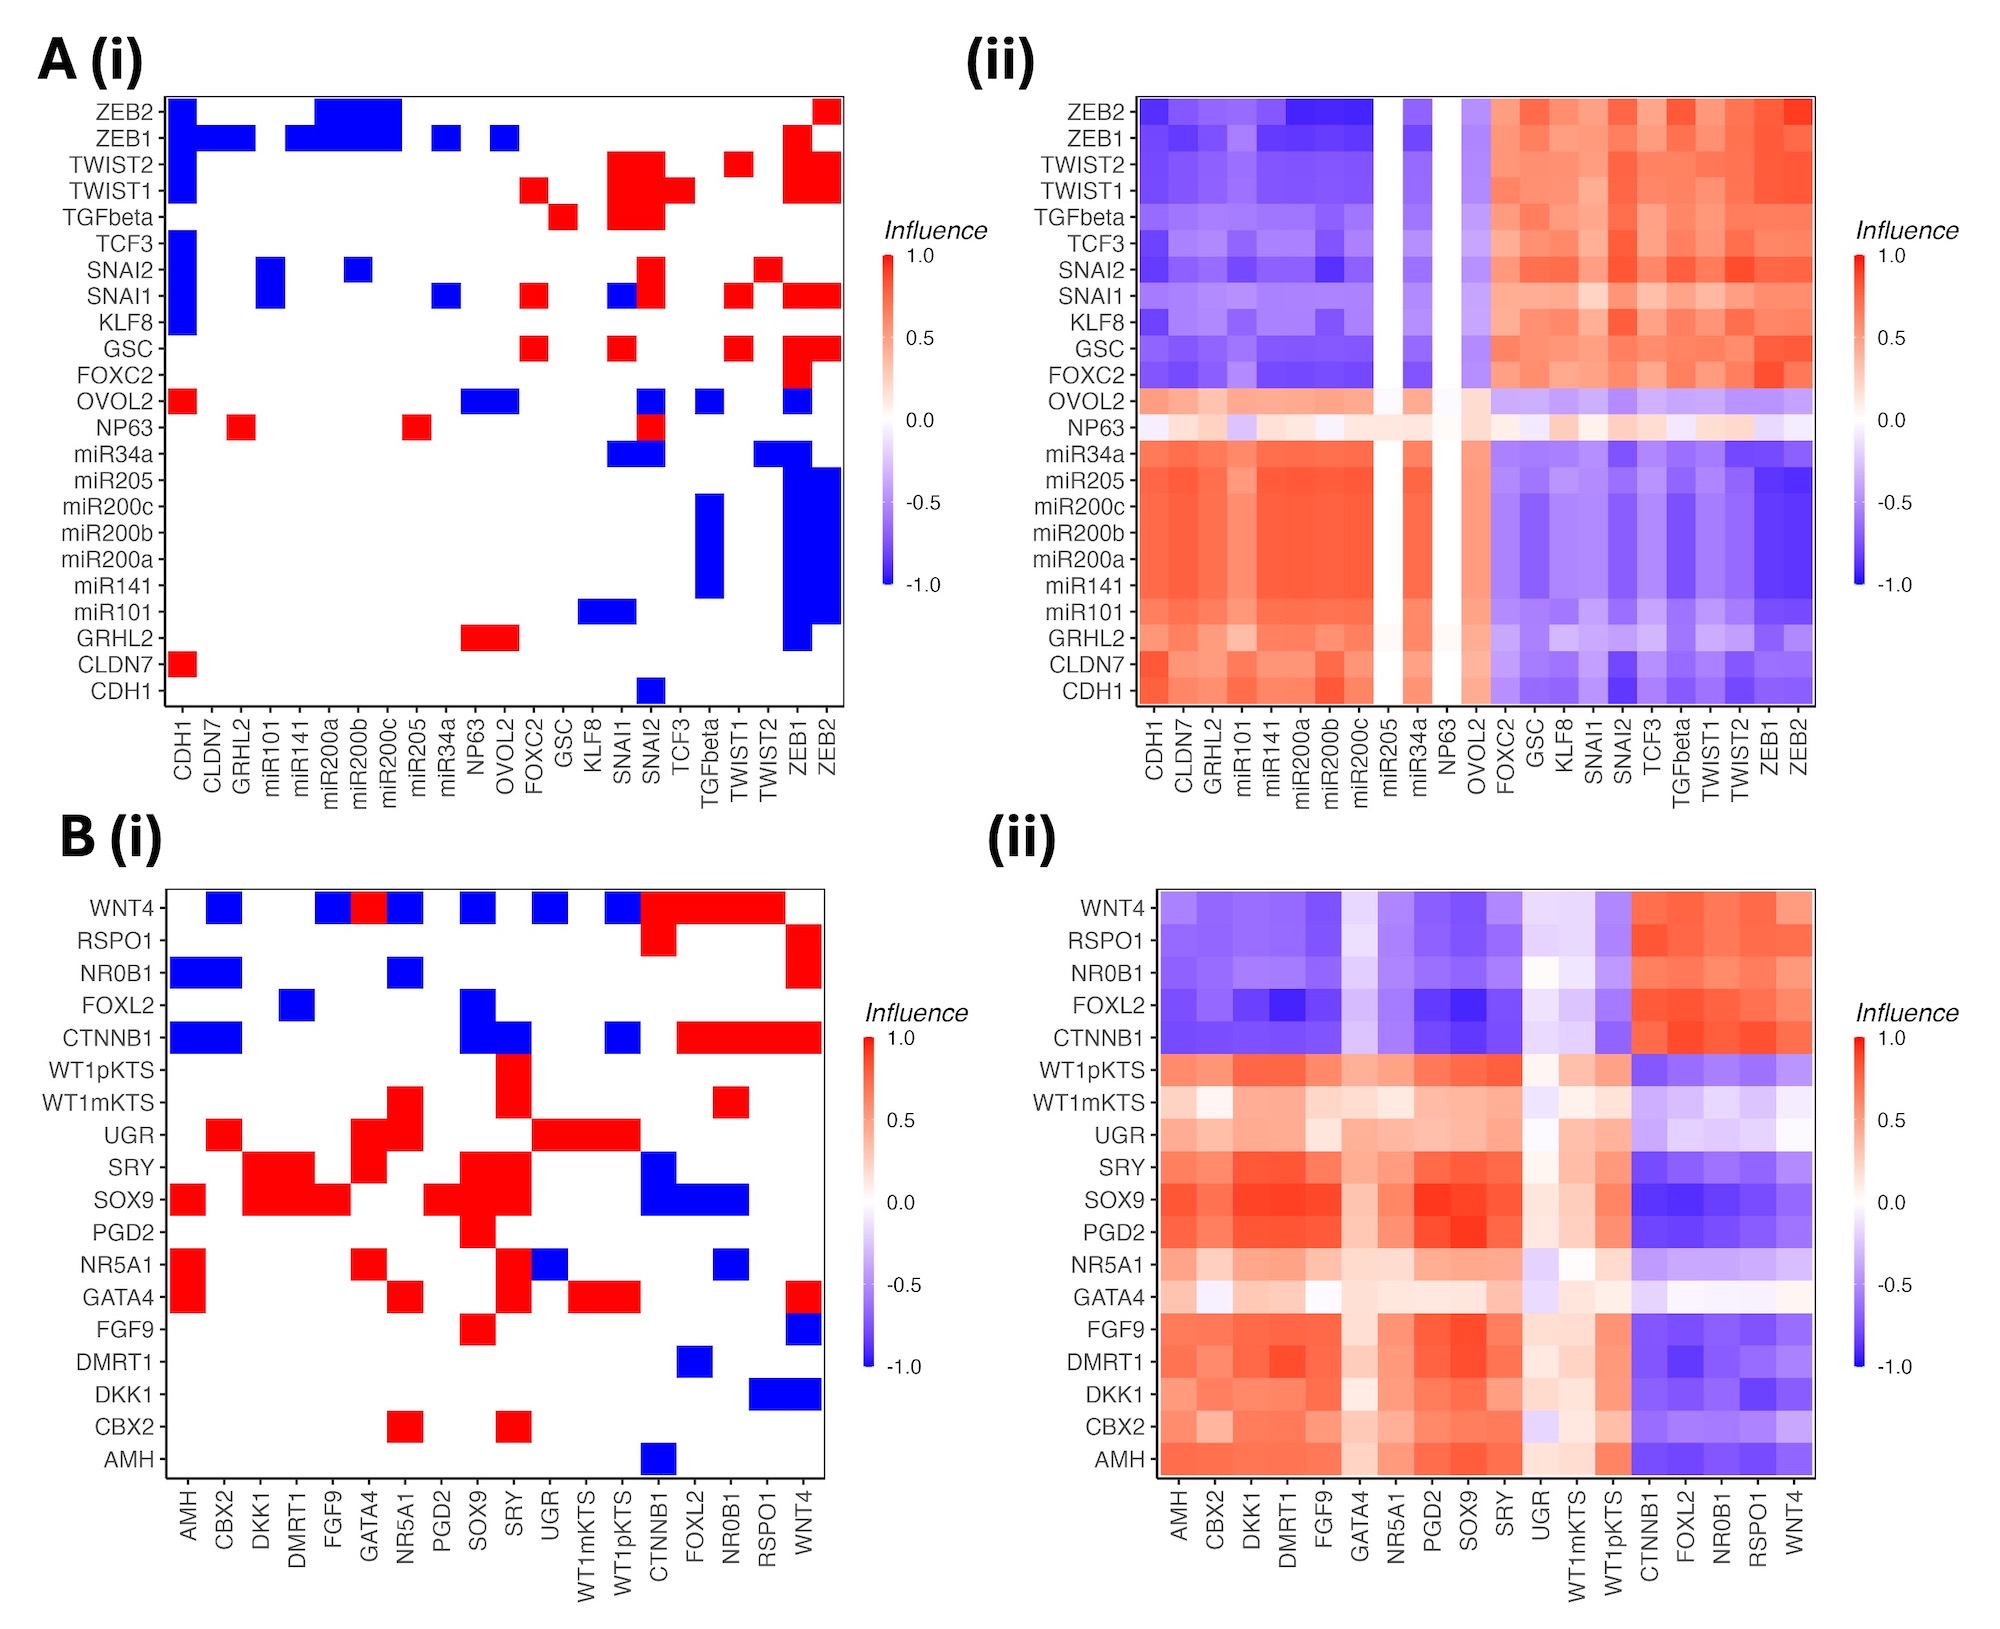
\includegraphics[width=0.8\linewidth]{Fig7S1.jpg}
    \caption{\textbf{Adjacency and influence matrices for the EMT and Gonadal networks.}
    A) EMT network (23 nodes). (i) Direct adjacency matrix showing the signed regulatory
    interactions between node pairs: red indicates activation ($+1$), blue indicates
    inhibition ($-1$), and white indicates no edge. Nodes are ordered by team membership,
    with the epithelial team in the lower-left block and the mesenchymal team in the
    upper-right block. (ii) Influence matrix computed as described in the Methods, showing
    the net cumulative effect between each pair of nodes across all path lengths up to
    $l_{\mathrm{max}} = 10$. Positive (red) values indicate net co-regulation; negative
    (blue) values indicate net counter-regulation. The block structure of the influence
    matrix confirms the two-team organisation of the network.
    B) Gonadal network (19 nodes), displayed in the same format as A, with the
    Sertoli-fate team and the Granulosa-fate team forming the two blocks.}
    \label{fig:7S1}
\end{figure}

\begin{figure}
    \centering
    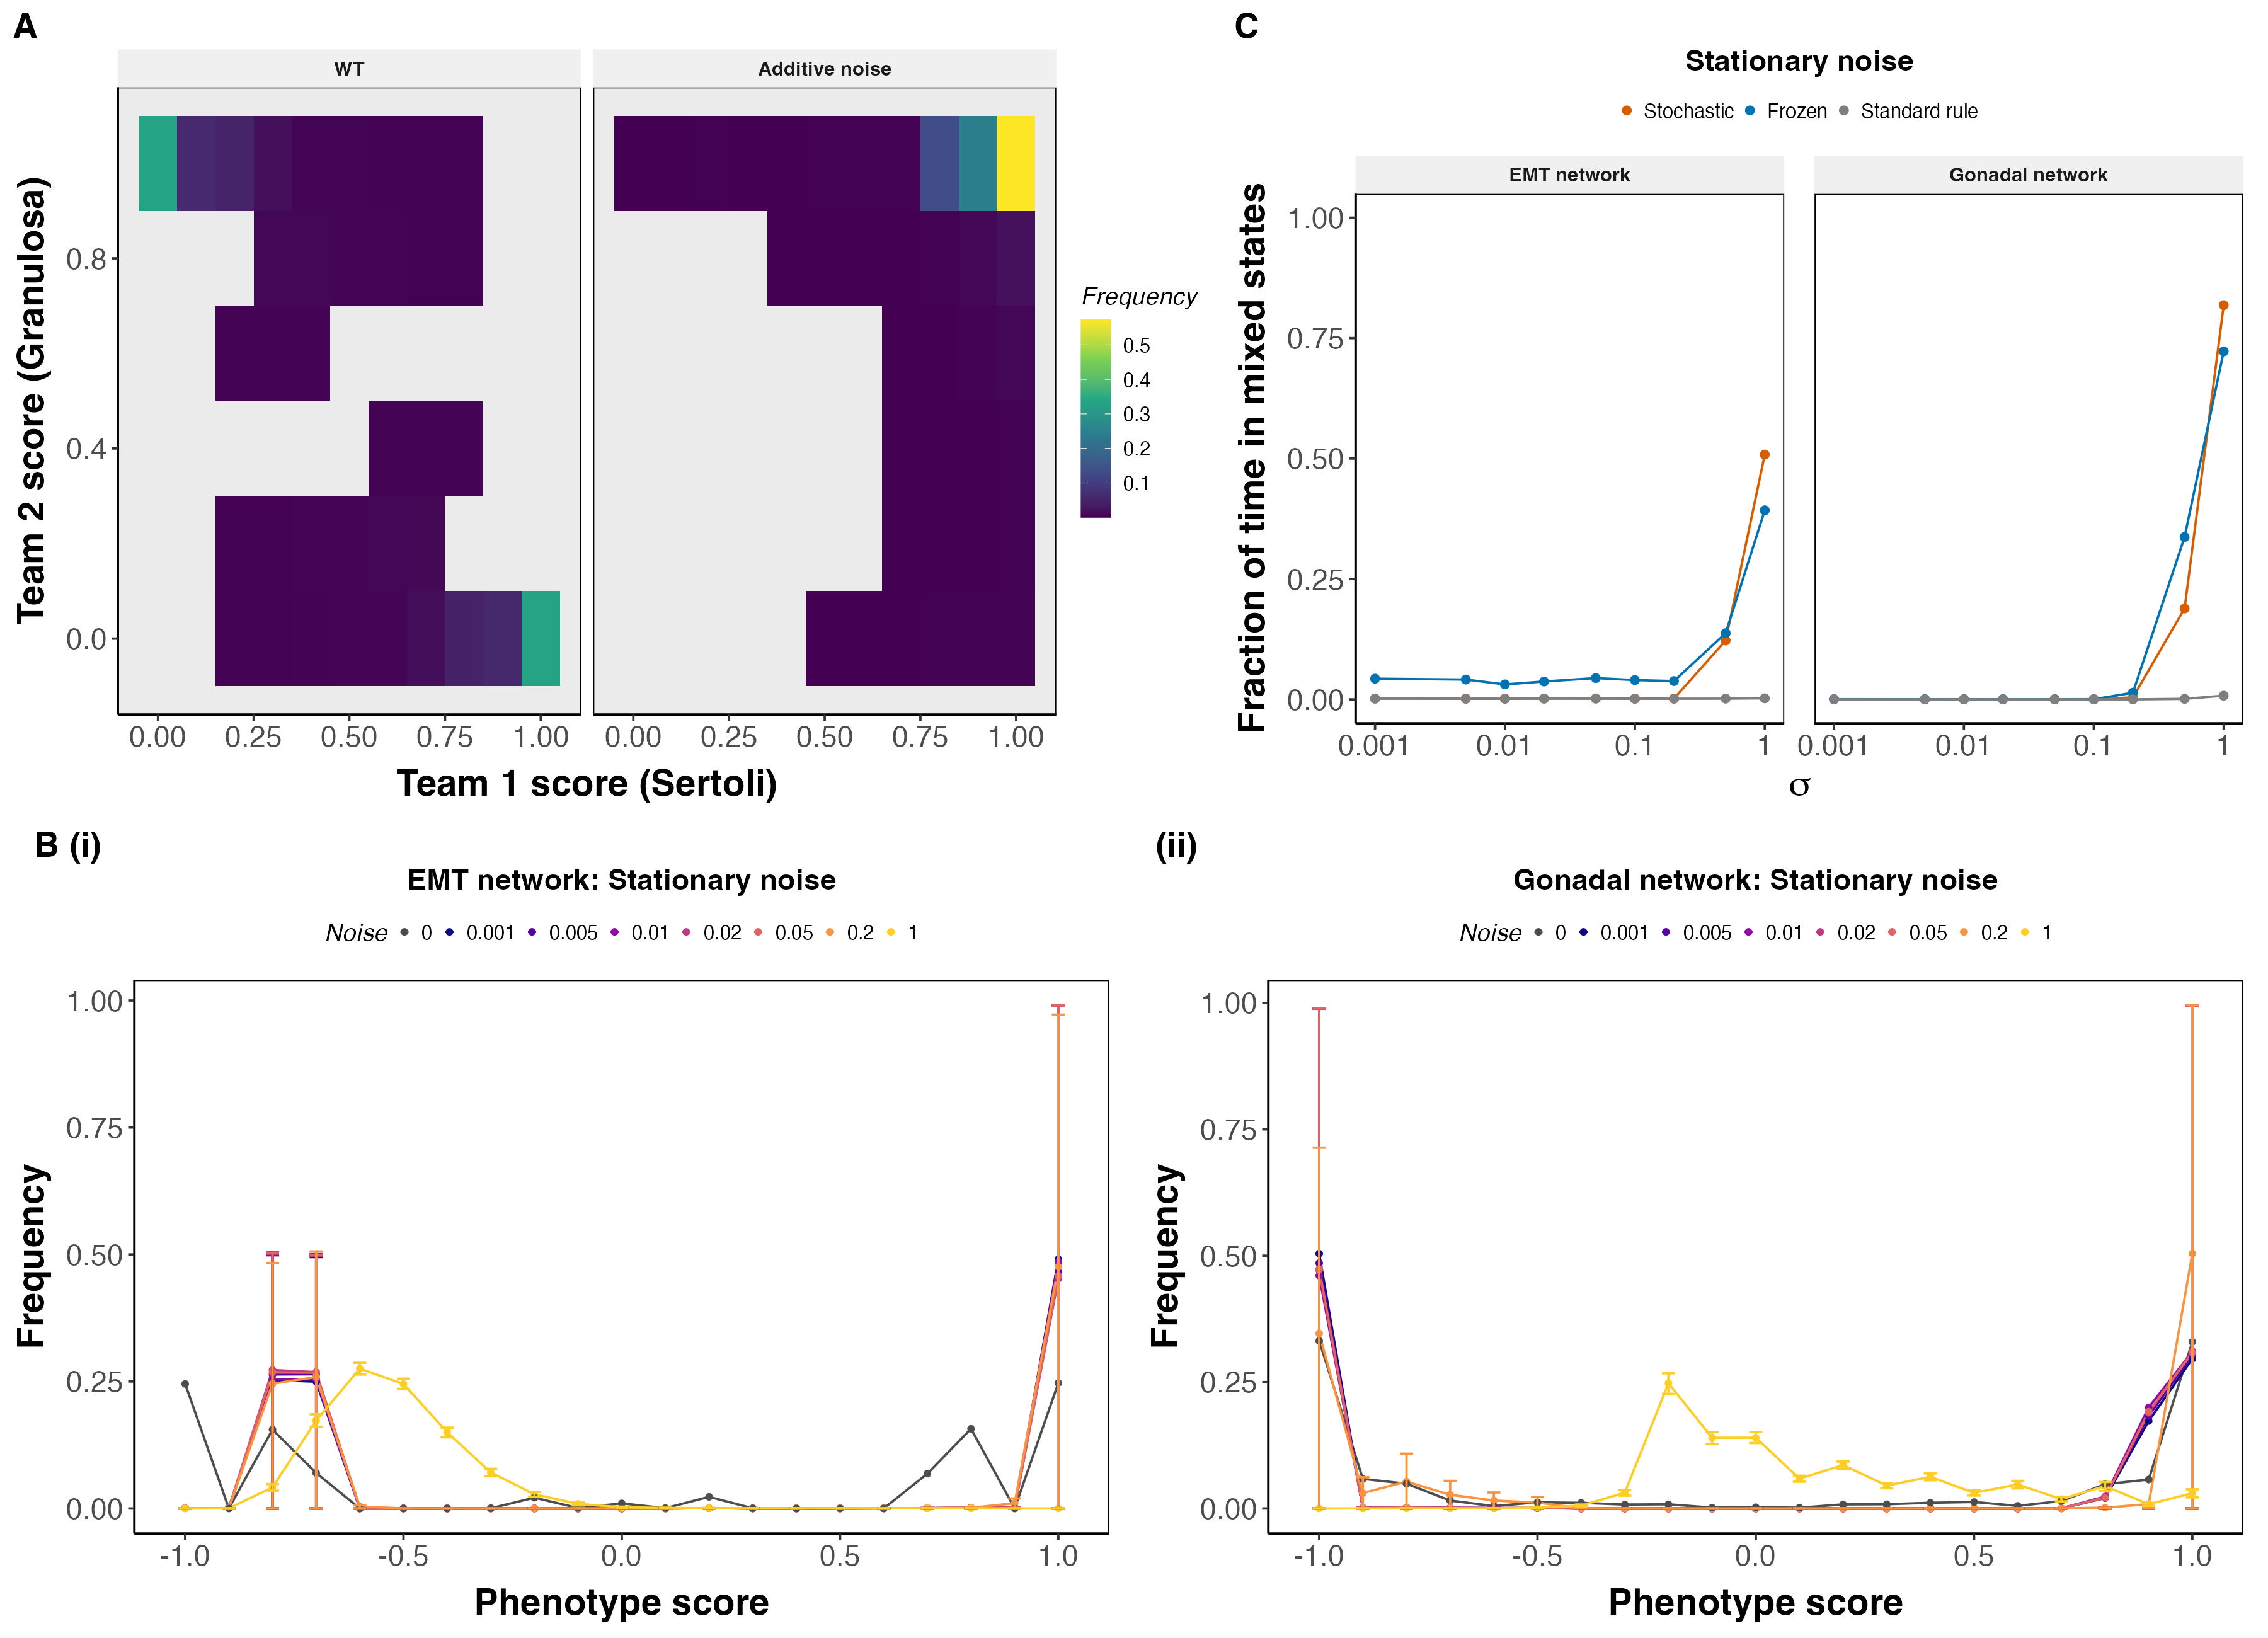
\includegraphics[width=0.8\linewidth]{Fig7S2.jpg}
    \caption{\textbf{Gonadal team-score density and stationary noise in the Boolean models.}
    A) Team-score density for the gonadal network, displayed as in Figure~\ref{fig:7}B: steady states of the
    unperturbed network (WT) and stochastic trajectories under additive noise at $\sigma = 0.05$ (ODE-equivalent
    threshold rule, Eq.~\ref{eq:boolbias}). B) Fraction of time at each phenotypic score under stationary noise,
    mean and interquartile range over 1000 trajectories, for the (i) EMT and (ii) gonadal networks, as in Figure~\ref{fig:7}C.
    C) Fraction of time in mixed states against $\sigma$ under stationary noise, for stochastic weights, frozen weights and the standard threshold rule, as in Figure~\ref{fig:7}D.}
    \label{fig:7S2}
\end{figure}

\newpage
\clearpage
\section{Supplementary Tables}

\begin{table}[!ht]
\centering
\caption{\normalsize{Threshold values used to discretize node expressions for different states in small cell-fate network motifs}}
\label{tb:Thresholds}
\begin{tabular}{|c|c|c|}
    \hline
    \textbf{Node} &  \textbf{Threshold} & \textbf{Network}\\
    \hline\hline
    A & 16.95 & Toggle Switch (TS)\\
    \hline
    B & 19.44 & Toggle Switch (TS)\\
    \hline
    A & 2.57 & Toggle Switch with Self-Activation (TSSA)\\
    \hline
    B & 2.73 & Toggle Switch with Self-Activation (TSSA)\\
    \hline
    A & 4.95 & Toggle Triad (TT)\\
    \hline
    B & 5.19 & Toggle Triad (TT)\\
    \hline
    C & 5.03 & Toggle Triad (TT)\\
    \hline
    A & 0.70 & Toggle Triad with Self-Activation (TTSA)\\
    \hline
    B & 0.72 & Toggle Triad with Self-Activation (TTSA)\\
    \hline
    C & 0.75 & Toggle Triad with Self-Activation (TTSA)\\
    \hline
    A & 1.19 & Toggle Tetrahedron (TT4)\\
    \hline
    B & 1.32 & Toggle Tetrahedron (TT4)\\
    \hline
    C & 1.30 & Toggle Tetrahedron (TT4)\\
    \hline
    D & 1.28 & Toggle Tetrahedron (TT4)\\
    \hline
    A & 0.16 & Toggle Tetrahedron with Self-Activation (TT4SA)\\
    \hline
    B & 0.16 & Toggle Tetrahedron with Self-Activation (TT4SA)\\
    \hline
    C & 0.16 & Toggle Tetrahedron with Self-Activation (TT4SA)\\
    \hline
    D & 0.17 & Toggle Tetrahedron with Self-Activation (TT4SA)\\
    \hline
    A & 3.14 & Coupled Toggle Switches (TS4)\\
    \hline
    B & 3.08 & Coupled Toggle Switches (TS4)\\
    \hline
    C & 3.10 & Coupled Toggle Switches (TS4)\\
    \hline
    D & 3.11 & Coupled Toggle Switches (TS4)\\
    \hline
\end{tabular}
\end{table}


\noindent
\refstepcounter{table}
\label{tb:Attractors}
\begin{center}
  \small{\textbf{Table~\thetable: }}Attractor frequencies across all network motifs.
  Each sub-panel lists attractors (monostable or multistable, written as
  state-tuples joined by ``\_'') and their frequencies in RACIPE.
\end{center}

\medskip

%% ── Row 1: six 2-node networks ──────────────────────────────────────────
\noindent
\begin{minipage}[t]{0.45\linewidth}
\begin{tabular}{@{}lr@{}}
\multicolumn{2}{@{}l}{\textbf{(a) Toggle Switch (TS)}}\\
\toprule
Attractor & Freq.\\
\midrule
(0,1)          & 0.3744 \\
(1,0)          & 0.3318 \\
(0,1)\_(1,0)   & 0.1858 \\
(1,1)          & 0.0573 \\
\bottomrule
\end{tabular}
\end{minipage}
\hfill
\begin{minipage}[t]{0.45\linewidth}
\begin{tabular}{@{}lr@{}}
\multicolumn{2}{@{}l}{\textbf{(b) TS Self-Activation (TSSA)}}\\
\toprule
Attractor & Freq.\\
\midrule
(0,1)\_(1,0)           & 0.4865 \\
(0,1)                  & 0.1357 \\
(1,0)                  & 0.1243 \\
(0,0)\_(0,1)\_(1,0)    & 0.0682 \\
(0,1)\_(1,0)\_(1,1)    & 0.0369 \\
(1,0)\_(1,1)           & 0.0284 \\
(0,1)\_(1,1)           & 0.0254 \\
(0,0)\_(0,1)           & 0.0187 \\
(0,0)\_(1,0)           & 0.0184 \\
\bottomrule
\end{tabular}
\end{minipage}
\medskip

%% ── Row 2: Toggle Triad and NF Self-Activation ──────────────────────────
\noindent
\begin{minipage}[t]{0.47\linewidth}
\begin{tabular}{@{}lr@{}}
\multicolumn{2}{@{}l}{\textbf{(g) Toggle Triad (TT)}}\\
\toprule
Attractor & Freq.\\
\midrule
(0,0,1)                                    & 0.1312 \\
(0,1,0)                                    & 0.1241 \\
(1,0,0)                                    & 0.1184 \\
(0,0,1)\_(0,1,0)                           & 0.0694 \\
(0,1,0)\_(1,0,0)                           & 0.0638 \\
(0,0,1)\_(1,0,0)                           & 0.0632 \\
(1,0,1)                                    & 0.0567 \\
(1,1,0)                                    & 0.0559 \\
(0,1,1)                                    & 0.0535 \\
(0,0,1)\_(0,1,0)\_(1,0,0)                 & 0.0206 \\
(0,1,0)\_(1,0,1)                           & 0.0187 \\
(1,0,0)\_(1,0,1)                           & 0.0181 \\
(0,1,0)\_(0,1,1)                           & 0.0171 \\
(1,0,0)\_(1,1,0)                           & 0.0169 \\
(0,1,1)\_(1,0,0)                           & 0.0166 \\
(0,0,1)\_(1,1,0)                           & 0.0161 \\
(0,1,0)\_(1,1,0)                           & 0.0146 \\
(0,0,1)\_(1,0,1)                           & 0.0138 \\
(0,0,1)\_(0,1,1)                           & 0.0136 \\
(0,1,1)\_(1,1,0)                           & 0.0078 \\
(1,0,1)\_(1,1,0)                           & 0.0078 \\
(0,1,1)\_(1,0,1)                           & 0.0076 \\
(1,0,1)\_(1,0,1)                           & 0.0055 \\
(1,1,0)\_(1,1,0)                           & 0.0042 \\
(0,1,0)\_(1,0,0)\_(1,0,1)                 & 0.0039 \\
(0,0,1)\_(1,0,0)\_(1,1,0)                 & 0.0037 \\
(0,1,1)\_(0,1,1)                           & 0.0034 \\
(0,0,1)\_(0,1,0)\_(1,1,0)                 & 0.0028 \\
\bottomrule
\end{tabular}
\end{minipage}
\hfill
\begin{minipage}[t]{0.45\linewidth}
\begin{tabular}{@{}lr@{}}
\multicolumn{2}{@{}l}{\textbf{(j) Coupled Toggle Switches (TS4)}}\\
\toprule
Attractor & Freq.\\
\midrule
(0,1,0,1)\_(1,0,1,0)                               & 0.5244 \\
(1,0,1,0)                                          & 0.1313 \\
(0,1,0,1)                                          & 0.1251 \\
(0,1,0,1)\_(1,0,1,1)                               & 0.0112 \\
(1,0,1,0)\_(1,1,0,1)                               & 0.0108 \\
(0,1,0,1)\_(1,1,1,0)                               & 0.0096 \\
(0,1,1,1)\_(1,0,1,0)                               & 0.0096 \\
(0,1,0,1)\_(1,0,1,0)\_(1,1,0,0)                   & 0.0093 \\
(0,0,1,1)\_(0,1,0,1)\_(1,0,1,0)                   & 0.0092 \\
(0,1,0,1)\_(1,0,0,1)\_(1,0,1,0)                   & 0.0092 \\
(0,1,0,1)\_(0,1,1,0)\_(1,0,1,0)                   & 0.0088 \\
(0,1,0,1)\_(0,1,1,1)\_(1,0,1,0)                   & 0.0079 \\
(0,1,0,1)\_(1,0,1,0)\_(1,0,1,1)                   & 0.0065 \\
(0,1,0,1)\_(1,0,1,0)\_(1,1,1,0)                   & 0.0063 \\
(0,1,0,1)\_(1,0,1,0)\_(1,1,0,1)                   & 0.0059 \\
(0,1,0,1)\_(1,0,0,0)                               & 0.0049 \\
(0,1,0,0)\_(1,0,1,0)                               & 0.0042 \\
(0,0,1,0)\_(0,1,0,1)                               & 0.0041 \\
(0,1,0,1)\_(0,1,1,0)                               & 0.0040 \\
(0,1,0,1)\_(1,0,0,1)                               & 0.0040 \\
(0,1,0,1)\_(1,1,0,0)                               & 0.0040 \\
(1,0,0,1)\_(1,0,1,0)                               & 0.0040 \\
(0,1,0,1)\_(1,0,0,0)\_(1,0,1,0)                   & 0.0038 \\
(0,0,0,1)\_(1,0,1,0)                               & 0.0037 \\
(0,1,1,0)\_(1,0,1,0)                               & 0.0037 \\
(1,0,1,0)\_(1,1,0,0)                               & 0.0037 \\
(0,0,1,1)\_(1,0,1,0)                               & 0.0036 \\
(0,1,0,1)\_(0,1,0,1)\_(1,0,1,0)                   & 0.0035 \\
(0,0,1,1)\_(0,1,0,1)                               & 0.0034 \\
(0,0,0,1)\_(0,1,0,1)\_(1,0,1,0)                   & 0.0033 \\
(0,1,0,0)\_(0,1,0,1)\_(1,0,1,0)                   & 0.0032 \\
(1,0,1,0)\_(1,1,1,0)                               & 0.0032 \\
\bottomrule
\end{tabular}
\end{minipage}



\bigskip

%% ── Row 4: TTSA across three columns ─────────────────────────────────────
\noindent
\begin{minipage}[t]{\linewidth}
\begin{tabular}{@{}lr@{}}
\multicolumn{2}{@{}l}{\textbf{(i) Toggle Triad SA (TTSA) — cont'd across columns}}\\
\toprule
Attractor & Freq.\\
\midrule
(0,0,1)\_(0,1,0)\_(1,0,0)                         & 0.1449 \\
(0,0,1)\_(0,1,0)                                   & 0.0459 \\
(0,0,1)\_(1,0,0)                                   & 0.0444 \\
(0,1,0)\_(1,0,0)                                   & 0.0444 \\
(1,0,0)                                            & 0.0362 \\
(0,0,1)                                            & 0.0359 \\
(0,1,0)                                            & 0.0330 \\
(0,0,1)\_(0,1,0)\_(1,0,0)\_(1,0,1)                & 0.0228 \\
(1,0,0)\_(1,0,1)                                   & 0.0227 \\
(0,0,1)\_(0,1,0)\_(0,1,1)\_(1,0,0)                & 0.0220 \\
(0,0,1)\_(0,1,1)                                   & 0.0215 \\
(0,1,0)\_(0,1,1)                                   & 0.0213 \\
(0,1,0)\_(1,1,0)                                   & 0.0203 \\
(0,0,1)\_(0,1,0)\_(1,0,0)\_(1,1,0)                & 0.0201 \\
(0,0,1)\_(1,0,1)                                   & 0.0198 \\
(1,0,0)\_(1,1,0)                                   & 0.0195 \\
(0,1,1)                                            & 0.0188 \\
(1,0,1)                                            & 0.0183 \\
(0,0,1)\_(0,1,0)\_(0,1,1)                         & 0.0166 \\
(1,1,0)                                            & 0.0161 \\
(0,0,1)\_(1,0,0)\_(1,0,1)                         & 0.0140 \\
(0,1,0)\_(1,0,0)\_(1,1,0)                         & 0.0138 \\
(1,0,0)\_(1,0,1)\_(1,1,0)                         & 0.0135 \\
(0,1,0)\_(0,1,1)\_(1,1,0)                         & 0.0132 \\
(0,0,1)\_(0,1,1)\_(1,0,1)                         & 0.0117 \\
(1,0,1)\_(1,1,0)                                   & 0.0116 \\
(0,0,1)\_(0,1,0)\_(1,0,1)                         & 0.0111 \\
(0,0,1)\_(0,1,1)\_(1,0,0)                         & 0.0110 \\
(0,1,1)\_(1,1,0)                                   & 0.0102 \\
(0,0,1)\_(0,1,0)\_(1,1,0)                         & 0.0101 \\
(0,1,1)\_(1,0,1)                                   & 0.0100 \\
(0,1,0)\_(0,1,1)\_(1,0,0)                         & 0.0098 \\
(0,1,0)\_(1,0,0)\_(1,0,1)                         & 0.0097 \\
(0,0,1)\_(1,0,0)\_(1,1,0)                         & 0.0096 \\
\bottomrule
\end{tabular}
\end{minipage}
\hfill
\begin{minipage}[t]{\linewidth}
\begin{tabular}{@{}lr@{}}
\toprule
Attractor & Freq.\\
\midrule
(0,0,1)\_(0,1,0)\_(0,1,1)\_(1,0,0)\_(1,0,1)      & 0.0073 \\
(0,1,1)\_(1,0,0)                                   & 0.0071 \\
(0,0,1)\_(0,1,0)\_(1,0,0)\_(1,0,1)\_(1,1,0)      & 0.0070 \\
(0,0,1)\_(0,1,0)\_(0,1,1)\_(1,0,0)\_(1,1,0)      & 0.0064 \\
(0,0,1)\_(1,1,0)                                   & 0.0062 \\
(0,1,1)\_(1,0,1)\_(1,1,0)                         & 0.0057 \\
(0,1,0)\_(1,0,1)                                   & 0.0055 \\
(0,0,1)\_(0,1,1)\_(1,1,0)                         & 0.0045 \\
(0,1,1)\_(1,0,0)\_(1,0,1)                         & 0.0044 \\
(0,0,1)\_(0,1,1)\_(1,0,0)\_(1,1,0)                & 0.0043 \\
(0,0,1)\_(1,0,1)\_(1,1,0)                         & 0.0043 \\
(0,1,0)\_(0,1,1)\_(1,0,0)\_(1,0,1)                & 0.0043 \\
(0,0,1)\_(0,1,0)\_(0,1,1)\_(1,0,1)                & 0.0041 \\
(0,0,1)\_(0,1,1)\_(1,0,0)\_(1,0,1)                & 0.0040 \\
(0,0,1)\_(0,1,0)\_(1,0,1)\_(1,1,0)                & 0.0035 \\
(0,1,0)\_(1,0,0)\_(1,0,1)\_(1,1,0)                & 0.0032 \\
(0,1,0)\_(1,0,1)\_(1,1,0)                         & 0.0031 \\
(0,0,1)\_(0,1,0)\_(0,1,1)\_(1,0,0)\_(1,0,1)\_(1,1,0) & 0.0030 \\
(0,1,0)\_(0,1,1)\_(1,0,1)                         & 0.0030 \\
(0,1,1)\_(1,0,0)\_(1,1,0)                         & 0.0030 \\
(0,0,1)\_(0,1,1)\_(1,0,1)\_(1,1,0)                & 0.0029 \\
(0,0,1)\_(1,0,0)\_(1,0,1)\_(1,1,0)                & 0.0029 \\
(0,1,0)\_(0,1,1)\_(1,0,1)\_(1,1,0)                & 0.0028 \\
(0,0,1)\_(0,1,0)\_(0,1,1)\_(1,1,0)                & 0.0027 \\
(0,1,0)\_(0,1,1)\_(1,0,0)\_(1,1,0)                & 0.0026 \\
(0,1,1)\_(1,0,0)\_(1,0,1)\_(1,1,0)                & 0.0026 \\
(1,1,0)\_(1,1,0)                                   & 0.0021 \\
(1,0,1)\_(1,1,1)                                   & 0.0018 \\
(0,1,0)\_(0,1,1)\_(0,1,1)                         & 0.0017 \\
(0,1,0)\_(0,1,1)\_(1,0,0)\_(1,0,1)\_(1,1,0)      & 0.0017 \\
(0,1,1)\_(0,1,1)                                   & 0.0016 \\
(1,0,1)\_(1,0,1)                                   & 0.0015 \\
(0,0,1)\_(1,0,1)\_(1,0,1)                         & 0.0014 \\
(0,1,1)\_(1,1,1)                                   & 0.0013 \\
\bottomrule
\end{tabular}
\end{minipage}
\hfill
\begin{minipage}[t]{0.45\linewidth}
\begin{tabular}{@{}lr@{}}
\toprule
Attractor & Freq.\\
\midrule
(1,0,0)\_(1,0,1)\_(1,0,1)                         & 0.0013 \\
(0,0,1)\_(0,1,1)\_(0,1,1)                         & 0.0012 \\
(0,0,1)\_(0,1,1)\_(1,0,0)\_(1,0,1)\_(1,1,0)      & 0.0012 \\
(0,1,0)\_(0,1,1)\_(1,1,0)\_(1,1,0)                & 0.0012 \\
(0,1,0)\_(1,1,0)\_(1,1,0)                         & 0.0012 \\
(0,0,1)\_(0,1,0)\_(0,1,0)\_(1,0,0)                & 0.0011 \\
(0,0,1)\_(0,1,0)\_(1,0,0)\_(1,0,0)                & 0.0011 \\
(0,0,1)\_(0,1,0)\_(1,1,0)\_(1,1,0)                & 0.0011 \\
(1,0,0)\_(1,1,0)\_(1,1,0)                         & 0.0011 \\
(1,1,0)\_(1,1,1)                                   & 0.0011 \\
(0,0,0)\_(0,0,1)\_(0,1,0)\_(1,0,0)                & 0.0010 \\
(0,1,1)\_(0,1,1)\_(1,0,1)                         & 0.0010 \\
(0,1,1)\_(0,1,1)\_(1,1,0)                         & 0.0010 \\
(0,1,1)\_(1,0,1)\_(1,1,1)                         & 0.0010 \\
(1,0,0)\_(1,0,1)\_(1,1,0)\_(1,1,1)                & 0.0010 \\
(1,0,1)\_(1,1,0)\_(1,1,0)                         & 0.0010 \\
(0,0,1)\_(0,0,1)                                   & 0.0009 \\
(0,0,1)\_(0,1,0)\_(1,0,1)\_(1,0,1)                & 0.0009 \\
(0,1,1)\_(0,1,1)\_(1,0,0)                         & 0.0009 \\
(0,1,1)\_(1,1,0)\_(1,1,1)                         & 0.0009 \\
(1,0,1)\_(1,0,1)\_(1,1,0)                         & 0.0009 \\
\bottomrule
\end{tabular}
\end{minipage}
% \begin{figure*} 
% \setlength{\tabcolsep}{2pt}
% \resizebox{1.05\textwidth}{!}{
%     \begin{tabular}{c}
%         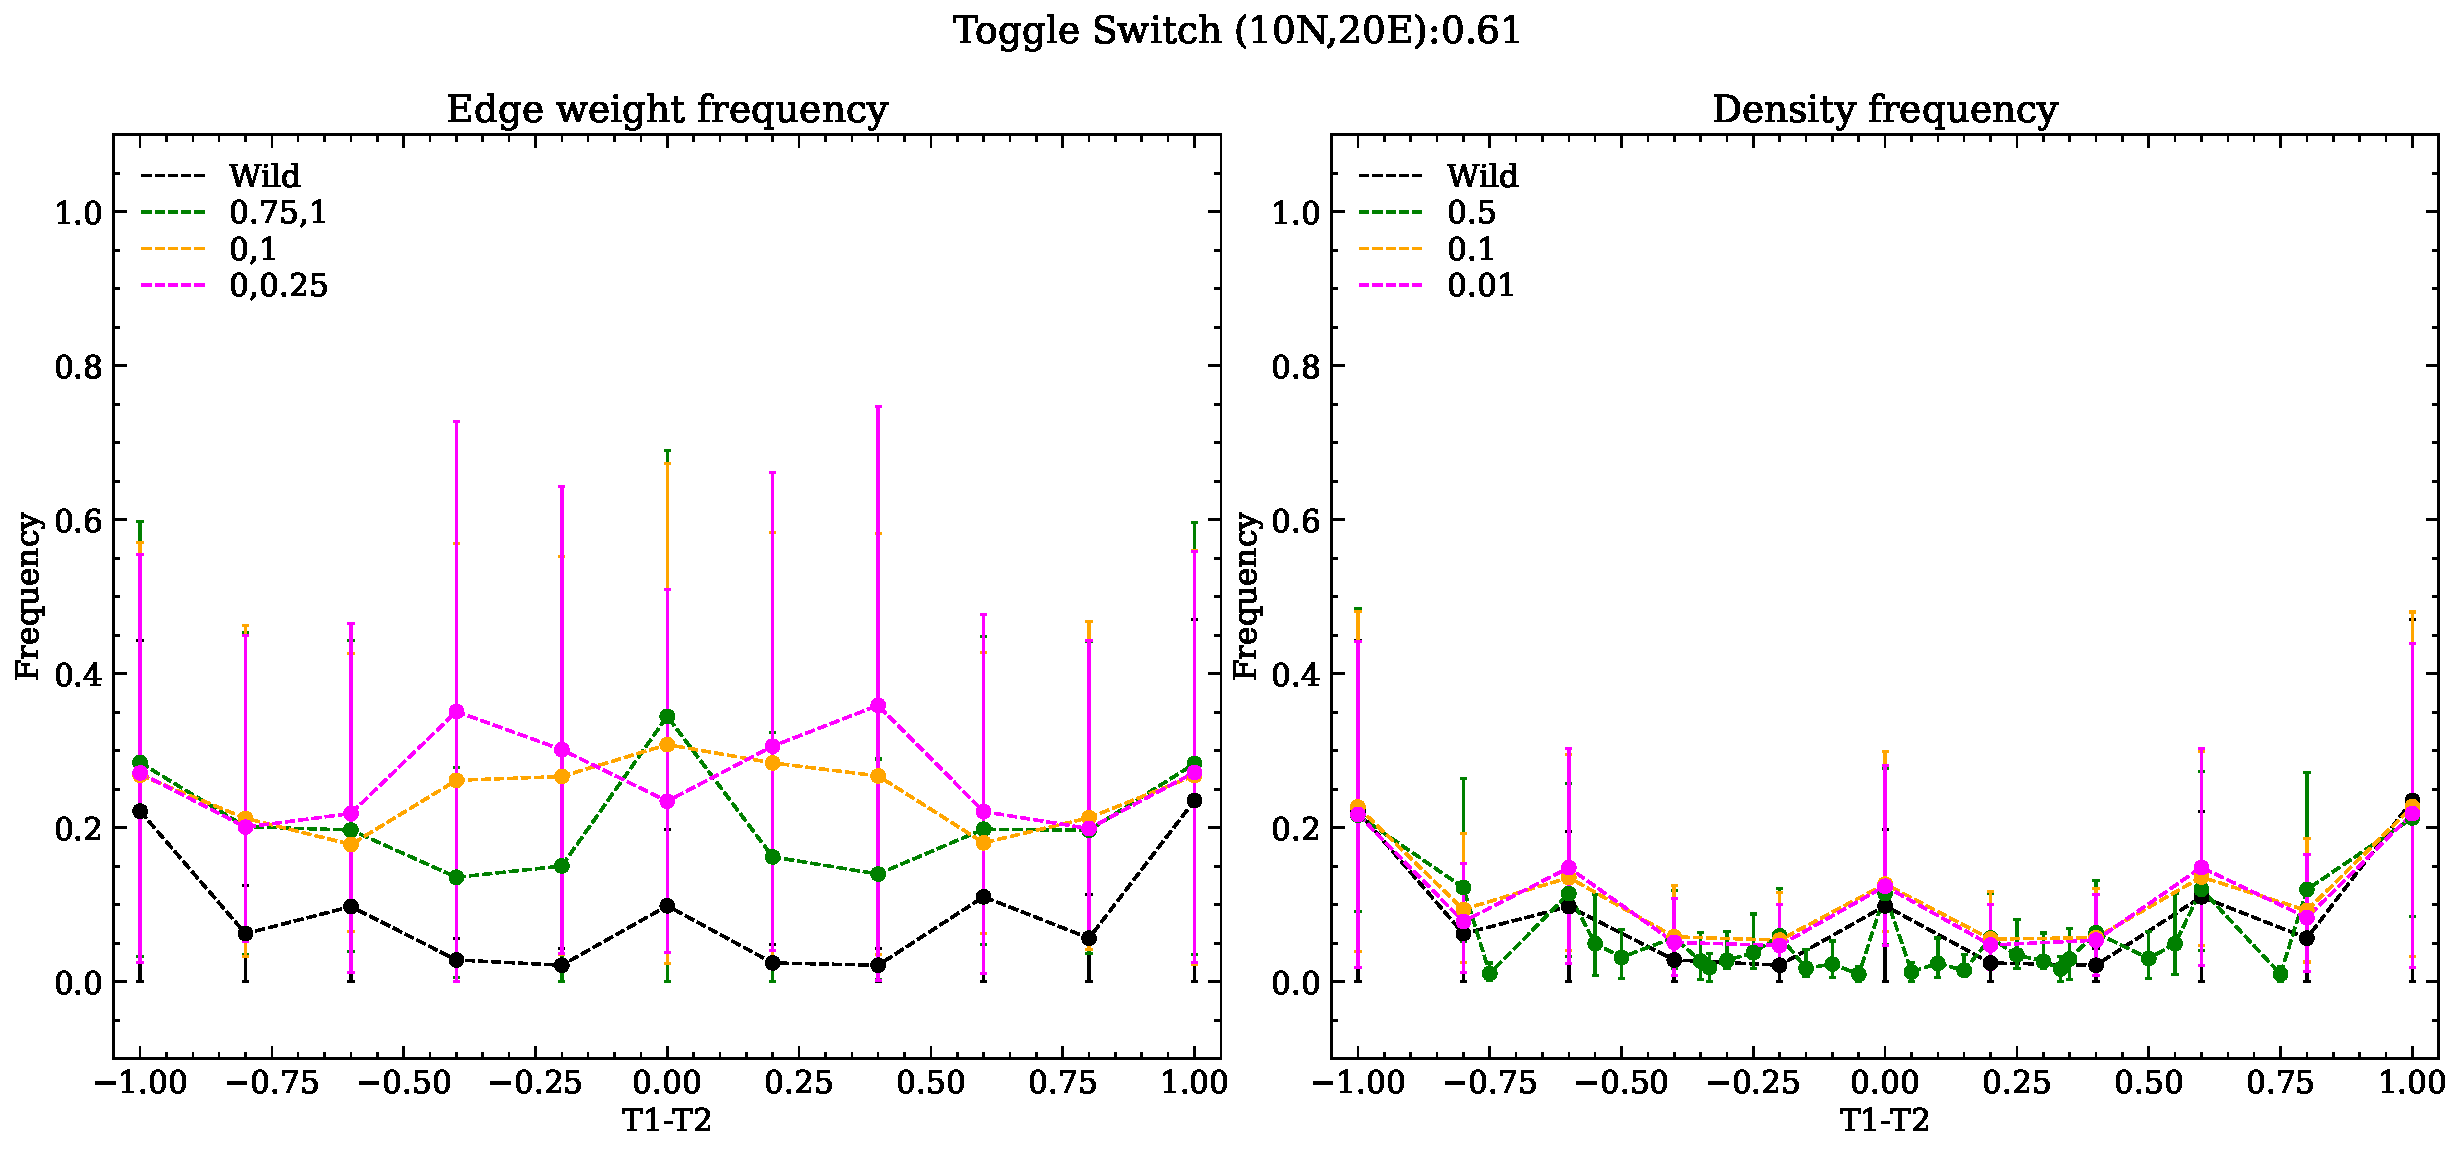
\includegraphics[height=0.3\textwidth,keepaspectratio]{Abhay_Lakshmi_old/Results/fig_1/fig1_ToggleSwitch_0.8.pdf} 
%         \\[2pt]
        
%         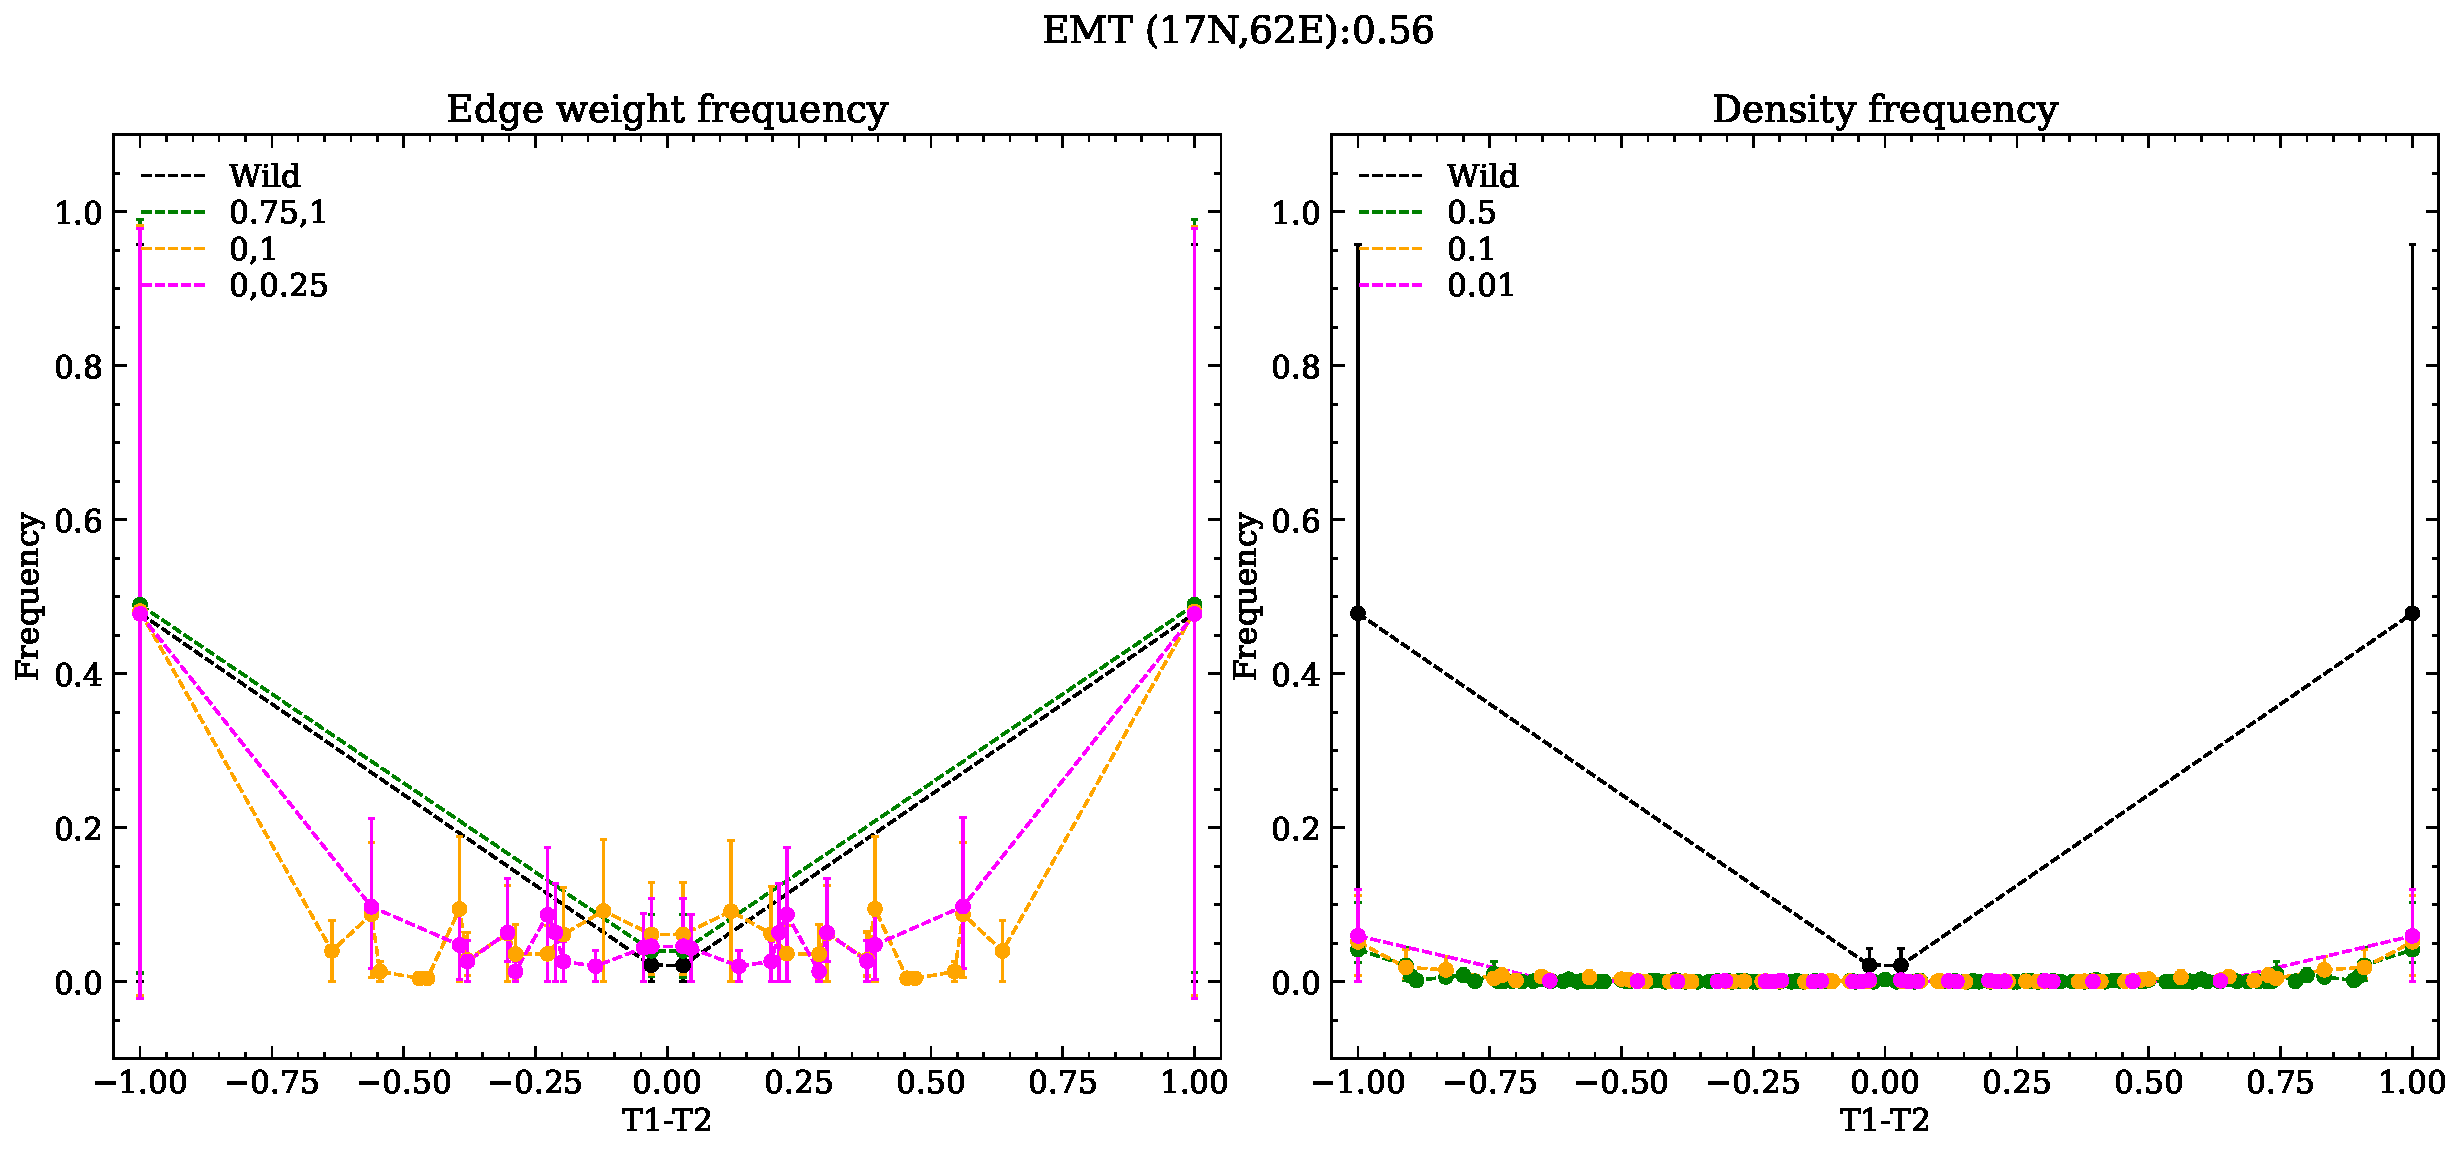
\includegraphics[height=0.3\textwidth]{Abhay_Lakshmi_old/Results/fig_1/fig1_EMT_RACIPE.pdf}\\
%     \end{tabular} 
% }
% \caption{
% \textbf{Steady-state frequencies of perturbed networks}: Steady-states are represented in terms of the difference in team expressions ($\mathrm{T1-T2}$) (x-axis);  The frequencies are for three levels of static perturbations (legend) to edge-weights (left) and density (right); The average frequencies (dots) and, the $25$-th (lower error bar) and the $75$-th (upper error bar) percentiles are displayed; The data in black belongs to the steady-state frequencies of the corresponding wild-type (unperturbed network); The top and bottom panels are of an artificial and a biological network, respectively; The titles in the panels display the network, the number of nodes and edges in the format ($x$N,$y$E) respectively, along with corresponding wild-type team strength (see Eq.~\ref{eq:ts_def}).
% Generally, static perturbations negatively affect the dominant states of a network.
% }
% \label{fig:S1}
% \end{figure*} 

% \begin{figure*}
% \setlength{\tabcolsep}{2pt}
% \resizebox{1.05\textwidth}{!}{
% \begin{tabular}{c c c c}

% \textbf{(a)} &
% {\hspace{-0.05cm}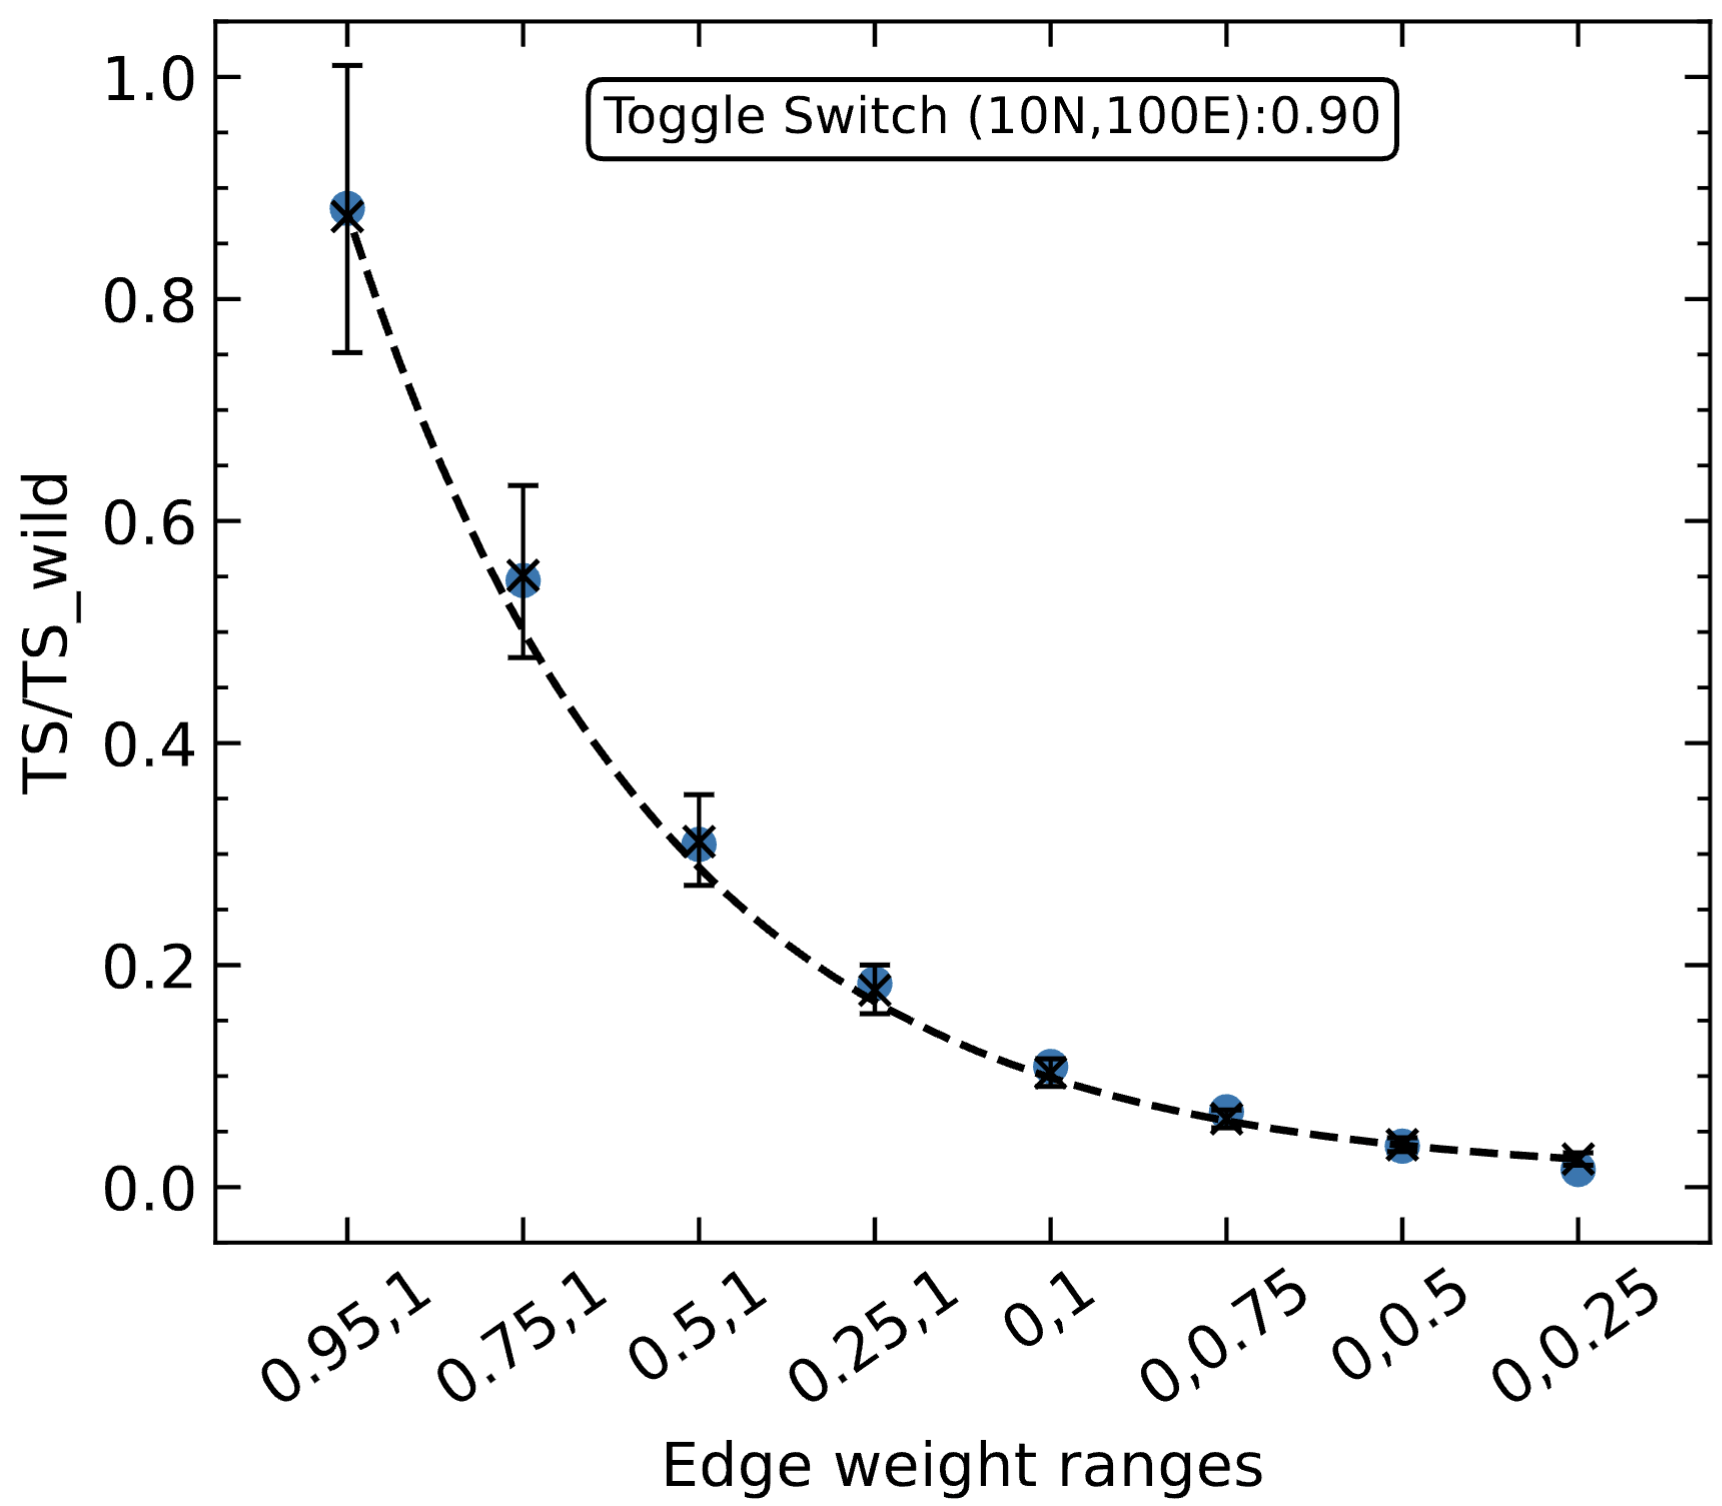
\includegraphics[width=2.83in,height=0.4\textwidth]{Abhay_Lakshmi_old/Results/ts_ew_ts.png}} &
% 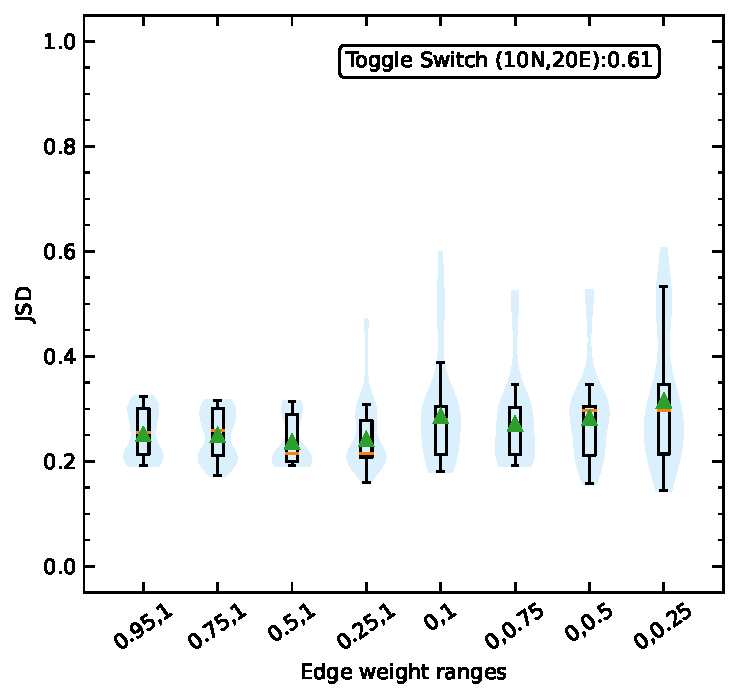
\includegraphics[width=2.85in,height=0.4\textwidth]{Abhay_Lakshmi_old/Results/JSD_compiled.pdf} &
% \textbf{(b)} \\[2pt]

% {\raisebox{0.8cm}{\hspace{-0.15cm}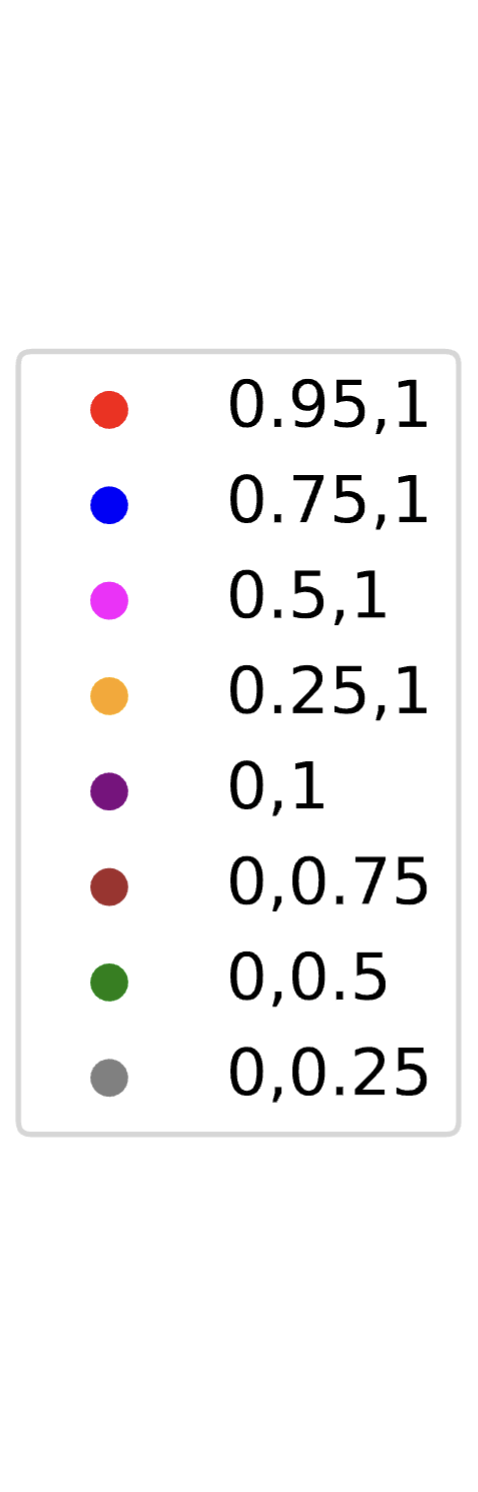
\includegraphics[height=0.3\textwidth,keepaspectratio]{Abhay_Lakshmi_old/Results/jsd_ts_net_ts.png}}} &
% {\hspace{-0.15cm}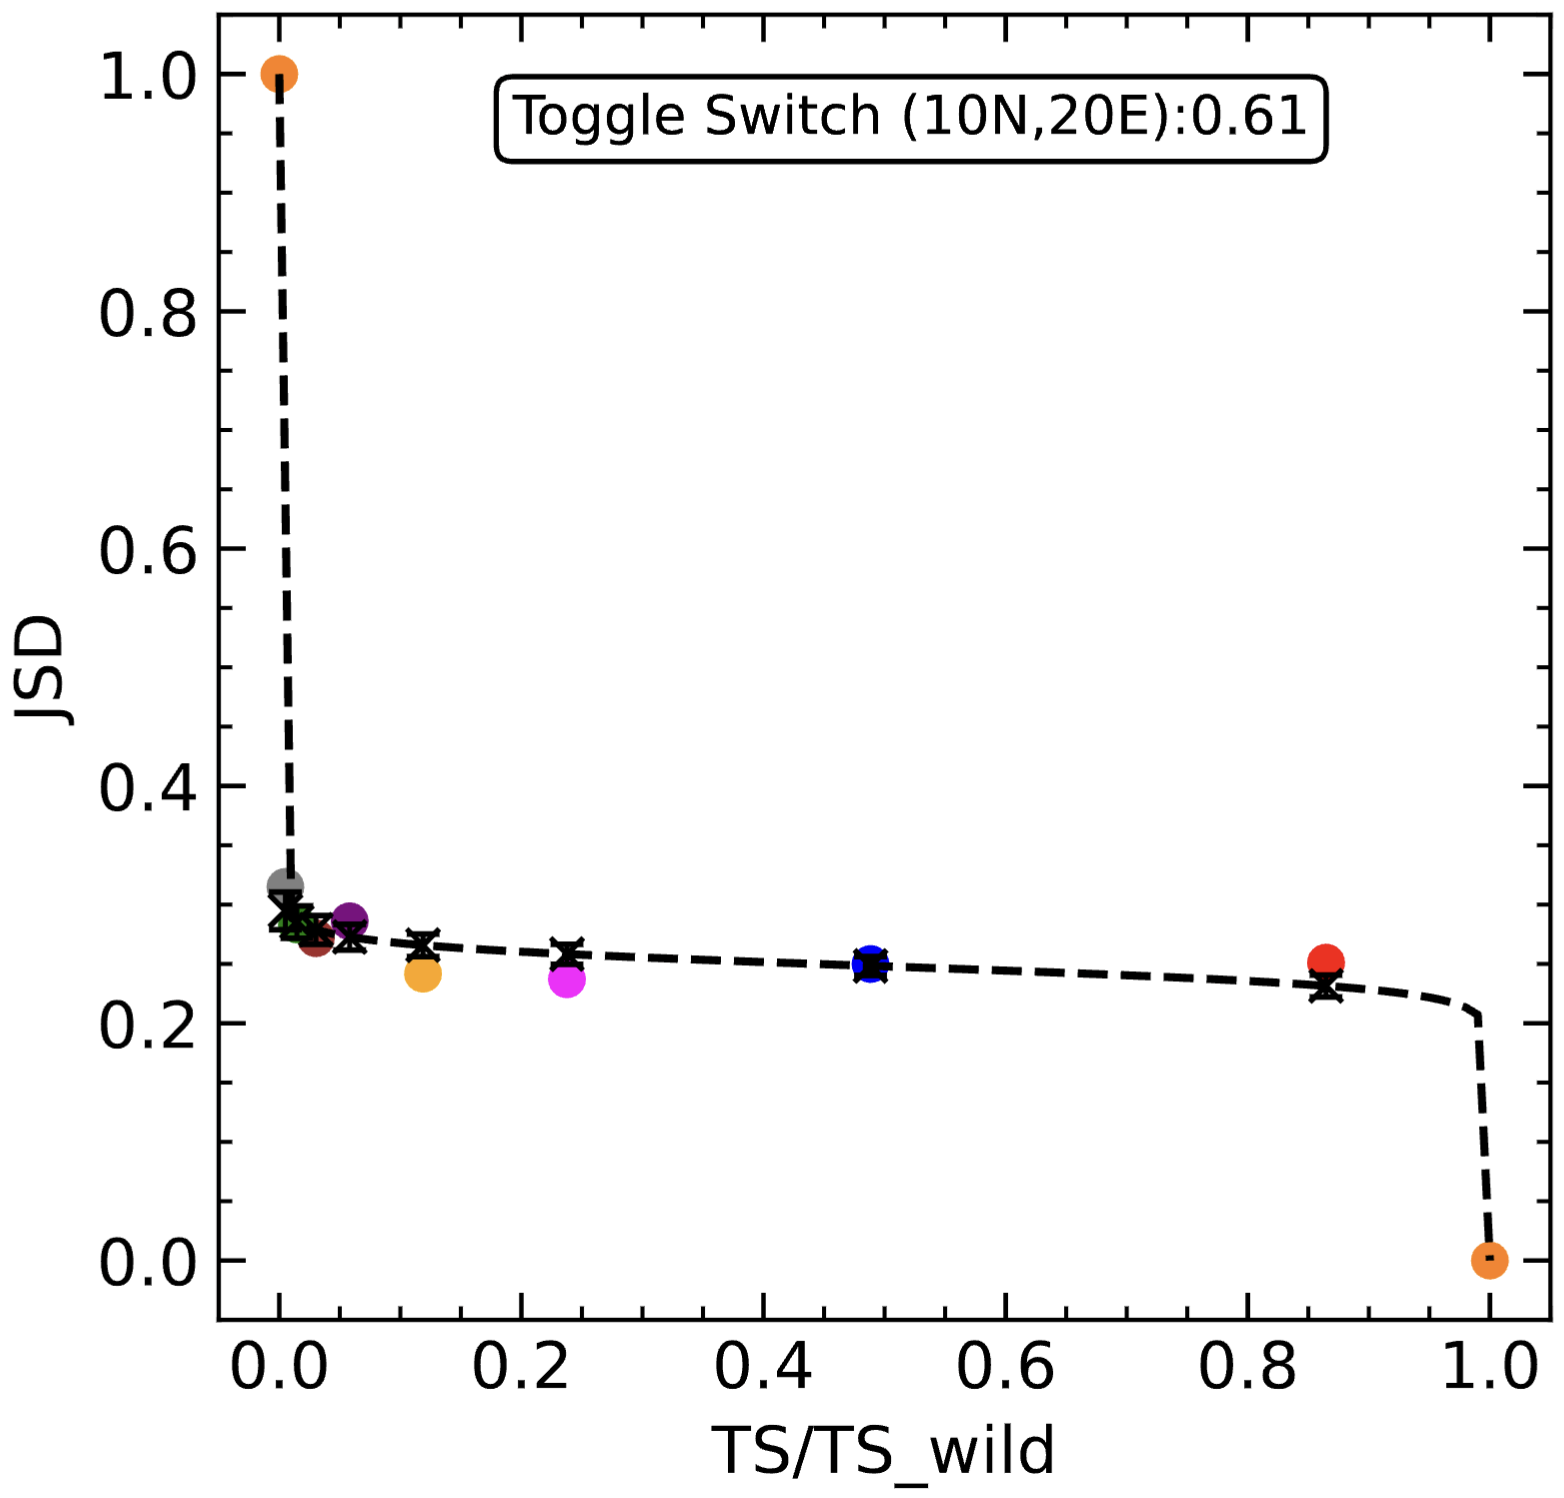
\includegraphics[width=2.9in,height=0.4\textwidth]{Abhay_Lakshmi_old/Results/jsd_ts_net_ts_fig.png}} &
% 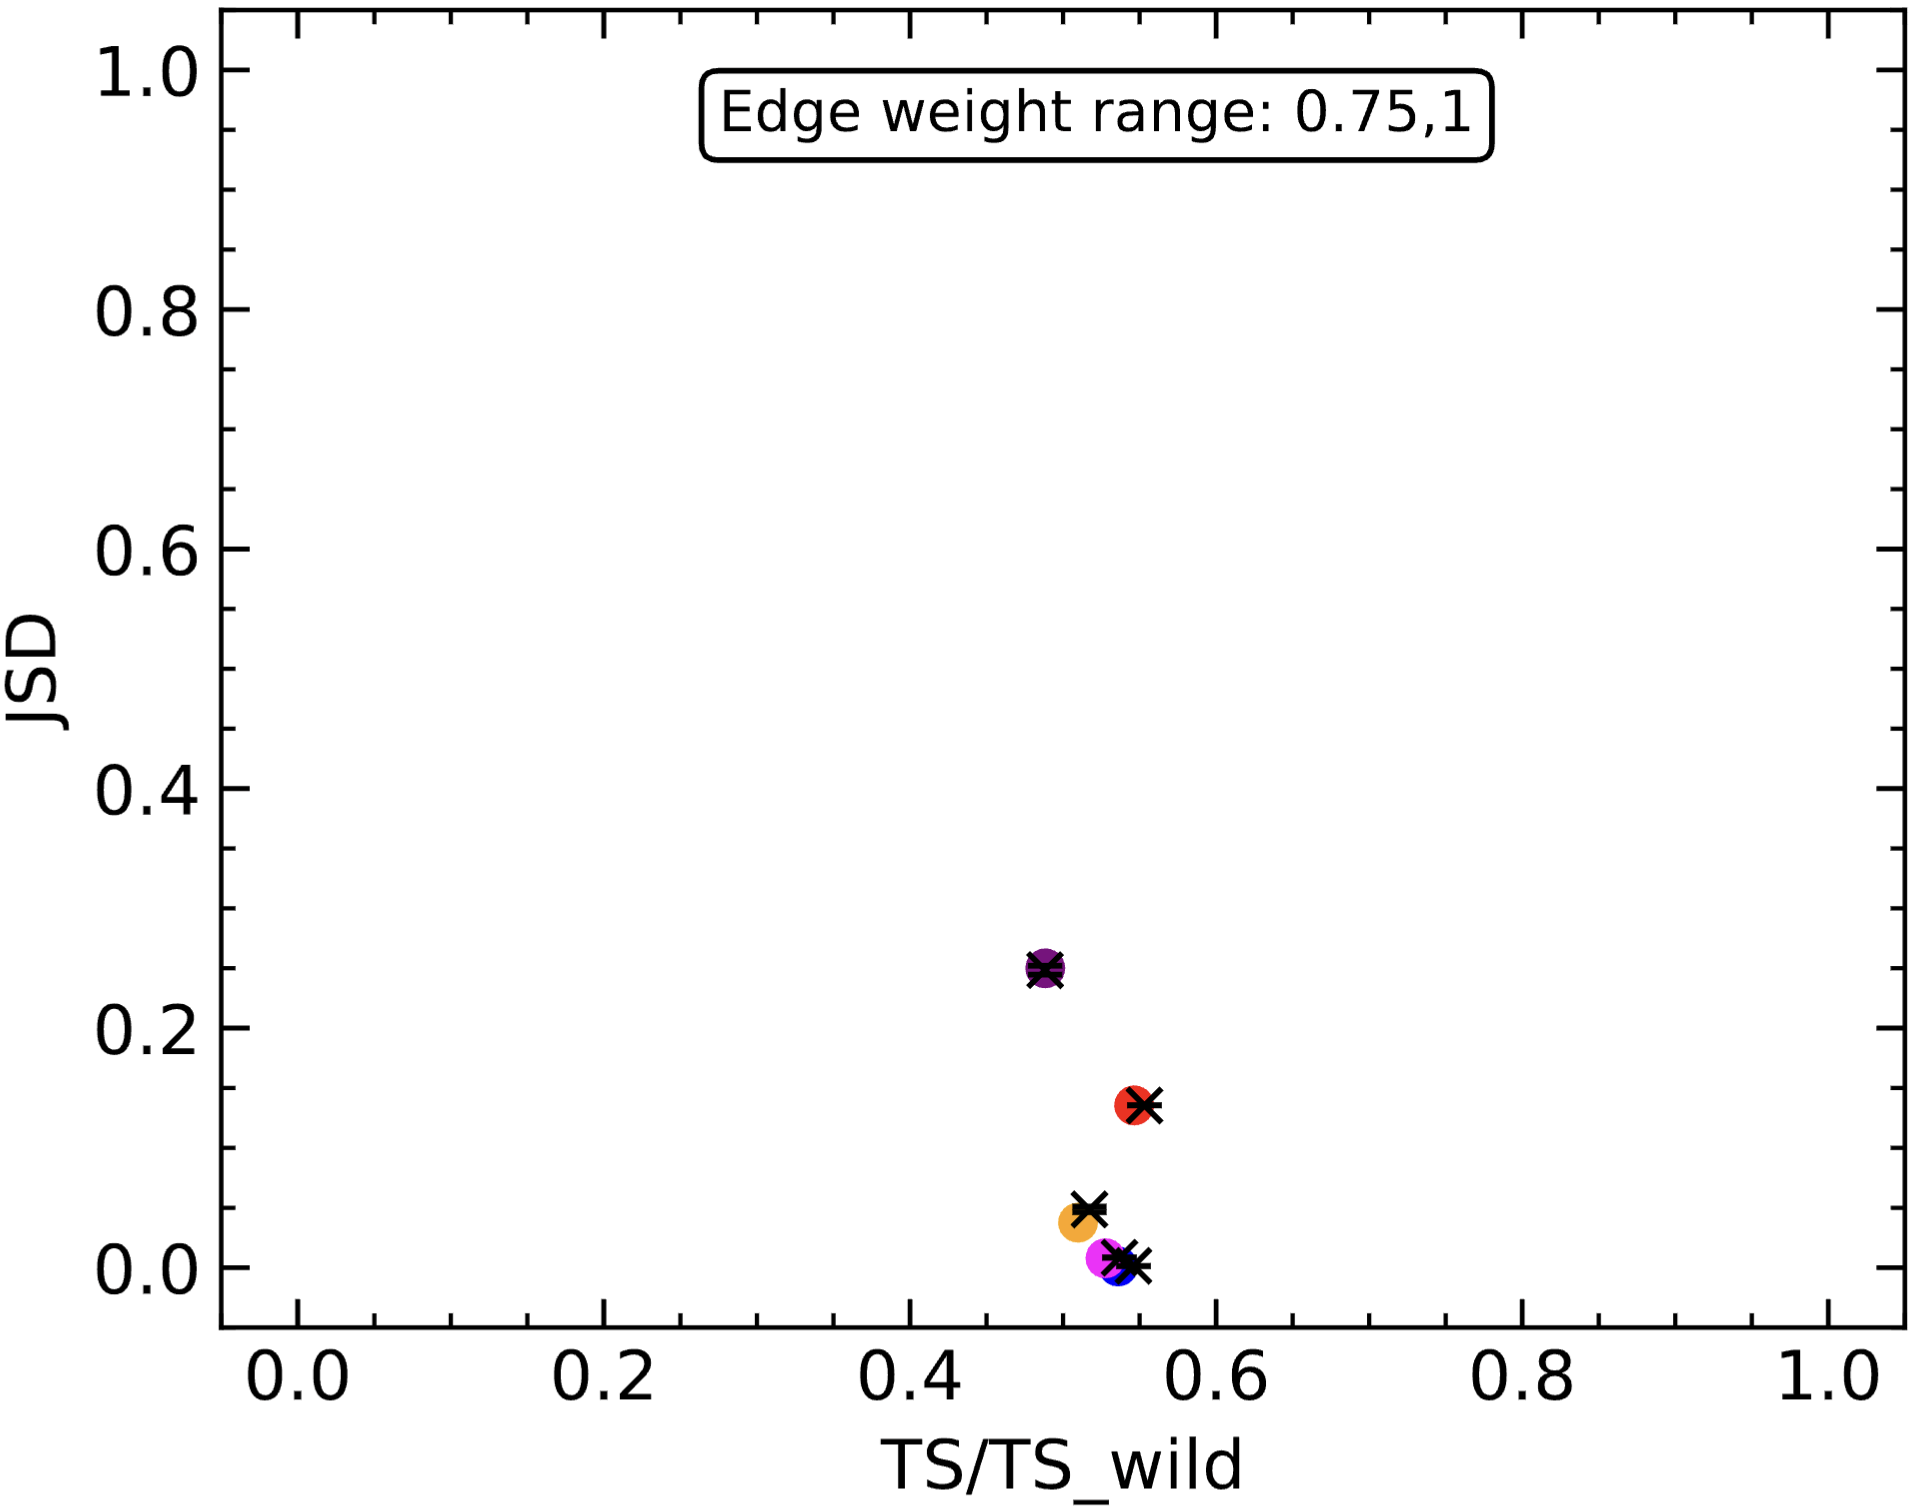
\includegraphics[height=0.4\textwidth]{Abhay_Lakshmi_old/Results/jsd_ts_ew_ts_fig.png} &
% {\raisebox{0.8cm}{\hspace{-0.15cm}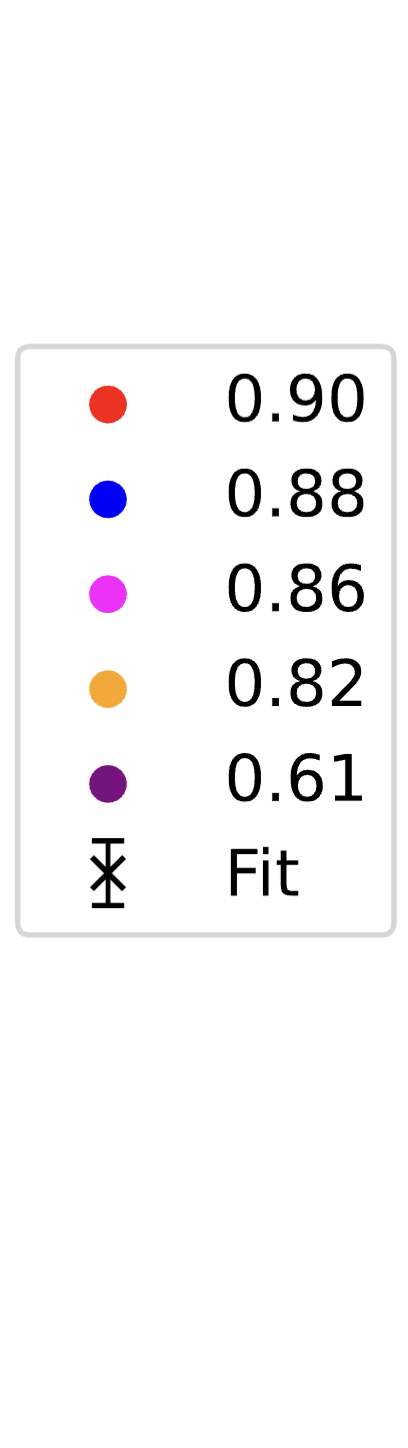
\includegraphics[height=0.3\textwidth]{Abhay_Lakshmi_old/Results/jsd_ts_ew_ts.png}}} \\[1.8pt]

% {\raisebox{0.8cm}{\hspace{-0.15cm}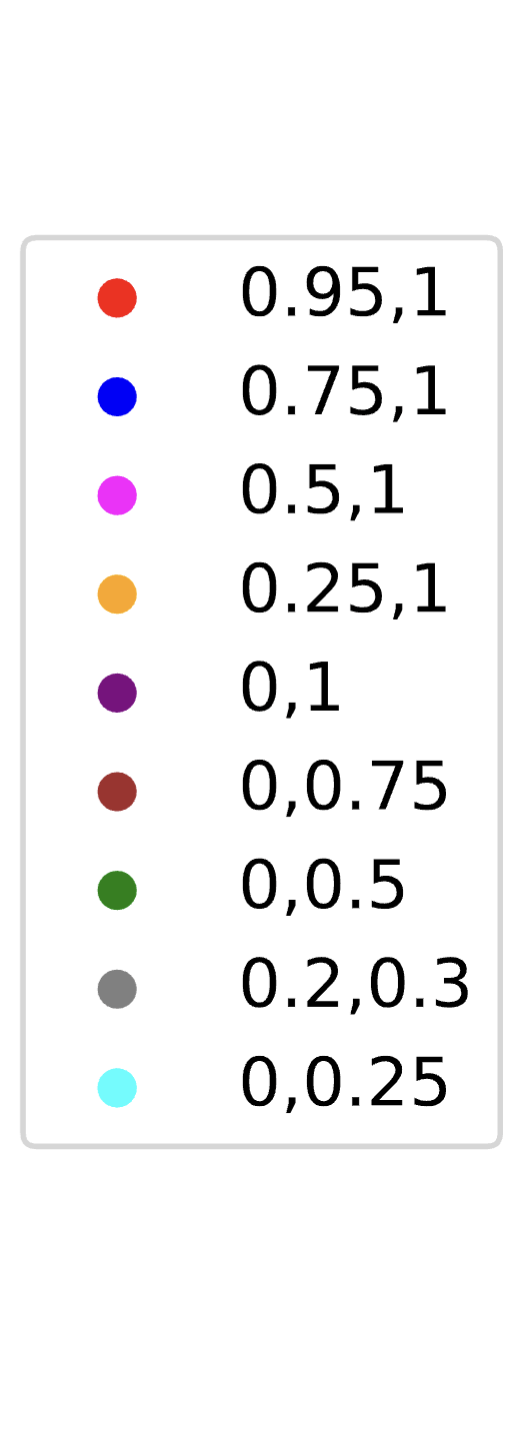
\includegraphics[height=0.3\textwidth,keepaspectratio]{Abhay_Lakshmi_old/Results/jsd_ts_net_bio.png}}} &
% {\hspace{-0.05cm}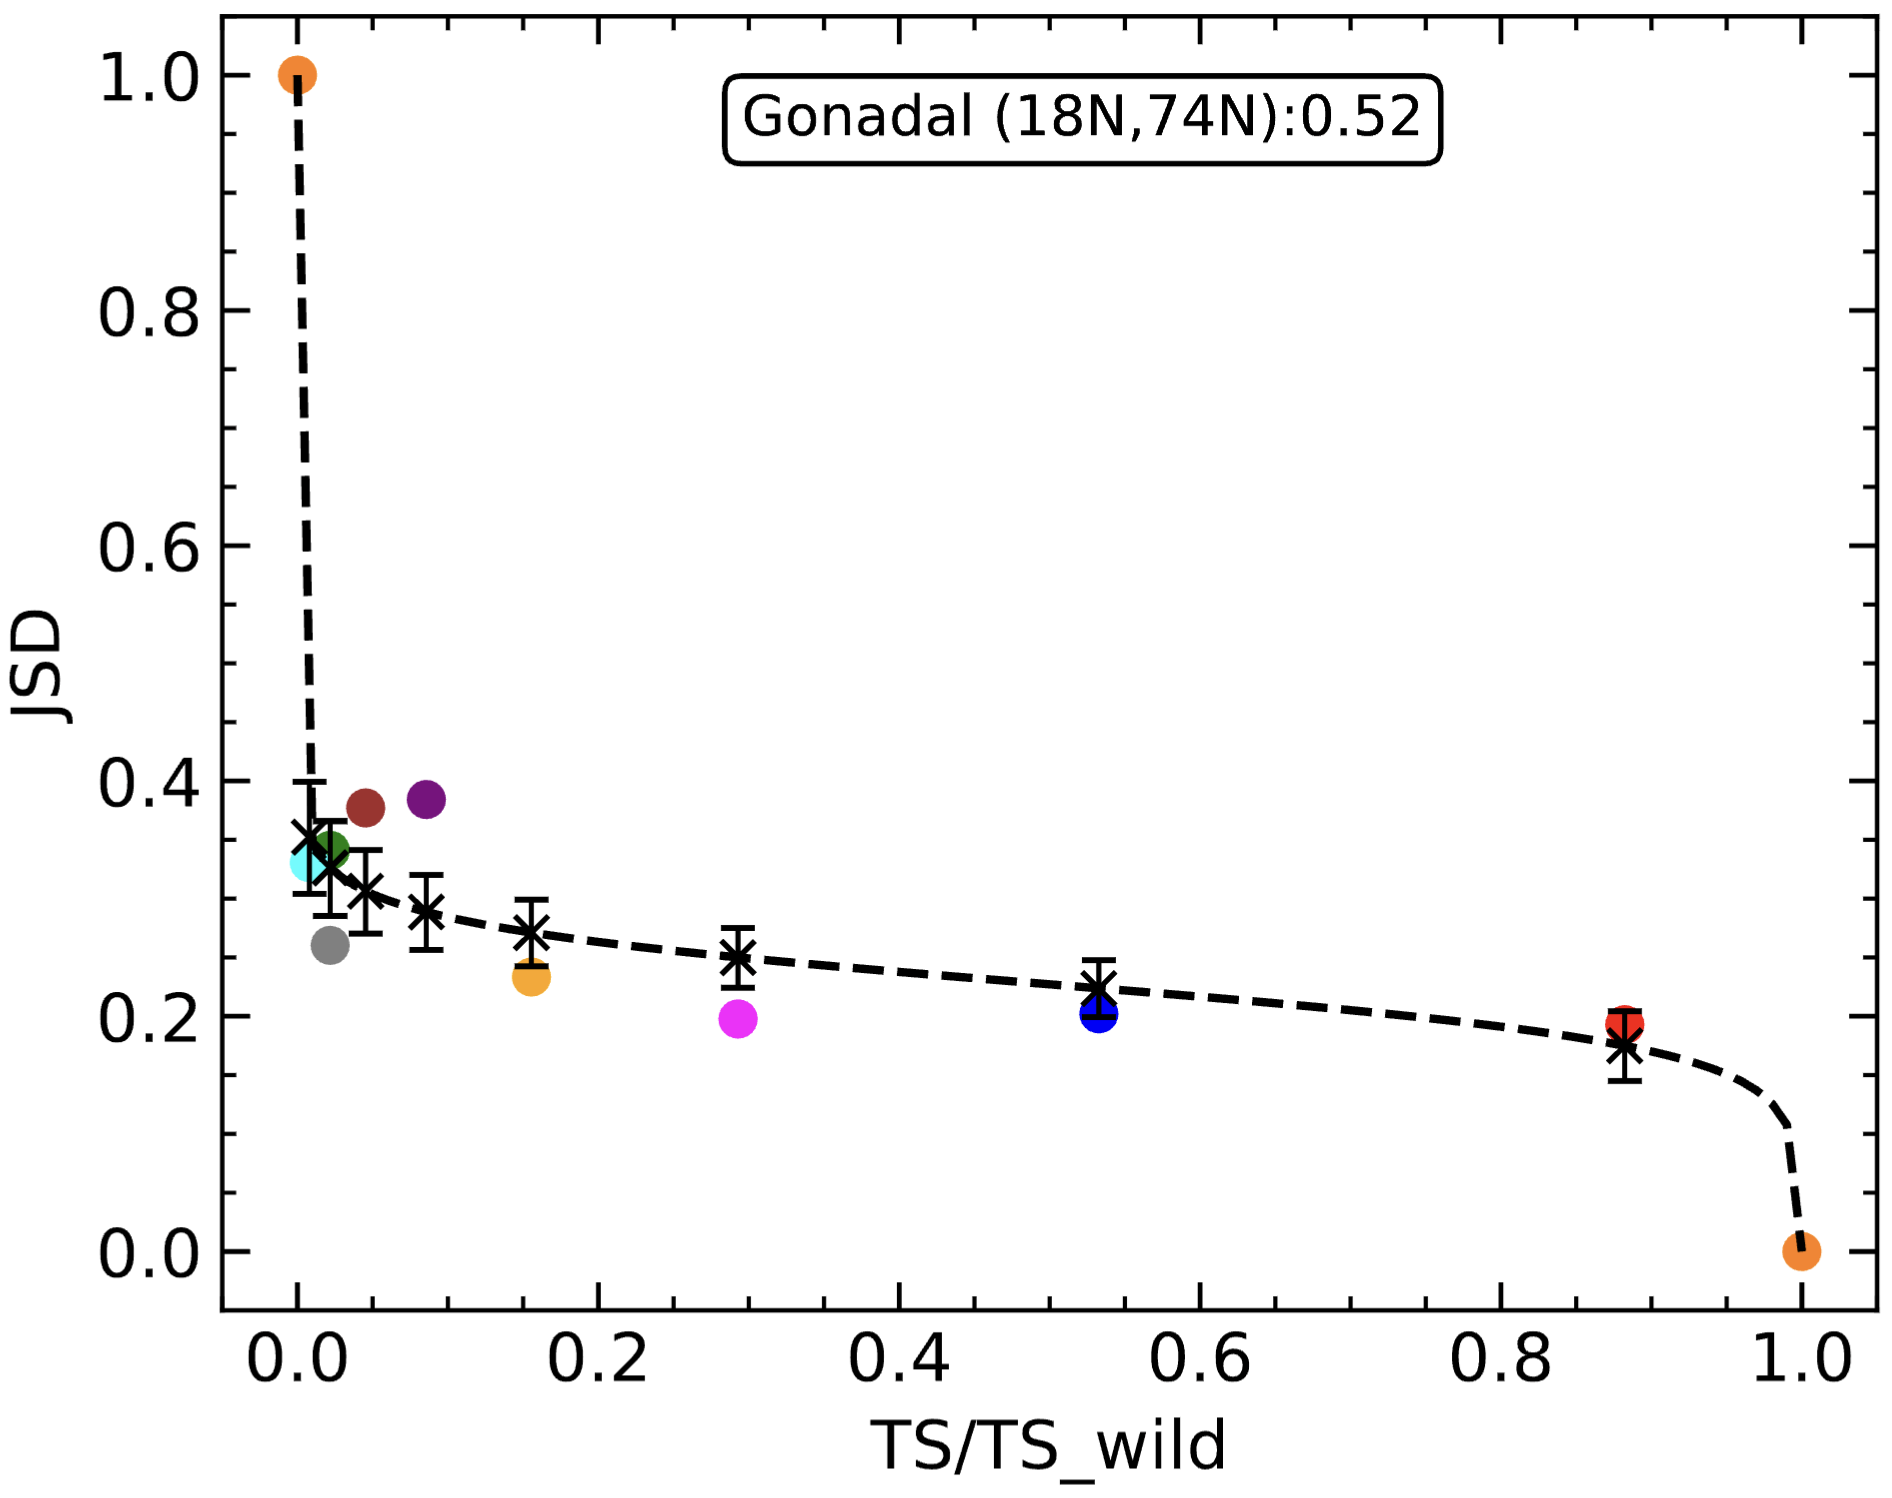
\includegraphics[height=0.4\textwidth]{Abhay_Lakshmi_old/Results/jsd_ts_net_bio_fig.png}} &
% 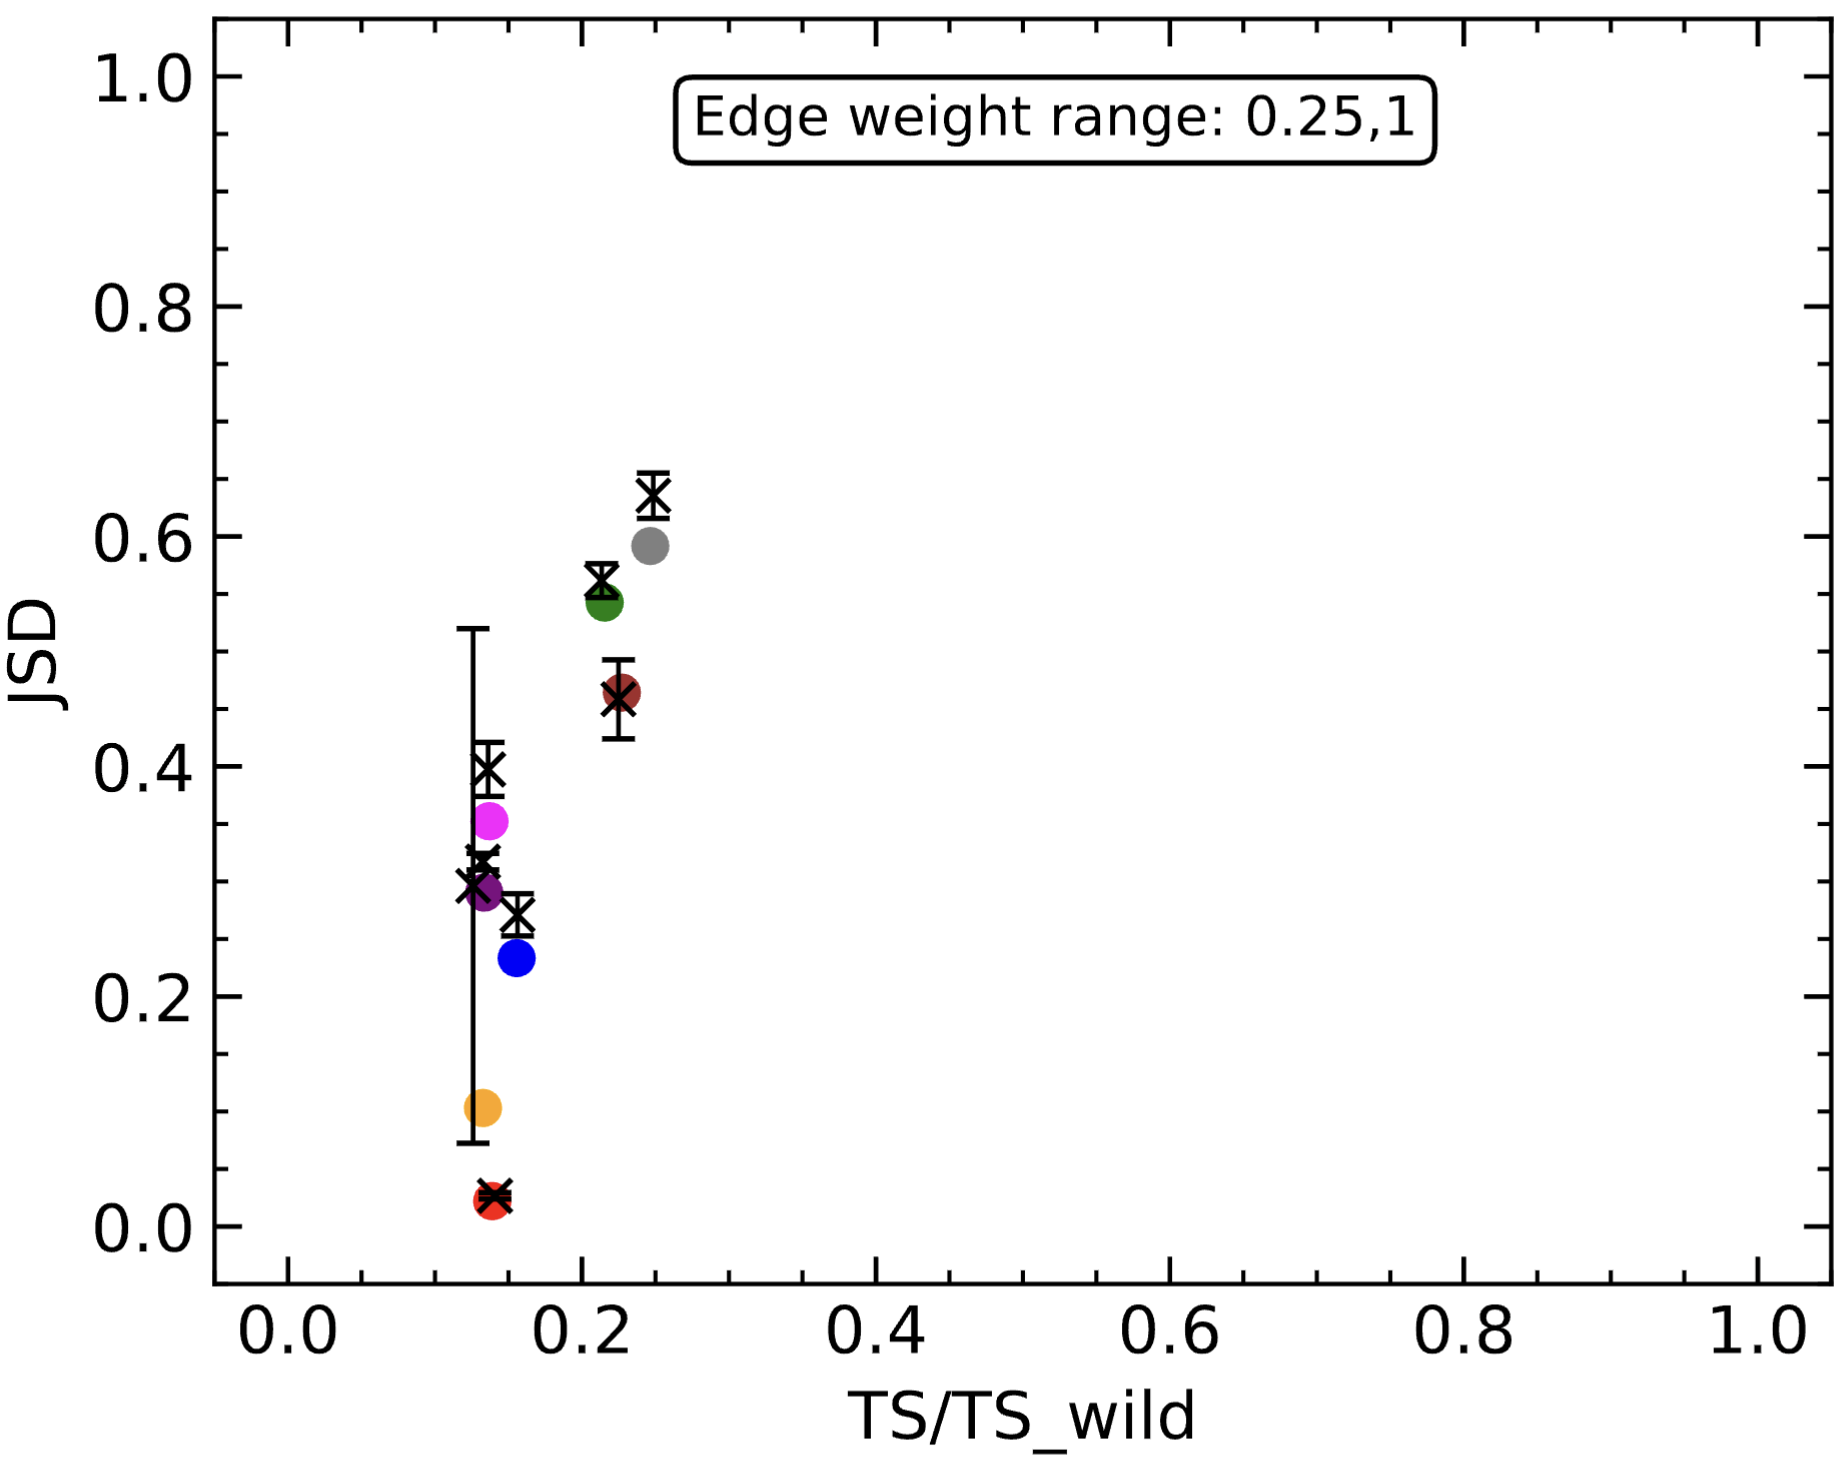
\includegraphics[height=0.4\textwidth]{Abhay_Lakshmi_old/Results/jsd_ts_ew_bio_fig.png} &
% {\raisebox{0.8cm}{\hspace{-0.15cm}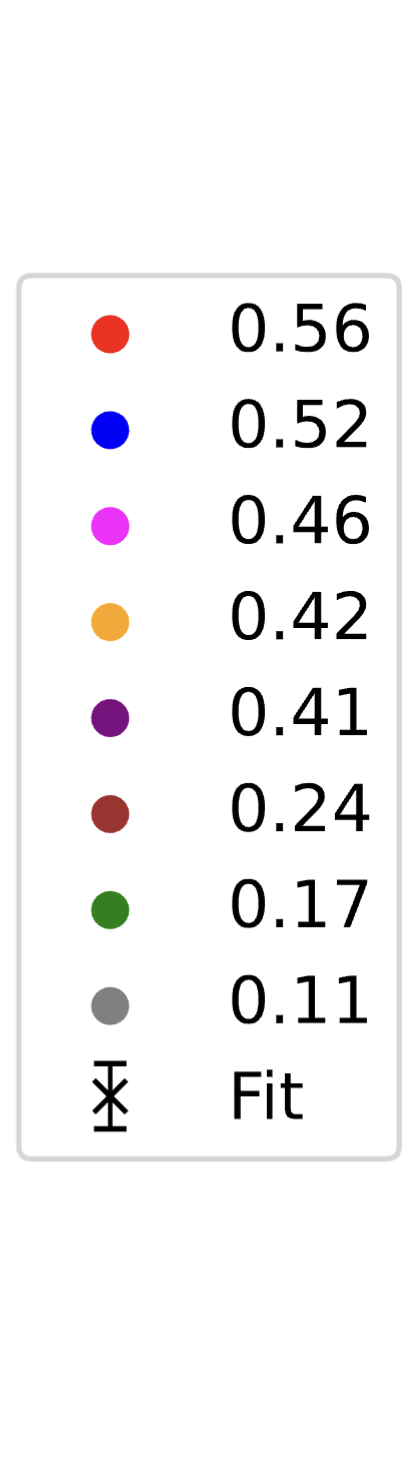
\includegraphics[height=0.3\textwidth]{Abhay_Lakshmi_old/Results/jsd_ts_ew_bio.png}}}

% \end{tabular}
% }
% \caption{
% \textbf{Quantification $\jsd$ as a function of $\ts/\tsw$ for static edge-weight perturbations}: Unless mentioned otherwise, the network along with its nodes, edges, and wild-type team strength is shown in the title. \textit{Top:} (right) Quantification of the mean of team-strength distributions ($\ts$) normalized by the corresponding wild-type team strength ($\tsw$), $\ts/\tsw$, as a function of the edge-weight noise levels ($\ewnum$; numerical values of the edge-weight noise ranges; see \S\ref{tt:ew_range_num}) using Eq.~\ref{eq:ts_ewnum} (black-dashed line) displayed along with the error bars (see Tab.~\ref{tab:ew_param}) for $\tsten$. (left) JSD distributions for edge-weight noise ranges along with their mean ($\jsd$) (green square) and median (orange line) for $\tseight$. \textit{Middle:} (right) Quantification $\jsd$ as a function of $\ts/\tsw$ for a given artificial network: Plot of $\jsd$ and $\ts/\tsw$ across edge-weight noise ranges (legend; left) along with their fit of the Eq.~\ref{eq:jsd_ts_net} (black-dashed line; see Tab.~\ref{tab:ew_param}) for $\tseight$; For an artificial network, the resilience of steady-state distribution increases with an increase in the strength of teaming interactions. (left) $\jsd$ vs. $\ts/\tsw$ for a given edge-weight noise level (in terms of range; here $[0.75,1]$; see title) across networks (represented in terms of their wild-type team strength $\tsw$; see legend); The data in black are $\jsd$ and their error bars obtained from Eq.~\ref{eq:jsd_ts_ran} with no fitting; For a static edge-weight noise level, the resilience increases with an increase in team strength across artificial networks. \textit{Bottom:} The plots represent the same as the middle panels except for biological networks. To rule out over-fitting, we have tested our models for the edge-weight noise range $[0.2,0.3]$ (see legend of left panel). The contrast is in the right panel where $\jsd$ increases with increasing $\ts/\tsw$; This observation remains to be explained.
% }
% \label{fig:S2}
% \end{figure*} 



%%%%%%%%%%%%%%%%%%%%%%%%%%%%%%%%%%%%%%%%%%%%%%%%%%%%%%%%%%%%
%%% APPENDICES
%%%%%%%%%%%%%%%%%%%%%%%%%%%%%%%%%%%%%%%%%%%%%%%%%%%%%%%%%%%%
% \newpage
% \begingroup
% \setlength{\tabcolsep}{0.7pt} % 
% \renewcommand{\arraystretch}{1.5}
% \begin{table}
% 	\caption{Fitted parameters for Equation \ref{eq:jsd_ts_ran}}
% 	\label{tab:ew_param}
% \begin{threeparttable}
% \begin{tabular}{l|c|lll|ll}
% \hline
% \hline
% \multicolumn{1}{c|}{Network} & \multicolumn{1}{c|}{$\ts_\mathrm{wild}$} & \multicolumn{3}{c|}{$\ts$ parameters} & \multicolumn{2}{c}{$\jsd$ Parameters}\\
% \hline
% \hline
% \multicolumn{1}{c|}{} & \multicolumn{1}{c|}{} & \multicolumn{1}{c|}{$p$} & \multicolumn{1}{c|}{$q$}  & \multicolumn{1}{c|}{$r$} & \multicolumn{1}{c|}{$a$} & \multicolumn{1}{c}{$b$}\\
% \multicolumn{1}{c|}{(1)} & \multicolumn{1}{c|}{(2)} & \multicolumn{1}{c|}{(3)} & \multicolumn{1}{c|}{(4)} & \multicolumn{1}{c|}{(5)} & \multicolumn{1}{c|}{(6)} & \multicolumn{1}{c}{(7)}\\
% \hline
% $\tsten$  & $0.90$ & $(8.07\pm0.95)\times10^{-3}$ & $(2.34\pm0.06)\times10^{-1}$  & $(-8.07\pm5.23)\times10^{-3}$ & $(0.00\pm0.00)\times10^{-2}$ & $0.13\pm0.00$\\
% $\tstwo$  & $0.88$ & $(7.39\pm0.87)\times10^{-3}$ & $(2.38\pm0.06)\times10^{-1}$  & $(-5.19\pm4.99)\times10^{-3}$ & $(0.01\pm0.00)\times10^{-2}$ & $0.01\pm0.00$\\
% $\tsfour$ & $0.86$ & $(6.51\pm0.79)\times10^{-3}$ & $(2.45\pm0.06)\times10^{-1}$  & $(-3.59\pm4.80)\times10^{-3}$ & $(0.22\pm0.01)\times10^{-2}$ & $0.01\pm0.00$\\
% $\tssix$  & $0.82$ & $(4.67\pm0.52)\times10^{-3}$ & $(2.61\pm0.06)\times10^{-1}$  & $(-3.09\pm3.81)\times10^{-3}$ & $(1.36\pm0.31)\times10^{-2}$ & $0.05\pm0.01$\\
% $\tseight$& $0.61$ & $(2.84\pm0.01)\times10^{-3}$ & $(2.86\pm0.01)\times10^{-1}$  & $(-0.38\pm0.64)\times10^{-3}$ & $(0.89\pm0.26)\times10^{-2}$ & $0.25\pm0.01$\\
% \hline
% \hline
% \end{tabular}
% \end{threeparttable}
% \end{table}
% \endgroup
% \newpage


% \section{Appendix}

% \section{Evaluating the effect of additive noise against the corresponding stationary distribution}

% Additive noise leads to an increase in node expression, increasing the residence time of hybrid states ((1,1) state in toggle switch). Among the three noises tested, additive noise also has the highest variance, with a high chance of achieving $\lambda \approx 1$ - weakening the inhibitions in the toggle switch and potentially allowing the nodes to express independently. Thus, it is important to understand if increasing hybrid state MRT is due to the distribution of $\lambda$s created by the additive noise or if the noise itself is required. We thus perfomed experiments to answer the following questions

% \begin{enumerate}

%     \item Do deterministic simulations of the toggle switch parameters with $\lambda$ sampled from the distributions generated by additive noise lead to an increase in the MRT of (1, 1) state?
%     \item Does modifying the noise to ensure lambda switching between 0.01 and 1 (instead of increments by normal random variable) increase the frequency of the (1, 1) state?
% \end{enumerate}
% The original formulation of additive noise follows the equation below:

% \begin{equation}
% \begin{split}
%     \lambda(t+1) &\overset{\text{Additive}}{=} 
%         \lambda(t) + \mathcal{N}(0,\sigma)\\
%     \lambda(t+1) &= \text{clip}\bigl(\lambda(t+1),\ 0.01,\ 1\bigr)
% \end{split}
% \label{additiveNoise}
% \end{equation}

% We devised two additional forms of noise - named the Jumping noise and the Extreme noise - defined as follows:


% % \centering
% \begin{equation}
% \begin{split}
%     \lambda(t+1) &\overset{\text{Jumping}}{=} 
%     \begin{cases}
%         \lambda(t) + \sigma & \text{if } \mathcal{N}(0,\sigma) > 0 \\
%         \lambda(t) - \sigma & \text{if } \mathcal{N}(0,\sigma) < 0
%     \end{cases} \\[6pt]
%     \lambda(t+1) &= \text{clip}\bigl(\lambda(t+1),\ 0.01,\ 1\bigr)
% \end{split}
% \label{jumpingNoise}
% \end{equation}

% \begin{equation}
%     \lambda (t+1) \overset{Extreme}{=} \begin{cases}
%         1 \ if \ N(0,\sigma) > 0\\
%         0.01 \ if \ N(0,\sigma) < 0
%     \end{cases}
%     \label{extremeNoise}
% \end{equation}



% We then derived the distribution of $\lambda$ for five values of $\sigma$ : ${0.001, 0.005, 0.01, 0.05, 0.1}$ numerically and simulated toggle switch as follows:

% \begin{itemize}
%     \item Sample a subset of models $\{m_i\}$ from RACIPE and extract the $\lambda$ values
%     \item For each such $\lambda$, run 100 trajectories of $\lambda$, using the corresponding noise equation (Eq \ref{additiveNoise}, \ref{jumpingNoise}, \ref{extremeNoise}), for 10000 time steps.
%     \item Collect the values of $\lambda$ from all the 100 trajectories to use as the distribution for the corresponding noise type. 
%     \item Generate 10 new models $\{m_{i_j}\}$, each model having the same parameters as the original RACIPE model, except for the $\lambda$ values sampled from the distribution generated in the previous step.
%     \item Generate deterministic trajectories for each model starting from 100 randomly generated initial conditions sampled uniformly from the range $[0, \frac{g_A}{k_A}]$, where $g_A$ is the production rate of node $A$ and $k_A$ is the degradation rate. Run each simulation for 10000 time steps
%     \item Discretize each state along these simulations using the threshold values obtained from RACIPE. 
%     \item Evaluate the mean fraction of occurance of each discrete state across all simulations and the 10 models.
%     \item Parallely run stochastic simulations on the original models of RACIPE $\{m_i\}$, starting from the steady states obtained from RACIPE, with $\lambda$ being updated at each time point according to Eq \ref{additiveNoise}, \ref{jumpingNoise}, \ref{extremeNoise}. Evaluate mean residence times of the discrete states across these stochastic trajectories.
% \end{itemize}

% \subsection{Comparing the MRTs of stochastic and deterministic trajectories}

% \begin{figure}
%     \centering
%     \begin{subfigure}[t]{0.48\linewidth}
%         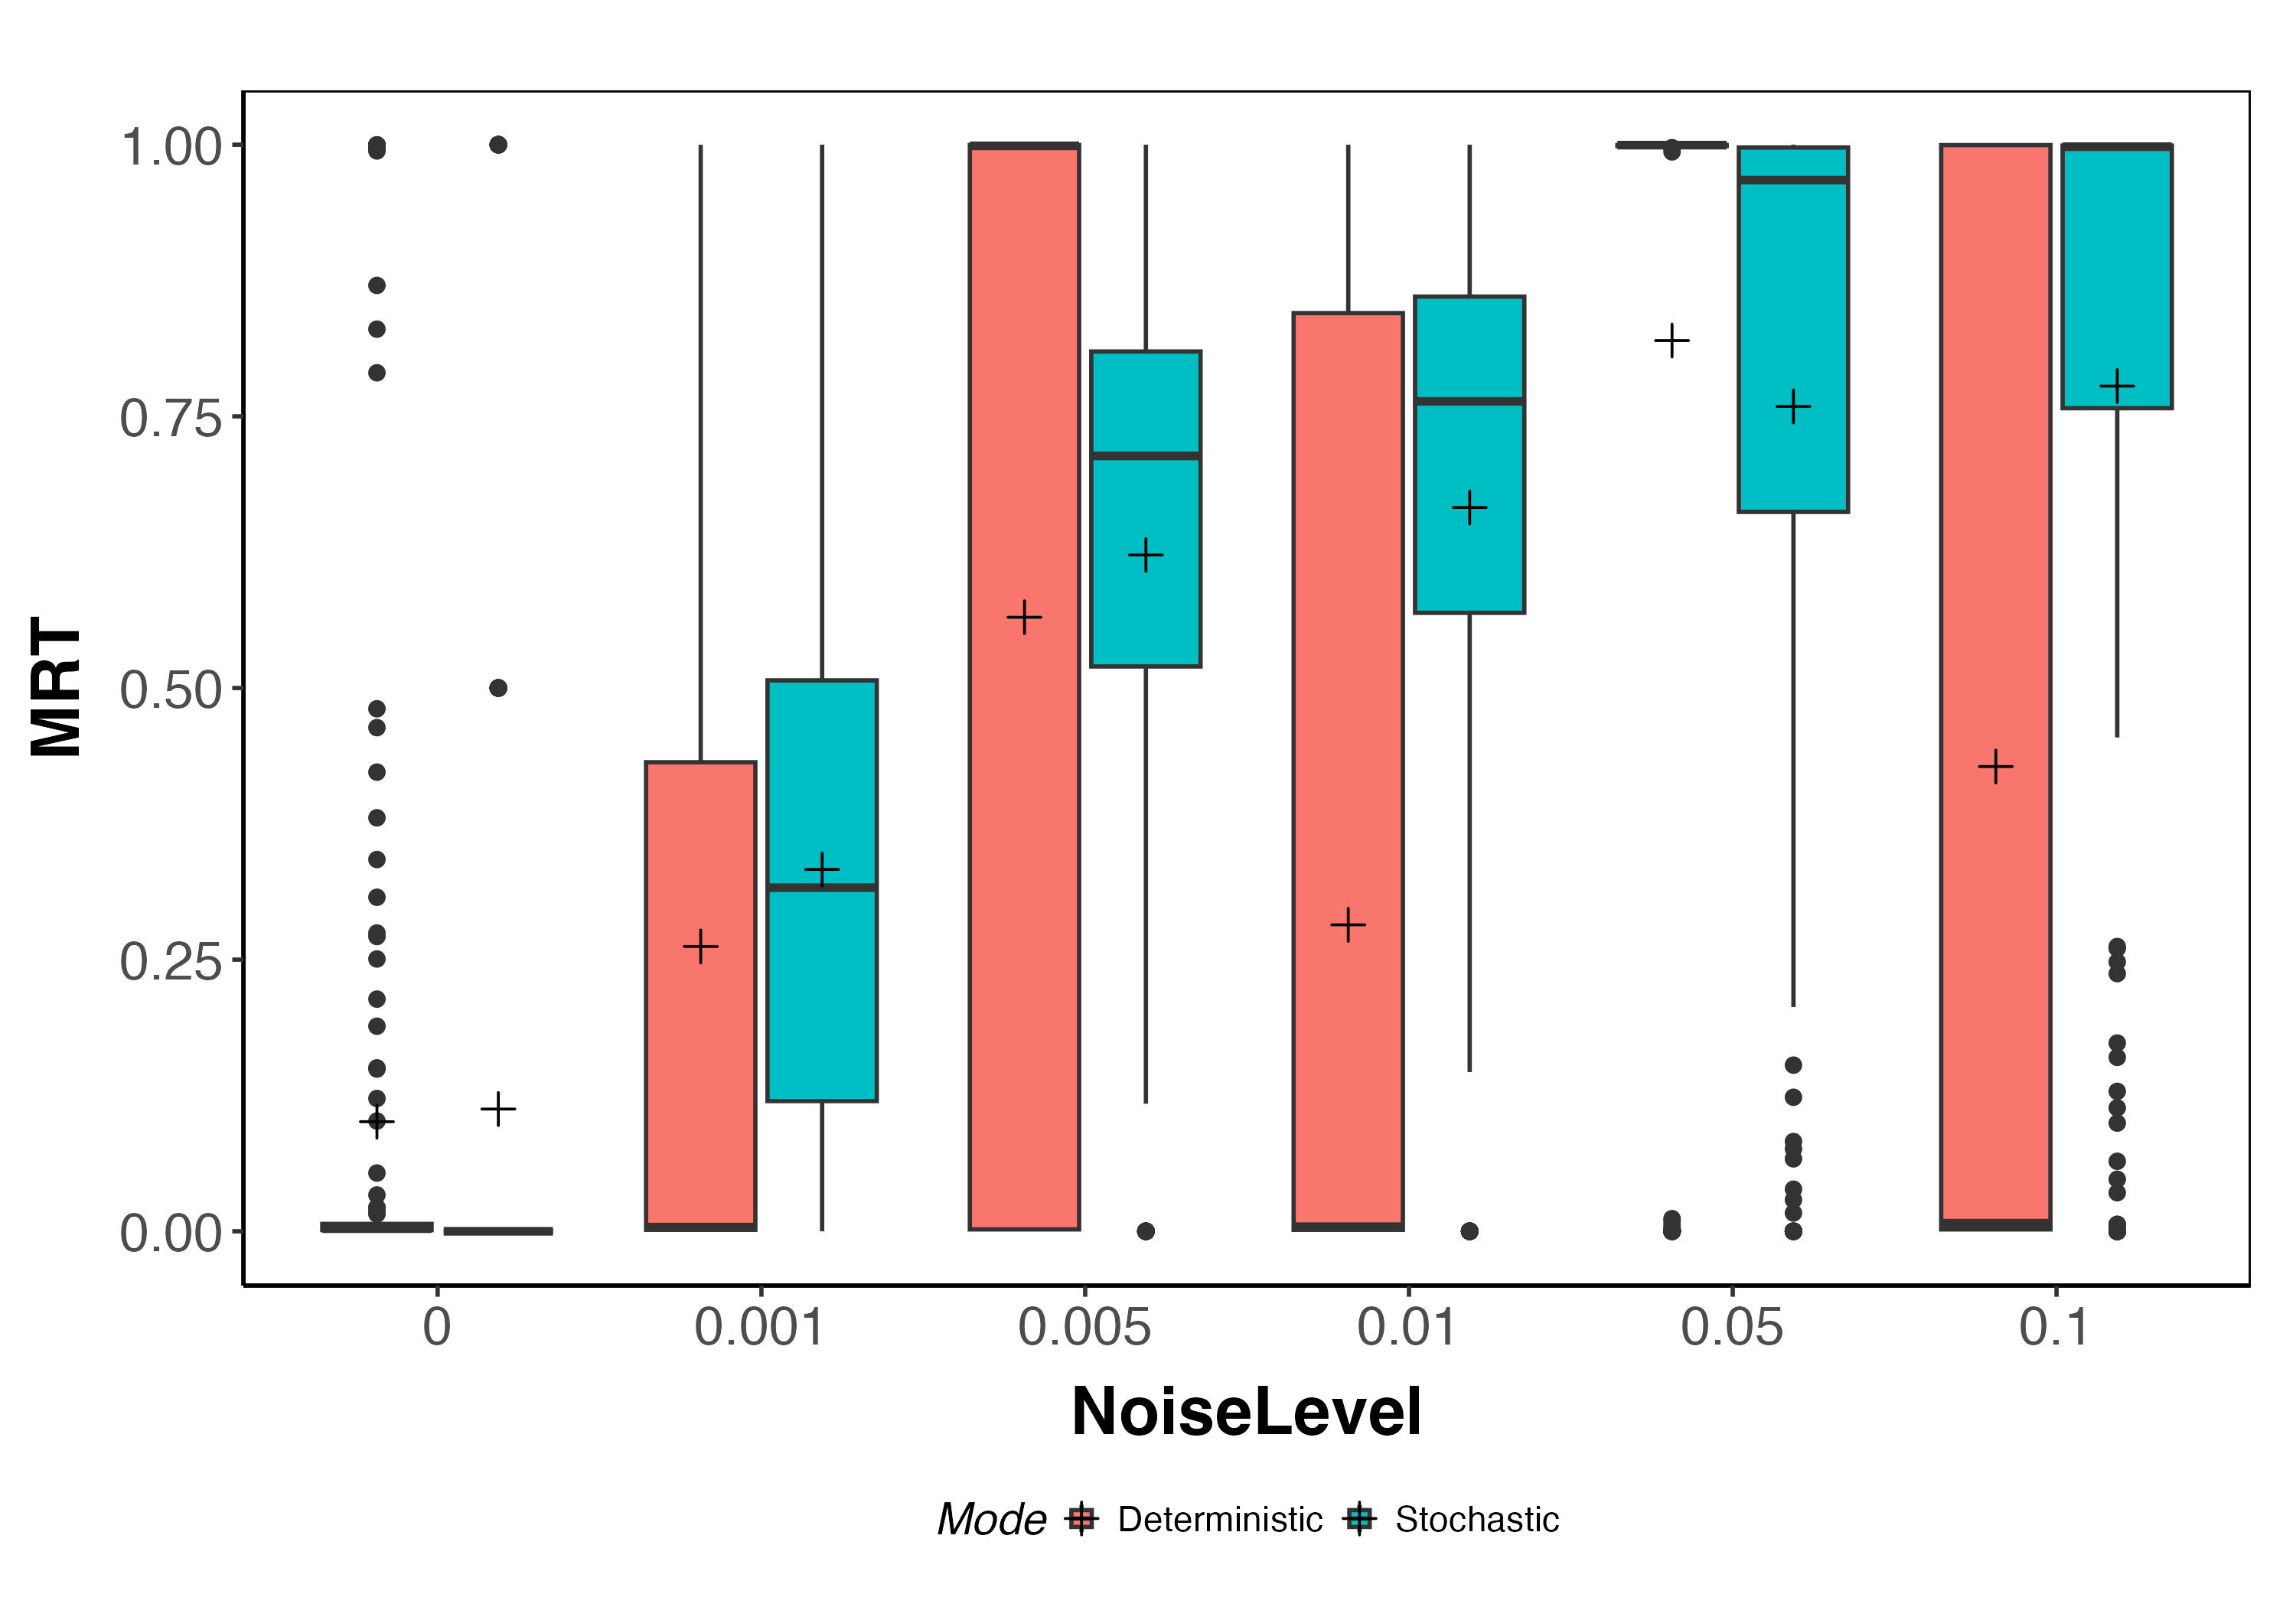
\includegraphics[width=\linewidth]{AditiveNoiseFigures/11Additive.jpg}
%         \caption{Additive noise}
%         \label{fig:additive11}
%     \end{subfigure}
%     \hfill
%     \begin{subfigure}[t]{0.48\linewidth}
%         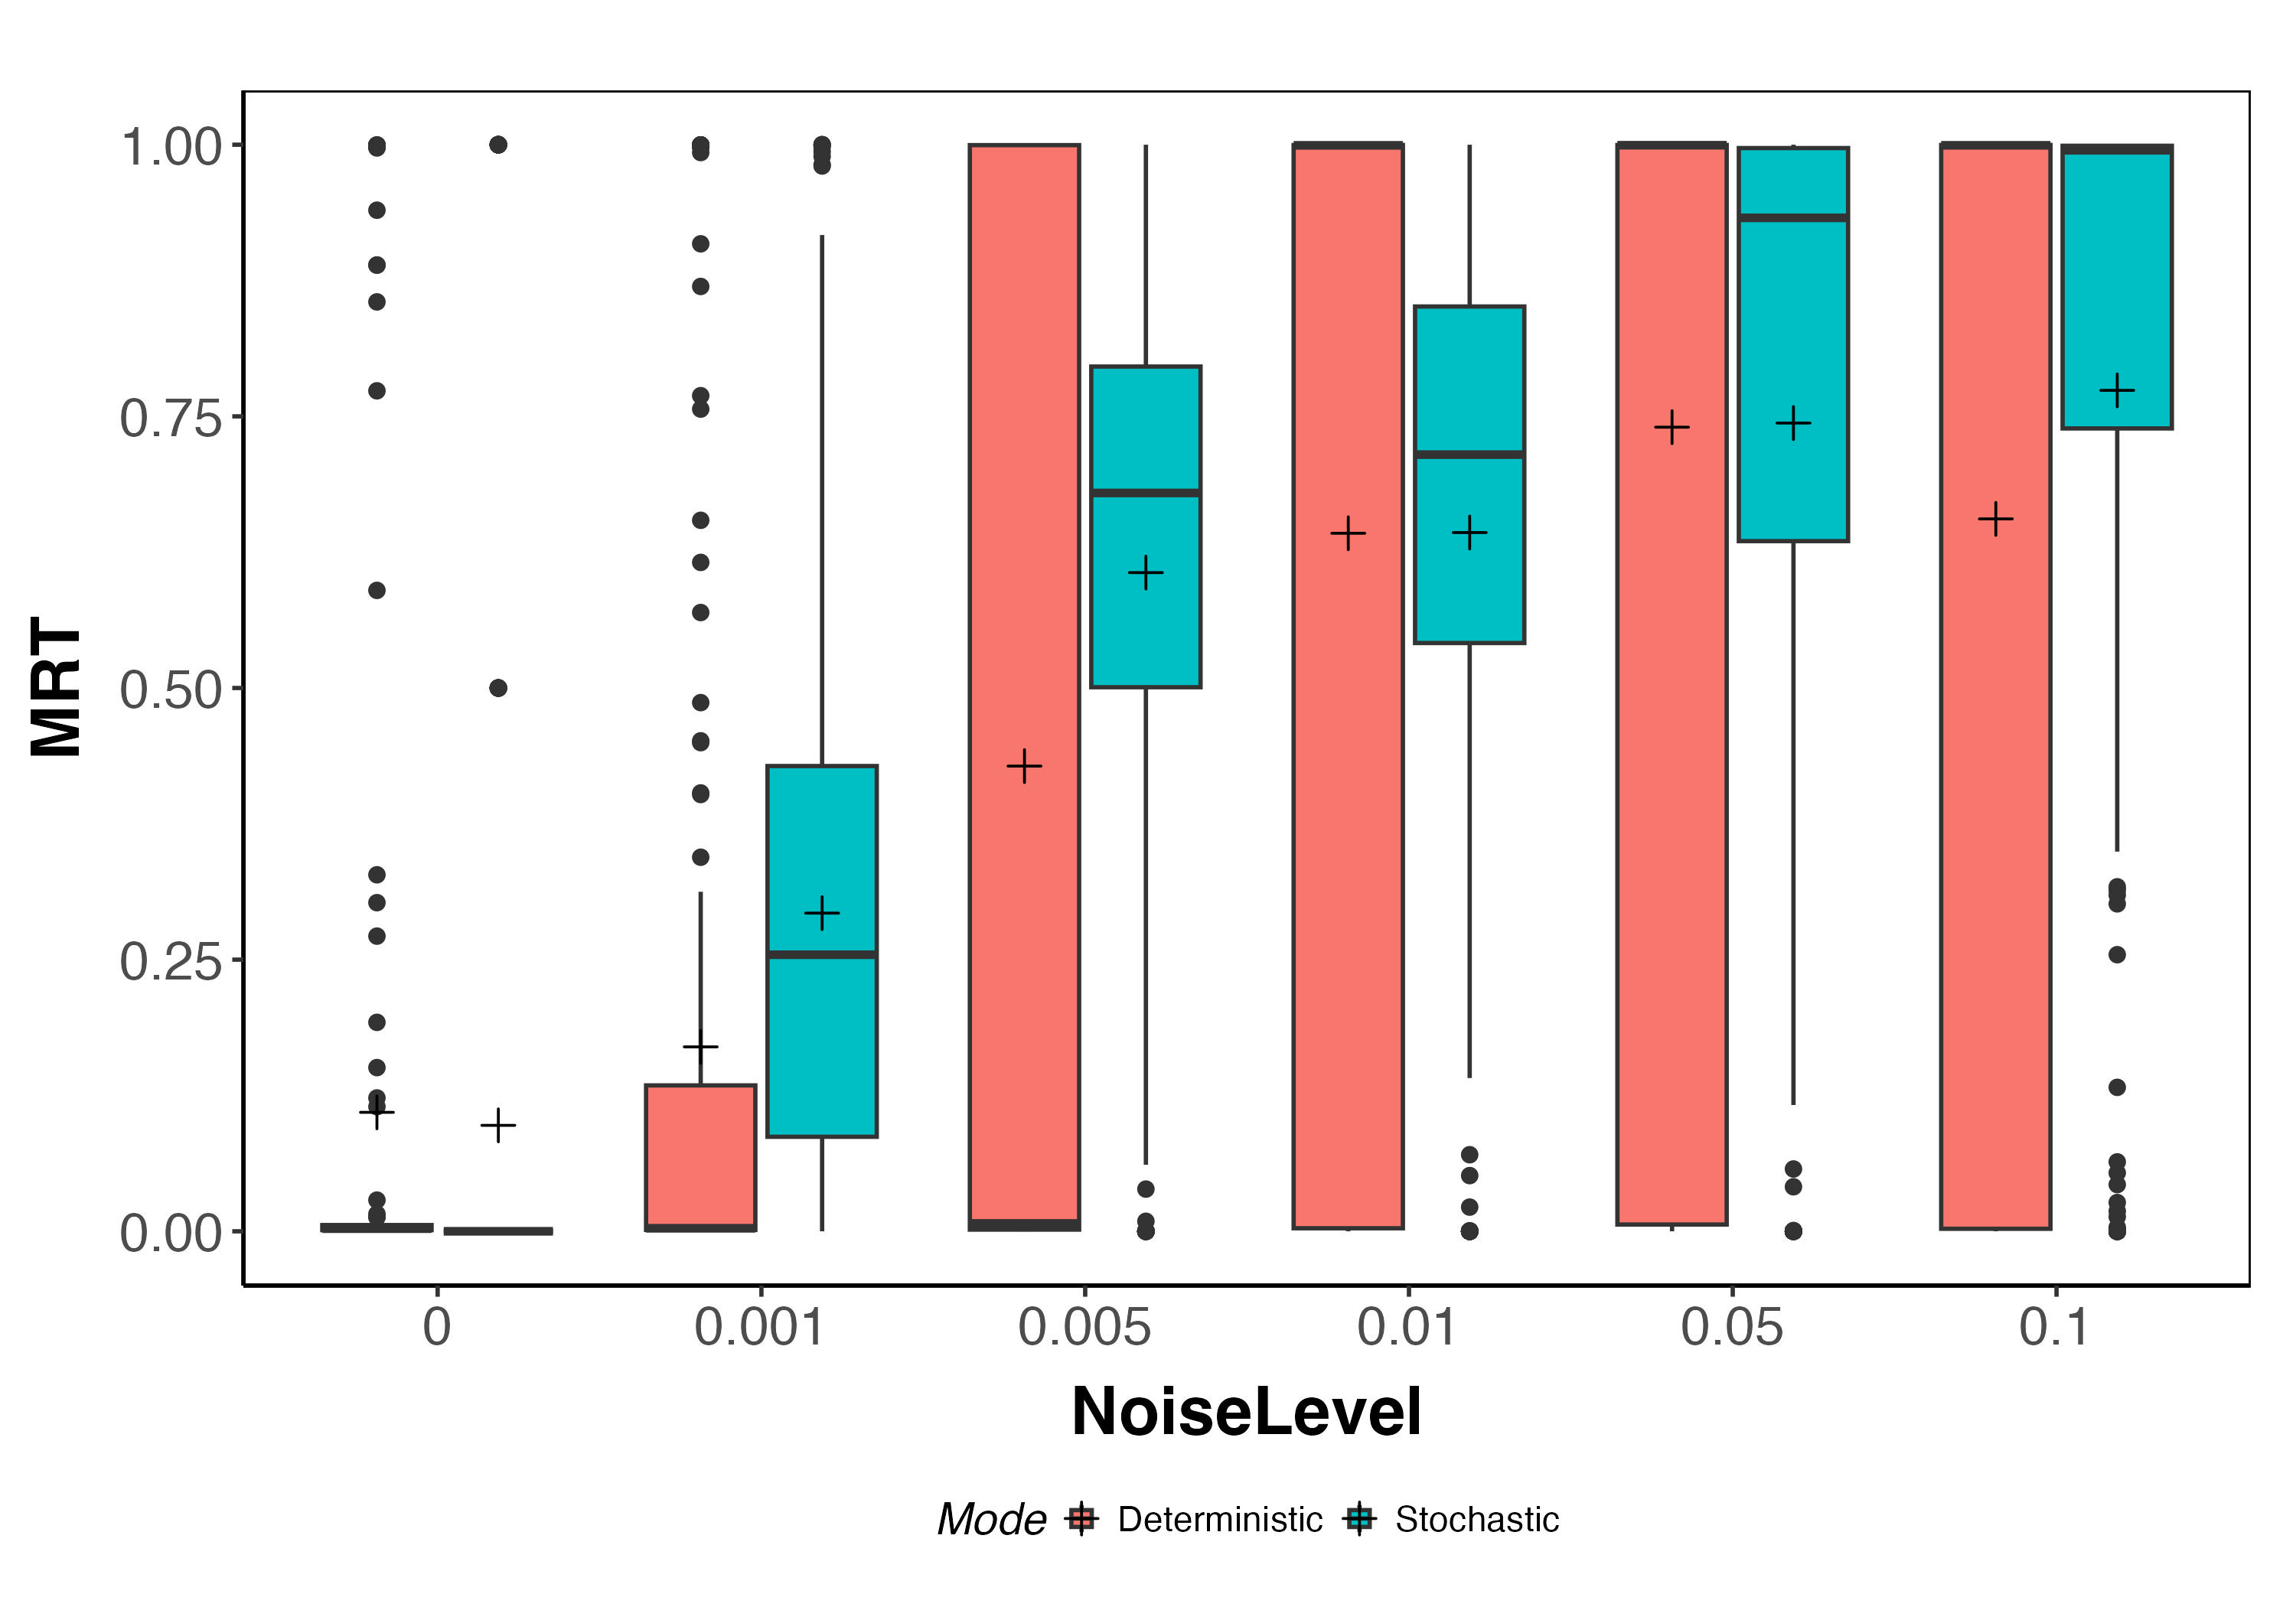
\includegraphics[width=\linewidth]{AditiveNoiseFigures/11Jumping.jpg}
%         \caption{Jumping noise}
%         \label{fig:jumping11}
%     \end{subfigure}

%     \begin{subfigure}[t]{0.48\linewidth}
%         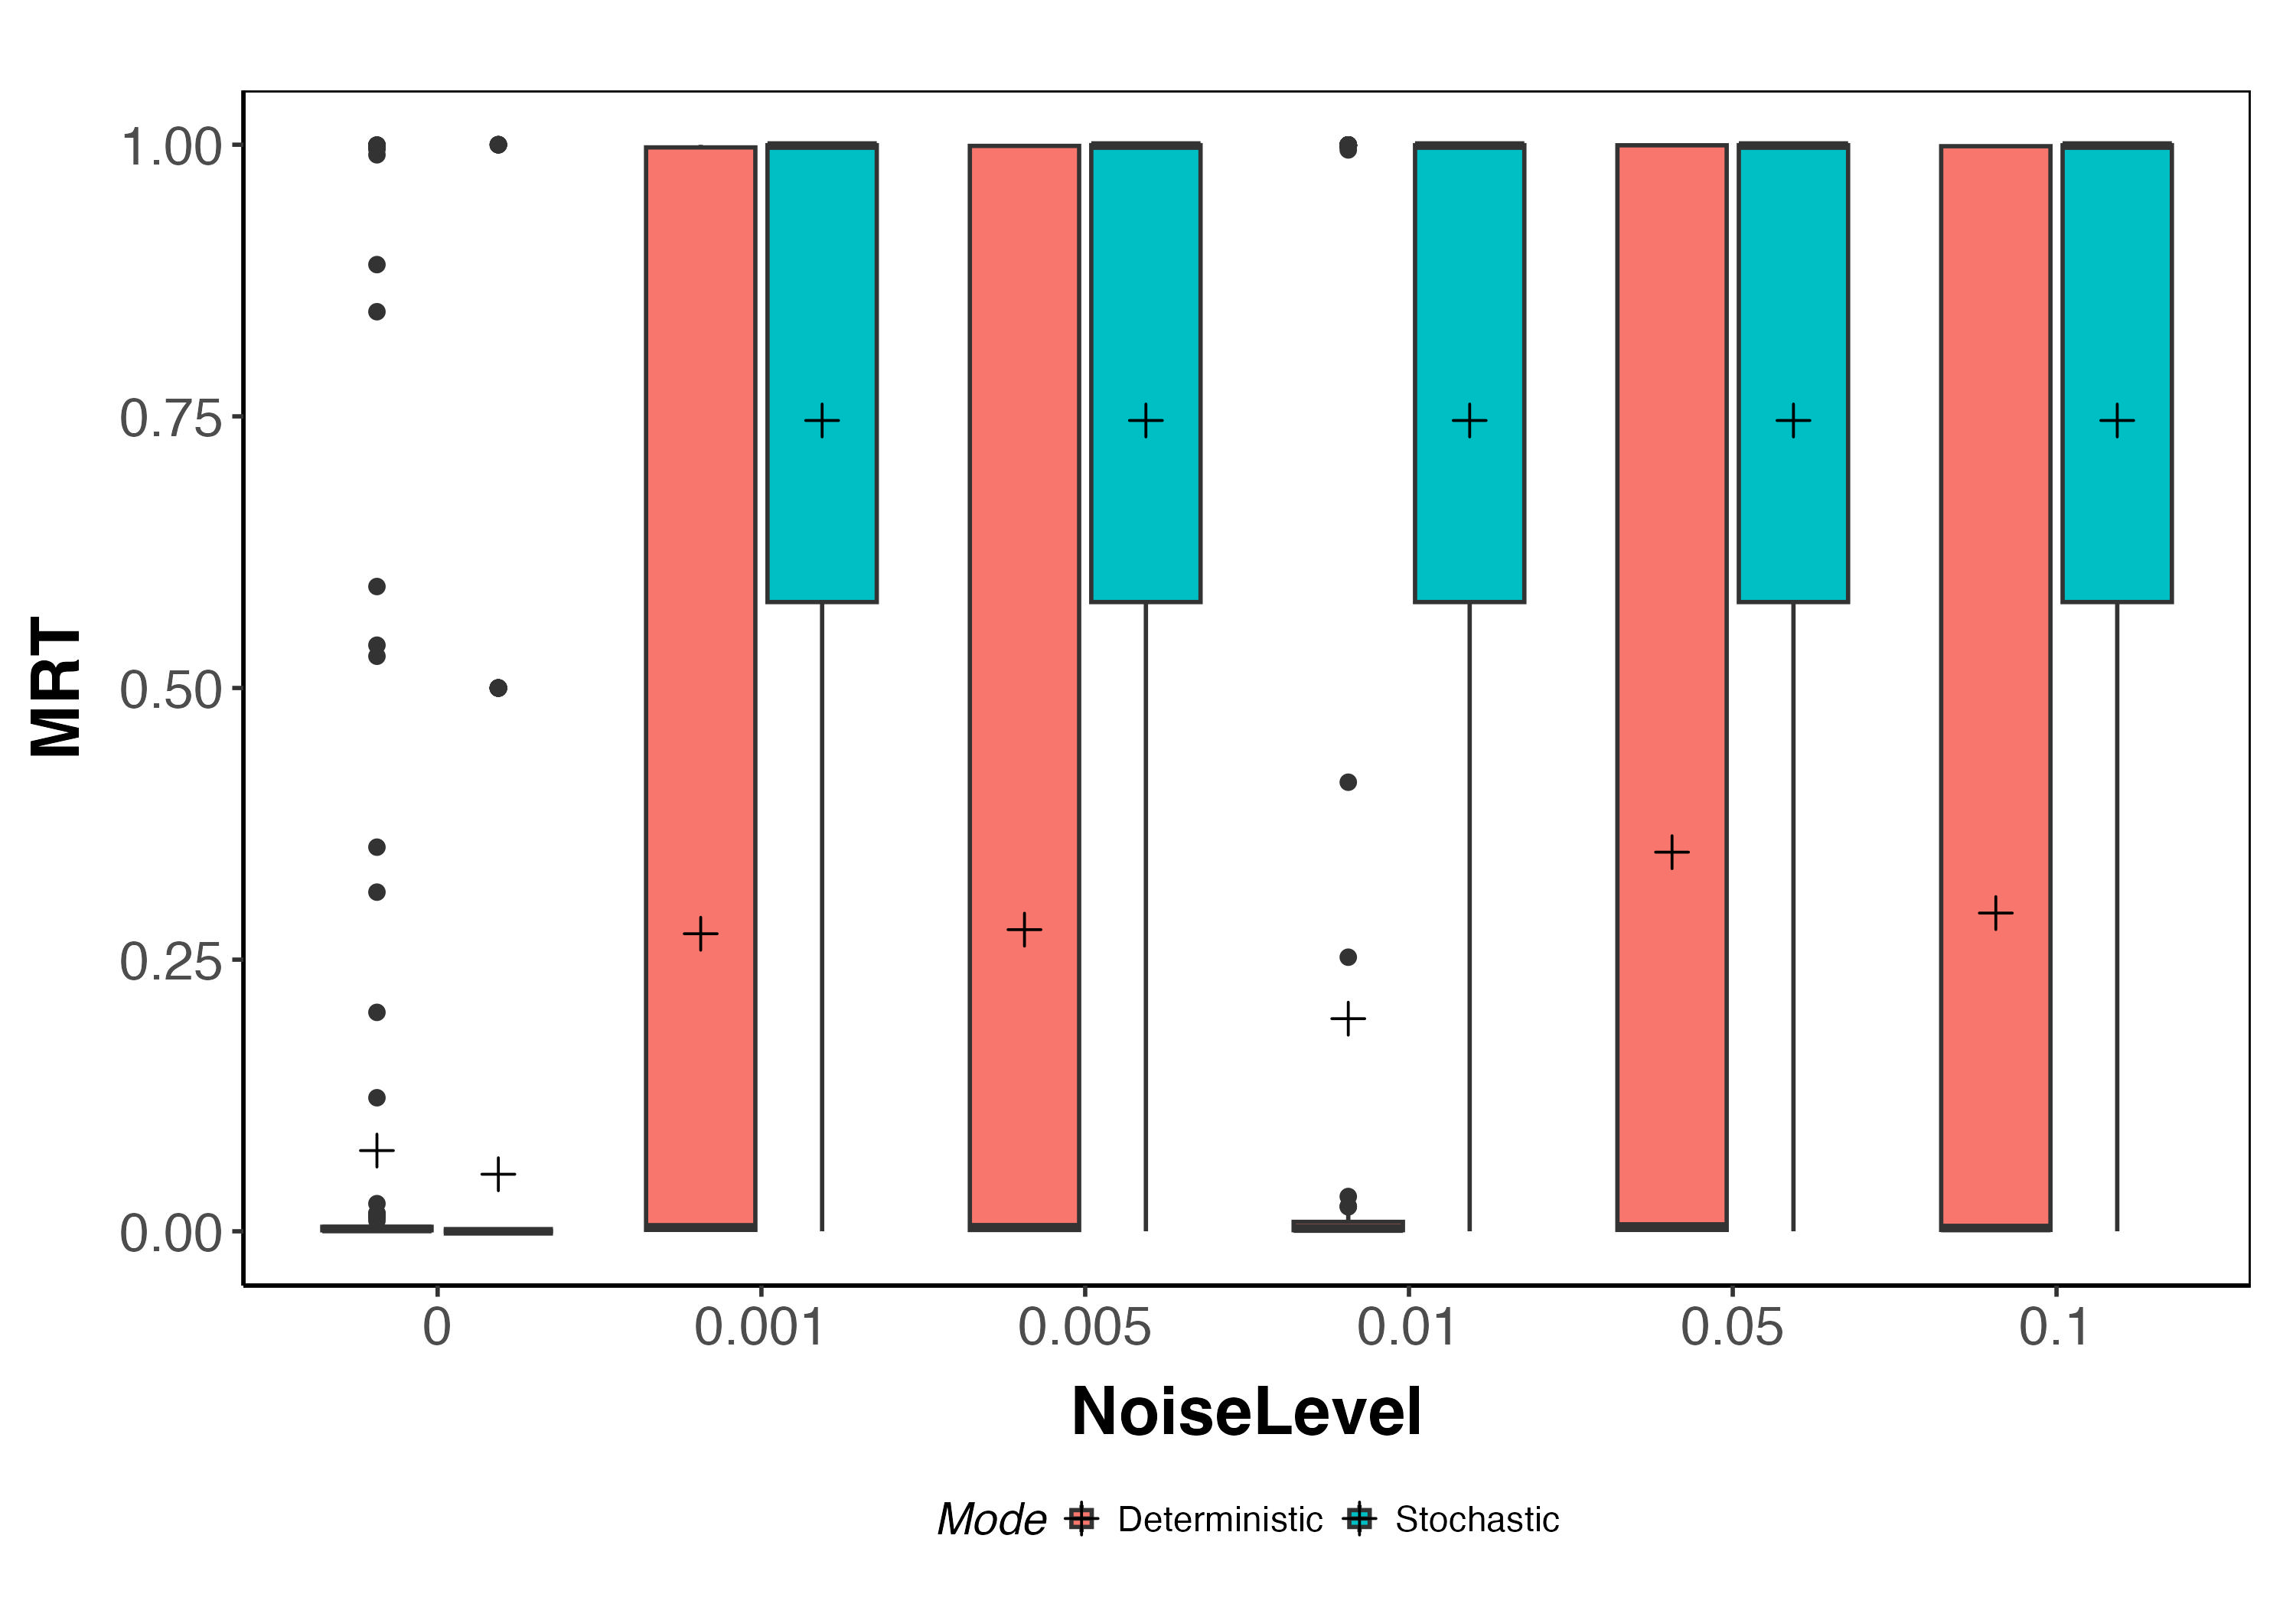
\includegraphics[width=\linewidth]{AditiveNoiseFigures/11Extreme.jpg}
%         \caption{Extreme noise}
%         \label{fig:extreme11}
%     \end{subfigure}
%     \caption{Boxplots showing the comparison of MRTs of the (1,1) state from deterministic (red) and stochastic (green) simulations of Additive, Jumping and Extreme noise. The mean of the each distribution is shown using a '+' symbol, while the median is shown by a black horizontal line segment within each box. The boundaries of the boxes show the IQR.}
%     \label{fig:11MRT}
% \end{figure}

% For both additive and jumping noise, the mean MRT of the (1,1) state is nearly the same for both stochastic and deterministic simulations. Two differences can be highlighted: (1) the median MRT is either 0 or 1 in deterministic simulations irrespective of $\sigma$, whereas the corresponding median for stochastic simulations increases with $\sigma$. (2) The overall distribution for deterministic simulations is extremely bimodal, whereas that for the stochastic simulations shifts to higher values with increasing $\sigma$. These observations suggest that the distribution alone can indeed increase the incidence of (1,1) state in additive noise, but the increase is not consistent. The stochasticity ensures that the MRT of (1,1) remains high. Similar observations can be seen for the jumping noise case. Interestingly, in the case of extreme noise where the $\lambda$ can either be high (1) or low (0.01), the mean MRT in deterministic simulations is always lower than that of stochastic simulations, which could be explained by the fact that given only 4 combinations of $\lambda$ are possible, only one of the combinations can reliably allow the stability of (1,1) state - where both $\lambda$ values are 1. 

% \begin{figure}
%     \centering
%     \begin{subfigure}[t]{0.48\linewidth}
%         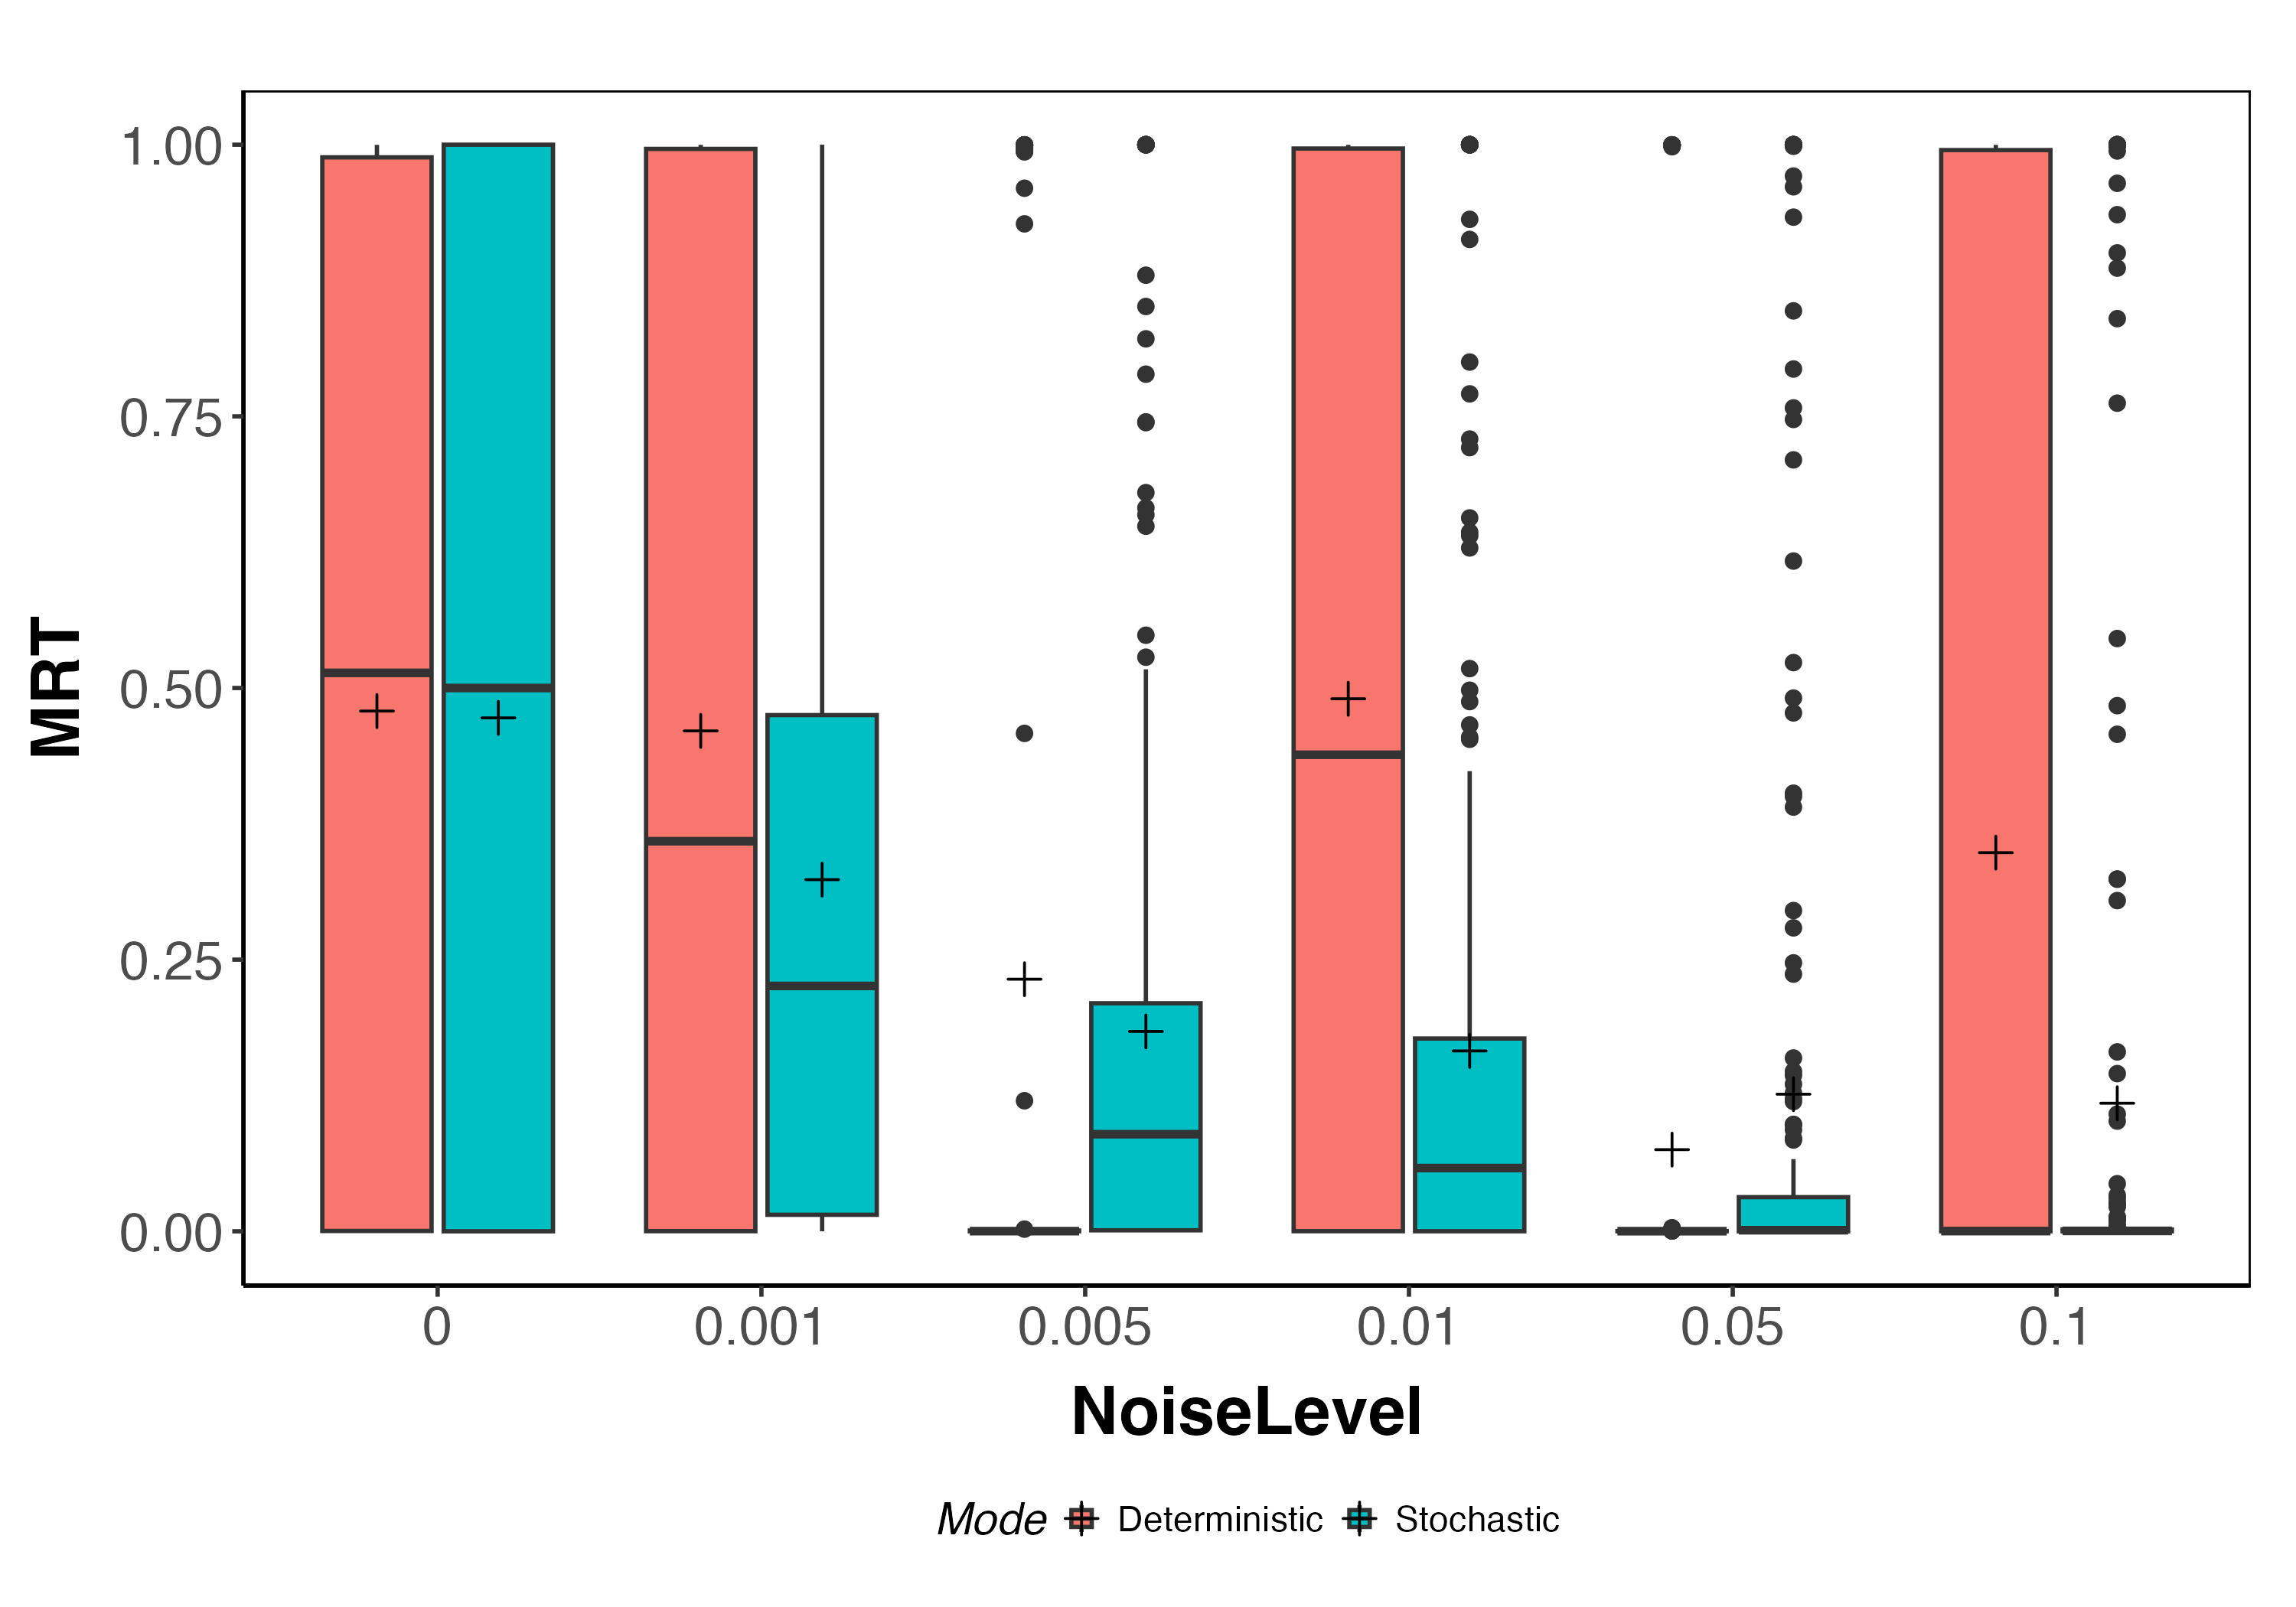
\includegraphics[width=\linewidth]{AditiveNoiseFigures/01Additive.jpg}
%         \caption{Additive noise}
%         \label{fig:additive01}
%     \end{subfigure}
%     \hfill
%     \begin{subfigure}[t]{0.48\linewidth}
%         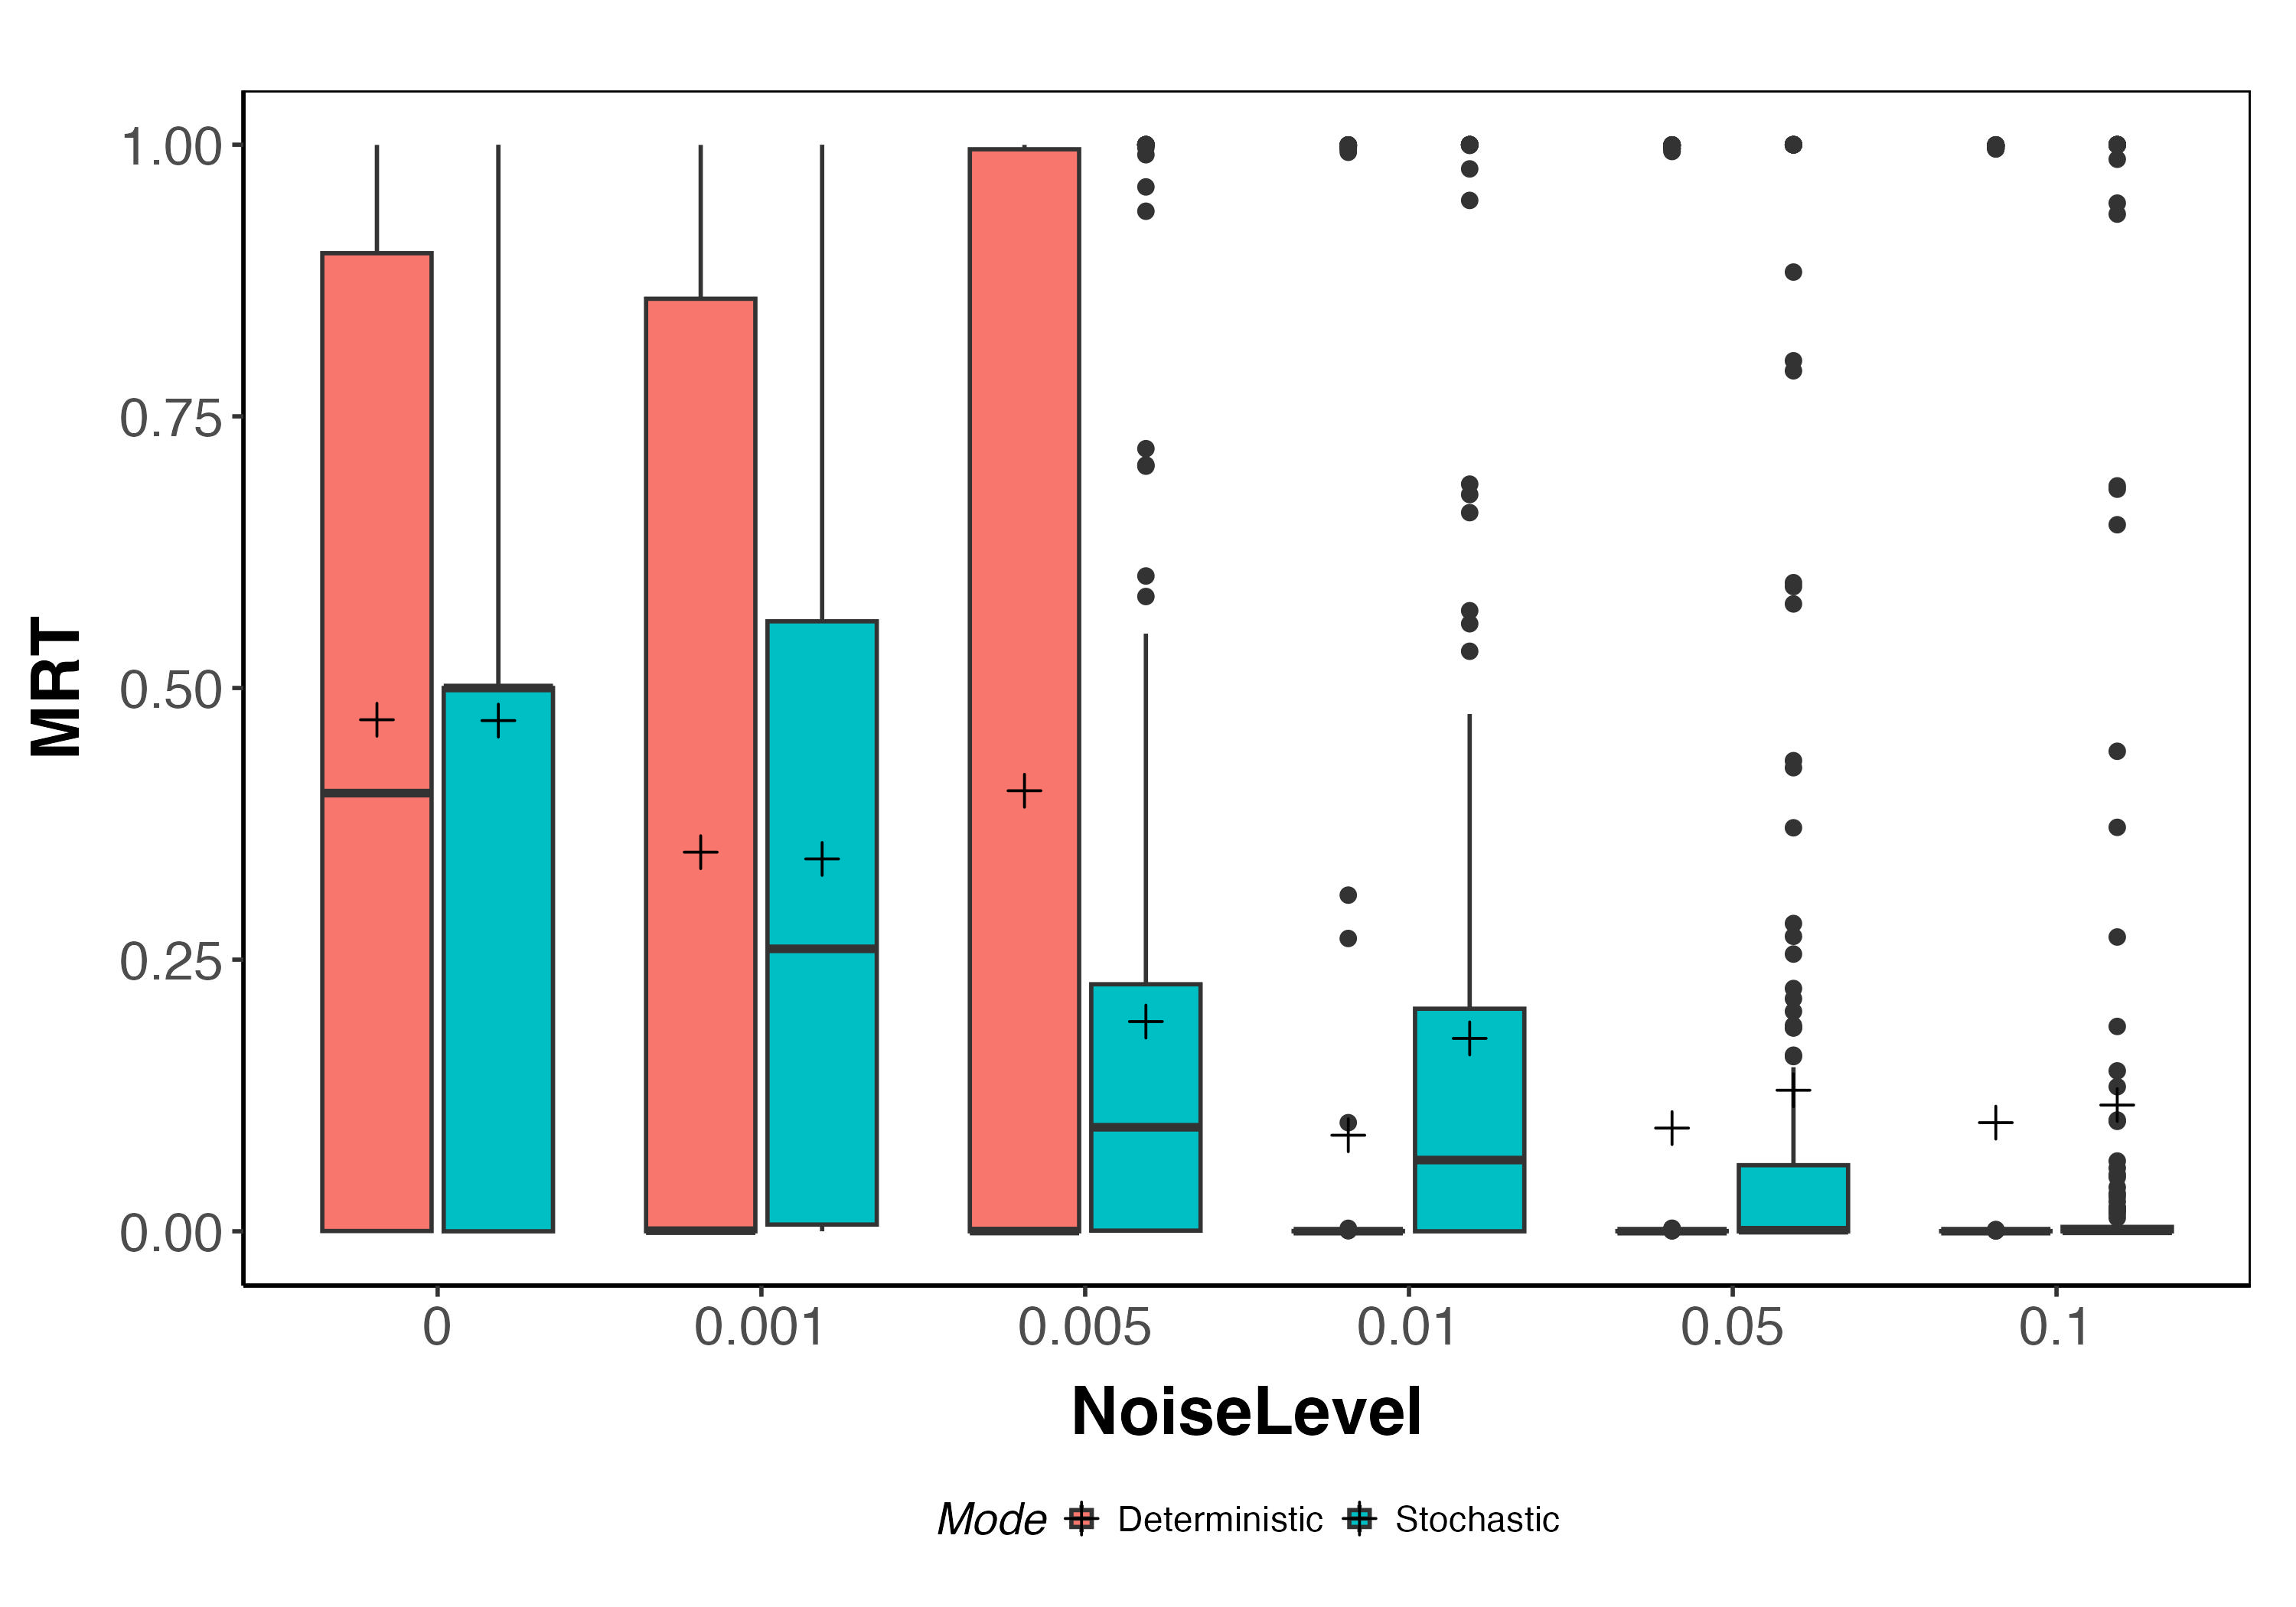
\includegraphics[width=\linewidth]{AditiveNoiseFigures/01Jumping.jpg}
%         \caption{Jumping noise}
%         \label{fig:jumping01}
%     \end{subfigure}

%     \begin{subfigure}[t]{0.48\linewidth}
%         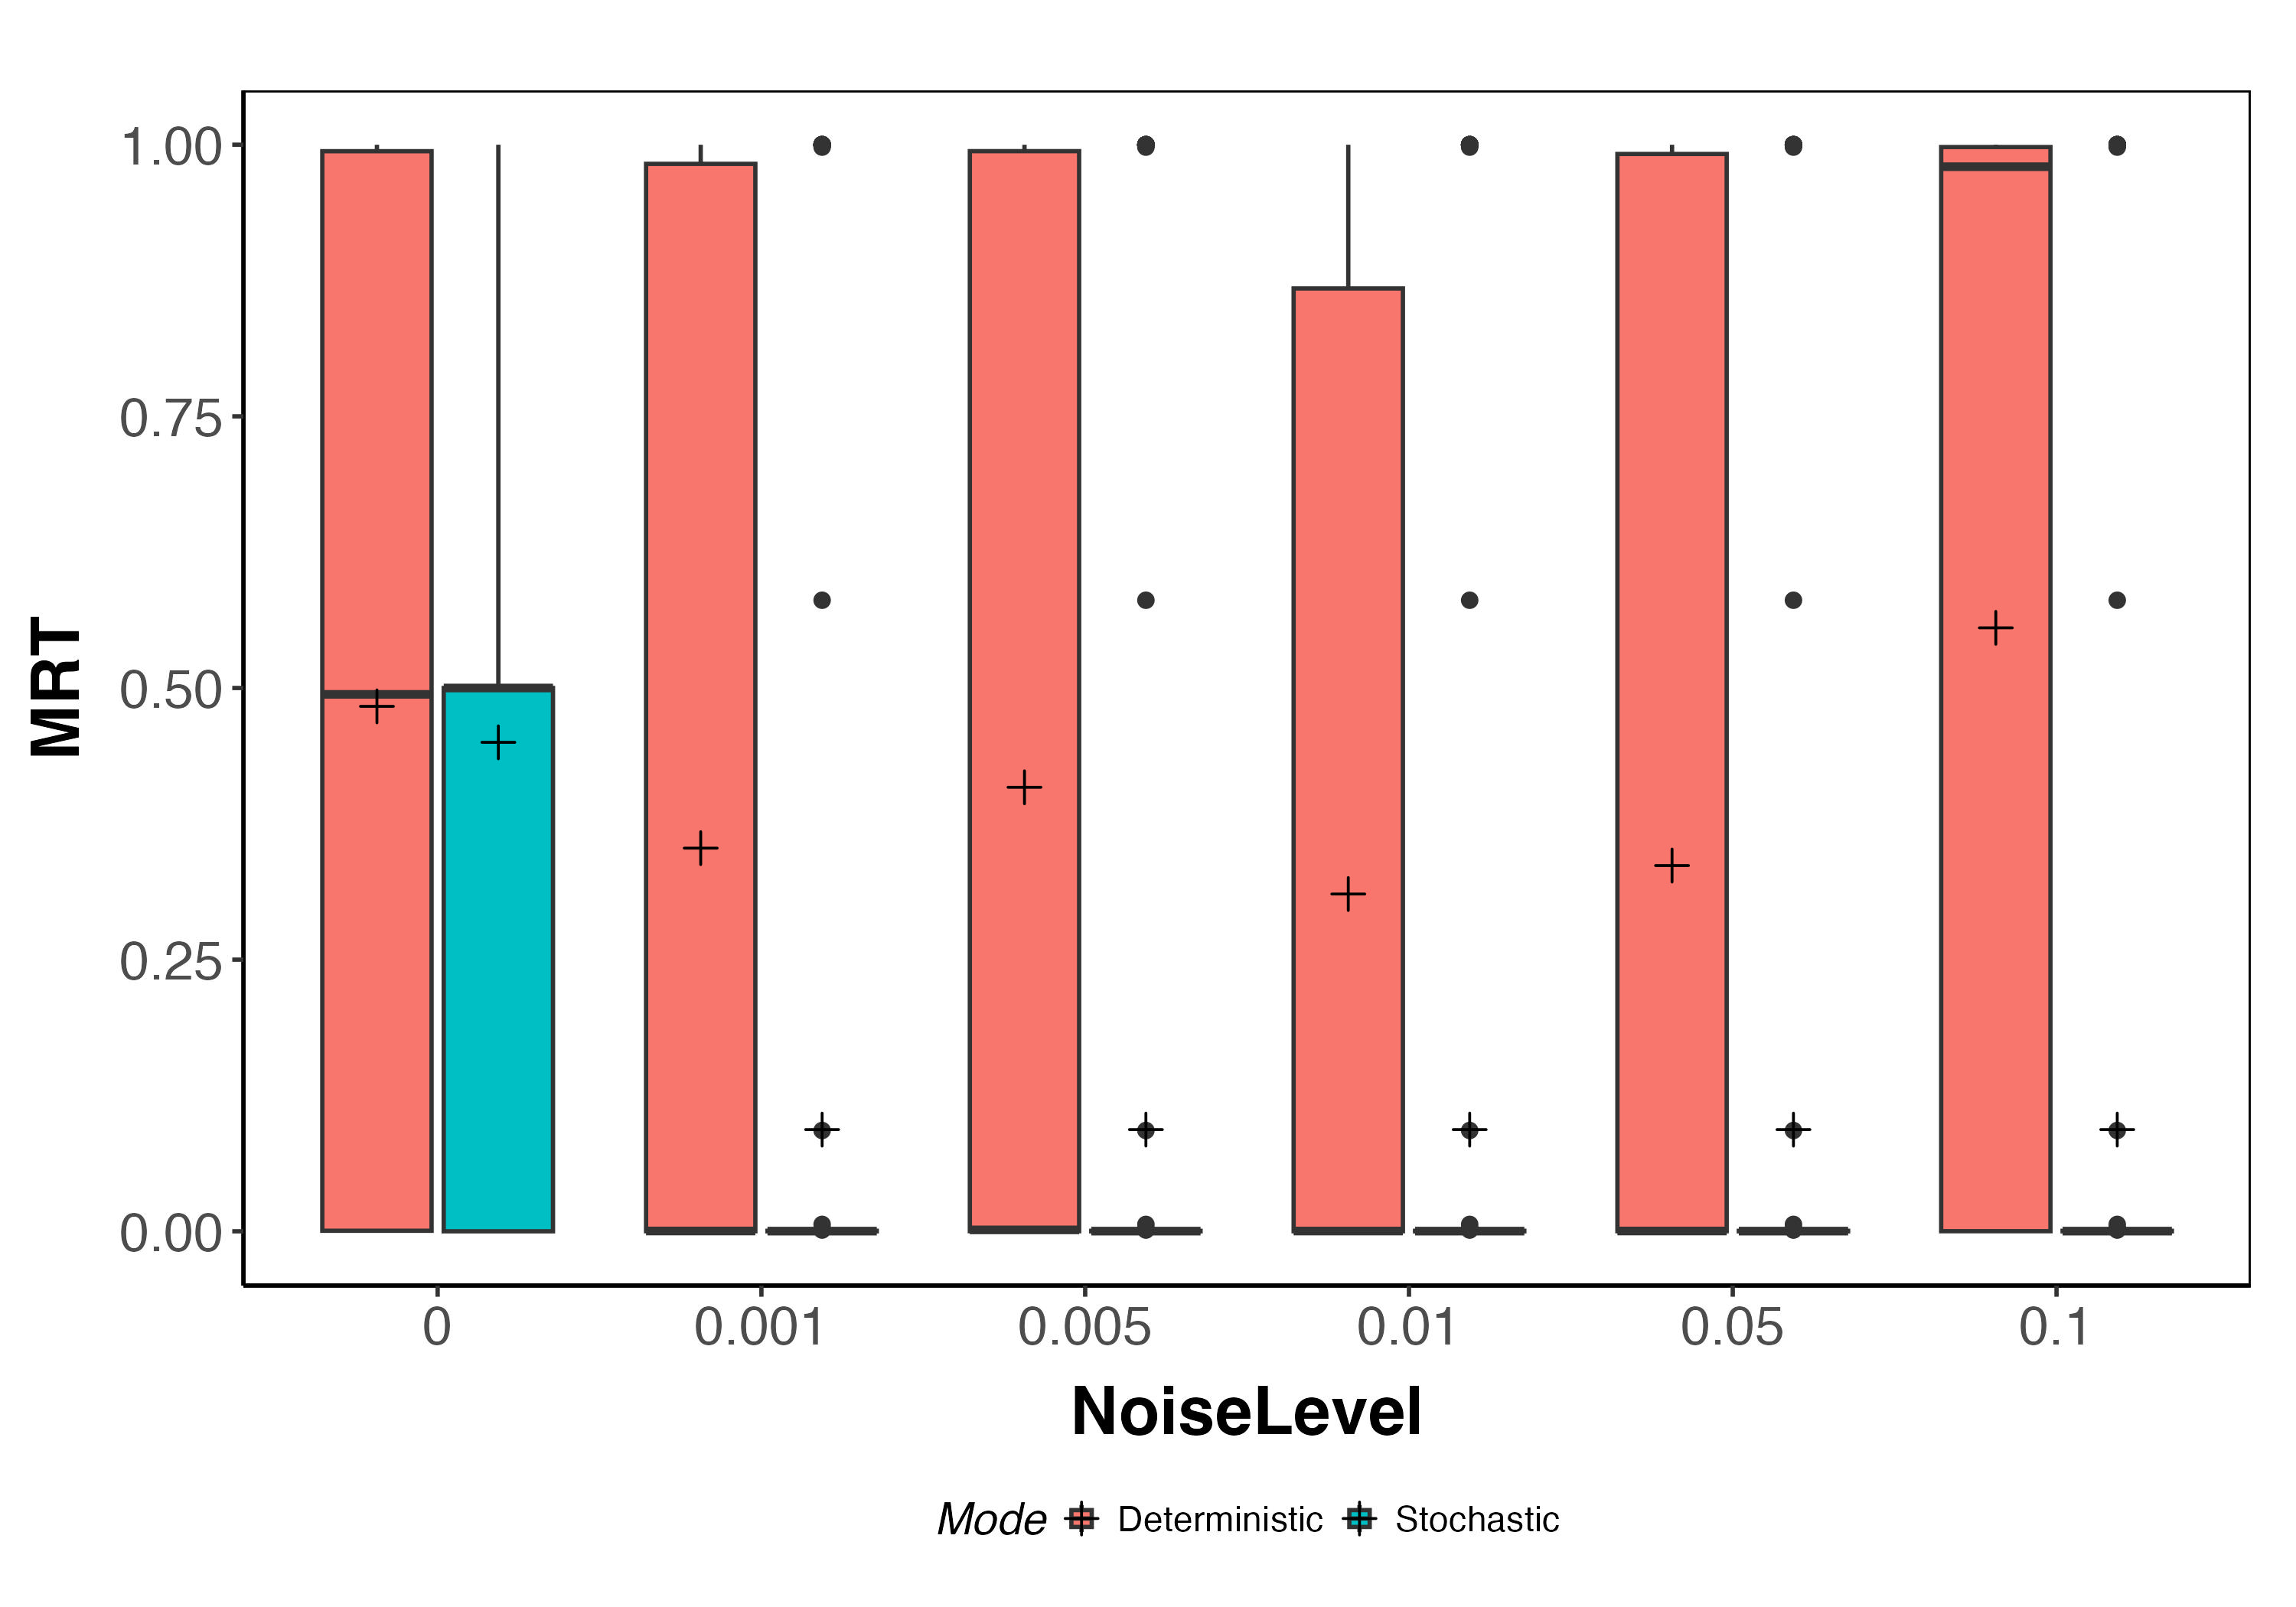
\includegraphics[width=\linewidth]{AditiveNoiseFigures/01Extreme.jpg}
%         \caption{Extreme noise}
%         \label{fig:extreme01}
%     \end{subfigure}
%     \caption{Boxplots showing the comparison of MRTs of the (0,1) state from deterministic (red) and stochastic (green) simulations of Additive, Jumping and Extreme noise. The mean of the each distribution is shown using a '+' symbol, while the median is shown by a black horizontal line segment within each box. The boundaries of the boxes show the IQR.}
%     \label{fig:01MRT}
% \end{figure}

% \section{Distribution of $\lambda$ under multiplicative noise}
\label{MultiplicativeStationary}

\subsection*{Distribution under Multiplicative Noise:
  $X \sim \mathrm{Uniform}[0,1]$, $Y = X(1 + Z)$, $Z \sim \mathcal{N}(0,\sigma^2)$}

\subsubsection*{Notation}
\begin{align*}
  x &\Rightarrow \text{current position of } \lambda \\
  y &\Rightarrow \text{next value of } \lambda \\
  z &= \frac{y}{x} - 1 \sim \mathcal{N}(0,\sigma^2) \\
  p(y \mid x) &\Rightarrow \text{conditional probability of } y \\
  p(y) &\Rightarrow \text{marginal probability of } y \\
  p_n(x) &= \frac{1}{\sqrt{2\pi}\,\sigma}
            \exp\!\left(-\frac{x^2}{2\sigma^2}\right) \\
  F_n(x_0) &= P(x \leq x_0) = \int_{-\infty}^{x_0} p_n(x)\,dx
\end{align*}

We also define the auxiliary function
\begin{equation}
  g(a) \;=\; \int_a^{\infty} \frac{p_n(t)}{1+t}\,dt,
  \label{eq:gdef}
\end{equation}
which will appear throughout. Note $g'(a) = -p_n(a)/(1+a)$.

%---------------------------------------------------------
\subsubsection*{Conditional distribution given $X = x$}

Since $Y = x(1+Z)$ and the state space is clamped to $[0,1]$:
\begin{itemize}
  \item $Y = 0$ iff $x(1+Z) \leq 0$, i.e.\ $Z \leq -1$ (for $x > 0$),
  \item $Y = 1$ iff $x(1+Z) \geq 1$, i.e.\ $Z \geq 1/x - 1$,
  \item $Y = y \in (0,1)$ otherwise, with $z = y/x - 1$.
\end{itemize}

Applying the change-of-variables $z = y/x - 1$, $dz = dy/x$:

\begin{equation}
  p(y \mid x) = \begin{cases}
    F_n(-1) & y = 0 \\[4pt]
    \dfrac{1}{x}\,p_n\!\left(\dfrac{y}{x} - 1\right) & 0 < y < 1 \\[8pt]
    1 - F_n\!\left(\dfrac{1}{x} - 1\right) & y = 1
  \end{cases}
  \label{eq:conditional_mult}
\end{equation}

%---------------------------------------------------------
\subsubsection*{Point mass at $y = 0$}

The boundary condition $Y = 0$ requires $Z \leq -1$, independently of $x$:
\begin{align*}
  p(y = 0)
    &= \int_0^1 P(Y=0 \mid X=x)\,dx
     = \int_0^1 F_n(-1)\,dx
\end{align*}
\begin{equation}
  \boxed{p(y=0) = F_n(-1)}
  \label{eq:mass0_mult}
\end{equation}

\textbf{Note:} Unlike the additive case, $p(y=0)$ depends only on $\sigma$
and not on the position $x$, because the sign change requires $Z < -1$
regardless of $x$.

%---------------------------------------------------------
\subsubsection*{Point mass at $y = 1$}

\begin{align*}
  p(y=1)
    &= \int_0^1 \left[1 - F_n\!\left(\tfrac{1}{x}-1\right)\right] dx
\end{align*}

\textbf{Substitution} $u = 1/x - 1$, so $x = 1/(1+u)$,
$dx = -du/(1+u)^2$; $x=1 \Rightarrow u=0$, $x \to 0^+ \Rightarrow u \to \infty$:

\begin{align*}
  p(y=1)
    &= \int_0^{\infty} \frac{1-F_n(u)}{(1+u)^2}\,du
\end{align*}

\textbf{IBP} with $A = 1-F_n(u)$, $dB = (1+u)^{-2}\,du$,
so $B = -(1+u)^{-1}$:

\begin{align*}
  &= \left[-\frac{1-F_n(u)}{1+u}\right]_0^{\infty}
     - \int_0^{\infty} \frac{p_n(u)}{1+u}\,du \\
  &= \left(0 - \frac{1-F_n(0)}{1}\right) - g(0) \\
  &= \frac{1}{2} - g(0)
\end{align*}

\begin{equation}
  \boxed{p(y=1) = \tfrac{1}{2} - g(0)}
  \label{eq:mass1_mult}
\end{equation}

\textbf{Note:} $p(y=0) \neq p(y=1)$ in general; the symmetry of the additive
case is broken because multiplicative noise scales with position.

%---------------------------------------------------------
\subsubsection*{Continuous density for $0 < y < 1$}

\begin{align*}
  p(y)
    &= \int_0^1 \frac{1}{x}\,p_n\!\left(\frac{y}{x}-1\right)dx
\end{align*}

\textbf{Substitution} $t = y/x - 1$, so $x = y/(1+t)$,
$dx = -y/(1+t)^2\,dt$; $x=1 \Rightarrow t=y-1$,
$x \to 0^+ \Rightarrow t \to \infty$:

\begin{align*}
  p(y)
    &= \int_{y-1}^{\infty}
       \frac{1+t}{y}\,p_n(t)\cdot\frac{y}{(1+t)^2}\,dt
     = \int_{y-1}^{\infty} \frac{p_n(t)}{1+t}\,dt
\end{align*}

\begin{equation}
  \boxed{p(y) = g(y-1), \qquad 0 < y < 1}
  \label{eq:density_mult}
\end{equation}

where $g$ is defined in Eq.~\eqref{eq:gdef}.
Note that for $y \in (0,1)$ the lower limit $y-1 \in (-1,0)$, so the
integral is always well-defined. 

%---------------------------------------------------------
\subsubsection*{CDF for $0 \leq y_0 \leq 1$}

\begin{align*}
  P(Y \leq y_0)
    &= p(y=0) + \int_0^{y_0} p(y)\,dy \\
    &= F_n(-1) + \int_0^{y_0} g(y-1)\,dy
\end{align*}

\textbf{Substitution} $s = y-1$, $ds = dy$:
\begin{align*}
  \int_0^{y_0} g(y-1)\,dy
    &= \int_{-1}^{y_0-1} g(s)\,ds
\end{align*}

\textbf{Switching order of integration} (Fubini) in
$\int_{-1}^{y_0-1} \int_s^{\infty} \frac{p_n(t)}{1+t}\,dt\,ds$:

\begin{align*}
  &= \int_{-1}^{\infty} \frac{p_n(t)}{1+t}
     \int_{-1}^{\min(t,\,y_0-1)} ds\,dt \\[4pt]
  &= \int_{y_0-1}^{\infty} \frac{p_n(t)}{1+t}\cdot y_0\,dt
   + \int_{-1}^{y_0-1} \frac{p_n(t)}{1+t}\cdot(t+1)\,dt \\[4pt]
  &= y_0\,g(y_0-1)
   + \int_{-1}^{y_0-1} p_n(t)\,dt \\[4pt]
  &= y_0\,g(y_0-1) + F_n(y_0-1) - F_n(-1)
\end{align*}

Therefore:
\begin{equation}
  \boxed{P(Y \leq y_0)
    = y_0\,g(y_0 - 1) + F_n(y_0 - 1)}
  \label{eq:CDF_mult}
\end{equation}

%---------------------------------------------------------
\subsubsection*{Sanity checks}

\textbf{At $y_0 = 0$:}
\[
  P(Y \leq 0) = 0 \cdot g(-1) + F_n(-1) = F_n(-1) = p(y=0) \;\checkmark
\]

\textbf{At $y_0 = 1$:}
\begin{align*}
  P(Y < 1) &= g(0) + F_n(0) = g(0) + \tfrac{1}{2} \\
  P(Y \leq 1) &= P(Y < 1) + p(y=1)
               = g(0) + \tfrac{1}{2} + \tfrac{1}{2} - g(0) = 1 \;\checkmark
\end{align*}

%---------------------------------------------------------
\subsubsection*{Summary}

\[
\boxed{
\begin{aligned}
  p(y=0) &= F_n(-1) \\
  p(y=1) &= \tfrac{1}{2} - g(0) \\
  p(y)\big|_{0<y<1} &= g(y-1) \\
  P(Y \leq y_0) &= y_0\,g(y_0-1) + F_n(y_0-1)
\end{aligned}
}
\]

where $g(a) = \displaystyle\int_a^{\infty} \frac{p_n(t)}{1+t}\,dt$.

\textbf{Key differences from additive noise:}
\begin{enumerate}
  \item $p(y=0) \neq p(y=1)$ in general — symmetry is broken.
  \item The continuous density $g(y-1)$ involves a non-elementary integral,
        unlike $F_n(y) - F_n(y-1)$ in the additive case.
  \item The CDF $y_0\,g(y_0-1) + F_n(y_0-1)$ must be evaluated numerically
        for general $\sigma$.
\end{enumerate}
\end{document}
